\documentclass{article}
\usepackage{booktabs}
\usepackage{graphicx}
\usepackage{amsmath}
\usepackage[a4paper, total={7in, 10.5in}]{geometry}
\usepackage[toc,page]{appendix}
\usepackage{listings} % Listing package to add appendix
\usepackage{xcolor}   % Custom colors
\definecolor{darkbrown}{rgb}{0.36, 0.2, 0.1}
\usepackage{graphicx}  % Required to include images
\usepackage{hyperref}% to put links
\usepackage{float} %to place correctly pictures
\usepackage{cite} %for better citations
\usepackage{pdfpages}
\hypersetup{
    colorlinks=true,
    linkcolor=blue,
    urlcolor=blue,
    citecolor=red,
    linktoc=all,    % Links entire section titles in the ToC
    linkcolor=black % Sets ToC links to black; other links remain as specified
}

% Defining colors for the python section
\definecolor{codegreen}{rgb}{0,0.6,0}
\definecolor{codeblue}{rgb}{0,0,0.8}
\definecolor{codepurple}{rgb}{0.58,0,0.82}
\definecolor{codebackground}{rgb}{0.95,0.95,0.92}

% Suppress page numbering on the first page
\pagenumbering{gobble}

\begin{document}

\title{Mid term Exam for Financial Econometrics with Python}
\author{PRAT Paul; GAVINI Charles; FOURNIER Justin; BLANC Mathieu}
\date{\today}

\maketitle %showcase the title in the top of the page with the informations upper

\tableofcontents %creating a table of contens
\clearpage

% Start counting pages from here
%\pagenumbering{Roman} % Preliminary content with roman figures
\pagenumbering{arabic}
\setcounter{page}{1}

%first, introduction
\section{Introduction}



This document provides a comprehensive presentation of our results, 
including all relevant tables, figures, and calculations. 
The report is structured into distinct parts, beginning with the importation of essential Python libraries. 
We then initialize variables to organize the data into different categories (e.g., daily, monthly, returns, log returns), 
allowing for clear analysis and comparison across various data types and intervals.


\section{Preliminary}
%Instructions


%At the beginning of your answer to Question 1, indicate clearly:
%- the name and the exact ticker of stock or index you are considering,
%- the length of your sample (number of days, months, years),
%- the initial and final dates of your sample, and
%- the stock market and country in which the stock you selected is traded, or to which the stock index you selected refers to.
%Using the time series you downloaded in PRELIMINARY STEP 1, compute the log-returns at daily, 
%monthly, and annual frequencies and present a table of summary statistics of these three series of returns. 
%The table should be similar to the one appearing in slide n. 91 of the set of slides titled 
%``Lecture 1: Financial Returns: Description and Stylized Facts’’.
\subsection{AMAZON}

The selected stock for this analysis is Amazon due to its significant relevance in current global markets, its impressive growth over time and its position as a major industry leader.
The ticker from yahoo finance is "\textbf{\textit{AMZN}} " on the Nasdaq stock exchange \href{https://finance.yahoo.com/quote/AMZN/.}{AMAZON on Yahoo Finance}
First, importing the Amazon stock with yfinance, then display the pandas table.
We will import 25 years, 8 months and 25 days of data (from 1999-01-21 to 2024-10-16).

\subsection{Data Table}
The data printed here is the preview of the Amazon stock extraction from yahoo finance:
% LaTeX table from 'table.tex'
\begin{table}[h!]
    \centering
    \begin{tabular}{lrrrrrr}
\toprule
{} &      Open &      High &       Low &     Close &  Adj Close &     Volume \\
Date       &           &           &           &           &            &            \\
\midrule
1999-09-16 &  0.051563 &  0.052083 &  0.050260 &  0.050911 &   0.046693 &  158112000 \\
1999-09-17 &  0.050586 &  0.051042 &  0.048958 &  0.050781 &   0.046574 &  171648000 \\
1999-09-20 &  0.049870 &  0.050521 &  0.048958 &  0.048958 &   0.044902 &  229104000 \\
1999-09-21 &  0.047917 &  0.048177 &  0.043620 &  0.044271 &   0.040603 &  737328000 \\
1999-09-22 &  0.044271 &  0.045573 &  0.041667 &  0.045313 &   0.041559 &  375984000 \\
\bottomrule
\end{tabular}
  
    \caption{Preview of Amazon Stock Data (5 first datas) from "AMZN" in Yahoo Finance}
    \label{tab:amazon_stock_preview}
\end{table}



\subsection{Checking the 25 Years range condition}


We need to verify that the data displays accurately over the 25 years range. 
Fortunately, the extracted  Amazon data has been available since January 1999. 
To ensure the data’s continuity and completeness, we will implement a Python script that identifies and counts any gaps within the dataset. 
By visualizing the dates of these gaps, we can easily detect any significant interruptions that could potentially impact our data analysis

\begin{figure}[H]
    \centering
    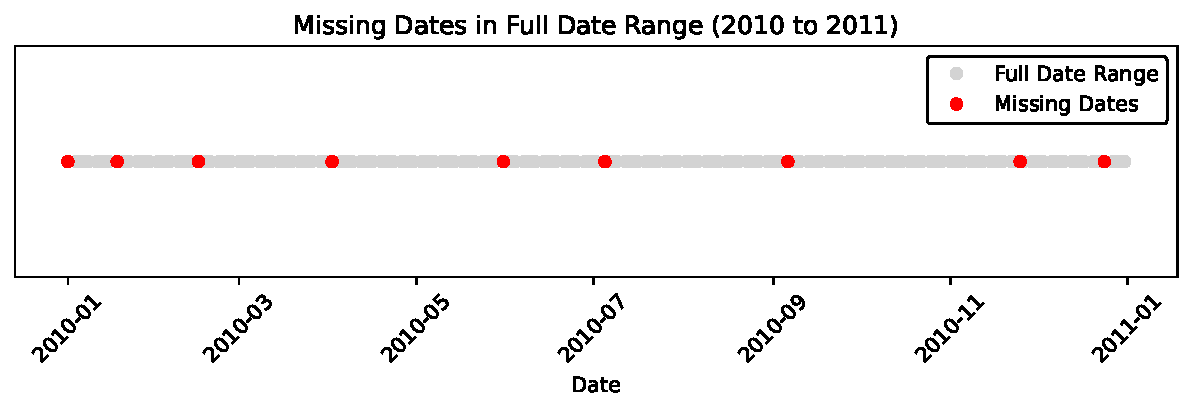
\includegraphics[width=0.8\textwidth]{Img/MissingDates(2010_to_2011).pdf}
    \caption{Missing Dates in a partial date range (\textbf{01-01-2010} to \textbf{01-01-2011})}
    \label{fig:missing_dates}
\end{figure}

\noindent We identified a total of 238 isolated days of data gaps per year across the 25-years range (6476 values). 
Therefore, the data remains reliable for our stylized facts analysis. 
The missing data points in our dataset are randomly distributed and account for 3.7\% of the total data. 
According to scientific studies on data reliability for volatility testing, a dataset with up to 10% missing data is considered reliable for statistical testing.
\cite{pumi2023longrange} 

\section{First Results}

\subsection{Prices Evolutions}

With the accuracy and the reliability of our dataset confirmed, we begin by plotting the evolution of prices over 4 different periods : Daily, Weekly, Monthly and Yearly prices.

\begin{figure}[H]
    \centering
    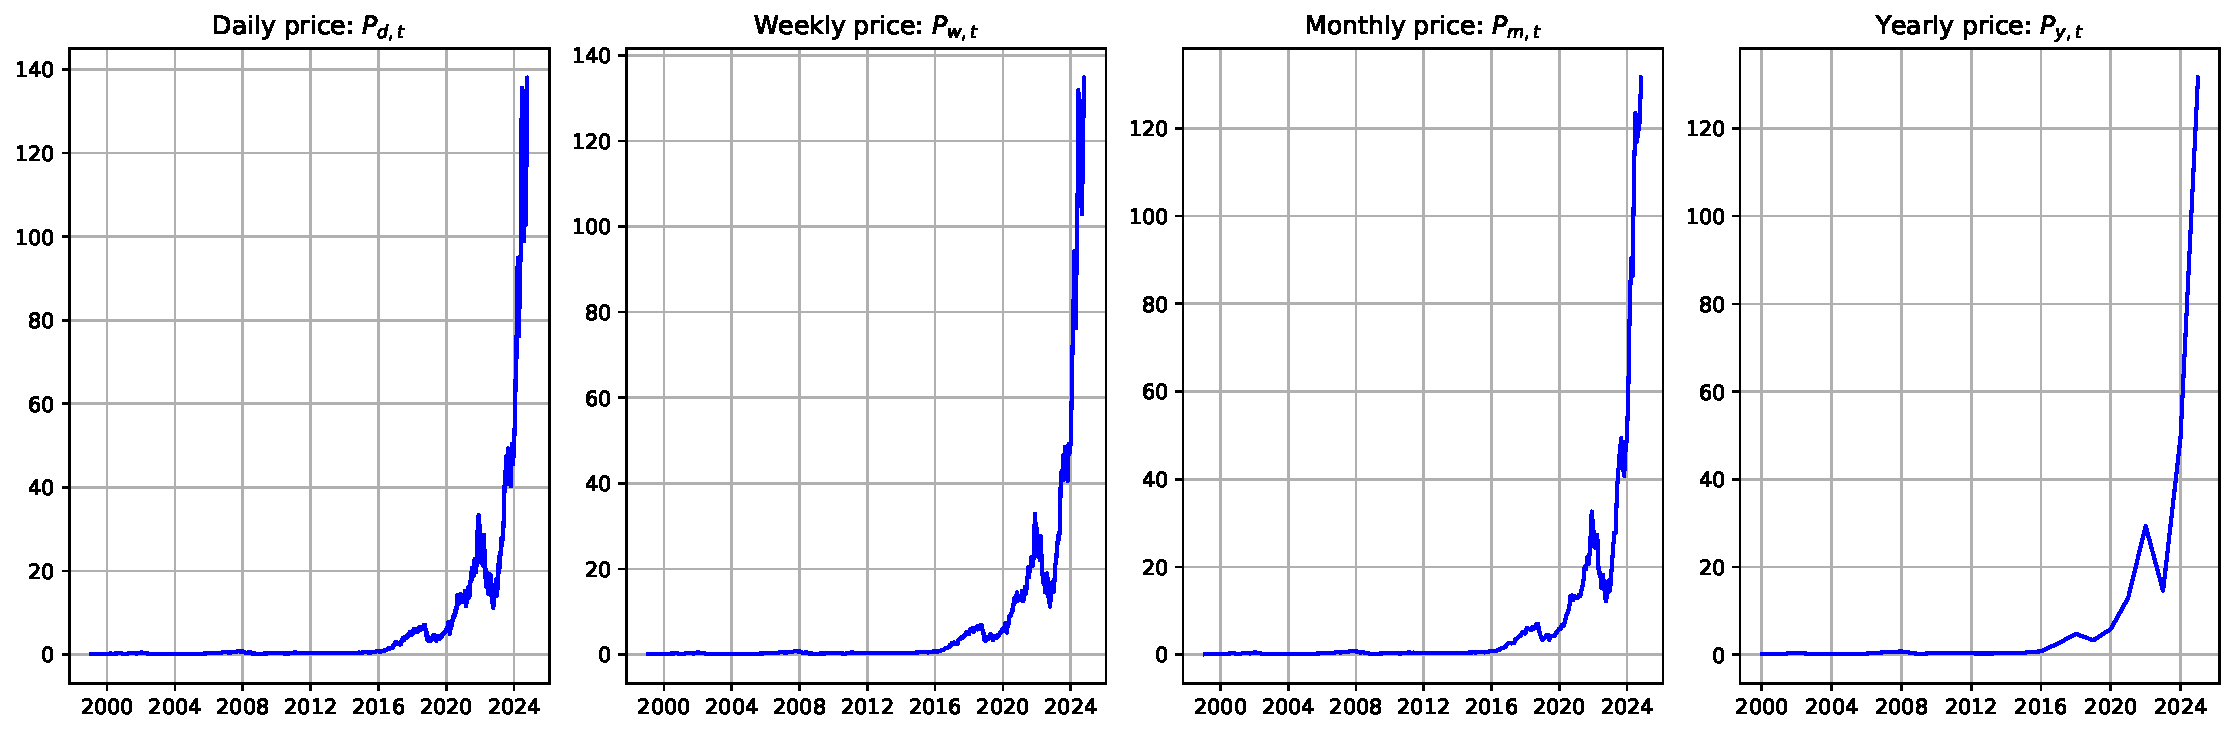
\includegraphics[width=\textwidth]{Img/prices_time.pdf}
    \caption{Prices over time $P_t$  by frequency daily, weekly, monthly and annual the AMZN stock.
    Sample: \textbf{01-21-1999} to \textbf{10-16-2024}.}
    \label{fig:prices_time}
\end{figure}

\subsection{Calculating Returns}
Using the processed data, we can now output graphs for several key metrics: 
daily prices, daily log prices, daily simple returns, and daily log returns. 
Plotting these metrics will allow us to observe daily price movements, 
the transformation of prices into $log$ form for trend analysis, 
as well as daily returns and their logarithmic equivalents.
\begin{figure}[H]
    \centering
    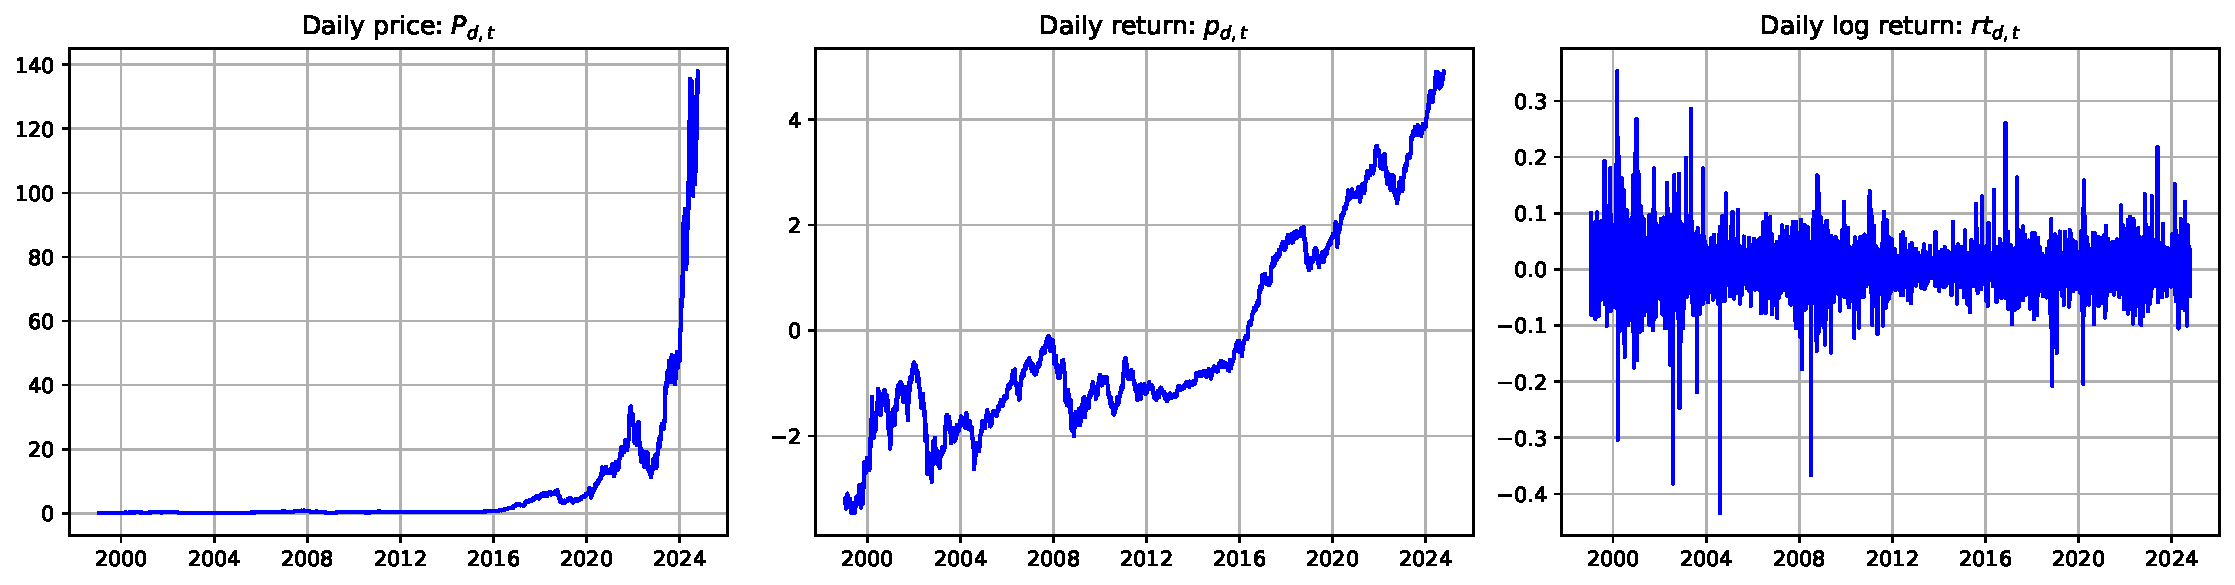
\includegraphics[width=\textwidth]{Img/log_returns.pdf}
    \caption{Prices $P_t$, returns $R_t$ and log returns $r_t$ of the AMZN stock.
    Sample: \textbf{01-21-1999} to \textbf{10-16-2024}.}
    \label{fig:log_returns}
\end{figure}

%\subsection{Squared Returns}
%
%To complete the analysis of daily price data, we also plot the daily squared returns and daily squared log returns, 
%(providing us a key insight on the volatile behavior on the potential stock risk of our data set.)
%\begin{figure}[H]
%    \centering
%    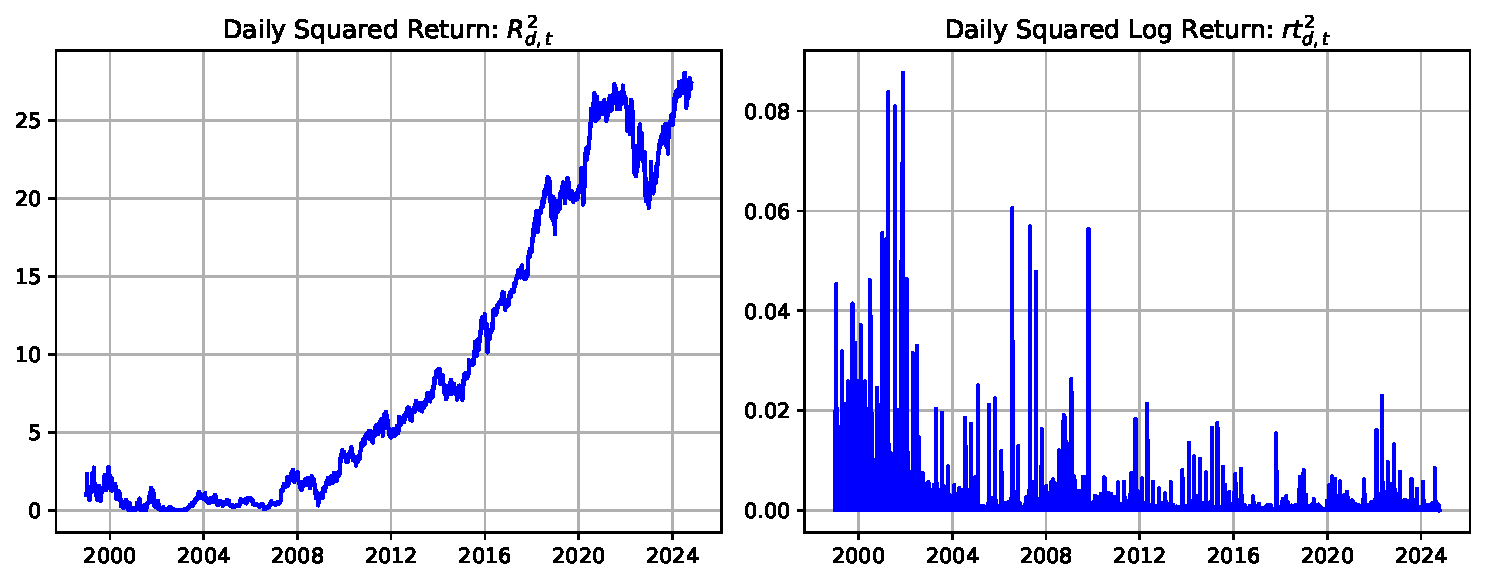
\includegraphics[width=0.8\textwidth]{Img/squared_log_returns.pdf}
%    \caption{Squared daily returns $R_t^2$ and daily squared log returns $r_t^2$ of the AMZN stock.
%    Sample: \textbf{01-21-1999} to \textbf{10-16-2024}.}
%    \label{fig:squared_logreturns}
%\end{figure}

\clearpage
% Start main content with Arabic numbering from 1
%\pagenumbering{arabic}
%\setcounter{page}{1}

\section{Amazon and the 8 Stylized Facts}

\subsubsection{Summary statistics}


\begin{table}[H]
    \centering
    \begin{tabular}{lrrrr}
\toprule
{} &        daily &      weekly &    monthly &     annual \\
\midrule
Mean                    &      0.06351 &     0.31014 &    1.32164 &   22.85692 \\
St.Deviation            &      3.24131 &     6.76830 &   13.06275 &   45.28052 \\
Diameter.C.I.Mean       &      0.07896 &     0.36213 &    1.45887 &   18.11598 \\
Skewness                &      0.41992 &     0.05008 &   -0.45895 &   -0.15137 \\
Kurtosis                &     11.15158 &     7.60655 &    2.59462 &   -0.64793 \\
Excess.Kurtosis         &      8.15158 &     4.60655 &   -0.40538 &   -3.64793 \\
Min                     &    -28.45678 &   -38.51804 &  -53.02674 &  -68.54809 \\
Quant5                  &     -4.61051 &    -9.74288 &  -20.16713 &  -55.72274 \\
Quant25                 &     -1.25994 &    -2.64062 &   -4.98163 &   -7.23999 \\
Median                  &      0.04108 &     0.30519 &    2.09626 &   23.07665 \\
Quant75                 &      1.39659 &     3.40897 &    8.45973 &   55.96192 \\
Quant95                 &      4.47118 &    10.67416 &   20.90661 &   94.77653 \\
Max                     &     29.61811 &    56.11507 &   48.35221 &  102.44636 \\
Jarque.Bera.stat        &  33735.75720 &  3235.87866 &   97.20696 &    0.51147 \\
Jarque.Bera.pvalue.X100 &      0.00000 &     0.00000 &    0.00000 &   77.43487 \\
Lillie.test.stat        &      0.10194 &     0.09591 &    0.08194 &    0.06494 \\
Lillie.test.pvalue.X100 &      0.10000 &     0.10000 &    0.10000 &   99.00000 \\
N.obs                   &   6474.00000 &  1342.00000 &  308.00000 &   24.00000 \\
\bottomrule
\end{tabular}
  
    \caption{Summary statistics for the AMZN stock.
    Sample: \textbf{01-21-1999} to \textbf{10-16-2024}.}
    \label{tab:Stylized_facts_preview}
\end{table}


% refering to the table with : Table~\ref{tab:Stylized_facts_preview}

\subsection{Prices are non-stationary}

The first feature that will highlight non-stationarity of
the prices is the comparison of \( p_t \) vs \( p_{t-1} \).

\begin{figure}[H]
    \centering
    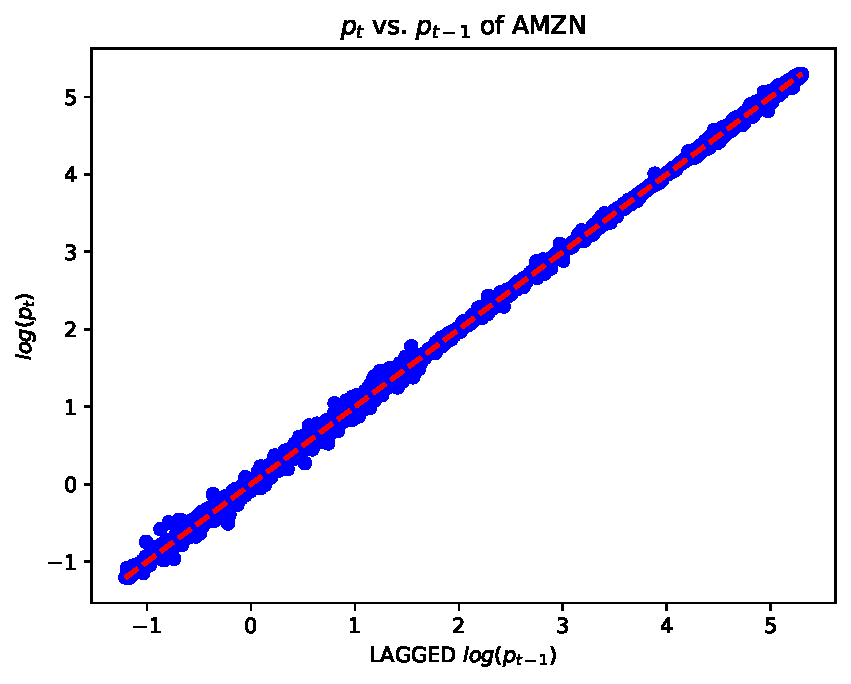
\includegraphics[width=0.5\textwidth]{Img/Laggedlog(p_t-1).pdf}
    \caption{Comparison of \( \log(p_t) \) vs \( \log(p_{t-1}) \) of the AMZN stock.
    Sample: \textbf{01-21-1999} to \textbf{10-16-2024}.}
    \label{fig:LogptVSLogpt-1}
\end{figure}

\noindent The graph in Figure \ref{fig:LogptVSLogpt-1} demonstrates this strong linear 
relationship, indicating that Amazon's prices at time \( t \) are highly dependent on those at \( t-1 \) and lack mean reversion,
 supporting the idea of non-stationarity.

\noindent Additionally, the empirical autocorrelation function (ACF) of Amazon's daily prices shows a slow decay, further suggesting non-stationarity, as shown in the next figure.

\begin{figure}[H]
    \centering
    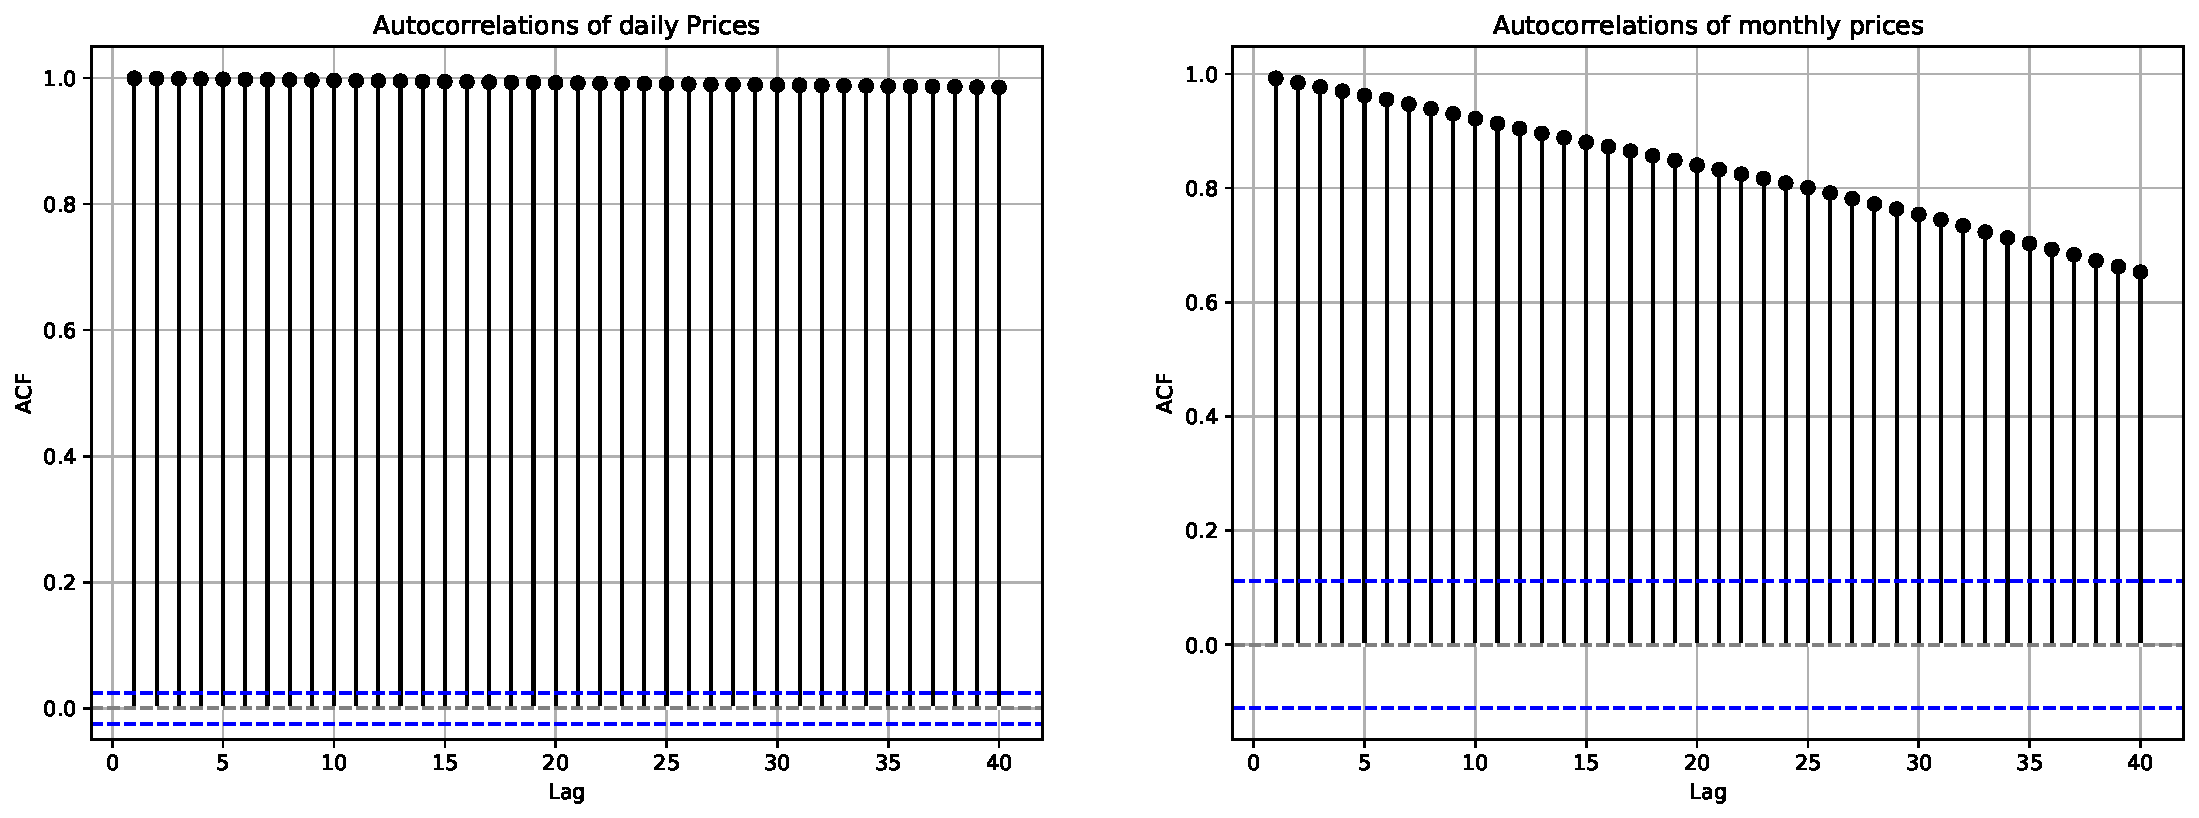
\includegraphics[width=0.8\textwidth]{Img/Autocorrel_daily_monthly.pdf}
    \caption{Autocorrelations of daily and monthly prices of the AMZN stock.
    Sample: \textbf{01-21-1999} to \textbf{10-16-2024}.}

    \label{fig:Autocorrelations_daily_monthly}
\end{figure}

\noindent For the amzon daily and monthly prices time series, we expect to see large values of $\hat{\rho}_k$, i.e., near to 1, slowly decaying as $k$ increases this is the \textbf{long memory property}.
Also, the \textbf{slowly decaying ACF} is often a symptom of non stationarity.
\subsection{Returns are stationary}

\begin{figure}[H]
    \centering
    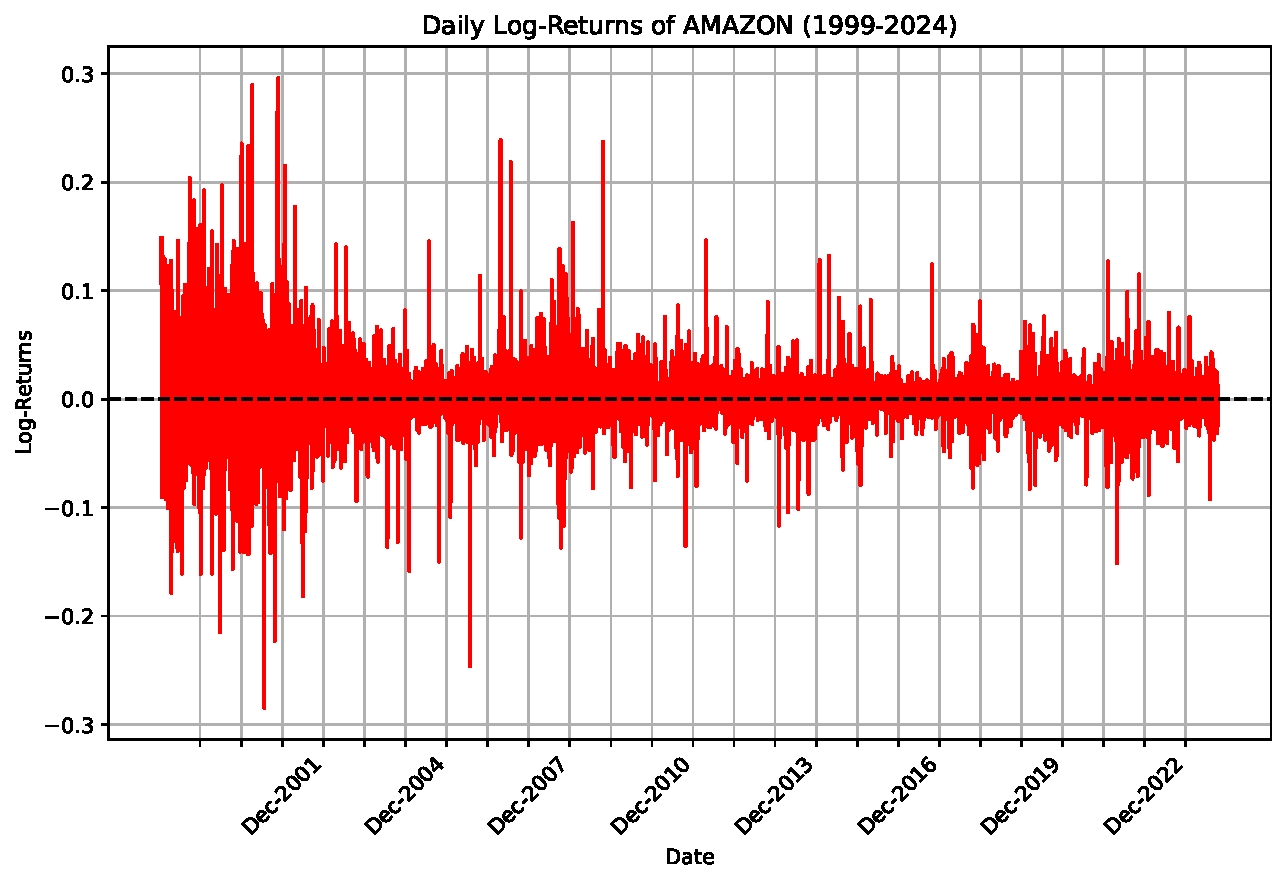
\includegraphics[width=0.5\textwidth]{Img/Daily_Log_Returns.pdf}
    \caption{Daily Log-returns $r_t := p_t - p_{t-1}$ of the AMZN stock.
    Sample: \textbf{01-21-1999} to \textbf{10-16-2024}.}
    \label{fig:Daily_log_returns}
\end{figure}

\noindent $Log$-returns are a common way to measure the percentage change in stock prices, 
and they help assess the stability or stationarity of the returns over time. In a stationary series, we would expect the properties, 
such as mean and variance, to remain constant over time. 
However, here we observe significant differences in volatility across the timeline. \\

\noindent In the early years (around 1999-2005), there is noticeably higher volatility in Amazon's log-returns, 
with frequent large spikes both upwards and downwards. This period corresponds to the tech boom and subsequent dot-com bubble burst, 
during which many tech stocks, including Amazon, experienced extreme price fluctuations. 
Additionally, as a relatively new and fast-growing company, Amazon’s stock likely faced higher uncertainty and speculative trading, 
contributing to greater volatility.

\subsection{Asymmetry}

\begin{figure}[H]
    \centering
    \begin{minipage}{0.45\textwidth}
        \begin{table}[H]
            \centering
            \begin{tabular}{lrrrr}
\toprule
{} &     daily &   weekly &  monthly &   annual \\
\midrule
Skewness &   0.39404 &  0.04813 & -0.46401 & -0.99033 \\
Kurtosis &  11.04424 &  7.51963 &  2.60379 &  1.46124 \\
\bottomrule
\end{tabular}
  
            \caption{\textbf{Skewness and kurtosis of daily, weekly, monthly and annual} $log$ returns of the AMZN stock. 
            Sample: \textbf{01-21-1999} to \textbf{10-16-2024}.}
            \label{tab:skewness_kurtosis}
        \end{table}
    \end{minipage}
    \hspace{0.05\textwidth}
    \begin{minipage}{0.45\textwidth}
        \centering
        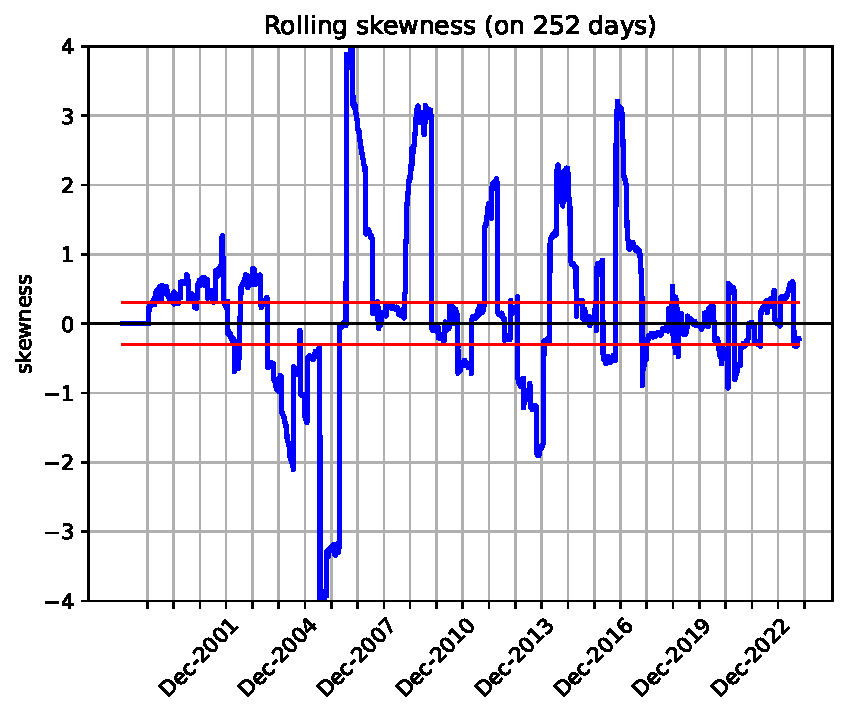
\includegraphics[width=0.8\textwidth]{Img/Fact3_2_rollskew.pdf}
        \caption{\textbf{Rolling skewness} of AMZN stock. 
        Sample: \textbf{01-21-1999} to \textbf{10-16-2024}. The \textcolor{red}{red bands} corresponds to the limit of acceptance, the blue line correspond to the rolling skewness with T=252}
        \label{fig:Rolling_skewness}
    \end{minipage}
\end{figure}

\noindent For this case, Table~\ref{tab:skewness_kurtosis} hilights that for daily returns the AMZN stock skewness is positive.
This does not confirms stylized fact 3, this case is not really common but it means that the mean return is higher than the median of the sample \cite{albuquerque2012skewness}. 
Then, Amazon investors tend to have steeper high turns than downturns and that investors of the AMZN stock react more positively to good news than they can react badly for negative news.
If we take a look at the Rolling Skewness on simple returns Figure~\ref{fig:Rolling_skewness}, we clearly see that the skewness (for a 252 days interval) varies a lot depending the position of intervals and has already been very negative (Dec 2004) but is generally positive.
\subsection{Heavy tails}
\noindent As showcased in the Table~\ref{tab:skewness_kurtosis}, there is a large excess kurtosis

\begin{figure}[H]
    \centering
    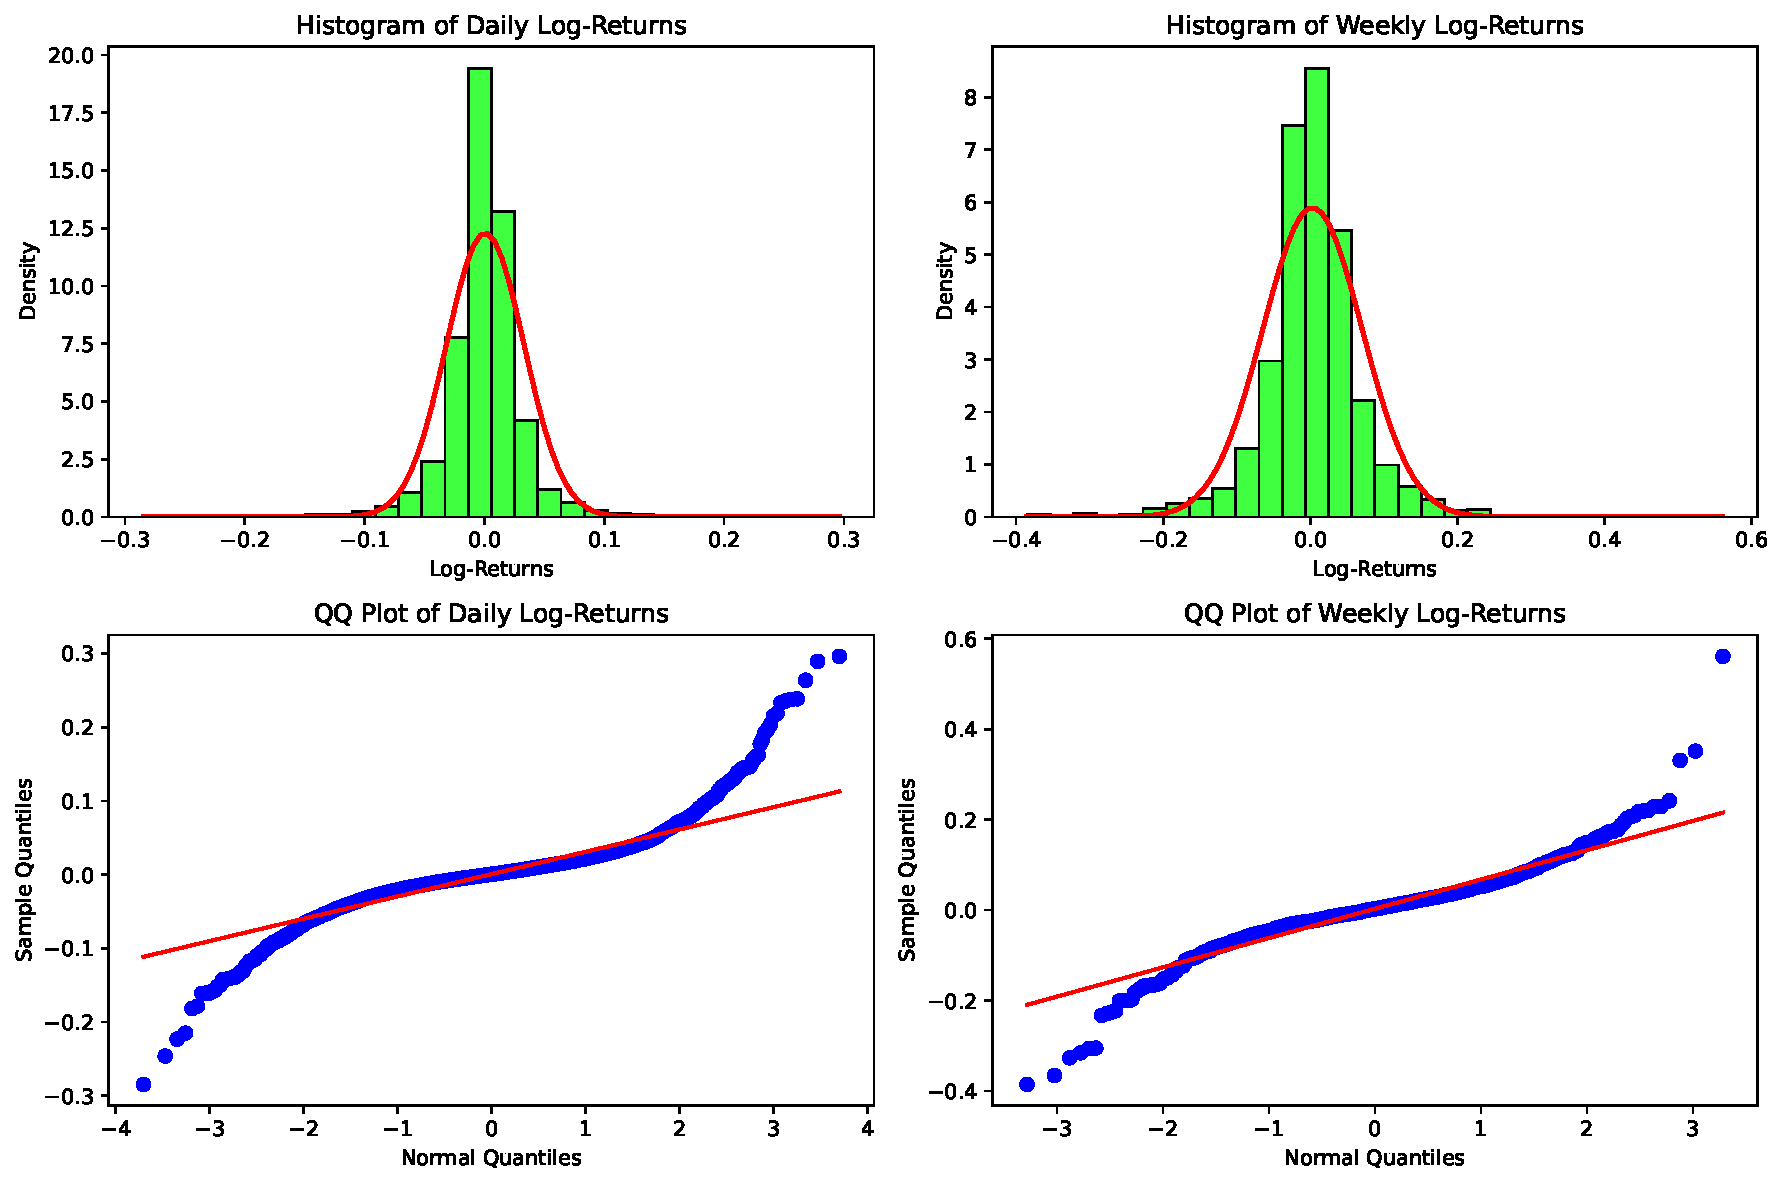
\includegraphics[width=0.6\textwidth]{Img/QQplot_daily_weekly_AMZN.pdf}
    \caption{Log returns $r_t := p_t - p_{t-1}$: \textbf{histograms of daily, monthly} “adjusted closing” of AMAZON. 
    Sample: \textbf{01-21-1999} to \textbf{10-16-2024}. QQ plot against quantiles of normal distribution with same mean and variance as the empirical distribution of returns.}
    \label{fig:Hstogram_QQ_plot}
\end{figure}

\noindent Here, the QQ-Plots explicit clearly how our sample distinguishes from the normal distribution. 
The QQ-plot provide graphical evidence that the tails of the daily returns distributions are heavier than the tails of the normal distribution as: The points on the left of the graph which represent the lower quantiles (i.e. the points in the left tail of the empirical distribution) are below the blue line. The lower quantiles of the empirical distribution are much smaller than what you should expect from a Normal random variable with the same empirical mean and standard deviation of the sample the left tail of the empirical distribution is heavier than one of a Normal Distribution. similar conclusions for the right tail.
\begin{figure}[H]
    \centering
    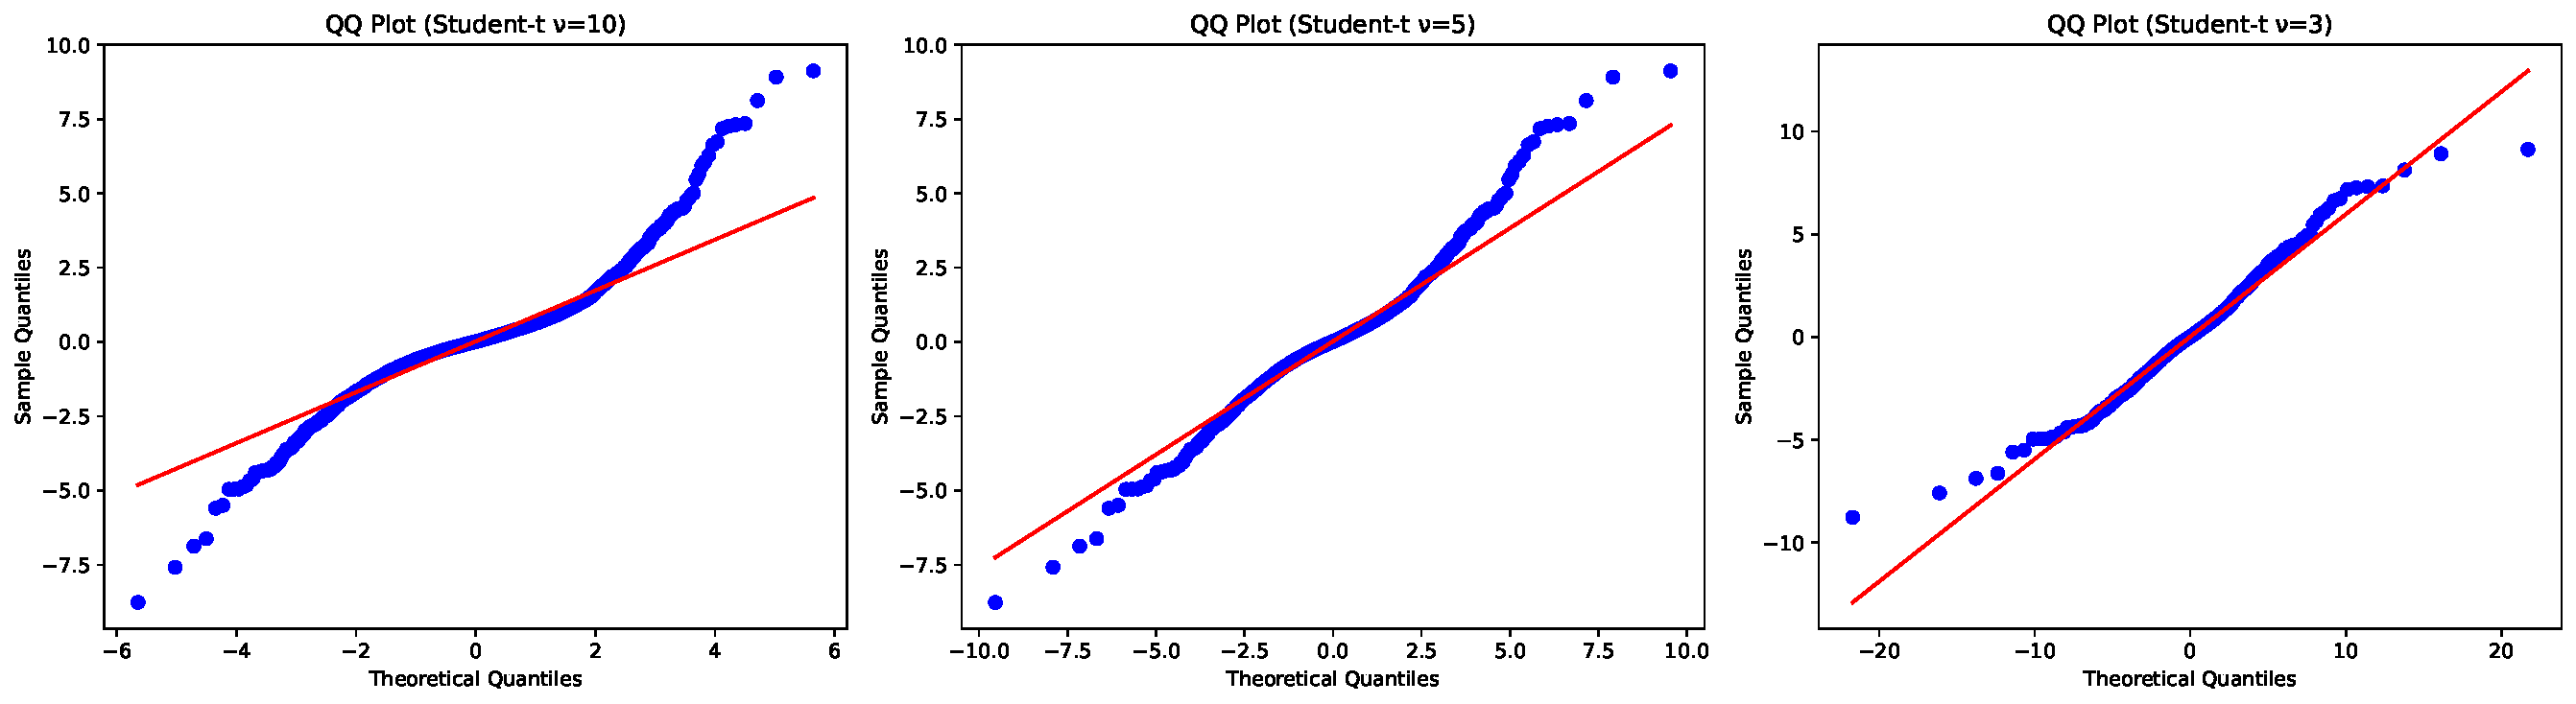
\includegraphics[width=1\textwidth]{Img/qqplt_tstudents_AMZNdaily.pdf}
    \caption{Log returns $r_t := p_t - p_{t-1}$: \textbf{daily} “adjusted closing” of AMZN stock. 
    Sample: \textbf{01-21-1999} to \textbf{10-16-2024}. \textbf{QQ plot of Sample standardized quantiles} (0 mean and unit variance) \textbf{of daily log-returns against quantiles of standardized} (0 mean and unit variance) \textbf{Student-t distributions} with $\nu = 10$, 5, and 3 degrees of freedom.}
    \label{fig:Hstogram_QQ_plot_T_student}
\end{figure}
\subsection{Gaussianity}
\subsubsection{High frequency non-Gaussianity}

The aggregate gaussianity, states that lower frequency returns (monthly) tend to be Gaussian (symmetric about the mean) even if higher frequency returns (daily) are not. 
To test this stylized fact we perform a Jarge-Bera test. The result is in Table~\ref{tab:Stylized_facts_preview}. \\

\noindent The 3\textsuperscript{rd} central moment is defined as
$\mu_3 := E((X - m_1)^3).$ The skewness of \( r_t \) is defined as:
\[
\text{Skew}(r_t) := E \left[ \left( \frac{X - m_1}{\sigma} \right)^3 \right] = \frac{\mu_3}{\sigma^3} = \frac{\mu_3}{\mu_2^{3/2}}.
\]

\noindent As the result in Table~\ref{tab:Stylized_facts_preview} 
the skewness is positive for daily and monthly data, \( \text{Skew}(r_t) >0 \), large realizations of \( X \) are more often larger
than the mean \( \mu \). 
Skewness is thus used as a measure of asymmetry of the distribution \( f_X(x) \). Therefore:
 
\( \text{Skew}(r_t) > 0 \), so the distribution is said to be \textbf{right skewed}. 
%For symmetric distributions (e.g., Gaussian, t-Student, uniform), 
%we have \( \text{Skew} = 0 \). In these cases, all odd moments are zero:
%\( \mu_r = E[(X - \mu)^3] = 0 \) for \( r = 3, 5, \dots \)

\( \text{Skew}(r_t) > 0 \), then \( \mu > \text{median} \).

\subsubsection{Aggregational Gaussianity}
\begin{figure}[H]
    \centering
    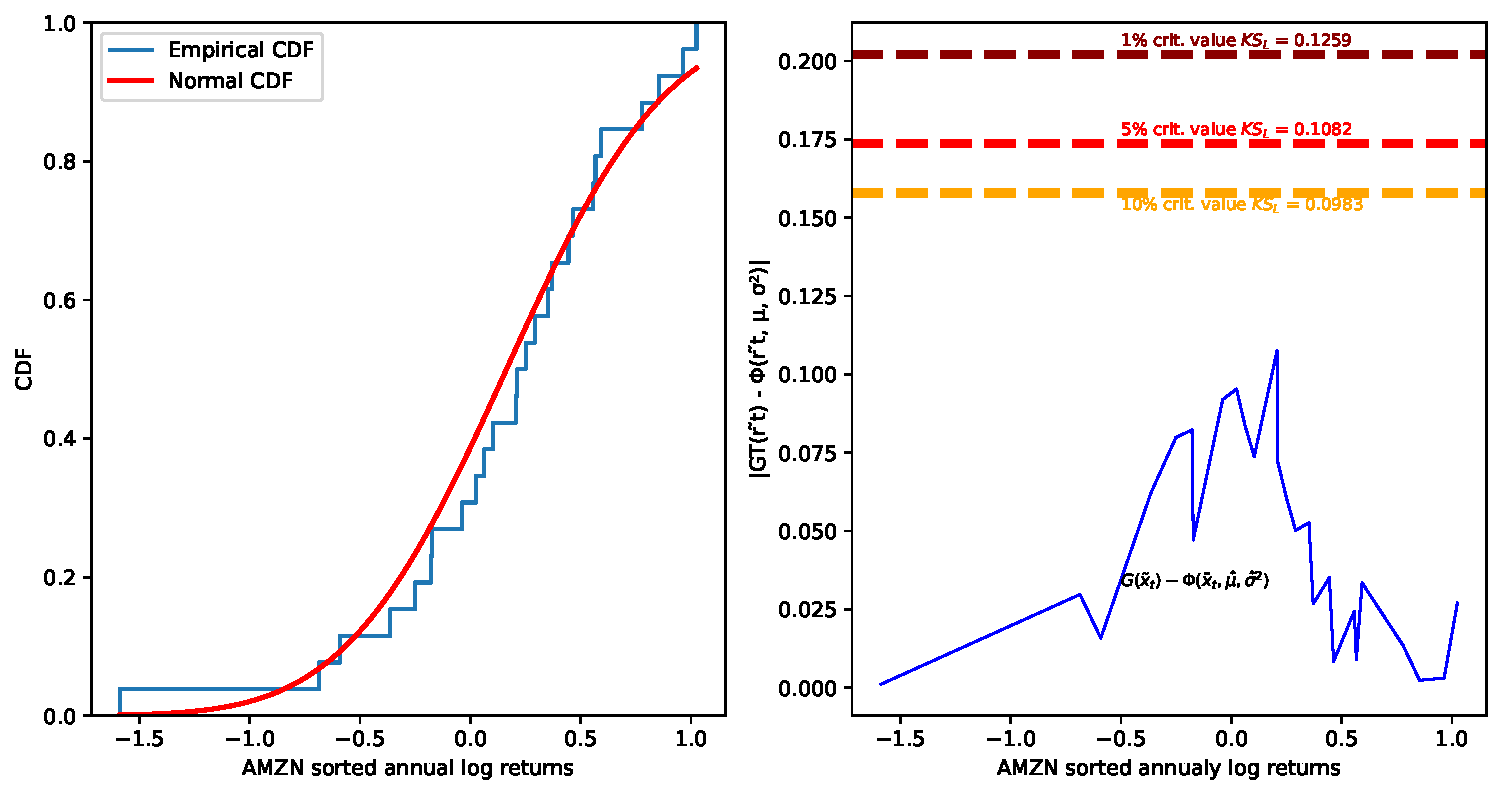
\includegraphics[width=0.8\textwidth]{Img/lillie_test_AMZNannualy.pdf}
    \caption{Log returns $r_t := p_t - p_{t-1}$: \textbf{annual} “adjusted closing” of AMZN. 
    Sample: \textbf{01-21-1999} to \textbf{10-16-2024}. \textbf{Left panel}: empirical and Normal cdf's for the standardized annual returns of AMZN. \textbf{Right panel}: values of $\left| G_T(\tilde{r}_t) - \Phi(\tilde{r}_t, \hat{\mu}, \hat{\sigma}^2) \right|$ (\textcolor{blue}{blue line}) and critical values for the Lilliefors test for the three significance levels \textcolor{orange}{10\%}, \textcolor{red}{5\%} and \textcolor{darkbrown}{1\%}.}
    \label{fig:Lillie_test_weekly}
\end{figure}

\noindent The blue line is under the critical values lines, 
So the test is respected and so for the Gaussianity.
\subsection{Returns are not autocorrelated}

Stylised fact 6 posits that returns are not autocorrelated. 
Autocorrelation in a weakly stationary process measures the correlation between values of the process at different time points. 
To assess the significance of autocorrelations, we apply the \textbf{Box-Pierce (BP)} test or the \textbf{Ljung-Box (LB)} test, 
where the null hypothesis indicates that all autocorrelations are equal to 0, compared with the alternative analysis where it differs from 0.

\begin{table}[H]

    \centering
    \begin{tabular}{lrrrrrrrrr}
\toprule
{} &  lag &    acf &  acf diam. &  acf test &  B-P stat &  B-P pval &  L-B stat &  L-B pval &    crit \\
\midrule
0  &    1 &  0.053 &      0.112 &     0.930 &     0.865 &     0.352 &     0.874 &     0.350 &   3.841 \\
4  &    5 &  0.021 &      0.112 &     0.376 &     7.654 &     0.176 &     7.796 &     0.168 &  11.070 \\
14 &   15 & -0.049 &      0.112 &    -0.865 &    22.975 &     0.085 &    23.673 &     0.071 &  24.996 \\
\bottomrule
\end{tabular}
  
    \caption{Ljung-Box and Box-Pierce daily}
    \label{tab:LB_BP}
\end{table}
In Table~\ref{tab:LB_BP}, we observe that for each lag (1, 5, 15 and 25), the p-values for both the \textbf{Ljung-Box (L-B pval)} and \textbf{Box-Pierce} ($B-P pval$) tests exceed the \textbf{$0.048$ threshold}. This indicates that there is insufficient statistical evidence to reject the null hypothesis at each lag. Consequently, this suggests that the returns are not significantly autocorrelated across these time lags.
\subsection{Volatility clustering and long range dependence of squared returns}

Volatility clustering is a phenomenon where periods of high market volatility are often followed by high volatility, and vice versa. To capture and analyze this phenomenon, financial models such as ARCH (Autoregressive Conditional Heteroskedasticity) and GARCH are commonly used. We can easily perceive it on the graph below, (from december 2001 to december 2004) phase of low volatility.

\begin{figure}[H]
    \centering
    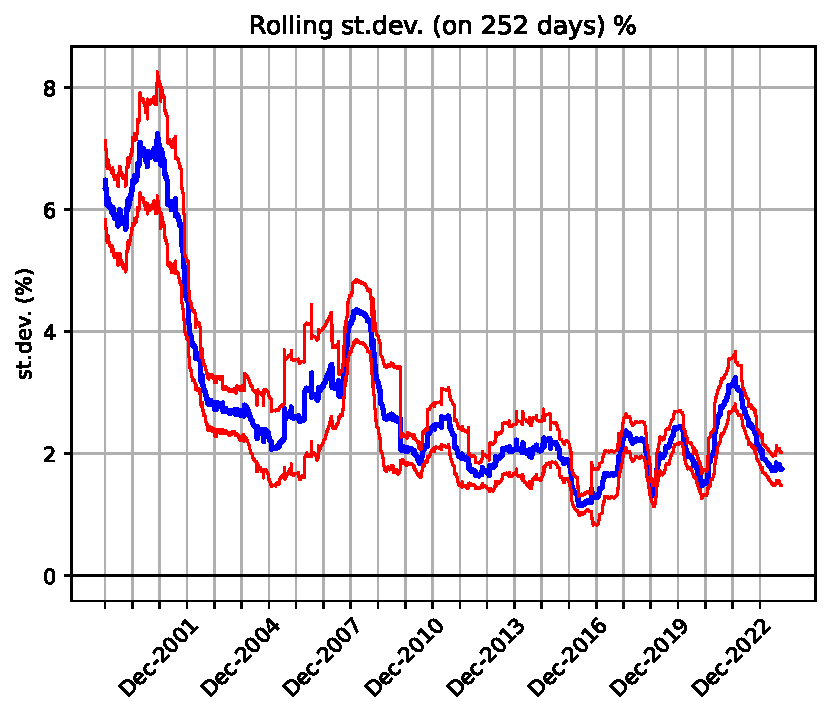
\includegraphics[width=0.5\textwidth]{Img/Fact7_AMZN_rolling_stdev.pdf}
    \caption{Rolling standard deviation from the “adjusted closing” of AMZN. Sample: \textbf{01-21-1999} to \textbf{10-16-2024}.}
    \label{fig:Rolling_std_dev_1}
\end{figure}

\noindent This persistence in the autocorrelation of squared returns reflects volatility clustering. 
High volatility often persists over time before settling into a lower volatility regime; 
this is how time dependance is reflected.



\begin{figure}[H]
    \centering
    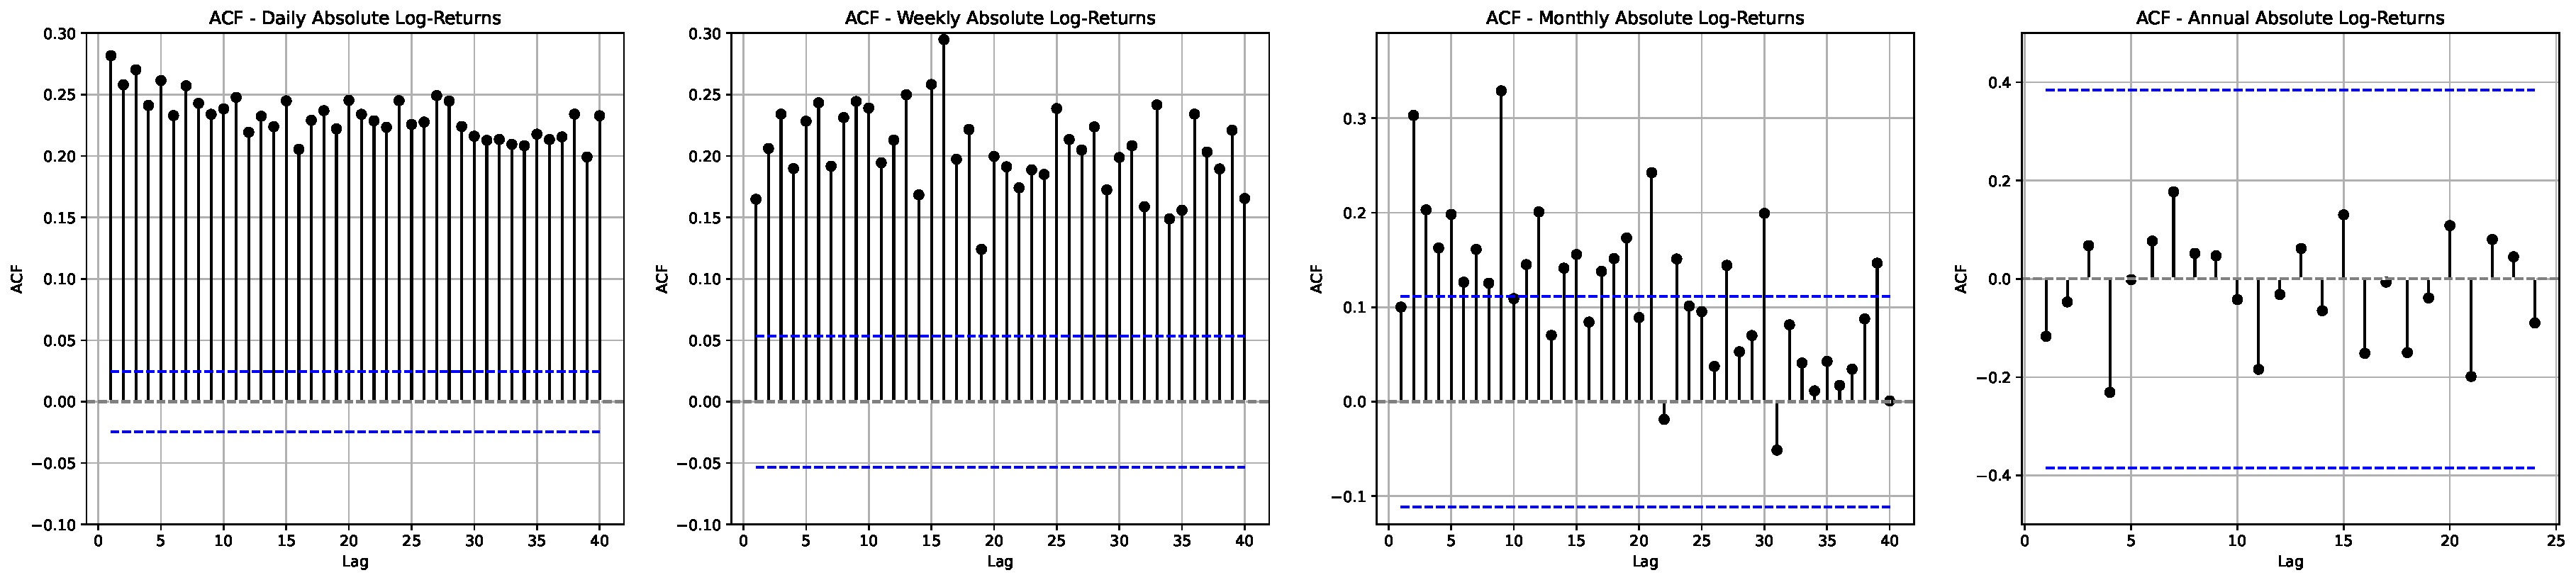
\includegraphics[width=1\textwidth]{Img/Fact7_AbsoluteLogReturns.pdf}
    \caption{Autocorrelations of the daily, weekly and monthly absolute log-returns $r_t$ from the “adjusted closing” of AMZN. Sample: \textbf{01-21-1999} to \textbf{10-16-2024}.
    The \textcolor{blue}{blue dotted} bands represents the confidence intervals (\textbf{Barlett intervals}), $\frac{1}{\sqrt{T}}$ where T is the number of samples.}
    \label{fig:atocorrelation_abs_logreturns}
\end{figure}

\noindent We observe that the autocorrelation is continuous, as indicated by the trendline, 
which aligns with the previous graph. 
Additionally, it becomes apparent that as the time interval changes (from daily to weekly, monthly, and annually) 
the autocorrelation becomes more pronounced between intervals. 
This aligns with the volatility clustering phenomenon discussed earlier. 
This effect occurs because ARCH and GARCH models are sensitive to sampling frequency, 
with their impact being more noticeable at shorter frequencies (daily, weekly) than at longer ones (monthly, annually).

\subsection{Leverage effect}

The leverage effect highlights the negative correlation between an asset's returns and its volatility. 
Figure~\ref{fig:Rolling_std_dev_2} illustrates this phenomenon through cross-correlation values over time. 
The graph clearly shows a strong cross-correlation between the returns $r_{t+j}$ and the squared returns $r_t^2$. 
This is evidenced by most values exceeding the green dashed line, which marks the threshold for the rejection region in the significance test. 
Notably, the majority of values after 2000 are negative, indicating a negative correlation between future returns $R_{t+j}$ and volatility $R^2$.




\begin{figure}[H]
    \centering
    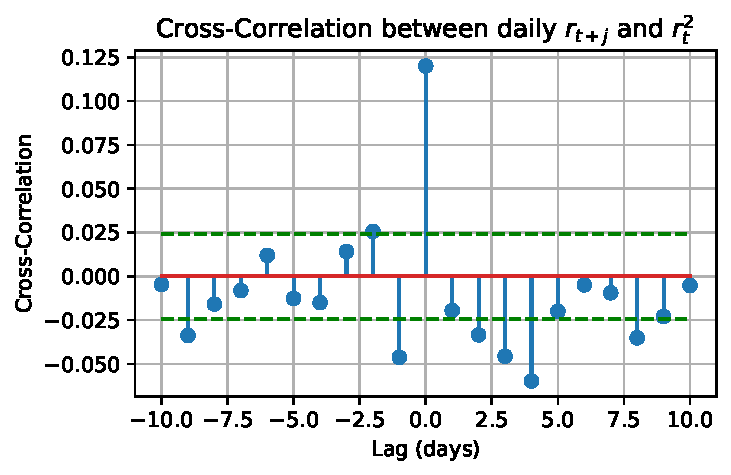
\includegraphics[width=0.5\textwidth]{Img/Fact8_CrossCorr_r_r2.pdf}
    \caption{\textbf{Empirical cross correlation} of daily lagged log-returns and squared daily returns $corr(r_{t+j},r_t^2)$ of AMZN. Sample: \textbf{01-21-1999} to \textbf{10-16-2024}. 
    The green dotted bars are the (asymptotic) bounds for the rejection region a significance test of each cross-correlation. A line above or below the green dashed line represent a significant cross-correlation.}
    \label{fig:Rolling_std_dev_2}
\end{figure}

\begin{figure}[H]
    \begin{minipage}{0.46\textwidth}
        \centering
        \includegraphics[width=1\textwidth]{Img/Fact8.pdf}
        \caption{Time series plot of \textcolor{blue}{AMZN} and \textcolor{orange}{VIX}. Sample: \textbf{01-21-1999} to \textbf{10-16-2024}.}
        \label{fig:Rolling_std_dev_3}
    \end{minipage}
    \centering
    \hspace{0.01\textwidth}
    \begin{minipage}{0.46\textwidth}
        \centering
        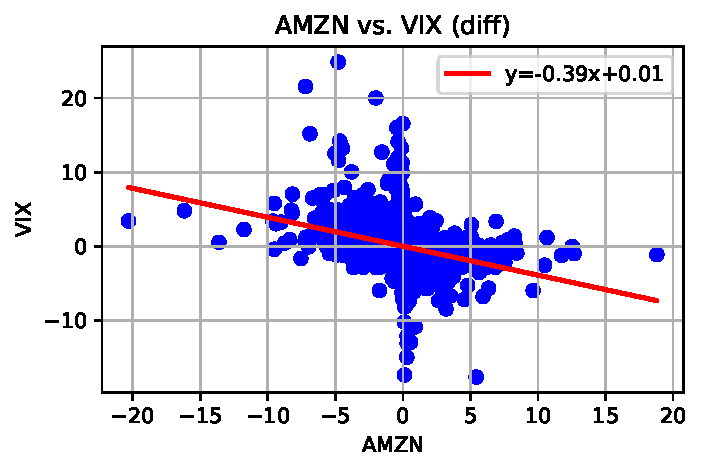
\includegraphics[width=0.8\textwidth]{Img/Fact_8_3AMZN_.pdf}
        \caption{Scatter plot of daily AMZN log-returns against the daily changes of VIX for the same day $t$. 
        Fitted OLS regression line is represented in (\textcolor{red}{red}).
        Sample: \textbf{01-21-1999} to \textbf{10-16-2024}.}
        \label{fig:Rolling_std_dev}
    \end{minipage}
\end{figure}
\noindent The comparison between Amazon's stock and the VIX (Volatility Index) in Figure 15 reveals a negative correlation between the stock and the index. 
This effect is particularly pronounced during the 2008 financial crisis when volatility surged while Amazon's stock experienced a slight decline. 
However, this correlation appears less evident during the dot-com bubble in the early 2000s, as Amazon maintained strong sales during that period. 
Nonetheless, the chart reinforces the negative correlation between Amazon's returns and volatility, 
consistent with the findings from Figure~\ref{fig:Rolling_std_dev_1}.
\appendix
%\section{To go further, CAPM pricing model}
\section{References}
\bibliographystyle{plain}
\bibliography{bibliography} % Do not include the .bib extension


\section{python code}
Notebook starting next page
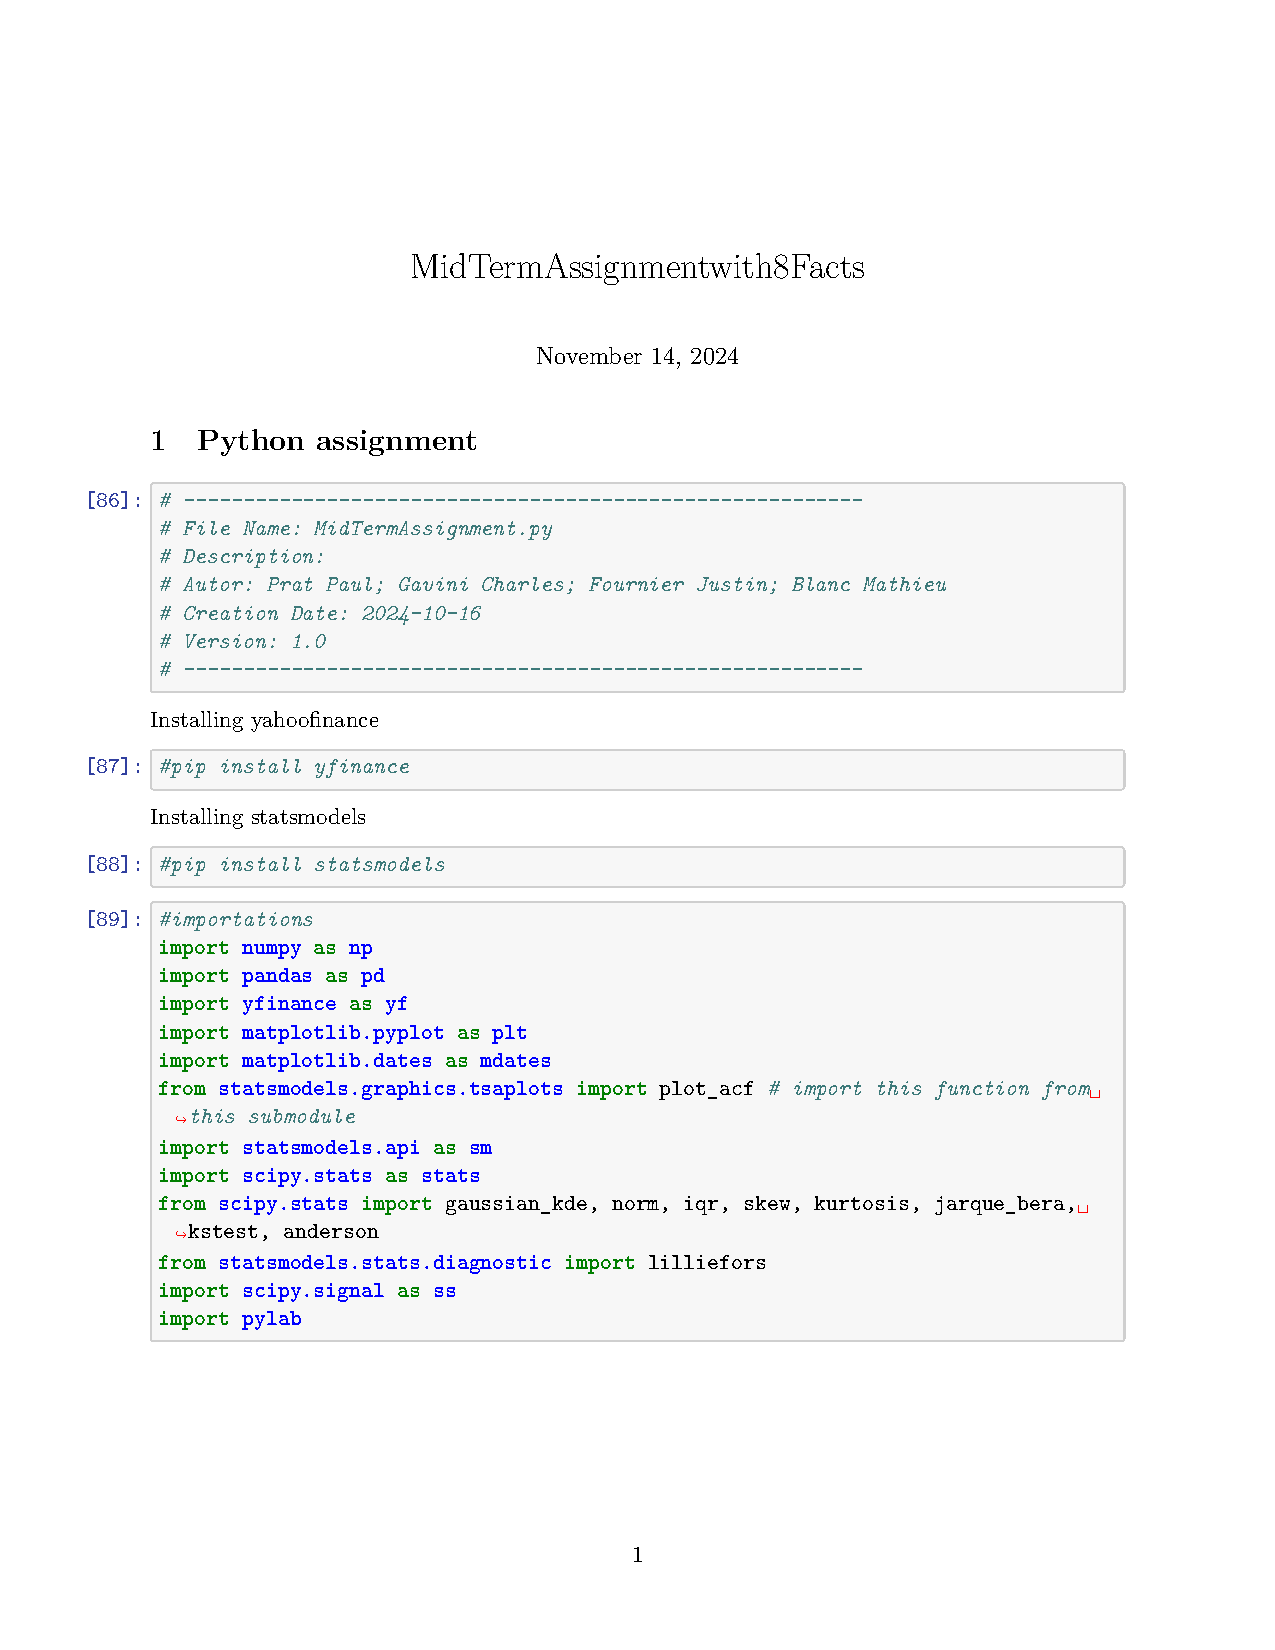
\includepdf[pages=-]{MidTermAssignmentwith8Facts.pdf}
%\documentclass[11pt]{article}

    \usepackage[breakable]{tcolorbox}
    \usepackage{parskip} % Stop auto-indenting (to mimic markdown behaviour)
    

    % Basic figure setup, for now with no caption control since it's done
    % automatically by Pandoc (which extracts ![](path) syntax from Markdown).
    \usepackage{graphicx}
    % Keep aspect ratio if custom image width or height is specified
    \setkeys{Gin}{keepaspectratio}
    % Maintain compatibility with old templates. Remove in nbconvert 6.0
    \let\Oldincludegraphics\includegraphics
    % Ensure that by default, figures have no caption (until we provide a
    % proper Figure object with a Caption API and a way to capture that
    % in the conversion process - todo).
    \usepackage{caption}
    \DeclareCaptionFormat{nocaption}{}
    \captionsetup{format=nocaption,aboveskip=0pt,belowskip=0pt}

    \usepackage{float}
    \floatplacement{figure}{H} % forces figures to be placed at the correct location
    \usepackage{xcolor} % Allow colors to be defined
    \usepackage{enumerate} % Needed for markdown enumerations to work
    \usepackage{geometry} % Used to adjust the document margins
    \usepackage{amsmath} % Equations
    \usepackage{amssymb} % Equations
    \usepackage{textcomp} % defines textquotesingle
    % Hack from http://tex.stackexchange.com/a/47451/13684:
    \AtBeginDocument{%
        \def\PYZsq{\textquotesingle}% Upright quotes in Pygmentized code
    }
    \usepackage{upquote} % Upright quotes for verbatim code
    \usepackage{eurosym} % defines \euro

    \usepackage{iftex}
    \ifPDFTeX
        \usepackage[T1]{fontenc}
        \IfFileExists{alphabeta.sty}{
              \usepackage{alphabeta}
          }{
              \usepackage[mathletters]{ucs}
              \usepackage[utf8x]{inputenc}
          }
    \else
        \usepackage{fontspec}
        \usepackage{unicode-math}
    \fi

    \usepackage{fancyvrb} % verbatim replacement that allows latex
    \usepackage{grffile} % extends the file name processing of package graphics
                         % to support a larger range
    \makeatletter % fix for old versions of grffile with XeLaTeX
    \@ifpackagelater{grffile}{2019/11/01}
    {
      % Do nothing on new versions
    }
    {
      \def\Gread@@xetex#1{%
        \IfFileExists{"\Gin@base".bb}%
        {\Gread@eps{\Gin@base.bb}}%
        {\Gread@@xetex@aux#1}%
      }
    }
    \makeatother
    \usepackage[Export]{adjustbox} % Used to constrain images to a maximum size
    \adjustboxset{max size={0.9\linewidth}{0.9\paperheight}}

    % The hyperref package gives us a pdf with properly built
    % internal navigation ('pdf bookmarks' for the table of contents,
    % internal cross-reference links, web links for URLs, etc.)
    \usepackage{hyperref}
    % The default LaTeX title has an obnoxious amount of whitespace. By default,
    % titling removes some of it. It also provides customization options.
    \usepackage{titling}
    \usepackage{longtable} % longtable support required by pandoc >1.10
    \usepackage{booktabs}  % table support for pandoc > 1.12.2
    \usepackage{array}     % table support for pandoc >= 2.11.3
    \usepackage{calc}      % table minipage width calculation for pandoc >= 2.11.1
    \usepackage[inline]{enumitem} % IRkernel/repr support (it uses the enumerate* environment)
    \usepackage[normalem]{ulem} % ulem is needed to support strikethroughs (\sout)
                                % normalem makes italics be italics, not underlines
    \usepackage{soul}      % strikethrough (\st) support for pandoc >= 3.0.0
    \usepackage{mathrsfs}
    

    
    % Colors for the hyperref package
    \definecolor{urlcolor}{rgb}{0,.145,.698}
    \definecolor{linkcolor}{rgb}{.71,0.21,0.01}
    \definecolor{citecolor}{rgb}{.12,.54,.11}

    % ANSI colors
    \definecolor{ansi-black}{HTML}{3E424D}
    \definecolor{ansi-black-intense}{HTML}{282C36}
    \definecolor{ansi-red}{HTML}{E75C58}
    \definecolor{ansi-red-intense}{HTML}{B22B31}
    \definecolor{ansi-green}{HTML}{00A250}
    \definecolor{ansi-green-intense}{HTML}{007427}
    \definecolor{ansi-yellow}{HTML}{DDB62B}
    \definecolor{ansi-yellow-intense}{HTML}{B27D12}
    \definecolor{ansi-blue}{HTML}{208FFB}
    \definecolor{ansi-blue-intense}{HTML}{0065CA}
    \definecolor{ansi-magenta}{HTML}{D160C4}
    \definecolor{ansi-magenta-intense}{HTML}{A03196}
    \definecolor{ansi-cyan}{HTML}{60C6C8}
    \definecolor{ansi-cyan-intense}{HTML}{258F8F}
    \definecolor{ansi-white}{HTML}{C5C1B4}
    \definecolor{ansi-white-intense}{HTML}{A1A6B2}
    \definecolor{ansi-default-inverse-fg}{HTML}{FFFFFF}
    \definecolor{ansi-default-inverse-bg}{HTML}{000000}

    % common color for the border for error outputs.
    \definecolor{outerrorbackground}{HTML}{FFDFDF}

    % commands and environments needed by pandoc snippets
    % extracted from the output of `pandoc -s`
    \providecommand{\tightlist}{%
      \setlength{\itemsep}{0pt}\setlength{\parskip}{0pt}}
    \DefineVerbatimEnvironment{Highlighting}{Verbatim}{commandchars=\\\{\}}
    % Add ',fontsize=\small' for more characters per line
    \newenvironment{Shaded}{}{}
    \newcommand{\KeywordTok}[1]{\textcolor[rgb]{0.00,0.44,0.13}{\textbf{{#1}}}}
    \newcommand{\DataTypeTok}[1]{\textcolor[rgb]{0.56,0.13,0.00}{{#1}}}
    \newcommand{\DecValTok}[1]{\textcolor[rgb]{0.25,0.63,0.44}{{#1}}}
    \newcommand{\BaseNTok}[1]{\textcolor[rgb]{0.25,0.63,0.44}{{#1}}}
    \newcommand{\FloatTok}[1]{\textcolor[rgb]{0.25,0.63,0.44}{{#1}}}
    \newcommand{\CharTok}[1]{\textcolor[rgb]{0.25,0.44,0.63}{{#1}}}
    \newcommand{\StringTok}[1]{\textcolor[rgb]{0.25,0.44,0.63}{{#1}}}
    \newcommand{\CommentTok}[1]{\textcolor[rgb]{0.38,0.63,0.69}{\textit{{#1}}}}
    \newcommand{\OtherTok}[1]{\textcolor[rgb]{0.00,0.44,0.13}{{#1}}}
    \newcommand{\AlertTok}[1]{\textcolor[rgb]{1.00,0.00,0.00}{\textbf{{#1}}}}
    \newcommand{\FunctionTok}[1]{\textcolor[rgb]{0.02,0.16,0.49}{{#1}}}
    \newcommand{\RegionMarkerTok}[1]{{#1}}
    \newcommand{\ErrorTok}[1]{\textcolor[rgb]{1.00,0.00,0.00}{\textbf{{#1}}}}
    \newcommand{\NormalTok}[1]{{#1}}

    % Additional commands for more recent versions of Pandoc
    \newcommand{\ConstantTok}[1]{\textcolor[rgb]{0.53,0.00,0.00}{{#1}}}
    \newcommand{\SpecialCharTok}[1]{\textcolor[rgb]{0.25,0.44,0.63}{{#1}}}
    \newcommand{\VerbatimStringTok}[1]{\textcolor[rgb]{0.25,0.44,0.63}{{#1}}}
    \newcommand{\SpecialStringTok}[1]{\textcolor[rgb]{0.73,0.40,0.53}{{#1}}}
    \newcommand{\ImportTok}[1]{{#1}}
    \newcommand{\DocumentationTok}[1]{\textcolor[rgb]{0.73,0.13,0.13}{\textit{{#1}}}}
    \newcommand{\AnnotationTok}[1]{\textcolor[rgb]{0.38,0.63,0.69}{\textbf{\textit{{#1}}}}}
    \newcommand{\CommentVarTok}[1]{\textcolor[rgb]{0.38,0.63,0.69}{\textbf{\textit{{#1}}}}}
    \newcommand{\VariableTok}[1]{\textcolor[rgb]{0.10,0.09,0.49}{{#1}}}
    \newcommand{\ControlFlowTok}[1]{\textcolor[rgb]{0.00,0.44,0.13}{\textbf{{#1}}}}
    \newcommand{\OperatorTok}[1]{\textcolor[rgb]{0.40,0.40,0.40}{{#1}}}
    \newcommand{\BuiltInTok}[1]{{#1}}
    \newcommand{\ExtensionTok}[1]{{#1}}
    \newcommand{\PreprocessorTok}[1]{\textcolor[rgb]{0.74,0.48,0.00}{{#1}}}
    \newcommand{\AttributeTok}[1]{\textcolor[rgb]{0.49,0.56,0.16}{{#1}}}
    \newcommand{\InformationTok}[1]{\textcolor[rgb]{0.38,0.63,0.69}{\textbf{\textit{{#1}}}}}
    \newcommand{\WarningTok}[1]{\textcolor[rgb]{0.38,0.63,0.69}{\textbf{\textit{{#1}}}}}


    % Define a nice break command that doesn't care if a line doesn't already
    % exist.
    \def\br{\hspace*{\fill} \\* }
    % Math Jax compatibility definitions
    \def\gt{>}
    \def\lt{<}
    \let\Oldtex\TeX
    \let\Oldlatex\LaTeX
    \renewcommand{\TeX}{\textrm{\Oldtex}}
    \renewcommand{\LaTeX}{\textrm{\Oldlatex}}
    % Document parameters
    % Document title
    \title{MidTermAssignmentwith8Facts}
    
    
    
    
    
    
    
% Pygments definitions
\makeatletter
\def\PY@reset{\let\PY@it=\relax \let\PY@bf=\relax%
    \let\PY@ul=\relax \let\PY@tc=\relax%
    \let\PY@bc=\relax \let\PY@ff=\relax}
\def\PY@tok#1{\csname PY@tok@#1\endcsname}
\def\PY@toks#1+{\ifx\relax#1\empty\else%
    \PY@tok{#1}\expandafter\PY@toks\fi}
\def\PY@do#1{\PY@bc{\PY@tc{\PY@ul{%
    \PY@it{\PY@bf{\PY@ff{#1}}}}}}}
\def\PY#1#2{\PY@reset\PY@toks#1+\relax+\PY@do{#2}}

\@namedef{PY@tok@w}{\def\PY@tc##1{\textcolor[rgb]{0.73,0.73,0.73}{##1}}}
\@namedef{PY@tok@c}{\let\PY@it=\textit\def\PY@tc##1{\textcolor[rgb]{0.24,0.48,0.48}{##1}}}
\@namedef{PY@tok@cp}{\def\PY@tc##1{\textcolor[rgb]{0.61,0.40,0.00}{##1}}}
\@namedef{PY@tok@k}{\let\PY@bf=\textbf\def\PY@tc##1{\textcolor[rgb]{0.00,0.50,0.00}{##1}}}
\@namedef{PY@tok@kp}{\def\PY@tc##1{\textcolor[rgb]{0.00,0.50,0.00}{##1}}}
\@namedef{PY@tok@kt}{\def\PY@tc##1{\textcolor[rgb]{0.69,0.00,0.25}{##1}}}
\@namedef{PY@tok@o}{\def\PY@tc##1{\textcolor[rgb]{0.40,0.40,0.40}{##1}}}
\@namedef{PY@tok@ow}{\let\PY@bf=\textbf\def\PY@tc##1{\textcolor[rgb]{0.67,0.13,1.00}{##1}}}
\@namedef{PY@tok@nb}{\def\PY@tc##1{\textcolor[rgb]{0.00,0.50,0.00}{##1}}}
\@namedef{PY@tok@nf}{\def\PY@tc##1{\textcolor[rgb]{0.00,0.00,1.00}{##1}}}
\@namedef{PY@tok@nc}{\let\PY@bf=\textbf\def\PY@tc##1{\textcolor[rgb]{0.00,0.00,1.00}{##1}}}
\@namedef{PY@tok@nn}{\let\PY@bf=\textbf\def\PY@tc##1{\textcolor[rgb]{0.00,0.00,1.00}{##1}}}
\@namedef{PY@tok@ne}{\let\PY@bf=\textbf\def\PY@tc##1{\textcolor[rgb]{0.80,0.25,0.22}{##1}}}
\@namedef{PY@tok@nv}{\def\PY@tc##1{\textcolor[rgb]{0.10,0.09,0.49}{##1}}}
\@namedef{PY@tok@no}{\def\PY@tc##1{\textcolor[rgb]{0.53,0.00,0.00}{##1}}}
\@namedef{PY@tok@nl}{\def\PY@tc##1{\textcolor[rgb]{0.46,0.46,0.00}{##1}}}
\@namedef{PY@tok@ni}{\let\PY@bf=\textbf\def\PY@tc##1{\textcolor[rgb]{0.44,0.44,0.44}{##1}}}
\@namedef{PY@tok@na}{\def\PY@tc##1{\textcolor[rgb]{0.41,0.47,0.13}{##1}}}
\@namedef{PY@tok@nt}{\let\PY@bf=\textbf\def\PY@tc##1{\textcolor[rgb]{0.00,0.50,0.00}{##1}}}
\@namedef{PY@tok@nd}{\def\PY@tc##1{\textcolor[rgb]{0.67,0.13,1.00}{##1}}}
\@namedef{PY@tok@s}{\def\PY@tc##1{\textcolor[rgb]{0.73,0.13,0.13}{##1}}}
\@namedef{PY@tok@sd}{\let\PY@it=\textit\def\PY@tc##1{\textcolor[rgb]{0.73,0.13,0.13}{##1}}}
\@namedef{PY@tok@si}{\let\PY@bf=\textbf\def\PY@tc##1{\textcolor[rgb]{0.64,0.35,0.47}{##1}}}
\@namedef{PY@tok@se}{\let\PY@bf=\textbf\def\PY@tc##1{\textcolor[rgb]{0.67,0.36,0.12}{##1}}}
\@namedef{PY@tok@sr}{\def\PY@tc##1{\textcolor[rgb]{0.64,0.35,0.47}{##1}}}
\@namedef{PY@tok@ss}{\def\PY@tc##1{\textcolor[rgb]{0.10,0.09,0.49}{##1}}}
\@namedef{PY@tok@sx}{\def\PY@tc##1{\textcolor[rgb]{0.00,0.50,0.00}{##1}}}
\@namedef{PY@tok@m}{\def\PY@tc##1{\textcolor[rgb]{0.40,0.40,0.40}{##1}}}
\@namedef{PY@tok@gh}{\let\PY@bf=\textbf\def\PY@tc##1{\textcolor[rgb]{0.00,0.00,0.50}{##1}}}
\@namedef{PY@tok@gu}{\let\PY@bf=\textbf\def\PY@tc##1{\textcolor[rgb]{0.50,0.00,0.50}{##1}}}
\@namedef{PY@tok@gd}{\def\PY@tc##1{\textcolor[rgb]{0.63,0.00,0.00}{##1}}}
\@namedef{PY@tok@gi}{\def\PY@tc##1{\textcolor[rgb]{0.00,0.52,0.00}{##1}}}
\@namedef{PY@tok@gr}{\def\PY@tc##1{\textcolor[rgb]{0.89,0.00,0.00}{##1}}}
\@namedef{PY@tok@ge}{\let\PY@it=\textit}
\@namedef{PY@tok@gs}{\let\PY@bf=\textbf}
\@namedef{PY@tok@gp}{\let\PY@bf=\textbf\def\PY@tc##1{\textcolor[rgb]{0.00,0.00,0.50}{##1}}}
\@namedef{PY@tok@go}{\def\PY@tc##1{\textcolor[rgb]{0.44,0.44,0.44}{##1}}}
\@namedef{PY@tok@gt}{\def\PY@tc##1{\textcolor[rgb]{0.00,0.27,0.87}{##1}}}
\@namedef{PY@tok@err}{\def\PY@bc##1{{\setlength{\fboxsep}{\string -\fboxrule}\fcolorbox[rgb]{1.00,0.00,0.00}{1,1,1}{\strut ##1}}}}
\@namedef{PY@tok@kc}{\let\PY@bf=\textbf\def\PY@tc##1{\textcolor[rgb]{0.00,0.50,0.00}{##1}}}
\@namedef{PY@tok@kd}{\let\PY@bf=\textbf\def\PY@tc##1{\textcolor[rgb]{0.00,0.50,0.00}{##1}}}
\@namedef{PY@tok@kn}{\let\PY@bf=\textbf\def\PY@tc##1{\textcolor[rgb]{0.00,0.50,0.00}{##1}}}
\@namedef{PY@tok@kr}{\let\PY@bf=\textbf\def\PY@tc##1{\textcolor[rgb]{0.00,0.50,0.00}{##1}}}
\@namedef{PY@tok@bp}{\def\PY@tc##1{\textcolor[rgb]{0.00,0.50,0.00}{##1}}}
\@namedef{PY@tok@fm}{\def\PY@tc##1{\textcolor[rgb]{0.00,0.00,1.00}{##1}}}
\@namedef{PY@tok@vc}{\def\PY@tc##1{\textcolor[rgb]{0.10,0.09,0.49}{##1}}}
\@namedef{PY@tok@vg}{\def\PY@tc##1{\textcolor[rgb]{0.10,0.09,0.49}{##1}}}
\@namedef{PY@tok@vi}{\def\PY@tc##1{\textcolor[rgb]{0.10,0.09,0.49}{##1}}}
\@namedef{PY@tok@vm}{\def\PY@tc##1{\textcolor[rgb]{0.10,0.09,0.49}{##1}}}
\@namedef{PY@tok@sa}{\def\PY@tc##1{\textcolor[rgb]{0.73,0.13,0.13}{##1}}}
\@namedef{PY@tok@sb}{\def\PY@tc##1{\textcolor[rgb]{0.73,0.13,0.13}{##1}}}
\@namedef{PY@tok@sc}{\def\PY@tc##1{\textcolor[rgb]{0.73,0.13,0.13}{##1}}}
\@namedef{PY@tok@dl}{\def\PY@tc##1{\textcolor[rgb]{0.73,0.13,0.13}{##1}}}
\@namedef{PY@tok@s2}{\def\PY@tc##1{\textcolor[rgb]{0.73,0.13,0.13}{##1}}}
\@namedef{PY@tok@sh}{\def\PY@tc##1{\textcolor[rgb]{0.73,0.13,0.13}{##1}}}
\@namedef{PY@tok@s1}{\def\PY@tc##1{\textcolor[rgb]{0.73,0.13,0.13}{##1}}}
\@namedef{PY@tok@mb}{\def\PY@tc##1{\textcolor[rgb]{0.40,0.40,0.40}{##1}}}
\@namedef{PY@tok@mf}{\def\PY@tc##1{\textcolor[rgb]{0.40,0.40,0.40}{##1}}}
\@namedef{PY@tok@mh}{\def\PY@tc##1{\textcolor[rgb]{0.40,0.40,0.40}{##1}}}
\@namedef{PY@tok@mi}{\def\PY@tc##1{\textcolor[rgb]{0.40,0.40,0.40}{##1}}}
\@namedef{PY@tok@il}{\def\PY@tc##1{\textcolor[rgb]{0.40,0.40,0.40}{##1}}}
\@namedef{PY@tok@mo}{\def\PY@tc##1{\textcolor[rgb]{0.40,0.40,0.40}{##1}}}
\@namedef{PY@tok@ch}{\let\PY@it=\textit\def\PY@tc##1{\textcolor[rgb]{0.24,0.48,0.48}{##1}}}
\@namedef{PY@tok@cm}{\let\PY@it=\textit\def\PY@tc##1{\textcolor[rgb]{0.24,0.48,0.48}{##1}}}
\@namedef{PY@tok@cpf}{\let\PY@it=\textit\def\PY@tc##1{\textcolor[rgb]{0.24,0.48,0.48}{##1}}}
\@namedef{PY@tok@c1}{\let\PY@it=\textit\def\PY@tc##1{\textcolor[rgb]{0.24,0.48,0.48}{##1}}}
\@namedef{PY@tok@cs}{\let\PY@it=\textit\def\PY@tc##1{\textcolor[rgb]{0.24,0.48,0.48}{##1}}}

\def\PYZbs{\char`\\}
\def\PYZus{\char`\_}
\def\PYZob{\char`\{}
\def\PYZcb{\char`\}}
\def\PYZca{\char`\^}
\def\PYZam{\char`\&}
\def\PYZlt{\char`\<}
\def\PYZgt{\char`\>}
\def\PYZsh{\char`\#}
\def\PYZpc{\char`\%}
\def\PYZdl{\char`\$}
\def\PYZhy{\char`\-}
\def\PYZsq{\char`\'}
\def\PYZdq{\char`\"}
\def\PYZti{\char`\~}
% for compatibility with earlier versions
\def\PYZat{@}
\def\PYZlb{[}
\def\PYZrb{]}
\makeatother


    % For linebreaks inside Verbatim environment from package fancyvrb.
    \makeatletter
        \newbox\Wrappedcontinuationbox
        \newbox\Wrappedvisiblespacebox
        \newcommand*\Wrappedvisiblespace {\textcolor{red}{\textvisiblespace}}
        \newcommand*\Wrappedcontinuationsymbol {\textcolor{red}{\llap{\tiny$\m@th\hookrightarrow$}}}
        \newcommand*\Wrappedcontinuationindent {3ex }
        \newcommand*\Wrappedafterbreak {\kern\Wrappedcontinuationindent\copy\Wrappedcontinuationbox}
        % Take advantage of the already applied Pygments mark-up to insert
        % potential linebreaks for TeX processing.
        %        {, <, #, %, $, ' and ": go to next line.
        %        _, }, ^, &, >, - and ~: stay at end of broken line.
        % Use of \textquotesingle for straight quote.
        \newcommand*\Wrappedbreaksatspecials {%
            \def\PYGZus{\discretionary{\char`\_}{\Wrappedafterbreak}{\char`\_}}%
            \def\PYGZob{\discretionary{}{\Wrappedafterbreak\char`\{}{\char`\{}}%
            \def\PYGZcb{\discretionary{\char`\}}{\Wrappedafterbreak}{\char`\}}}%
            \def\PYGZca{\discretionary{\char`\^}{\Wrappedafterbreak}{\char`\^}}%
            \def\PYGZam{\discretionary{\char`\&}{\Wrappedafterbreak}{\char`\&}}%
            \def\PYGZlt{\discretionary{}{\Wrappedafterbreak\char`\<}{\char`\<}}%
            \def\PYGZgt{\discretionary{\char`\>}{\Wrappedafterbreak}{\char`\>}}%
            \def\PYGZsh{\discretionary{}{\Wrappedafterbreak\char`\#}{\char`\#}}%
            \def\PYGZpc{\discretionary{}{\Wrappedafterbreak\char`\%}{\char`\%}}%
            \def\PYGZdl{\discretionary{}{\Wrappedafterbreak\char`\$}{\char`\$}}%
            \def\PYGZhy{\discretionary{\char`\-}{\Wrappedafterbreak}{\char`\-}}%
            \def\PYGZsq{\discretionary{}{\Wrappedafterbreak\textquotesingle}{\textquotesingle}}%
            \def\PYGZdq{\discretionary{}{\Wrappedafterbreak\char`\"}{\char`\"}}%
            \def\PYGZti{\discretionary{\char`\~}{\Wrappedafterbreak}{\char`\~}}%
        }
        % Some characters . , ; ? ! / are not pygmentized.
        % This macro makes them "active" and they will insert potential linebreaks
        \newcommand*\Wrappedbreaksatpunct {%
            \lccode`\~`\.\lowercase{\def~}{\discretionary{\hbox{\char`\.}}{\Wrappedafterbreak}{\hbox{\char`\.}}}%
            \lccode`\~`\,\lowercase{\def~}{\discretionary{\hbox{\char`\,}}{\Wrappedafterbreak}{\hbox{\char`\,}}}%
            \lccode`\~`\;\lowercase{\def~}{\discretionary{\hbox{\char`\;}}{\Wrappedafterbreak}{\hbox{\char`\;}}}%
            \lccode`\~`\:\lowercase{\def~}{\discretionary{\hbox{\char`\:}}{\Wrappedafterbreak}{\hbox{\char`\:}}}%
            \lccode`\~`\?\lowercase{\def~}{\discretionary{\hbox{\char`\?}}{\Wrappedafterbreak}{\hbox{\char`\?}}}%
            \lccode`\~`\!\lowercase{\def~}{\discretionary{\hbox{\char`\!}}{\Wrappedafterbreak}{\hbox{\char`\!}}}%
            \lccode`\~`\/\lowercase{\def~}{\discretionary{\hbox{\char`\/}}{\Wrappedafterbreak}{\hbox{\char`\/}}}%
            \catcode`\.\active
            \catcode`\,\active
            \catcode`\;\active
            \catcode`\:\active
            \catcode`\?\active
            \catcode`\!\active
            \catcode`\/\active
            \lccode`\~`\~
        }
    \makeatother

    \let\OriginalVerbatim=\Verbatim
    \makeatletter
    \renewcommand{\Verbatim}[1][1]{%
        %\parskip\z@skip
        \sbox\Wrappedcontinuationbox {\Wrappedcontinuationsymbol}%
        \sbox\Wrappedvisiblespacebox {\FV@SetupFont\Wrappedvisiblespace}%
        \def\FancyVerbFormatLine ##1{\hsize\linewidth
            \vtop{\raggedright\hyphenpenalty\z@\exhyphenpenalty\z@
                \doublehyphendemerits\z@\finalhyphendemerits\z@
                \strut ##1\strut}%
        }%
        % If the linebreak is at a space, the latter will be displayed as visible
        % space at end of first line, and a continuation symbol starts next line.
        % Stretch/shrink are however usually zero for typewriter font.
        \def\FV@Space {%
            \nobreak\hskip\z@ plus\fontdimen3\font minus\fontdimen4\font
            \discretionary{\copy\Wrappedvisiblespacebox}{\Wrappedafterbreak}
            {\kern\fontdimen2\font}%
        }%

        % Allow breaks at special characters using \PYG... macros.
        \Wrappedbreaksatspecials
        % Breaks at punctuation characters . , ; ? ! and / need catcode=\active
        \OriginalVerbatim[#1,codes*=\Wrappedbreaksatpunct]%
    }
    \makeatother

    % Exact colors from NB
    \definecolor{incolor}{HTML}{303F9F}
    \definecolor{outcolor}{HTML}{D84315}
    \definecolor{cellborder}{HTML}{CFCFCF}
    \definecolor{cellbackground}{HTML}{F7F7F7}

    % prompt
    \makeatletter
    \newcommand{\boxspacing}{\kern\kvtcb@left@rule\kern\kvtcb@boxsep}
    \makeatother
    \newcommand{\prompt}[4]{
        {\ttfamily\llap{{\color{#2}[#3]:\hspace{3pt}#4}}\vspace{-\baselineskip}}
    }
    

    
    % Prevent overflowing lines due to hard-to-break entities
    \sloppy
    % Setup hyperref package
    \hypersetup{
      breaklinks=true,  % so long urls are correctly broken across lines
      colorlinks=true,
      urlcolor=urlcolor,
      linkcolor=linkcolor,
      citecolor=citecolor,
      }
    % Slightly bigger margins than the latex defaults
    
    \geometry{verbose,tmargin=1in,bmargin=1in,lmargin=1in,rmargin=1in}
    
    

\begin{document}
    
    \maketitle
    
    

    
    

    \section{\texorpdfstring{\textbf{Python
assignment}}{Python assignment}}\label{python-assignment}

    \begin{tcolorbox}[breakable, size=fbox, boxrule=1pt, pad at break*=1mm,colback=cellbackground, colframe=cellborder]
\prompt{In}{incolor}{86}{\boxspacing}
\begin{Verbatim}[commandchars=\\\{\}]
\PY{c+c1}{\PYZsh{} \PYZhy{}\PYZhy{}\PYZhy{}\PYZhy{}\PYZhy{}\PYZhy{}\PYZhy{}\PYZhy{}\PYZhy{}\PYZhy{}\PYZhy{}\PYZhy{}\PYZhy{}\PYZhy{}\PYZhy{}\PYZhy{}\PYZhy{}\PYZhy{}\PYZhy{}\PYZhy{}\PYZhy{}\PYZhy{}\PYZhy{}\PYZhy{}\PYZhy{}\PYZhy{}\PYZhy{}\PYZhy{}\PYZhy{}\PYZhy{}\PYZhy{}\PYZhy{}\PYZhy{}\PYZhy{}\PYZhy{}\PYZhy{}\PYZhy{}\PYZhy{}\PYZhy{}\PYZhy{}\PYZhy{}\PYZhy{}\PYZhy{}\PYZhy{}\PYZhy{}\PYZhy{}\PYZhy{}\PYZhy{}\PYZhy{}\PYZhy{}\PYZhy{}\PYZhy{}\PYZhy{}\PYZhy{}\PYZhy{}\PYZhy{}\PYZhy{}}
\PY{c+c1}{\PYZsh{} File Name: MidTermAssignment.py}
\PY{c+c1}{\PYZsh{} Description: }
\PY{c+c1}{\PYZsh{} Autor: Prat Paul; Gavini Charles; Fournier Justin; Blanc Mathieu}
\PY{c+c1}{\PYZsh{} Creation Date: 2024\PYZhy{}10\PYZhy{}16}
\PY{c+c1}{\PYZsh{} Version: 1.0}
\PY{c+c1}{\PYZsh{} \PYZhy{}\PYZhy{}\PYZhy{}\PYZhy{}\PYZhy{}\PYZhy{}\PYZhy{}\PYZhy{}\PYZhy{}\PYZhy{}\PYZhy{}\PYZhy{}\PYZhy{}\PYZhy{}\PYZhy{}\PYZhy{}\PYZhy{}\PYZhy{}\PYZhy{}\PYZhy{}\PYZhy{}\PYZhy{}\PYZhy{}\PYZhy{}\PYZhy{}\PYZhy{}\PYZhy{}\PYZhy{}\PYZhy{}\PYZhy{}\PYZhy{}\PYZhy{}\PYZhy{}\PYZhy{}\PYZhy{}\PYZhy{}\PYZhy{}\PYZhy{}\PYZhy{}\PYZhy{}\PYZhy{}\PYZhy{}\PYZhy{}\PYZhy{}\PYZhy{}\PYZhy{}\PYZhy{}\PYZhy{}\PYZhy{}\PYZhy{}\PYZhy{}\PYZhy{}\PYZhy{}\PYZhy{}\PYZhy{}\PYZhy{}\PYZhy{}}
\end{Verbatim}
\end{tcolorbox}

    Installing yahoofinance

    \begin{tcolorbox}[breakable, size=fbox, boxrule=1pt, pad at break*=1mm,colback=cellbackground, colframe=cellborder]
\prompt{In}{incolor}{87}{\boxspacing}
\begin{Verbatim}[commandchars=\\\{\}]
\PY{c+c1}{\PYZsh{}pip install yfinance}
\end{Verbatim}
\end{tcolorbox}

    Installing statsmodels

    \begin{tcolorbox}[breakable, size=fbox, boxrule=1pt, pad at break*=1mm,colback=cellbackground, colframe=cellborder]
\prompt{In}{incolor}{88}{\boxspacing}
\begin{Verbatim}[commandchars=\\\{\}]
\PY{c+c1}{\PYZsh{}pip install statsmodels}
\end{Verbatim}
\end{tcolorbox}

    \begin{tcolorbox}[breakable, size=fbox, boxrule=1pt, pad at break*=1mm,colback=cellbackground, colframe=cellborder]
\prompt{In}{incolor}{89}{\boxspacing}
\begin{Verbatim}[commandchars=\\\{\}]
\PY{c+c1}{\PYZsh{}importations}
\PY{k+kn}{import} \PY{n+nn}{numpy} \PY{k}{as} \PY{n+nn}{np}
\PY{k+kn}{import} \PY{n+nn}{pandas} \PY{k}{as} \PY{n+nn}{pd}
\PY{k+kn}{import} \PY{n+nn}{yfinance} \PY{k}{as} \PY{n+nn}{yf}
\PY{k+kn}{import} \PY{n+nn}{matplotlib}\PY{n+nn}{.}\PY{n+nn}{pyplot} \PY{k}{as} \PY{n+nn}{plt}
\PY{k+kn}{import} \PY{n+nn}{matplotlib}\PY{n+nn}{.}\PY{n+nn}{dates} \PY{k}{as} \PY{n+nn}{mdates}
\PY{k+kn}{from} \PY{n+nn}{statsmodels}\PY{n+nn}{.}\PY{n+nn}{graphics}\PY{n+nn}{.}\PY{n+nn}{tsaplots} \PY{k+kn}{import} \PY{n}{plot\PYZus{}acf} \PY{c+c1}{\PYZsh{} import this function from this submodule}
\PY{k+kn}{import} \PY{n+nn}{statsmodels}\PY{n+nn}{.}\PY{n+nn}{api} \PY{k}{as} \PY{n+nn}{sm}
\PY{k+kn}{import} \PY{n+nn}{scipy}\PY{n+nn}{.}\PY{n+nn}{stats} \PY{k}{as} \PY{n+nn}{stats}
\PY{k+kn}{from} \PY{n+nn}{scipy}\PY{n+nn}{.}\PY{n+nn}{stats} \PY{k+kn}{import} \PY{n}{gaussian\PYZus{}kde}\PY{p}{,} \PY{n}{norm}\PY{p}{,} \PY{n}{iqr}\PY{p}{,} \PY{n}{skew}\PY{p}{,} \PY{n}{kurtosis}\PY{p}{,} \PY{n}{jarque\PYZus{}bera}\PY{p}{,} \PY{n}{kstest}\PY{p}{,} \PY{n}{anderson}
\PY{k+kn}{from} \PY{n+nn}{statsmodels}\PY{n+nn}{.}\PY{n+nn}{stats}\PY{n+nn}{.}\PY{n+nn}{diagnostic} \PY{k+kn}{import} \PY{n}{lilliefors}
\PY{k+kn}{import} \PY{n+nn}{scipy}\PY{n+nn}{.}\PY{n+nn}{signal} \PY{k}{as} \PY{n+nn}{ss}
\PY{k+kn}{import} \PY{n+nn}{pylab}
\end{Verbatim}
\end{tcolorbox}

    \section{\texorpdfstring{\emph{First pandas dataframe of Amazon
stocks}}{First pandas dataframe of Amazon stocks}}\label{first-pandas-dataframe-of-amazon-stocks}

    \begin{tcolorbox}[breakable, size=fbox, boxrule=1pt, pad at break*=1mm,colback=cellbackground, colframe=cellborder]
\prompt{In}{incolor}{90}{\boxspacing}
\begin{Verbatim}[commandchars=\\\{\}]
\PY{c+c1}{\PYZsh{} Importing Amazon stock from yahoo finance}
\PY{n}{Amazon} \PY{o}{=} \PY{n}{yf}\PY{o}{.}\PY{n}{download}\PY{p}{(}\PY{l+s+s2}{\PYZdq{}}\PY{l+s+s2}{AMZN}\PY{l+s+s2}{\PYZdq{}}\PY{p}{,} \PY{n}{start}\PY{o}{=}\PY{l+s+s2}{\PYZdq{}}\PY{l+s+s2}{1999\PYZhy{}01\PYZhy{}21}\PY{l+s+s2}{\PYZdq{}}\PY{p}{,} \PY{n}{end}\PY{o}{=}\PY{l+s+s2}{\PYZdq{}}\PY{l+s+s2}{2024\PYZhy{}10\PYZhy{}16}\PY{l+s+s2}{\PYZdq{}}\PY{p}{)}
\PY{n}{Amazon}\PY{o}{.}\PY{n}{head}\PY{p}{(}\PY{p}{)}
\end{Verbatim}
\end{tcolorbox}

    \begin{Verbatim}[commandchars=\\\{\}]
[*********************100\%***********************]  1 of 1 completed
    \end{Verbatim}

            \begin{tcolorbox}[breakable, size=fbox, boxrule=.5pt, pad at break*=1mm, opacityfill=0]
\prompt{Out}{outcolor}{90}{\boxspacing}
\begin{Verbatim}[commandchars=\\\{\}]
                Open      High       Low     Close  Adj Close     Volume
Date
1999-01-21  2.612500  2.759375  2.314063  2.650000   2.650000  940964000
1999-01-22  2.487500  3.146875  2.468750  3.075000   3.075000  875316000
1999-01-25  3.037500  3.084375  2.750000  2.809375   2.809375  546476000
1999-01-26  2.815625  3.031250  2.765625  2.877344   2.877344  490696000
1999-01-27  3.353125  3.493750  3.000000  3.140625   3.140625  700452000
\end{Verbatim}
\end{tcolorbox}
        
    \begin{tcolorbox}[breakable, size=fbox, boxrule=1pt, pad at break*=1mm,colback=cellbackground, colframe=cellborder]
\prompt{In}{incolor}{91}{\boxspacing}
\begin{Verbatim}[commandchars=\\\{\}]
\PY{c+c1}{\PYZsh{}pip install perfplot}
\end{Verbatim}
\end{tcolorbox}

    \begin{tcolorbox}[breakable, size=fbox, boxrule=1pt, pad at break*=1mm,colback=cellbackground, colframe=cellborder]
\prompt{In}{incolor}{92}{\boxspacing}
\begin{Verbatim}[commandchars=\\\{\}]
\PY{n}{latex\PYZus{}table} \PY{o}{=} \PY{n}{Amazon}\PY{o}{.}\PY{n}{head}\PY{p}{(}\PY{p}{)}\PY{o}{.}\PY{n}{to\PYZus{}latex}\PY{p}{(}\PY{n}{index}\PY{o}{=}\PY{k+kc}{True}\PY{p}{)}
\PY{k}{with} \PY{n+nb}{open}\PY{p}{(}\PY{l+s+s2}{\PYZdq{}}\PY{l+s+s2}{Latex/table.tex}\PY{l+s+s2}{\PYZdq{}}\PY{p}{,} \PY{l+s+s2}{\PYZdq{}}\PY{l+s+s2}{w}\PY{l+s+s2}{\PYZdq{}}\PY{p}{)} \PY{k}{as} \PY{n}{file}\PY{p}{:}
    \PY{n}{file}\PY{o}{.}\PY{n}{write}\PY{p}{(}\PY{n}{latex\PYZus{}table}\PY{p}{)}
\end{Verbatim}
\end{tcolorbox}

    \begin{Verbatim}[commandchars=\\\{\}]
/var/folders/5r/ft807c7n1ngd3fpt2\_gwsg0m0000gn/T/ipykernel\_78356/3304008134.py:1
: FutureWarning: In future versions `DataFrame.to\_latex` is expected to utilise
the base implementation of `Styler.to\_latex` for formatting and rendering. The
arguments signature may therefore change. It is recommended instead to use
`DataFrame.style.to\_latex` which also contains additional functionality.
  latex\_table = Amazon.head().to\_latex(index=True)
    \end{Verbatim}

    \section{\texorpdfstring{\emph{Cheking if timestamp is 25
years}}{Cheking if timestamp is 25 years}}\label{cheking-if-timestamp-is-25-years}

    \begin{tcolorbox}[breakable, size=fbox, boxrule=1pt, pad at break*=1mm,colback=cellbackground, colframe=cellborder]
\prompt{In}{incolor}{93}{\boxspacing}
\begin{Verbatim}[commandchars=\\\{\}]
\PY{n+nb}{print}\PY{p}{(}\PY{l+s+s1}{\PYZsq{}}\PY{l+s+s1}{Amazon data range is: }\PY{l+s+s1}{\PYZsq{}}\PY{p}{,}\PY{n}{Amazon}\PY{o}{.}\PY{n}{index}\PY{p}{[}\PY{l+m+mi}{0}\PY{p}{]}\PY{p}{,}\PY{n}{Amazon}\PY{o}{.}\PY{n}{index}\PY{p}{[}\PY{o}{\PYZhy{}}\PY{l+m+mi}{1}\PY{p}{]}\PY{p}{)}

\PY{c+c1}{\PYZsh{}trying to find gaps}

\PY{c+c1}{\PYZsh{}First create a dataframe for a fullrange of our index, without any gap with the following formula: }
\PY{n}{full\PYZus{}range} \PY{o}{=} \PY{n}{pd}\PY{o}{.}\PY{n}{date\PYZus{}range}\PY{p}{(}\PY{n}{start}\PY{o}{=}\PY{n}{Amazon}\PY{o}{.}\PY{n}{index}\PY{o}{.}\PY{n}{min}\PY{p}{(}\PY{p}{)}\PY{p}{,} \PY{n}{end}\PY{o}{=}\PY{n}{Amazon}\PY{o}{.}\PY{n}{index}\PY{o}{.}\PY{n}{max}\PY{p}{(}\PY{p}{)}\PY{p}{,} \PY{n}{freq}\PY{o}{=}\PY{l+s+s1}{\PYZsq{}}\PY{l+s+s1}{B}\PY{l+s+s1}{\PYZsq{}}\PY{p}{)}

\PY{c+c1}{\PYZsh{}Then compare to our dataframe: }

\PY{n}{MissingDays}\PY{o}{=}\PY{n}{full\PYZus{}range}\PY{o}{.}\PY{n}{difference}\PY{p}{(}\PY{n}{Amazon}\PY{o}{.}\PY{n}{index}\PY{p}{)}

\PY{c+c1}{\PYZsh{}Print the count and the detail preview:}
\PY{n+nb}{print}\PY{p}{(}\PY{l+s+s1}{\PYZsq{}}\PY{l+s+s1}{Missing Days count is: }\PY{l+s+s1}{\PYZsq{}}\PY{p}{,}\PY{n+nb}{len}\PY{p}{(}\PY{n}{MissingDays}\PY{p}{)}\PY{p}{)}
\PY{n+nb}{print}\PY{p}{(}\PY{l+s+s2}{\PYZdq{}}\PY{l+s+s2}{missing dates}\PY{l+s+s2}{\PYZdq{}}\PY{p}{,}\PY{n}{MissingDays}\PY{p}{)}
\PY{n+nb}{print}\PY{p}{(}\PY{l+s+s2}{\PYZdq{}}\PY{l+s+s2}{total size of the 25 years range}\PY{l+s+s2}{\PYZdq{}}\PY{p}{,}\PY{n+nb}{len}\PY{p}{(}\PY{n}{Amazon}\PY{o}{.}\PY{n}{index}\PY{p}{)}\PY{p}{,}\PY{l+s+s2}{\PYZdq{}}\PY{l+s+s2}{the ratio of missing inputs/ total size of the data = }\PY{l+s+s2}{\PYZdq{}}\PY{p}{,}\PY{l+m+mi}{100}\PY{o}{*}\PY{n+nb}{len}\PY{p}{(}\PY{n}{MissingDays}\PY{p}{)}\PY{o}{/}\PY{n+nb}{len}\PY{p}{(}\PY{n}{Amazon}\PY{o}{.}\PY{n}{index}\PY{p}{)}\PY{p}{)}
\PY{c+c1}{\PYZsh{}We can see that data have ponctual gaps, no issue here we can still use it}
\end{Verbatim}
\end{tcolorbox}

    \begin{Verbatim}[commandchars=\\\{\}]
Amazon data range is:  1999-01-21 00:00:00 2024-10-15 00:00:00
Missing Days count is:  238
missing dates DatetimeIndex(['1999-02-15', '1999-04-02', '1999-05-31',
'1999-07-05',
               '1999-09-06', '1999-11-25', '1999-12-24', '2000-01-17',
               '2000-02-21', '2000-04-21',
               {\ldots}
               '2023-11-23', '2023-12-25', '2024-01-01', '2024-01-15',
               '2024-02-19', '2024-03-29', '2024-05-27', '2024-06-19',
               '2024-07-04', '2024-09-02'],
              dtype='datetime64[ns]', length=238, freq=None)
total size of the 25 years range 6476 the ratio of missing inputs/ total size of
the data =  3.675108091414453
    \end{Verbatim}

    \begin{tcolorbox}[breakable, size=fbox, boxrule=1pt, pad at break*=1mm,colback=cellbackground, colframe=cellborder]
\prompt{In}{incolor}{94}{\boxspacing}
\begin{Verbatim}[commandchars=\\\{\}]
\PY{n}{Amazon}\PY{o}{.}\PY{n}{index}
\PY{c+c1}{\PYZsh{}extracting adjusted}
\PY{n}{Amzn\PYZus{}adj}\PY{o}{=}\PY{n}{Amazon}\PY{p}{[}\PY{l+s+s1}{\PYZsq{}}\PY{l+s+s1}{Adj Close}\PY{l+s+s1}{\PYZsq{}}\PY{p}{]}
\PY{n}{Amzn\PYZus{}adj}\PY{o}{.}\PY{n}{index} \PY{o}{=} \PY{n}{Amazon}\PY{o}{.}\PY{n}{index}

\PY{c+c1}{\PYZsh{}display first 5 rows, now it is a pandas series instead of a dataframe}
\PY{n}{Amzn\PYZus{}adj}\PY{o}{.}\PY{n}{head}\PY{p}{(}\PY{p}{)}
\end{Verbatim}
\end{tcolorbox}

            \begin{tcolorbox}[breakable, size=fbox, boxrule=.5pt, pad at break*=1mm, opacityfill=0]
\prompt{Out}{outcolor}{94}{\boxspacing}
\begin{Verbatim}[commandchars=\\\{\}]
Date
1999-01-21    2.650000
1999-01-22    3.075000
1999-01-25    2.809375
1999-01-26    2.877344
1999-01-27    3.140625
Name: Adj Close, dtype: float64
\end{Verbatim}
\end{tcolorbox}
        
    For the possible gaps in data, we plot them here

    \begin{tcolorbox}[breakable, size=fbox, boxrule=1pt, pad at break*=1mm,colback=cellbackground, colframe=cellborder]
\prompt{In}{incolor}{95}{\boxspacing}
\begin{Verbatim}[commandchars=\\\{\}]
\PY{c+c1}{\PYZsh{}plot the missing dates}
\PY{n}{full\PYZus{}data} \PY{o}{=} \PY{n}{Amazon}\PY{o}{.}\PY{n}{reindex}\PY{p}{(}\PY{n}{full\PYZus{}range}\PY{p}{)}

\PY{c+c1}{\PYZsh{}zoom in over one year}
\PY{n}{start\PYZus{}date} \PY{o}{=} \PY{l+s+s2}{\PYZdq{}}\PY{l+s+s2}{2010\PYZhy{}01\PYZhy{}01}\PY{l+s+s2}{\PYZdq{}}
\PY{n}{end\PYZus{}date} \PY{o}{=} \PY{l+s+s2}{\PYZdq{}}\PY{l+s+s2}{2011\PYZhy{}01\PYZhy{}01}\PY{l+s+s2}{\PYZdq{}}
\PY{n}{filtered\PYZus{}full\PYZus{}range} \PY{o}{=} \PY{n}{full\PYZus{}range}\PY{p}{[}\PY{p}{(}\PY{n}{full\PYZus{}range} \PY{o}{\PYZgt{}}\PY{o}{=} \PY{n}{start\PYZus{}date}\PY{p}{)} \PY{o}{\PYZam{}} \PY{p}{(}\PY{n}{full\PYZus{}range} \PY{o}{\PYZlt{}}\PY{o}{=} \PY{n}{end\PYZus{}date}\PY{p}{)}\PY{p}{]}
\PY{n}{filtered\PYZus{}missing\PYZus{}dates} \PY{o}{=} \PY{n}{MissingDays}\PY{p}{[}\PY{p}{(}\PY{n}{MissingDays} \PY{o}{\PYZgt{}}\PY{o}{=} \PY{n}{start\PYZus{}date}\PY{p}{)} \PY{o}{\PYZam{}} \PY{p}{(}\PY{n}{MissingDays} \PY{o}{\PYZlt{}}\PY{o}{=} \PY{n}{end\PYZus{}date}\PY{p}{)}\PY{p}{]}

\PY{n}{plt}\PY{o}{.}\PY{n}{figure}\PY{p}{(}\PY{n}{figsize}\PY{o}{=}\PY{p}{(}\PY{l+m+mi}{10}\PY{p}{,} \PY{l+m+mi}{2}\PY{p}{)}\PY{p}{)}

\PY{c+c1}{\PYZsh{} Plot all dates in the filtered range with gray dots (showing the full timeline for this period)}
\PY{n}{plt}\PY{o}{.}\PY{n}{plot}\PY{p}{(}\PY{n}{filtered\PYZus{}full\PYZus{}range}\PY{p}{,} \PY{p}{[}\PY{l+m+mi}{1}\PY{p}{]} \PY{o}{*} \PY{n+nb}{len}\PY{p}{(}\PY{n}{filtered\PYZus{}full\PYZus{}range}\PY{p}{)}\PY{p}{,} \PY{l+s+s1}{\PYZsq{}}\PY{l+s+s1}{o}\PY{l+s+s1}{\PYZsq{}}\PY{p}{,} \PY{n}{color}\PY{o}{=}\PY{l+s+s1}{\PYZsq{}}\PY{l+s+s1}{lightgray}\PY{l+s+s1}{\PYZsq{}}\PY{p}{,} \PY{n}{markersize}\PY{o}{=}\PY{l+m+mi}{5}\PY{p}{,} \PY{n}{label}\PY{o}{=}\PY{l+s+s2}{\PYZdq{}}\PY{l+s+s2}{Full Date Range}\PY{l+s+s2}{\PYZdq{}}\PY{p}{)}

\PY{c+c1}{\PYZsh{} Overlay red dots only on the missing dates within the filtered range}
\PY{n}{plt}\PY{o}{.}\PY{n}{plot}\PY{p}{(}\PY{n}{filtered\PYZus{}missing\PYZus{}dates}\PY{p}{,} \PY{p}{[}\PY{l+m+mi}{1}\PY{p}{]} \PY{o}{*} \PY{n+nb}{len}\PY{p}{(}\PY{n}{filtered\PYZus{}missing\PYZus{}dates}\PY{p}{)}\PY{p}{,} \PY{l+s+s1}{\PYZsq{}}\PY{l+s+s1}{ro}\PY{l+s+s1}{\PYZsq{}}\PY{p}{,} \PY{n}{markersize}\PY{o}{=}\PY{l+m+mi}{5}\PY{p}{,} \PY{n}{label}\PY{o}{=}\PY{l+s+s2}{\PYZdq{}}\PY{l+s+s2}{Missing Dates}\PY{l+s+s2}{\PYZdq{}}\PY{p}{)}

\PY{c+c1}{\PYZsh{} Customize plot}
\PY{n}{plt}\PY{o}{.}\PY{n}{title}\PY{p}{(}\PY{l+s+s2}{\PYZdq{}}\PY{l+s+s2}{Missing Dates in Full Date Range (2010 to 2011)}\PY{l+s+s2}{\PYZdq{}}\PY{p}{,}\PY{n}{color}\PY{o}{=}\PY{l+s+s1}{\PYZsq{}}\PY{l+s+s1}{black}\PY{l+s+s1}{\PYZsq{}}\PY{p}{)}
\PY{n}{plt}\PY{o}{.}\PY{n}{xlabel}\PY{p}{(}\PY{l+s+s2}{\PYZdq{}}\PY{l+s+s2}{Date}\PY{l+s+s2}{\PYZdq{}}\PY{p}{,}\PY{n}{color}\PY{o}{=}\PY{l+s+s1}{\PYZsq{}}\PY{l+s+s1}{black}\PY{l+s+s1}{\PYZsq{}}\PY{p}{)}
\PY{n}{plt}\PY{o}{.}\PY{n}{yticks}\PY{p}{(}\PY{p}{[}\PY{p}{]}\PY{p}{)}  \PY{c+c1}{\PYZsh{} Hide y\PYZhy{}axis labels for clarity}
\PY{n}{plt}\PY{o}{.}\PY{n}{xticks}\PY{p}{(}\PY{n}{rotation}\PY{o}{=}\PY{l+m+mi}{45}\PY{p}{,}\PY{n}{color}\PY{o}{=}\PY{l+s+s1}{\PYZsq{}}\PY{l+s+s1}{black}\PY{l+s+s1}{\PYZsq{}}\PY{p}{)}
\PY{n}{plt}\PY{o}{.}\PY{n}{legend}\PY{p}{(}\PY{n}{facecolor}\PY{o}{=}\PY{l+s+s1}{\PYZsq{}}\PY{l+s+s1}{white}\PY{l+s+s1}{\PYZsq{}}\PY{p}{,} \PY{n}{edgecolor}\PY{o}{=}\PY{l+s+s1}{\PYZsq{}}\PY{l+s+s1}{black}\PY{l+s+s1}{\PYZsq{}}\PY{p}{,} \PY{n}{framealpha}\PY{o}{=}\PY{l+m+mi}{1}\PY{p}{,} \PY{n}{fontsize}\PY{o}{=}\PY{l+m+mi}{10}\PY{p}{)}

\PY{c+c1}{\PYZsh{}Saving the plot in pdf format}
\PY{n}{plt}\PY{o}{.}\PY{n}{savefig}\PY{p}{(}\PY{l+s+s1}{\PYZsq{}}\PY{l+s+s1}{Latex/Img/MissingDates(2010\PYZus{}to\PYZus{}2011).pdf}\PY{l+s+s1}{\PYZsq{}}\PY{p}{,} \PY{n+nb}{format}\PY{o}{=}\PY{l+s+s1}{\PYZsq{}}\PY{l+s+s1}{pdf}\PY{l+s+s1}{\PYZsq{}}\PY{p}{,} \PY{n}{bbox\PYZus{}inches}\PY{o}{=}\PY{l+s+s1}{\PYZsq{}}\PY{l+s+s1}{tight}\PY{l+s+s1}{\PYZsq{}}\PY{p}{)}

\PY{n}{plt}\PY{o}{.}\PY{n}{show}\PY{p}{(}\PY{p}{)}
\end{Verbatim}
\end{tcolorbox}

    \begin{center}
    \adjustimage{max size={0.9\linewidth}{0.9\paperheight}}{MidTermAssignmentwith8Facts_files/MidTermAssignmentwith8Facts_16_0.png}
    \end{center}
    { \hspace*{\fill} \\}
    
    \section{\texorpdfstring{\emph{PRICES}}{PRICES}}\label{prices}

    \begin{tcolorbox}[breakable, size=fbox, boxrule=1pt, pad at break*=1mm,colback=cellbackground, colframe=cellborder]
\prompt{In}{incolor}{96}{\boxspacing}
\begin{Verbatim}[commandchars=\\\{\}]
\PY{c+c1}{\PYZsh{} extract the closing prices of the Amazon stok (as in lecture)}
\PY{n}{Pt\PYZus{}d\PYZus{}all} \PY{o}{=} \PY{n}{Amazon}\PY{p}{[}\PY{l+s+s2}{\PYZdq{}}\PY{l+s+s2}{Adj Close}\PY{l+s+s2}{\PYZdq{}}\PY{p}{]}
\PY{n}{Pt\PYZus{}d\PYZus{}all}\PY{o}{.}\PY{n}{name} \PY{o}{=} \PY{l+s+s1}{\PYZsq{}}\PY{l+s+s1}{Pt.d}\PY{l+s+s1}{\PYZsq{}}
\PY{c+c1}{\PYZsh{} mutate the Index into a DatetimeIndex}
\PY{n}{Pt\PYZus{}d\PYZus{}all}\PY{o}{.}\PY{n}{index} \PY{o}{=} \PY{n}{pd}\PY{o}{.}\PY{n}{to\PYZus{}datetime}\PY{p}{(}\PY{n}{Pt\PYZus{}d\PYZus{}all}\PY{o}{.}\PY{n}{index}\PY{p}{)}
\PY{n}{Pt\PYZus{}d\PYZus{}all}\PY{o}{.}\PY{n}{head}\PY{p}{(}\PY{p}{)}
\end{Verbatim}
\end{tcolorbox}

            \begin{tcolorbox}[breakable, size=fbox, boxrule=.5pt, pad at break*=1mm, opacityfill=0]
\prompt{Out}{outcolor}{96}{\boxspacing}
\begin{Verbatim}[commandchars=\\\{\}]
Date
1999-01-21    2.650000
1999-01-22    3.075000
1999-01-25    2.809375
1999-01-26    2.877344
1999-01-27    3.140625
Name: Pt.d, dtype: float64
\end{Verbatim}
\end{tcolorbox}
        
    Compute log price

    \begin{tcolorbox}[breakable, size=fbox, boxrule=1pt, pad at break*=1mm,colback=cellbackground, colframe=cellborder]
\prompt{In}{incolor}{97}{\boxspacing}
\begin{Verbatim}[commandchars=\\\{\}]
\PY{n}{pt\PYZus{}d\PYZus{}all} \PY{o}{=} \PY{n}{np}\PY{o}{.}\PY{n}{log}\PY{p}{(}\PY{n}{Pt\PYZus{}d\PYZus{}all}\PY{p}{)}
\PY{n}{pt\PYZus{}d\PYZus{}all}\PY{o}{.}\PY{n}{name} \PY{o}{=} \PY{l+s+s1}{\PYZsq{}}\PY{l+s+s1}{pt.d}\PY{l+s+s1}{\PYZsq{}}
\PY{n}{pt\PYZus{}d\PYZus{}all}\PY{o}{.}\PY{n}{head}\PY{p}{(}\PY{p}{)}
\end{Verbatim}
\end{tcolorbox}

            \begin{tcolorbox}[breakable, size=fbox, boxrule=.5pt, pad at break*=1mm, opacityfill=0]
\prompt{Out}{outcolor}{97}{\boxspacing}
\begin{Verbatim}[commandchars=\\\{\}]
Date
1999-01-21    0.974560
1999-01-22    1.123305
1999-01-25    1.032962
1999-01-26    1.056868
1999-01-27    1.144422
Name: pt.d, dtype: float64
\end{Verbatim}
\end{tcolorbox}
        
    Compute weekly monthly and yearly

    \begin{tcolorbox}[breakable, size=fbox, boxrule=1pt, pad at break*=1mm,colback=cellbackground, colframe=cellborder]
\prompt{In}{incolor}{98}{\boxspacing}
\begin{Verbatim}[commandchars=\\\{\}]
\PY{n}{pt\PYZus{}w\PYZus{}all} \PY{o}{=} \PY{n}{pt\PYZus{}d\PYZus{}all}\PY{o}{.}\PY{n}{resample}\PY{p}{(}\PY{l+s+s1}{\PYZsq{}}\PY{l+s+s1}{W}\PY{l+s+s1}{\PYZsq{}}\PY{p}{)}\PY{o}{.}\PY{n}{last}\PY{p}{(}\PY{p}{)}
\PY{n}{pt\PYZus{}m\PYZus{}all} \PY{o}{=} \PY{n}{pt\PYZus{}d\PYZus{}all}\PY{o}{.}\PY{n}{resample}\PY{p}{(}\PY{l+s+s1}{\PYZsq{}}\PY{l+s+s1}{M}\PY{l+s+s1}{\PYZsq{}}\PY{p}{)}\PY{o}{.}\PY{n}{last}\PY{p}{(}\PY{p}{)}
\PY{n}{pt\PYZus{}y\PYZus{}all} \PY{o}{=} \PY{n}{pt\PYZus{}d\PYZus{}all}\PY{o}{.}\PY{n}{resample}\PY{p}{(}\PY{l+s+s1}{\PYZsq{}}\PY{l+s+s1}{Y}\PY{l+s+s1}{\PYZsq{}}\PY{p}{)}\PY{o}{.}\PY{n}{last}\PY{p}{(}\PY{p}{)}
\PY{c+c1}{\PYZsh{} and rename them:}
\PY{n}{pt\PYZus{}w\PYZus{}all}\PY{o}{.}\PY{n}{name} \PY{o}{=} \PY{l+s+s1}{\PYZsq{}}\PY{l+s+s1}{pt.w.all}\PY{l+s+s1}{\PYZsq{}}
\PY{n}{pt\PYZus{}m\PYZus{}all}\PY{o}{.}\PY{n}{name} \PY{o}{=} \PY{l+s+s1}{\PYZsq{}}\PY{l+s+s1}{pt.m.all}\PY{l+s+s1}{\PYZsq{}}
\PY{n}{pt\PYZus{}y\PYZus{}all}\PY{o}{.}\PY{n}{name} \PY{o}{=} \PY{l+s+s1}{\PYZsq{}}\PY{l+s+s1}{pt.y.all}\PY{l+s+s1}{\PYZsq{}}

\PY{c+c1}{\PYZsh{}idem for simply prices}
\PY{n}{Pt\PYZus{}w\PYZus{}all} \PY{o}{=} \PY{n}{Pt\PYZus{}d\PYZus{}all}\PY{o}{.}\PY{n}{resample}\PY{p}{(}\PY{l+s+s1}{\PYZsq{}}\PY{l+s+s1}{W}\PY{l+s+s1}{\PYZsq{}}\PY{p}{)}\PY{o}{.}\PY{n}{last}\PY{p}{(}\PY{p}{)}
\PY{n}{Pt\PYZus{}m\PYZus{}all} \PY{o}{=} \PY{n}{Pt\PYZus{}d\PYZus{}all}\PY{o}{.}\PY{n}{resample}\PY{p}{(}\PY{l+s+s1}{\PYZsq{}}\PY{l+s+s1}{M}\PY{l+s+s1}{\PYZsq{}}\PY{p}{)}\PY{o}{.}\PY{n}{last}\PY{p}{(}\PY{p}{)}
\PY{n}{Pt\PYZus{}y\PYZus{}all} \PY{o}{=} \PY{n}{Pt\PYZus{}d\PYZus{}all}\PY{o}{.}\PY{n}{resample}\PY{p}{(}\PY{l+s+s1}{\PYZsq{}}\PY{l+s+s1}{Y}\PY{l+s+s1}{\PYZsq{}}\PY{p}{)}\PY{o}{.}\PY{n}{last}\PY{p}{(}\PY{p}{)}
\PY{c+c1}{\PYZsh{} and rename them:}
\PY{n}{Pt\PYZus{}w\PYZus{}all}\PY{o}{.}\PY{n}{name} \PY{o}{=} \PY{l+s+s1}{\PYZsq{}}\PY{l+s+s1}{Pt\PYZus{}w\PYZus{}all}\PY{l+s+s1}{\PYZsq{}}
\PY{n}{Pt\PYZus{}m\PYZus{}all}\PY{o}{.}\PY{n}{name} \PY{o}{=} \PY{l+s+s1}{\PYZsq{}}\PY{l+s+s1}{Pt\PYZus{}m\PYZus{}all}\PY{l+s+s1}{\PYZsq{}}
\PY{n}{Pt\PYZus{}y\PYZus{}all}\PY{o}{.}\PY{n}{name} \PY{o}{=} \PY{l+s+s1}{\PYZsq{}}\PY{l+s+s1}{Pt\PYZus{}y\PYZus{}all}\PY{l+s+s1}{\PYZsq{}}
\end{Verbatim}
\end{tcolorbox}

    Plot the simple prices

    \begin{tcolorbox}[breakable, size=fbox, boxrule=1pt, pad at break*=1mm,colback=cellbackground, colframe=cellborder]
\prompt{In}{incolor}{99}{\boxspacing}
\begin{Verbatim}[commandchars=\\\{\}]
\PY{c+c1}{\PYZsh{} set the 1x4 windows layout}
\PY{n}{fig}\PY{p}{,} \PY{n}{axs} \PY{o}{=} \PY{n}{plt}\PY{o}{.}\PY{n}{subplots}\PY{p}{(}\PY{l+m+mi}{1}\PY{p}{,} \PY{l+m+mi}{4}\PY{p}{,} \PY{n}{figsize}\PY{o}{=}\PY{p}{(}\PY{l+m+mi}{15}\PY{p}{,} \PY{l+m+mi}{5}\PY{p}{)}\PY{p}{)}
\PY{c+c1}{\PYZsh{} Daily Price}
\PY{n}{axs}\PY{p}{[}\PY{l+m+mi}{0}\PY{p}{]}\PY{o}{.}\PY{n}{plot}\PY{p}{(}\PY{n}{Pt\PYZus{}d\PYZus{}all}\PY{o}{.}\PY{n}{index}\PY{p}{,} \PY{n}{Pt\PYZus{}d\PYZus{}all}\PY{p}{,} \PY{n}{color}\PY{o}{=}\PY{l+s+s1}{\PYZsq{}}\PY{l+s+s1}{blue}\PY{l+s+s1}{\PYZsq{}}\PY{p}{)}
\PY{n}{axs}\PY{p}{[}\PY{l+m+mi}{0}\PY{p}{]}\PY{o}{.}\PY{n}{set\PYZus{}title}\PY{p}{(}\PY{l+s+s1}{\PYZsq{}}\PY{l+s+s1}{Daily price: \PYZdl{}P\PYZus{}}\PY{l+s+s1}{\PYZob{}}\PY{l+s+s1}{d,t\PYZcb{}\PYZdl{}}\PY{l+s+s1}{\PYZsq{}}\PY{p}{)}
\PY{n}{axs}\PY{p}{[}\PY{l+m+mi}{0}\PY{p}{]}\PY{o}{.}\PY{n}{grid}\PY{p}{(}\PY{k+kc}{True}\PY{p}{)}
\PY{c+c1}{\PYZsh{} Weekly price}
\PY{n}{axs}\PY{p}{[}\PY{l+m+mi}{1}\PY{p}{]}\PY{o}{.}\PY{n}{plot}\PY{p}{(}\PY{n}{Pt\PYZus{}w\PYZus{}all}\PY{o}{.}\PY{n}{index}\PY{p}{,} \PY{n}{Pt\PYZus{}w\PYZus{}all}\PY{p}{,} \PY{n}{color}\PY{o}{=}\PY{l+s+s1}{\PYZsq{}}\PY{l+s+s1}{blue}\PY{l+s+s1}{\PYZsq{}}\PY{p}{)}
\PY{n}{axs}\PY{p}{[}\PY{l+m+mi}{1}\PY{p}{]}\PY{o}{.}\PY{n}{set\PYZus{}title}\PY{p}{(}\PY{l+s+s1}{\PYZsq{}}\PY{l+s+s1}{Weekly price: \PYZdl{}P\PYZus{}}\PY{l+s+s1}{\PYZob{}}\PY{l+s+s1}{w,t\PYZcb{}\PYZdl{}}\PY{l+s+s1}{\PYZsq{}}\PY{p}{)}
\PY{n}{axs}\PY{p}{[}\PY{l+m+mi}{1}\PY{p}{]}\PY{o}{.}\PY{n}{grid}\PY{p}{(}\PY{k+kc}{True}\PY{p}{)}
\PY{c+c1}{\PYZsh{} Monthly price}
\PY{n}{axs}\PY{p}{[}\PY{l+m+mi}{2}\PY{p}{]}\PY{o}{.}\PY{n}{plot}\PY{p}{(}\PY{n}{Pt\PYZus{}m\PYZus{}all}\PY{o}{.}\PY{n}{index}\PY{p}{,} \PY{n}{Pt\PYZus{}m\PYZus{}all}\PY{p}{,} \PY{n}{color}\PY{o}{=}\PY{l+s+s1}{\PYZsq{}}\PY{l+s+s1}{blue}\PY{l+s+s1}{\PYZsq{}}\PY{p}{)}
\PY{n}{axs}\PY{p}{[}\PY{l+m+mi}{2}\PY{p}{]}\PY{o}{.}\PY{n}{set\PYZus{}title}\PY{p}{(}\PY{l+s+s1}{\PYZsq{}}\PY{l+s+s1}{Monthly price: \PYZdl{}P\PYZus{}}\PY{l+s+s1}{\PYZob{}}\PY{l+s+s1}{m,t\PYZcb{}\PYZdl{}}\PY{l+s+s1}{\PYZsq{}}\PY{p}{)}
\PY{n}{axs}\PY{p}{[}\PY{l+m+mi}{2}\PY{p}{]}\PY{o}{.}\PY{n}{grid}\PY{p}{(}\PY{k+kc}{True}\PY{p}{)}
\PY{c+c1}{\PYZsh{}Yearly price}
\PY{n}{axs}\PY{p}{[}\PY{l+m+mi}{3}\PY{p}{]}\PY{o}{.}\PY{n}{plot}\PY{p}{(}\PY{n}{Pt\PYZus{}y\PYZus{}all}\PY{o}{.}\PY{n}{index}\PY{p}{,} \PY{n}{Pt\PYZus{}y\PYZus{}all}\PY{p}{,} \PY{n}{color}\PY{o}{=}\PY{l+s+s1}{\PYZsq{}}\PY{l+s+s1}{blue}\PY{l+s+s1}{\PYZsq{}}\PY{p}{)}
\PY{n}{axs}\PY{p}{[}\PY{l+m+mi}{3}\PY{p}{]}\PY{o}{.}\PY{n}{set\PYZus{}title}\PY{p}{(}\PY{l+s+s1}{\PYZsq{}}\PY{l+s+s1}{Yearly price: \PYZdl{}P\PYZus{}}\PY{l+s+s1}{\PYZob{}}\PY{l+s+s1}{y,t\PYZcb{}\PYZdl{}}\PY{l+s+s1}{\PYZsq{}}\PY{p}{)}
\PY{n}{axs}\PY{p}{[}\PY{l+m+mi}{3}\PY{p}{]}\PY{o}{.}\PY{n}{grid}\PY{p}{(}\PY{k+kc}{True}\PY{p}{)}

\PY{c+c1}{\PYZsh{} Manage margings and plot}
\PY{n}{plt}\PY{o}{.}\PY{n}{tight\PYZus{}layout}\PY{p}{(}\PY{p}{)}
\PY{n}{plt}\PY{o}{.}\PY{n}{savefig}\PY{p}{(}\PY{l+s+s1}{\PYZsq{}}\PY{l+s+s1}{Latex/Img/prices\PYZus{}time.pdf}\PY{l+s+s1}{\PYZsq{}}\PY{p}{,} \PY{n+nb}{format}\PY{o}{=}\PY{l+s+s1}{\PYZsq{}}\PY{l+s+s1}{pdf}\PY{l+s+s1}{\PYZsq{}}\PY{p}{,} \PY{n}{bbox\PYZus{}inches}\PY{o}{=}\PY{l+s+s1}{\PYZsq{}}\PY{l+s+s1}{tight}\PY{l+s+s1}{\PYZsq{}}\PY{p}{)}
\PY{n}{plt}\PY{o}{.}\PY{n}{show}\PY{p}{(}\PY{p}{)}
\end{Verbatim}
\end{tcolorbox}

    \begin{center}
    \adjustimage{max size={0.9\linewidth}{0.9\paperheight}}{MidTermAssignmentwith8Facts_files/MidTermAssignmentwith8Facts_24_0.png}
    \end{center}
    { \hspace*{\fill} \\}
    
    Adding python code to the latex document in the appendix part

    \begin{tcolorbox}[breakable, size=fbox, boxrule=1pt, pad at break*=1mm,colback=cellbackground, colframe=cellborder]
\prompt{In}{incolor}{100}{\boxspacing}
\begin{Verbatim}[commandchars=\\\{\}]
\PY{c+c1}{\PYZsh{}Test for incorporating python code into the appendix section in the latex document}
\PY{n}{code\PYZus{}content} \PY{o}{=} \PY{l+s+sa}{r}\PY{l+s+s2}{\PYZdq{}\PYZdq{}\PYZdq{}}
\PY{l+s+s2}{\PYZbs{}}\PY{l+s+s2}{section}\PY{l+s+s2}{\PYZob{}}\PY{l+s+s2}{Appendix: Python Code\PYZcb{}}
\PY{l+s+s2}{Below is the Python code used in this analysis.}

\PY{l+s+s2}{\PYZbs{}}\PY{l+s+s2}{begin}\PY{l+s+si}{\PYZob{}lstlisting\PYZcb{}}\PY{l+s+s2}{[language=Python, caption=Python Code for Analysis]}
\PY{l+s+s2}{\PYZsh{} Python code example}
\PY{l+s+s2}{import numpy as np}
\PY{l+s+s2}{import pandas as pd}

\PY{l+s+s2}{def analyze\PYZus{}data(data):}
\PY{l+s+s2}{    mean = np.mean(data)}
\PY{l+s+s2}{    std\PYZus{}dev = np.std(data)}
\PY{l+s+s2}{    return mean, std\PYZus{}dev}

\PY{l+s+s2}{data = [1, 2, 3, 4, 5]}
\PY{l+s+s2}{mean, std\PYZus{}dev = analyze\PYZus{}data(data)}
\PY{l+s+s2}{print(f}\PY{l+s+s2}{\PYZdq{}}\PY{l+s+s2}{Mean: }\PY{l+s+si}{\PYZob{}mean\PYZcb{}}\PY{l+s+s2}{, Standard Deviation: }\PY{l+s+si}{\PYZob{}std\PYZus{}dev\PYZcb{}}\PY{l+s+s2}{\PYZdq{}}\PY{l+s+s2}{)}
\PY{l+s+s2}{\PYZbs{}}\PY{l+s+s2}{end}\PY{l+s+si}{\PYZob{}lstlisting\PYZcb{}}
\PY{l+s+s2}{\PYZdq{}\PYZdq{}\PYZdq{}}

\PY{c+c1}{\PYZsh{} Write to the \PYZsq{}code\PYZus{}appendix.tex\PYZsq{} file}
\PY{k}{with} \PY{n+nb}{open}\PY{p}{(}\PY{l+s+s2}{\PYZdq{}}\PY{l+s+s2}{Latex/code\PYZus{}appendix.tex}\PY{l+s+s2}{\PYZdq{}}\PY{p}{,} \PY{l+s+s2}{\PYZdq{}}\PY{l+s+s2}{w}\PY{l+s+s2}{\PYZdq{}}\PY{p}{)} \PY{k}{as} \PY{n}{file}\PY{p}{:}
    \PY{n}{file}\PY{o}{.}\PY{n}{write}\PY{p}{(}\PY{n}{code\PYZus{}content}\PY{p}{)}
\end{Verbatim}
\end{tcolorbox}

    \section{\texorpdfstring{\emph{Calculating
returns}}{Calculating returns}}\label{calculating-returns}

    \begin{tcolorbox}[breakable, size=fbox, boxrule=1pt, pad at break*=1mm,colback=cellbackground, colframe=cellborder]
\prompt{In}{incolor}{101}{\boxspacing}
\begin{Verbatim}[commandchars=\\\{\}]
\PY{c+c1}{\PYZsh{}calculating return}

\PY{c+c1}{\PYZsh{}log returns VS simple returns}
\PY{n}{Rt\PYZus{}d\PYZus{}all\PYZus{}temp} \PY{o}{=} \PY{n}{Pt\PYZus{}d\PYZus{}all}\PY{o}{.}\PY{n}{pct\PYZus{}change}\PY{p}{(}\PY{p}{)}
\PY{n}{rt\PYZus{}d\PYZus{}all\PYZus{}temp} \PY{o}{=} \PY{n}{pt\PYZus{}d\PYZus{}all}\PY{o}{.}\PY{n}{diff}\PY{p}{(}\PY{p}{)}
\PY{n}{rt\PYZus{}d\PYZus{}all\PYZus{}temp}\PY{p}{,} \PY{n}{Rt\PYZus{}d\PYZus{}all\PYZus{}temp}
\end{Verbatim}
\end{tcolorbox}

            \begin{tcolorbox}[breakable, size=fbox, boxrule=.5pt, pad at break*=1mm, opacityfill=0]
\prompt{Out}{outcolor}{101}{\boxspacing}
\begin{Verbatim}[commandchars=\\\{\}]
(Date
 1999-01-21         NaN
 1999-01-22    0.148745
 1999-01-25   -0.090343
 1999-01-26    0.023906
 1999-01-27    0.087554
                 {\ldots}
 2024-10-09    0.013319
 2024-10-10    0.007961
 2024-10-11    0.011559
 2024-10-14   -0.006802
 2024-10-15    0.000800
 Name: pt.d, Length: 6476, dtype: float64,
 Date
 1999-01-21         NaN
 1999-01-22    0.160377
 1999-01-25   -0.086382
 1999-01-26    0.024194
 1999-01-27    0.091501
                 {\ldots}
 2024-10-09    0.013408
 2024-10-10    0.007993
 2024-10-11    0.011626
 2024-10-14   -0.006779
 2024-10-15    0.000800
 Name: Pt.d, Length: 6476, dtype: float64)
\end{Verbatim}
\end{tcolorbox}
        
    Compute daily, weekly, and monthly

    \begin{tcolorbox}[breakable, size=fbox, boxrule=1pt, pad at break*=1mm,colback=cellbackground, colframe=cellborder]
\prompt{In}{incolor}{102}{\boxspacing}
\begin{Verbatim}[commandchars=\\\{\}]
\PY{n}{rt\PYZus{}d\PYZus{}all} \PY{o}{=} \PY{n}{pt\PYZus{}d\PYZus{}all}\PY{o}{.}\PY{n}{diff}\PY{p}{(}\PY{p}{)}\PY{o}{.}\PY{n}{dropna}\PY{p}{(}\PY{p}{)} \PY{c+c1}{\PYZsh{}dropna remove the first NaN}
\PY{n}{rt\PYZus{}w\PYZus{}all} \PY{o}{=} \PY{n}{pt\PYZus{}w\PYZus{}all}\PY{o}{.}\PY{n}{diff}\PY{p}{(}\PY{p}{)}\PY{o}{.}\PY{n}{dropna}\PY{p}{(}\PY{p}{)}  
\PY{n}{rt\PYZus{}m\PYZus{}all} \PY{o}{=} \PY{n}{pt\PYZus{}m\PYZus{}all}\PY{o}{.}\PY{n}{diff}\PY{p}{(}\PY{p}{)}\PY{o}{.}\PY{n}{dropna}\PY{p}{(}\PY{p}{)}     
\PY{n}{rt\PYZus{}y\PYZus{}all} \PY{o}{=} \PY{n}{pt\PYZus{}y\PYZus{}all}\PY{o}{.}\PY{n}{diff}\PY{p}{(}\PY{p}{)}\PY{o}{.}\PY{n}{dropna}\PY{p}{(}\PY{p}{)}     

\PY{n}{Rt\PYZus{}d\PYZus{}all} \PY{o}{=} \PY{n}{Pt\PYZus{}d\PYZus{}all}\PY{o}{.}\PY{n}{pct\PYZus{}change}\PY{p}{(}\PY{p}{)}\PY{o}{.}\PY{n}{dropna}\PY{p}{(}\PY{p}{)} \PY{c+c1}{\PYZsh{}dropna remove the first NaN}
\PY{n}{Rt\PYZus{}w\PYZus{}all} \PY{o}{=} \PY{n}{Pt\PYZus{}w\PYZus{}all}\PY{o}{.}\PY{n}{pct\PYZus{}change}\PY{p}{(}\PY{p}{)}\PY{o}{.}\PY{n}{dropna}\PY{p}{(}\PY{p}{)}  
\PY{n}{Rt\PYZus{}m\PYZus{}all} \PY{o}{=} \PY{n}{Pt\PYZus{}m\PYZus{}all}\PY{o}{.}\PY{n}{pct\PYZus{}change}\PY{p}{(}\PY{p}{)}\PY{o}{.}\PY{n}{dropna}\PY{p}{(}\PY{p}{)}     
\PY{n}{Rt\PYZus{}y\PYZus{}all} \PY{o}{=} \PY{n}{Pt\PYZus{}y\PYZus{}all}\PY{o}{.}\PY{n}{pct\PYZus{}change}\PY{p}{(}\PY{p}{)}\PY{o}{.}\PY{n}{dropna}\PY{p}{(}\PY{p}{)}   

\PY{c+c1}{\PYZsh{} and rename them: }
\PY{n}{rt\PYZus{}d\PYZus{}all}\PY{o}{.}\PY{n}{name} \PY{o}{=} \PY{l+s+s1}{\PYZsq{}}\PY{l+s+s1}{rt\PYZus{}d\PYZus{}all}\PY{l+s+s1}{\PYZsq{}}
\PY{n}{rt\PYZus{}w\PYZus{}all}\PY{o}{.}\PY{n}{name} \PY{o}{=} \PY{l+s+s1}{\PYZsq{}}\PY{l+s+s1}{rt\PYZus{}w\PYZus{}all}\PY{l+s+s1}{\PYZsq{}}
\PY{n}{rt\PYZus{}m\PYZus{}all}\PY{o}{.}\PY{n}{name} \PY{o}{=} \PY{l+s+s1}{\PYZsq{}}\PY{l+s+s1}{rt\PYZus{}m\PYZus{}all}\PY{l+s+s1}{\PYZsq{}}
\PY{n}{rt\PYZus{}y\PYZus{}all}\PY{o}{.}\PY{n}{name} \PY{o}{=} \PY{l+s+s1}{\PYZsq{}}\PY{l+s+s1}{rt\PYZus{}y\PYZus{}all}\PY{l+s+s1}{\PYZsq{}}

\PY{n}{Rt\PYZus{}d\PYZus{}all}\PY{o}{.}\PY{n}{name} \PY{o}{=} \PY{l+s+s1}{\PYZsq{}}\PY{l+s+s1}{Rt\PYZus{}d\PYZus{}all}\PY{l+s+s1}{\PYZsq{}}
\PY{n}{Rt\PYZus{}w\PYZus{}all}\PY{o}{.}\PY{n}{name} \PY{o}{=} \PY{l+s+s1}{\PYZsq{}}\PY{l+s+s1}{Rt\PYZus{}w\PYZus{}all}\PY{l+s+s1}{\PYZsq{}}
\PY{n}{Rt\PYZus{}m\PYZus{}all}\PY{o}{.}\PY{n}{name} \PY{o}{=} \PY{l+s+s1}{\PYZsq{}}\PY{l+s+s1}{Rt\PYZus{}m\PYZus{}all}\PY{l+s+s1}{\PYZsq{}}
\PY{n}{Rt\PYZus{}y\PYZus{}all}\PY{o}{.}\PY{n}{name} \PY{o}{=} \PY{l+s+s1}{\PYZsq{}}\PY{l+s+s1}{Rt\PYZus{}y\PYZus{}all}\PY{l+s+s1}{\PYZsq{}}

\PY{n}{rt\PYZus{}d\PYZus{}all}\PY{o}{.}\PY{n}{head}\PY{p}{(}\PY{p}{)}
\PY{n}{Rt\PYZus{}d\PYZus{}all}\PY{o}{.}\PY{n}{head}\PY{p}{(}\PY{p}{)}
\end{Verbatim}
\end{tcolorbox}

            \begin{tcolorbox}[breakable, size=fbox, boxrule=.5pt, pad at break*=1mm, opacityfill=0]
\prompt{Out}{outcolor}{102}{\boxspacing}
\begin{Verbatim}[commandchars=\\\{\}]
Date
1999-01-22    0.160377
1999-01-25   -0.086382
1999-01-26    0.024194
1999-01-27    0.091501
1999-01-28   -0.021891
Name: Rt\_d\_all, dtype: float64
\end{Verbatim}
\end{tcolorbox}
        
    The first returns are correctly computed, we have to be careful to the
dropna

    Let's plot returns

    \begin{tcolorbox}[breakable, size=fbox, boxrule=1pt, pad at break*=1mm,colback=cellbackground, colframe=cellborder]
\prompt{In}{incolor}{103}{\boxspacing}
\begin{Verbatim}[commandchars=\\\{\}]
\PY{c+c1}{\PYZsh{} set the 1x3 windows layout}
\PY{n}{fig}\PY{p}{,} \PY{n}{axs} \PY{o}{=} \PY{n}{plt}\PY{o}{.}\PY{n}{subplots}\PY{p}{(}\PY{l+m+mi}{1}\PY{p}{,} \PY{l+m+mi}{4}\PY{p}{,} \PY{n}{figsize}\PY{o}{=}\PY{p}{(}\PY{l+m+mi}{15}\PY{p}{,} \PY{l+m+mi}{4}\PY{p}{)}\PY{p}{)}
\PY{c+c1}{\PYZsh{} Daily Price}
\PY{n}{axs}\PY{p}{[}\PY{l+m+mi}{0}\PY{p}{]}\PY{o}{.}\PY{n}{plot}\PY{p}{(}\PY{n}{Pt\PYZus{}d\PYZus{}all}\PY{o}{.}\PY{n}{index}\PY{p}{,} \PY{n}{Pt\PYZus{}d\PYZus{}all}\PY{p}{,} \PY{n}{color}\PY{o}{=}\PY{l+s+s1}{\PYZsq{}}\PY{l+s+s1}{blue}\PY{l+s+s1}{\PYZsq{}}\PY{p}{)}
\PY{n}{axs}\PY{p}{[}\PY{l+m+mi}{0}\PY{p}{]}\PY{o}{.}\PY{n}{set\PYZus{}title}\PY{p}{(}\PY{l+s+s1}{\PYZsq{}}\PY{l+s+s1}{Daily Price: \PYZdl{}P\PYZus{}}\PY{l+s+s1}{\PYZob{}}\PY{l+s+s1}{d,t\PYZcb{}\PYZdl{}}\PY{l+s+s1}{\PYZsq{}}\PY{p}{)}
\PY{n}{axs}\PY{p}{[}\PY{l+m+mi}{0}\PY{p}{]}\PY{o}{.}\PY{n}{grid}\PY{p}{(}\PY{k+kc}{True}\PY{p}{)}
\PY{c+c1}{\PYZsh{} Daily log price}
\PY{n}{axs}\PY{p}{[}\PY{l+m+mi}{1}\PY{p}{]}\PY{o}{.}\PY{n}{plot}\PY{p}{(}\PY{n}{pt\PYZus{}d\PYZus{}all}\PY{o}{.}\PY{n}{index}\PY{p}{,} \PY{n}{pt\PYZus{}d\PYZus{}all}\PY{p}{,} \PY{n}{color}\PY{o}{=}\PY{l+s+s1}{\PYZsq{}}\PY{l+s+s1}{blue}\PY{l+s+s1}{\PYZsq{}}\PY{p}{)}
\PY{n}{axs}\PY{p}{[}\PY{l+m+mi}{1}\PY{p}{]}\PY{o}{.}\PY{n}{set\PYZus{}title}\PY{p}{(}\PY{l+s+s1}{\PYZsq{}}\PY{l+s+s1}{Daily Log Price: \PYZdl{}p\PYZus{}}\PY{l+s+s1}{\PYZob{}}\PY{l+s+s1}{d,t\PYZcb{}\PYZdl{}}\PY{l+s+s1}{\PYZsq{}}\PY{p}{)}
\PY{n}{axs}\PY{p}{[}\PY{l+m+mi}{1}\PY{p}{]}\PY{o}{.}\PY{n}{grid}\PY{p}{(}\PY{k+kc}{True}\PY{p}{)}
\PY{c+c1}{\PYZsh{} Daily simple returns}
\PY{n}{axs}\PY{p}{[}\PY{l+m+mi}{2}\PY{p}{]}\PY{o}{.}\PY{n}{plot}\PY{p}{(}\PY{n}{Rt\PYZus{}d\PYZus{}all}\PY{o}{.}\PY{n}{index}\PY{p}{,} \PY{n}{Rt\PYZus{}d\PYZus{}all}\PY{p}{,} \PY{n}{color}\PY{o}{=}\PY{l+s+s1}{\PYZsq{}}\PY{l+s+s1}{blue}\PY{l+s+s1}{\PYZsq{}}\PY{p}{)}
\PY{n}{axs}\PY{p}{[}\PY{l+m+mi}{2}\PY{p}{]}\PY{o}{.}\PY{n}{set\PYZus{}title}\PY{p}{(}\PY{l+s+s1}{\PYZsq{}}\PY{l+s+s1}{Daily simple return: \PYZdl{}Rt\PYZus{}}\PY{l+s+s1}{\PYZob{}}\PY{l+s+s1}{d,t\PYZcb{}\PYZdl{}}\PY{l+s+s1}{\PYZsq{}}\PY{p}{)}
\PY{n}{axs}\PY{p}{[}\PY{l+m+mi}{2}\PY{p}{]}\PY{o}{.}\PY{n}{grid}\PY{p}{(}\PY{k+kc}{True}\PY{p}{)}
\PY{c+c1}{\PYZsh{} Daily log returns}
\PY{n}{axs}\PY{p}{[}\PY{l+m+mi}{3}\PY{p}{]}\PY{o}{.}\PY{n}{plot}\PY{p}{(}\PY{n}{rt\PYZus{}d\PYZus{}all}\PY{o}{.}\PY{n}{index}\PY{p}{,} \PY{n}{rt\PYZus{}d\PYZus{}all}\PY{p}{,} \PY{n}{color}\PY{o}{=}\PY{l+s+s1}{\PYZsq{}}\PY{l+s+s1}{blue}\PY{l+s+s1}{\PYZsq{}}\PY{p}{)}
\PY{n}{axs}\PY{p}{[}\PY{l+m+mi}{3}\PY{p}{]}\PY{o}{.}\PY{n}{set\PYZus{}title}\PY{p}{(}\PY{l+s+s1}{\PYZsq{}}\PY{l+s+s1}{Daily log return: \PYZdl{}rt\PYZus{}}\PY{l+s+s1}{\PYZob{}}\PY{l+s+s1}{d,t\PYZcb{}\PYZdl{}}\PY{l+s+s1}{\PYZsq{}}\PY{p}{)}
\PY{n}{axs}\PY{p}{[}\PY{l+m+mi}{3}\PY{p}{]}\PY{o}{.}\PY{n}{grid}\PY{p}{(}\PY{k+kc}{True}\PY{p}{)}


\PY{n}{plt}\PY{o}{.}\PY{n}{tight\PYZus{}layout}\PY{p}{(}\PY{p}{)}
\PY{n}{plt}\PY{o}{.}\PY{n}{savefig}\PY{p}{(}\PY{l+s+s1}{\PYZsq{}}\PY{l+s+s1}{Latex/Img/log\PYZus{}returns.pdf}\PY{l+s+s1}{\PYZsq{}}\PY{p}{,} \PY{n+nb}{format}\PY{o}{=}\PY{l+s+s1}{\PYZsq{}}\PY{l+s+s1}{pdf}\PY{l+s+s1}{\PYZsq{}}\PY{p}{,} \PY{n}{bbox\PYZus{}inches}\PY{o}{=}\PY{l+s+s1}{\PYZsq{}}\PY{l+s+s1}{tight}\PY{l+s+s1}{\PYZsq{}}\PY{p}{)}
\PY{n}{plt}\PY{o}{.}\PY{n}{show}\PY{p}{(}\PY{p}{)}
\end{Verbatim}
\end{tcolorbox}

    \begin{center}
    \adjustimage{max size={0.9\linewidth}{0.9\paperheight}}{MidTermAssignmentwith8Facts_files/MidTermAssignmentwith8Facts_33_0.png}
    \end{center}
    { \hspace*{\fill} \\}
    
    Squared returns

    \begin{tcolorbox}[breakable, size=fbox, boxrule=1pt, pad at break*=1mm,colback=cellbackground, colframe=cellborder]
\prompt{In}{incolor}{104}{\boxspacing}
\begin{Verbatim}[commandchars=\\\{\}]
\PY{n}{fig}\PY{p}{,} \PY{n}{axs} \PY{o}{=} \PY{n}{plt}\PY{o}{.}\PY{n}{subplots}\PY{p}{(}\PY{l+m+mi}{1}\PY{p}{,} \PY{l+m+mi}{2}\PY{p}{,} \PY{n}{figsize}\PY{o}{=}\PY{p}{(}\PY{l+m+mi}{10}\PY{p}{,} \PY{l+m+mi}{4}\PY{p}{)}\PY{p}{)}

\PY{c+c1}{\PYZsh{} Daily squared log price}
\PY{n}{axs}\PY{p}{[}\PY{l+m+mi}{0}\PY{p}{]}\PY{o}{.}\PY{n}{plot}\PY{p}{(}\PY{n}{pt\PYZus{}d\PYZus{}all}\PY{o}{.}\PY{n}{index}\PY{p}{,} \PY{n}{pt\PYZus{}d\PYZus{}all}\PY{o}{*}\PY{o}{*}\PY{l+m+mi}{2}\PY{p}{,} \PY{n}{color}\PY{o}{=}\PY{l+s+s1}{\PYZsq{}}\PY{l+s+s1}{blue}\PY{l+s+s1}{\PYZsq{}}\PY{p}{)}
\PY{n}{axs}\PY{p}{[}\PY{l+m+mi}{0}\PY{p}{]}\PY{o}{.}\PY{n}{set\PYZus{}title}\PY{p}{(}\PY{l+s+s1}{\PYZsq{}}\PY{l+s+s1}{Daily Squared Return: \PYZdl{}R\PYZus{}}\PY{l+s+s1}{\PYZob{}}\PY{l+s+s1}{d,t\PYZcb{}\PYZca{}2\PYZdl{}}\PY{l+s+s1}{\PYZsq{}}\PY{p}{)}
\PY{n}{axs}\PY{p}{[}\PY{l+m+mi}{0}\PY{p}{]}\PY{o}{.}\PY{n}{grid}\PY{p}{(}\PY{k+kc}{True}\PY{p}{)}
\PY{c+c1}{\PYZsh{} Daily squared log returns}
\PY{n}{axs}\PY{p}{[}\PY{l+m+mi}{1}\PY{p}{]}\PY{o}{.}\PY{n}{plot}\PY{p}{(}\PY{n}{rt\PYZus{}d\PYZus{}all}\PY{o}{.}\PY{n}{index}\PY{p}{,} \PY{n}{rt\PYZus{}d\PYZus{}all}\PY{o}{*}\PY{o}{*}\PY{l+m+mi}{2}\PY{p}{,} \PY{n}{color}\PY{o}{=}\PY{l+s+s1}{\PYZsq{}}\PY{l+s+s1}{blue}\PY{l+s+s1}{\PYZsq{}}\PY{p}{)}
\PY{n}{axs}\PY{p}{[}\PY{l+m+mi}{1}\PY{p}{]}\PY{o}{.}\PY{n}{set\PYZus{}title}\PY{p}{(}\PY{l+s+s1}{\PYZsq{}}\PY{l+s+s1}{Daily Squared Log Return: \PYZdl{}rt\PYZus{}}\PY{l+s+s1}{\PYZob{}}\PY{l+s+s1}{d,t\PYZcb{}\PYZca{}2\PYZdl{}}\PY{l+s+s1}{\PYZsq{}}\PY{p}{)}
\PY{n}{axs}\PY{p}{[}\PY{l+m+mi}{1}\PY{p}{]}\PY{o}{.}\PY{n}{grid}\PY{p}{(}\PY{k+kc}{True}\PY{p}{)}

\PY{n}{plt}\PY{o}{.}\PY{n}{tight\PYZus{}layout}\PY{p}{(}\PY{p}{)}
\PY{n}{plt}\PY{o}{.}\PY{n}{savefig}\PY{p}{(}\PY{l+s+s1}{\PYZsq{}}\PY{l+s+s1}{Latex/Img/squared\PYZus{}log\PYZus{}returns.pdf}\PY{l+s+s1}{\PYZsq{}}\PY{p}{,} \PY{n+nb}{format}\PY{o}{=}\PY{l+s+s1}{\PYZsq{}}\PY{l+s+s1}{pdf}\PY{l+s+s1}{\PYZsq{}}\PY{p}{,} \PY{n}{bbox\PYZus{}inches}\PY{o}{=}\PY{l+s+s1}{\PYZsq{}}\PY{l+s+s1}{tight}\PY{l+s+s1}{\PYZsq{}}\PY{p}{)}
\PY{n}{plt}\PY{o}{.}\PY{n}{show}\PY{p}{(}\PY{p}{)}
\end{Verbatim}
\end{tcolorbox}

    \begin{center}
    \adjustimage{max size={0.9\linewidth}{0.9\paperheight}}{MidTermAssignmentwith8Facts_files/MidTermAssignmentwith8Facts_35_0.png}
    \end{center}
    { \hspace*{\fill} \\}
    
    \section{\texorpdfstring{\emph{Scatterplot of
\(p_{t} - p_{t-1}\)}}{Scatterplot of p\_\{t\} - p\_\{t-1\}}}\label{scatterplot-of-p_t---p_t-1}

    First define the function for plotting a scatterplot

    \begin{tcolorbox}[breakable, size=fbox, boxrule=1pt, pad at break*=1mm,colback=cellbackground, colframe=cellborder]
\prompt{In}{incolor}{105}{\boxspacing}
\begin{Verbatim}[commandchars=\\\{\}]
\PY{k}{def} \PY{n+nf}{lag1\PYZus{}scatterplot}\PY{p}{(}\PY{n}{data}\PY{p}{,} \PY{n}{x\PYZus{}label}\PY{p}{,} \PY{n}{y\PYZus{}label}\PY{p}{,} \PY{n}{title}\PY{p}{)}\PY{p}{:}
    \PY{n}{plt}\PY{o}{.}\PY{n}{scatter}\PY{p}{(}\PY{n}{data}\PY{o}{.}\PY{n}{shift}\PY{p}{(}\PY{p}{)}\PY{p}{,} \PY{n}{data}\PY{p}{,} \PY{n}{color}\PY{o}{=}\PY{l+s+s1}{\PYZsq{}}\PY{l+s+s1}{blue}\PY{l+s+s1}{\PYZsq{}}\PY{p}{,} \PY{n}{s}\PY{o}{=}\PY{l+m+mi}{30}\PY{p}{)} \PY{c+c1}{\PYZsh{}data.shift is just pt\PYZhy{}1 (if t=0 what happend ?)}
    \PY{n}{plt}\PY{o}{.}\PY{n}{xlabel}\PY{p}{(}\PY{n}{x\PYZus{}label}\PY{p}{)}
    \PY{n}{plt}\PY{o}{.}\PY{n}{ylabel}\PY{p}{(}\PY{n}{y\PYZus{}label}\PY{p}{)}
    \PY{n}{plt}\PY{o}{.}\PY{n}{title}\PY{p}{(}\PY{n}{title}\PY{p}{)}
    \PY{n}{plt}\PY{o}{.}\PY{n}{plot}\PY{p}{(}\PY{p}{[}\PY{n+nb}{min}\PY{p}{(}\PY{n}{data}\PY{p}{)}\PY{p}{,} \PY{n+nb}{max}\PY{p}{(}\PY{n}{data}\PY{p}{)}\PY{p}{]}\PY{p}{,} \PY{p}{[}\PY{n+nb}{min}\PY{p}{(}\PY{n}{data}\PY{p}{)}\PY{p}{,} \PY{n+nb}{max}\PY{p}{(}\PY{n}{data}\PY{p}{)}\PY{p}{]}\PY{p}{,} \PY{n}{linestyle}\PY{o}{=}\PY{l+s+s1}{\PYZsq{}}\PY{l+s+s1}{dashed}\PY{l+s+s1}{\PYZsq{}}\PY{p}{,} \PY{n}{linewidth}\PY{o}{=}\PY{l+m+mi}{2}\PY{p}{,} \PY{n}{color}\PY{o}{=}\PY{l+s+s1}{\PYZsq{}}\PY{l+s+s1}{red}\PY{l+s+s1}{\PYZsq{}}\PY{p}{)}
\PY{c+c1}{\PYZsh{}    plt.savefig(\PYZsq{}Latex/Img/Laggedlog(p\PYZus{}t\PYZhy{}1).pdf\PYZsq{}, format=\PYZsq{}pdf\PYZsq{}, bbox\PYZus{}inches=\PYZsq{}tight\PYZsq{})}
\end{Verbatim}
\end{tcolorbox}

    \begin{tcolorbox}[breakable, size=fbox, boxrule=1pt, pad at break*=1mm,colback=cellbackground, colframe=cellborder]
\prompt{In}{incolor}{106}{\boxspacing}
\begin{Verbatim}[commandchars=\\\{\}]
\PY{n}{lag1\PYZus{}scatterplot}\PY{p}{(}\PY{n}{pt\PYZus{}d\PYZus{}all}\PY{p}{,}\PY{l+s+s2}{\PYZdq{}}\PY{l+s+s2}{LAGGED \PYZdl{}log(p\PYZus{}}\PY{l+s+s2}{\PYZob{}}\PY{l+s+s2}{t\PYZhy{}1\PYZcb{})\PYZdl{}}\PY{l+s+s2}{\PYZdq{}}\PY{p}{,}\PY{l+s+s2}{\PYZdq{}}\PY{l+s+s2}{\PYZdl{}log(p\PYZus{}t)\PYZdl{}}\PY{l+s+s2}{\PYZdq{}}\PY{p}{,}\PY{l+s+s2}{\PYZdq{}}\PY{l+s+s2}{\PYZdl{}p\PYZus{}t\PYZdl{} vs. \PYZdl{}p\PYZus{}}\PY{l+s+s2}{\PYZob{}}\PY{l+s+s2}{t\PYZhy{}1\PYZcb{}\PYZdl{} of AMZN}\PY{l+s+s2}{\PYZdq{}}\PY{p}{)}
\end{Verbatim}
\end{tcolorbox}

    \begin{center}
    \adjustimage{max size={0.9\linewidth}{0.9\paperheight}}{MidTermAssignmentwith8Facts_files/MidTermAssignmentwith8Facts_39_0.png}
    \end{center}
    { \hspace*{\fill} \\}
    
    \section{Autocorrelation}\label{autocorrelation}

    \begin{tcolorbox}[breakable, size=fbox, boxrule=1pt, pad at break*=1mm,colback=cellbackground, colframe=cellborder]
\prompt{In}{incolor}{107}{\boxspacing}
\begin{Verbatim}[commandchars=\\\{\}]
\PY{l+s+sd}{\PYZdq{}\PYZdq{}\PYZdq{}autocorrelate=pt\PYZus{}d\PYZus{}all.shift().corrwith(pt\PYZus{}d\PYZus{}all, method=\PYZsq{}pearson\PYZsq{})}
\PY{l+s+sd}{print(round(autocorrelate,4))\PYZdq{}\PYZdq{}\PYZdq{}}
\end{Verbatim}
\end{tcolorbox}

            \begin{tcolorbox}[breakable, size=fbox, boxrule=.5pt, pad at break*=1mm, opacityfill=0]
\prompt{Out}{outcolor}{107}{\boxspacing}
\begin{Verbatim}[commandchars=\\\{\}]
"autocorrelate=pt\_d\_all.shift().corrwith(pt\_d\_all,
method='pearson')\textbackslash{}nprint(round(autocorrelate,4))"
\end{Verbatim}
\end{tcolorbox}
        
    \begin{tcolorbox}[breakable, size=fbox, boxrule=1pt, pad at break*=1mm,colback=cellbackground, colframe=cellborder]
\prompt{In}{incolor}{108}{\boxspacing}
\begin{Verbatim}[commandchars=\\\{\}]
\PY{l+s+sd}{\PYZdq{}\PYZdq{}\PYZdq{}}
\PY{l+s+sd}{autocorrelate = pt\PYZus{}d\PYZus{}all.shift(1).corrwith(pt\PYZus{}d\PYZus{}all, method=\PYZsq{}pearson\PYZsq{})}
\PY{l+s+sd}{print(autocorrelate.round(4))}
\PY{l+s+sd}{\PYZdq{}\PYZdq{}\PYZdq{}}
\end{Verbatim}
\end{tcolorbox}

            \begin{tcolorbox}[breakable, size=fbox, boxrule=.5pt, pad at break*=1mm, opacityfill=0]
\prompt{Out}{outcolor}{108}{\boxspacing}
\begin{Verbatim}[commandchars=\\\{\}]
"\textbackslash{}nautocorrelate = pt\_d\_all.shift(1).corrwith(pt\_d\_all,
method='pearson')\textbackslash{}nprint(autocorrelate.round(4))\textbackslash{}n"
\end{Verbatim}
\end{tcolorbox}
        
    \section{\texorpdfstring{\emph{4.1/ Prices are
non-stationary}}{4.1/ Prices are non-stationary}}\label{prices-are-non-stationary}

1. Profile of Log Prices with Time

2. Pt VS P(t-1)

3. Autocorrelation of Daily Prices

    \begin{tcolorbox}[breakable, size=fbox, boxrule=1pt, pad at break*=1mm,colback=cellbackground, colframe=cellborder]
\prompt{In}{incolor}{109}{\boxspacing}
\begin{Verbatim}[commandchars=\\\{\}]
\PY{k+kn}{import} \PY{n+nn}{matplotlib}\PY{n+nn}{.}\PY{n+nn}{pyplot} \PY{k}{as} \PY{n+nn}{plt}

\PY{c+c1}{\PYZsh{} Set the layout for 1x3 subplots (though you may not need all subplots)}
\PY{n}{fig}\PY{p}{,} \PY{n}{axs} \PY{o}{=} \PY{n}{plt}\PY{o}{.}\PY{n}{subplots}\PY{p}{(}\PY{l+m+mi}{1}\PY{p}{,} \PY{l+m+mi}{1}\PY{p}{,} \PY{n}{figsize}\PY{o}{=}\PY{p}{(}\PY{l+m+mi}{15}\PY{p}{,} \PY{l+m+mi}{4}\PY{p}{)}\PY{p}{)}

\PY{c+c1}{\PYZsh{} Plot Daily Price}
\PY{n}{axs}\PY{o}{.}\PY{n}{plot}\PY{p}{(}\PY{n}{pt\PYZus{}d\PYZus{}all}\PY{o}{.}\PY{n}{index}\PY{p}{,} \PY{n}{pt\PYZus{}d\PYZus{}all}\PY{p}{,} \PY{n}{color}\PY{o}{=}\PY{l+s+s1}{\PYZsq{}}\PY{l+s+s1}{blue}\PY{l+s+s1}{\PYZsq{}}\PY{p}{)}
\PY{n}{axs}\PY{o}{.}\PY{n}{set\PYZus{}title}\PY{p}{(}\PY{l+s+s1}{\PYZsq{}}\PY{l+s+s1}{Log Daily Price: \PYZdl{}p\PYZus{}}\PY{l+s+s1}{\PYZob{}}\PY{l+s+s1}{d,t\PYZcb{}\PYZdl{}}\PY{l+s+s1}{\PYZsq{}}\PY{p}{)}
\PY{n}{axs}\PY{o}{.}\PY{n}{grid}\PY{p}{(}\PY{k+kc}{True}\PY{p}{)}

\PY{c+c1}{\PYZsh{} Show the plot}
\PY{n}{plt}\PY{o}{.}\PY{n}{show}\PY{p}{(}\PY{p}{)}
\end{Verbatim}
\end{tcolorbox}

    \begin{center}
    \adjustimage{max size={0.9\linewidth}{0.9\paperheight}}{MidTermAssignmentwith8Facts_files/MidTermAssignmentwith8Facts_44_0.png}
    \end{center}
    { \hspace*{\fill} \\}
    
    \begin{tcolorbox}[breakable, size=fbox, boxrule=1pt, pad at break*=1mm,colback=cellbackground, colframe=cellborder]
\prompt{In}{incolor}{110}{\boxspacing}
\begin{Verbatim}[commandchars=\\\{\}]
\PY{k+kn}{import} \PY{n+nn}{yfinance} \PY{k}{as} \PY{n+nn}{yf}
\PY{k+kn}{import} \PY{n+nn}{matplotlib}\PY{n+nn}{.}\PY{n+nn}{pyplot} \PY{k}{as} \PY{n+nn}{plt}
\PY{k+kn}{import} \PY{n+nn}{numpy} \PY{k}{as} \PY{n+nn}{np}

\PY{c+c1}{\PYZsh{} Estrai i log\PYZhy{}prezzi giornalieri}
\PY{n}{log\PYZus{}price\PYZus{}daily} \PY{o}{=} \PY{n}{pt\PYZus{}d\PYZus{}all}

\PY{c+c1}{\PYZsh{} Calcola il log\PYZhy{}prezzo al giorno precedente}
\PY{n}{log\PYZus{}price\PYZus{}previous} \PY{o}{=} \PY{n}{log\PYZus{}price\PYZus{}daily}\PY{o}{.}\PY{n}{shift}\PY{p}{(}\PY{l+m+mi}{1}\PY{p}{)}

\PY{c+c1}{\PYZsh{} Creazione dello scatter plot}
\PY{n}{plt}\PY{o}{.}\PY{n}{figure}\PY{p}{(}\PY{n}{figsize}\PY{o}{=}\PY{p}{(}\PY{l+m+mi}{10}\PY{p}{,} \PY{l+m+mi}{6}\PY{p}{)}\PY{p}{)}
\PY{n}{plt}\PY{o}{.}\PY{n}{scatter}\PY{p}{(}\PY{n}{log\PYZus{}price\PYZus{}previous}\PY{p}{,} \PY{n}{log\PYZus{}price\PYZus{}daily}\PY{p}{,} \PY{n}{color}\PY{o}{=}\PY{l+s+s1}{\PYZsq{}}\PY{l+s+s1}{blue}\PY{l+s+s1}{\PYZsq{}}\PY{p}{)}
\PY{n}{plt}\PY{o}{.}\PY{n}{plot}\PY{p}{(}\PY{p}{[}\PY{o}{\PYZhy{}}\PY{l+m+mi}{1}\PY{p}{,} \PY{l+m+mi}{6}\PY{p}{]}\PY{p}{,} \PY{p}{[}\PY{o}{\PYZhy{}}\PY{l+m+mi}{1}\PY{p}{,} \PY{l+m+mi}{6}\PY{p}{]}\PY{p}{,} \PY{n}{color}\PY{o}{=}\PY{l+s+s1}{\PYZsq{}}\PY{l+s+s1}{red}\PY{l+s+s1}{\PYZsq{}}\PY{p}{,} \PY{n}{linestyle}\PY{o}{=}\PY{l+s+s1}{\PYZsq{}}\PY{l+s+s1}{\PYZhy{}\PYZhy{}}\PY{l+s+s1}{\PYZsq{}}\PY{p}{)}
\PY{n}{plt}\PY{o}{.}\PY{n}{title}\PY{p}{(}\PY{l+s+s1}{\PYZsq{}}\PY{l+s+s1}{\PYZdl{}p\PYZus{}t\PYZdl{} vs. \PYZdl{}p\PYZus{}}\PY{l+s+s1}{\PYZob{}}\PY{l+s+s1}{t\PYZhy{}1\PYZcb{}\PYZdl{} of S\PYZam{}P 500 (1951\PYZhy{}2018)}\PY{l+s+s1}{\PYZsq{}}\PY{p}{)}
\PY{n}{plt}\PY{o}{.}\PY{n}{xlabel}\PY{p}{(}\PY{l+s+sa}{r}\PY{l+s+s1}{\PYZsq{}}\PY{l+s+s1}{LAGGED \PYZdl{}}\PY{l+s+s1}{\PYZbs{}}\PY{l+s+s1}{log(p\PYZus{}}\PY{l+s+s1}{\PYZob{}}\PY{l+s+s1}{t\PYZhy{}1\PYZcb{})\PYZdl{}}\PY{l+s+s1}{\PYZsq{}}\PY{p}{)}
\PY{n}{plt}\PY{o}{.}\PY{n}{ylabel}\PY{p}{(}\PY{l+s+sa}{r}\PY{l+s+s1}{\PYZsq{}}\PY{l+s+s1}{\PYZdl{}}\PY{l+s+s1}{\PYZbs{}}\PY{l+s+s1}{log(p\PYZus{}t)\PYZdl{}}\PY{l+s+s1}{\PYZsq{}}\PY{p}{)}
\PY{n}{plt}\PY{o}{.}\PY{n}{grid}\PY{p}{(}\PY{k+kc}{True}\PY{p}{)}

\PY{c+c1}{\PYZsh{} Salva il grafico in formato png}
\PY{n}{plt}\PY{o}{.}\PY{n}{savefig}\PY{p}{(}\PY{l+s+s1}{\PYZsq{}}\PY{l+s+s1}{Latex/Img/log(pt) vs log(pt\PYZhy{}1).pdf}\PY{l+s+s1}{\PYZsq{}}\PY{p}{,} \PY{n+nb}{format}\PY{o}{=}\PY{l+s+s1}{\PYZsq{}}\PY{l+s+s1}{pdf}\PY{l+s+s1}{\PYZsq{}}\PY{p}{,} \PY{n}{bbox\PYZus{}inches}\PY{o}{=}\PY{l+s+s1}{\PYZsq{}}\PY{l+s+s1}{tight}\PY{l+s+s1}{\PYZsq{}}\PY{p}{)}

\PY{n}{plt}\PY{o}{.}\PY{n}{show}\PY{p}{(}\PY{p}{)}
\end{Verbatim}
\end{tcolorbox}

    \begin{center}
    \adjustimage{max size={0.9\linewidth}{0.9\paperheight}}{MidTermAssignmentwith8Facts_files/MidTermAssignmentwith8Facts_45_0.png}
    \end{center}
    { \hspace*{\fill} \\}
    
    \begin{tcolorbox}[breakable, size=fbox, boxrule=1pt, pad at break*=1mm,colback=cellbackground, colframe=cellborder]
\prompt{In}{incolor}{111}{\boxspacing}
\begin{Verbatim}[commandchars=\\\{\}]
\PY{k+kn}{from} \PY{n+nn}{statsmodels}\PY{n+nn}{.}\PY{n+nn}{tsa}\PY{n+nn}{.}\PY{n+nn}{stattools} \PY{k+kn}{import} \PY{n}{acf}

\PY{c+c1}{\PYZsh{} Calculate empirical autocorrelation}
\PY{n}{lags} \PY{o}{=} \PY{l+m+mi}{40}
\PY{n}{acf\PYZus{}values} \PY{o}{=} \PY{n}{acf}\PY{p}{(}\PY{n}{Pt\PYZus{}d\PYZus{}all}\PY{p}{,} \PY{n}{nlags}\PY{o}{=}\PY{n}{lags}\PY{p}{)}

\PY{c+c1}{\PYZsh{} Calculate Bartlett intervals}
\PY{n}{Bart\PYZus{}Int} \PY{o}{=} \PY{l+m+mf}{1.96} \PY{o}{/} \PY{n}{np}\PY{o}{.}\PY{n}{sqrt}\PY{p}{(}\PY{n+nb}{len}\PY{p}{(}\PY{n}{Pt\PYZus{}d\PYZus{}all}\PY{p}{)}\PY{p}{)}

\PY{c+c1}{\PYZsh{} Create the autocorrelation plot with Bartlett intervals}
\PY{n}{plt}\PY{o}{.}\PY{n}{figure}\PY{p}{(}\PY{n}{figsize}\PY{o}{=}\PY{p}{(}\PY{l+m+mi}{10}\PY{p}{,} \PY{l+m+mi}{6}\PY{p}{)}\PY{p}{)}
\PY{n}{plt}\PY{o}{.}\PY{n}{stem}\PY{p}{(}\PY{n}{np}\PY{o}{.}\PY{n}{arange}\PY{p}{(}\PY{l+m+mi}{1}\PY{p}{,} \PY{n}{lags} \PY{o}{+} \PY{l+m+mi}{1}\PY{p}{)}\PY{p}{,} \PY{n}{acf\PYZus{}values}\PY{p}{[}\PY{l+m+mi}{1}\PY{p}{:}\PY{p}{]}\PY{p}{,} \PY{n}{linefmt}\PY{o}{=}\PY{l+s+s1}{\PYZsq{}}\PY{l+s+s1}{k\PYZhy{}}\PY{l+s+s1}{\PYZsq{}}\PY{p}{,} \PY{n}{markerfmt}\PY{o}{=}\PY{l+s+s1}{\PYZsq{}}\PY{l+s+s1}{ko}\PY{l+s+s1}{\PYZsq{}}\PY{p}{,} \PY{n}{basefmt}\PY{o}{=}\PY{l+s+s1}{\PYZsq{}}\PY{l+s+s1}{w\PYZhy{}}\PY{l+s+s1}{\PYZsq{}}\PY{p}{)}
\PY{n}{plt}\PY{o}{.}\PY{n}{axhline}\PY{p}{(}\PY{n}{y}\PY{o}{=}\PY{l+m+mi}{0}\PY{p}{,} \PY{n}{color}\PY{o}{=}\PY{l+s+s1}{\PYZsq{}}\PY{l+s+s1}{gray}\PY{l+s+s1}{\PYZsq{}}\PY{p}{,} \PY{n}{linestyle}\PY{o}{=}\PY{l+s+s1}{\PYZsq{}}\PY{l+s+s1}{\PYZhy{}\PYZhy{}}\PY{l+s+s1}{\PYZsq{}}\PY{p}{)}
\PY{n}{plt}\PY{o}{.}\PY{n}{axhline}\PY{p}{(}\PY{n}{y}\PY{o}{=}\PY{n}{Bart\PYZus{}Int}\PY{p}{,} \PY{n}{color}\PY{o}{=}\PY{l+s+s1}{\PYZsq{}}\PY{l+s+s1}{blue}\PY{l+s+s1}{\PYZsq{}}\PY{p}{,} \PY{n}{linestyle}\PY{o}{=}\PY{l+s+s1}{\PYZsq{}}\PY{l+s+s1}{\PYZhy{}\PYZhy{}}\PY{l+s+s1}{\PYZsq{}}\PY{p}{)}
\PY{n}{plt}\PY{o}{.}\PY{n}{axhline}\PY{p}{(}\PY{n}{y}\PY{o}{=}\PY{o}{\PYZhy{}}\PY{n}{Bart\PYZus{}Int}\PY{p}{,} \PY{n}{color}\PY{o}{=}\PY{l+s+s1}{\PYZsq{}}\PY{l+s+s1}{blue}\PY{l+s+s1}{\PYZsq{}}\PY{p}{,} \PY{n}{linestyle}\PY{o}{=}\PY{l+s+s1}{\PYZsq{}}\PY{l+s+s1}{\PYZhy{}\PYZhy{}}\PY{l+s+s1}{\PYZsq{}}\PY{p}{)}
\PY{n}{plt}\PY{o}{.}\PY{n}{title}\PY{p}{(}\PY{l+s+s1}{\PYZsq{}}\PY{l+s+s1}{Autocorrelations of daily Prices}\PY{l+s+s1}{\PYZsq{}}\PY{p}{)}
\PY{n}{plt}\PY{o}{.}\PY{n}{xlabel}\PY{p}{(}\PY{l+s+s1}{\PYZsq{}}\PY{l+s+s1}{Lag}\PY{l+s+s1}{\PYZsq{}}\PY{p}{)}
\PY{n}{plt}\PY{o}{.}\PY{n}{ylabel}\PY{p}{(}\PY{l+s+s1}{\PYZsq{}}\PY{l+s+s1}{ACF}\PY{l+s+s1}{\PYZsq{}}\PY{p}{)}
\PY{n}{plt}\PY{o}{.}\PY{n}{grid}\PY{p}{(}\PY{k+kc}{True}\PY{p}{)}
\PY{c+c1}{\PYZsh{}plt.savefig(\PYZsq{}Latex/Autocorrel\PYZus{}daily.pdf\PYZsq{}, format=\PYZsq{}pdf\PYZsq{}, bbox\PYZus{}inches=\PYZsq{}tight\PYZsq{})}
\PY{n}{plt}\PY{o}{.}\PY{n}{show}\PY{p}{(}\PY{p}{)}
\end{Verbatim}
\end{tcolorbox}

    \begin{center}
    \adjustimage{max size={0.9\linewidth}{0.9\paperheight}}{MidTermAssignmentwith8Facts_files/MidTermAssignmentwith8Facts_46_0.png}
    \end{center}
    { \hspace*{\fill} \\}
    
    \section{\texorpdfstring{\emph{4.2/ Log Returns are
Stationary}}{4.2/ Log Returns are Stationary}}\label{log-returns-are-stationary}

1. Profile of Log Returns with Time

2. Rt VS R(t-1)

3. Autocorrelation of Daily Returns

    \begin{tcolorbox}[breakable, size=fbox, boxrule=1pt, pad at break*=1mm,colback=cellbackground, colframe=cellborder]
\prompt{In}{incolor}{112}{\boxspacing}
\begin{Verbatim}[commandchars=\\\{\}]
\PY{k+kn}{import} \PY{n+nn}{yfinance} \PY{k}{as} \PY{n+nn}{yf}
\PY{k+kn}{import} \PY{n+nn}{matplotlib}\PY{n+nn}{.}\PY{n+nn}{pyplot} \PY{k}{as} \PY{n+nn}{plt}
\PY{k+kn}{import} \PY{n+nn}{numpy} \PY{k}{as} \PY{n+nn}{np}

\PY{c+c1}{\PYZsh{} Calculate daily log returns}
\PY{n}{log\PYZus{}returns\PYZus{}daily} \PY{o}{=} \PY{n}{rt\PYZus{}d\PYZus{}all}

\PY{c+c1}{\PYZsh{} Create the plot of daily log returns with a black horizontal line}
\PY{n}{plt}\PY{o}{.}\PY{n}{figure}\PY{p}{(}\PY{n}{figsize}\PY{o}{=}\PY{p}{(}\PY{l+m+mi}{10}\PY{p}{,} \PY{l+m+mi}{6}\PY{p}{)}\PY{p}{)}
\PY{n}{plt}\PY{o}{.}\PY{n}{plot}\PY{p}{(}\PY{n}{log\PYZus{}returns\PYZus{}daily}\PY{o}{.}\PY{n}{index}\PY{p}{,} \PY{n}{log\PYZus{}returns\PYZus{}daily}\PY{p}{,} \PY{n}{color}\PY{o}{=}\PY{l+s+s1}{\PYZsq{}}\PY{l+s+s1}{red}\PY{l+s+s1}{\PYZsq{}}\PY{p}{)}
\PY{n}{plt}\PY{o}{.}\PY{n}{axhline}\PY{p}{(}\PY{n}{y}\PY{o}{=}\PY{l+m+mi}{0}\PY{p}{,} \PY{n}{color}\PY{o}{=}\PY{l+s+s1}{\PYZsq{}}\PY{l+s+s1}{black}\PY{l+s+s1}{\PYZsq{}}\PY{p}{,} \PY{n}{linestyle}\PY{o}{=}\PY{l+s+s1}{\PYZsq{}}\PY{l+s+s1}{\PYZhy{}\PYZhy{}}\PY{l+s+s1}{\PYZsq{}}\PY{p}{)}
\PY{n}{plt}\PY{o}{.}\PY{n}{title}\PY{p}{(}\PY{l+s+s1}{\PYZsq{}}\PY{l+s+s1}{Daily Log\PYZhy{}Returns of AMAZON (1999\PYZhy{}2024)}\PY{l+s+s1}{\PYZsq{}}\PY{p}{)}
\PY{n}{plt}\PY{o}{.}\PY{n}{xlabel}\PY{p}{(}\PY{l+s+s1}{\PYZsq{}}\PY{l+s+s1}{Date}\PY{l+s+s1}{\PYZsq{}}\PY{p}{)}
\PY{n}{plt}\PY{o}{.}\PY{n}{ylabel}\PY{p}{(}\PY{l+s+s1}{\PYZsq{}}\PY{l+s+s1}{Log\PYZhy{}Returns}\PY{l+s+s1}{\PYZsq{}}\PY{p}{)}
\PY{n}{plt}\PY{o}{.}\PY{n}{grid}\PY{p}{(}\PY{k+kc}{True}\PY{p}{)}

\PY{c+c1}{\PYZsh{} Customizing x\PYZhy{}axis labels for December 31 of each year}
\PY{n}{date\PYZus{}labels} \PY{o}{=} \PY{n}{pd}\PY{o}{.}\PY{n}{date\PYZus{}range}\PY{p}{(}\PY{n}{start}\PY{o}{=}\PY{l+s+s1}{\PYZsq{}}\PY{l+s+s1}{1999\PYZhy{}12\PYZhy{}31}\PY{l+s+s1}{\PYZsq{}}\PY{p}{,} \PY{n}{end}\PY{o}{=}\PY{l+s+s1}{\PYZsq{}}\PY{l+s+s1}{2023\PYZhy{}12\PYZhy{}31}\PY{l+s+s1}{\PYZsq{}}\PY{p}{,} \PY{n}{freq}\PY{o}{=}\PY{l+s+s1}{\PYZsq{}}\PY{l+s+s1}{A\PYZhy{}DEC}\PY{l+s+s1}{\PYZsq{}}\PY{p}{)}
\PY{c+c1}{\PYZsh{} Show 1 tick every 3 years}
\PY{n}{formatted\PYZus{}labels} \PY{o}{=} \PY{p}{[}\PY{l+s+sa}{f}\PY{l+s+s1}{\PYZsq{}}\PY{l+s+s1}{Dec\PYZhy{}}\PY{l+s+si}{\PYZob{}}\PY{n}{date}\PY{o}{.}\PY{n}{year}\PY{l+s+si}{\PYZcb{}}\PY{l+s+s1}{\PYZsq{}} \PY{k}{if} \PY{n}{date}\PY{o}{.}\PY{n}{year} \PY{o}{\PYZpc{}} \PY{l+m+mi}{3} \PY{o}{==} \PY{l+m+mi}{0} \PY{k}{else} \PY{l+s+s1}{\PYZsq{}}\PY{l+s+s1}{\PYZsq{}} \PY{k}{for} \PY{n}{date} \PY{o+ow}{in} \PY{n}{date\PYZus{}labels}\PY{p}{]}
\PY{c+c1}{\PYZsh{} Add labels and rotate them }
\PY{n}{plt}\PY{o}{.}\PY{n}{xticks}\PY{p}{(}\PY{n}{date\PYZus{}labels}\PY{p}{,} \PY{n}{formatted\PYZus{}labels}\PY{p}{,} \PY{n}{rotation}\PY{o}{=}\PY{l+m+mi}{45}\PY{p}{)}

\PY{c+c1}{\PYZsh{} Save the plot in png format}
\PY{n}{plt}\PY{o}{.}\PY{n}{savefig}\PY{p}{(}\PY{l+s+s1}{\PYZsq{}}\PY{l+s+s1}{Latex/Img/Daily Log Returns.pdf}\PY{l+s+s1}{\PYZsq{}}\PY{p}{,} \PY{n+nb}{format}\PY{o}{=}\PY{l+s+s1}{\PYZsq{}}\PY{l+s+s1}{pdf}\PY{l+s+s1}{\PYZsq{}}\PY{p}{,} \PY{n}{bbox\PYZus{}inches}\PY{o}{=}\PY{l+s+s1}{\PYZsq{}}\PY{l+s+s1}{tight}\PY{l+s+s1}{\PYZsq{}}\PY{p}{)}

\PY{n}{plt}\PY{o}{.}\PY{n}{show}\PY{p}{(}\PY{p}{)}
\end{Verbatim}
\end{tcolorbox}

    \begin{center}
    \adjustimage{max size={0.9\linewidth}{0.9\paperheight}}{MidTermAssignmentwith8Facts_files/MidTermAssignmentwith8Facts_48_0.png}
    \end{center}
    { \hspace*{\fill} \\}
    
    \begin{tcolorbox}[breakable, size=fbox, boxrule=1pt, pad at break*=1mm,colback=cellbackground, colframe=cellborder]
\prompt{In}{incolor}{113}{\boxspacing}
\begin{Verbatim}[commandchars=\\\{\}]
\PY{k+kn}{import} \PY{n+nn}{yfinance} \PY{k}{as} \PY{n+nn}{yf}
\PY{k+kn}{import} \PY{n+nn}{matplotlib}\PY{n+nn}{.}\PY{n+nn}{pyplot} \PY{k}{as} \PY{n+nn}{plt}
\PY{k+kn}{import} \PY{n+nn}{numpy} \PY{k}{as} \PY{n+nn}{np}


\PY{c+c1}{\PYZsh{} Get the Daily Log Returns}
\PY{n}{log\PYZus{}return\PYZus{}daily} \PY{o}{=} \PY{n}{rt\PYZus{}d\PYZus{}all}

\PY{c+c1}{\PYZsh{} Calculation of the Lagged log returns}
\PY{n}{log\PYZus{}return\PYZus{}previous} \PY{o}{=} \PY{n}{log\PYZus{}return\PYZus{}daily}\PY{o}{.}\PY{n}{shift}\PY{p}{(}\PY{l+m+mi}{1}\PY{p}{)}

\PY{c+c1}{\PYZsh{} Creation of the Scatter Plot}
\PY{n}{plt}\PY{o}{.}\PY{n}{figure}\PY{p}{(}\PY{n}{figsize}\PY{o}{=}\PY{p}{(}\PY{l+m+mi}{10}\PY{p}{,} \PY{l+m+mi}{6}\PY{p}{)}\PY{p}{)}
\PY{n}{plt}\PY{o}{.}\PY{n}{scatter}\PY{p}{(}\PY{n}{log\PYZus{}return\PYZus{}previous}\PY{p}{,} \PY{n}{log\PYZus{}return\PYZus{}daily}\PY{p}{,} \PY{n}{color}\PY{o}{=}\PY{l+s+s1}{\PYZsq{}}\PY{l+s+s1}{blue}\PY{l+s+s1}{\PYZsq{}}\PY{p}{)}
\PY{n}{plt}\PY{o}{.}\PY{n}{plot}\PY{p}{(}\PY{p}{[}\PY{o}{\PYZhy{}}\PY{l+m+mf}{0.4}\PY{p}{,} \PY{l+m+mf}{0.4}\PY{p}{]}\PY{p}{,} \PY{p}{[}\PY{o}{\PYZhy{}}\PY{l+m+mf}{0.4}\PY{p}{,} \PY{l+m+mf}{0.4}\PY{p}{]}\PY{p}{,} \PY{n}{color}\PY{o}{=}\PY{l+s+s1}{\PYZsq{}}\PY{l+s+s1}{red}\PY{l+s+s1}{\PYZsq{}}\PY{p}{,} \PY{n}{linestyle}\PY{o}{=}\PY{l+s+s1}{\PYZsq{}}\PY{l+s+s1}{\PYZhy{}\PYZhy{}}\PY{l+s+s1}{\PYZsq{}}\PY{p}{)}
\PY{n}{plt}\PY{o}{.}\PY{n}{title}\PY{p}{(}\PY{l+s+s1}{\PYZsq{}}\PY{l+s+s1}{\PYZdl{}r\PYZus{}t\PYZdl{} vs. \PYZdl{}r\PYZus{}}\PY{l+s+s1}{\PYZob{}}\PY{l+s+s1}{t\PYZhy{}1\PYZcb{}\PYZdl{} of AMZN (1999\PYZhy{}2024)}\PY{l+s+s1}{\PYZsq{}}\PY{p}{)}
\PY{n}{plt}\PY{o}{.}\PY{n}{xlabel}\PY{p}{(}\PY{l+s+sa}{r}\PY{l+s+s1}{\PYZsq{}}\PY{l+s+s1}{LAGGED \PYZdl{}}\PY{l+s+s1}{\PYZbs{}}\PY{l+s+s1}{log(r\PYZus{}}\PY{l+s+s1}{\PYZob{}}\PY{l+s+s1}{t\PYZhy{}1\PYZcb{})\PYZdl{}}\PY{l+s+s1}{\PYZsq{}}\PY{p}{)}
\PY{n}{plt}\PY{o}{.}\PY{n}{ylabel}\PY{p}{(}\PY{l+s+sa}{r}\PY{l+s+s1}{\PYZsq{}}\PY{l+s+s1}{\PYZdl{}}\PY{l+s+s1}{\PYZbs{}}\PY{l+s+s1}{log(r\PYZus{}t)\PYZdl{}}\PY{l+s+s1}{\PYZsq{}}\PY{p}{)}
\PY{n}{plt}\PY{o}{.}\PY{n}{grid}\PY{p}{(}\PY{k+kc}{True}\PY{p}{)}

\PY{c+c1}{\PYZsh{} Saving the Image}
\PY{n}{plt}\PY{o}{.}\PY{n}{savefig}\PY{p}{(}\PY{l+s+s1}{\PYZsq{}}\PY{l+s+s1}{Latex/Img/LogReturns\PYZus{}vs\PYZus{}LaggedLogReturns.pdf}\PY{l+s+s1}{\PYZsq{}}\PY{p}{,} \PY{n+nb}{format}\PY{o}{=}\PY{l+s+s1}{\PYZsq{}}\PY{l+s+s1}{png}\PY{l+s+s1}{\PYZsq{}}\PY{p}{,} \PY{n}{bbox\PYZus{}inches}\PY{o}{=}\PY{l+s+s1}{\PYZsq{}}\PY{l+s+s1}{tight}\PY{l+s+s1}{\PYZsq{}}\PY{p}{)}

\PY{n}{plt}\PY{o}{.}\PY{n}{show}\PY{p}{(}\PY{p}{)}
\end{Verbatim}
\end{tcolorbox}

    \begin{center}
    \adjustimage{max size={0.9\linewidth}{0.9\paperheight}}{MidTermAssignmentwith8Facts_files/MidTermAssignmentwith8Facts_49_0.png}
    \end{center}
    { \hspace*{\fill} \\}
    
    \begin{tcolorbox}[breakable, size=fbox, boxrule=1pt, pad at break*=1mm,colback=cellbackground, colframe=cellborder]
\prompt{In}{incolor}{114}{\boxspacing}
\begin{Verbatim}[commandchars=\\\{\}]
\PY{k+kn}{from} \PY{n+nn}{statsmodels}\PY{n+nn}{.}\PY{n+nn}{tsa}\PY{n+nn}{.}\PY{n+nn}{stattools} \PY{k+kn}{import} \PY{n}{acf}

\PY{c+c1}{\PYZsh{} Calculate empirical autocorrelation}
\PY{n}{lags} \PY{o}{=} \PY{l+m+mi}{40}
\PY{n}{acf\PYZus{}values} \PY{o}{=} \PY{n}{acf}\PY{p}{(}\PY{n}{Rt\PYZus{}d\PYZus{}all}\PY{p}{,} \PY{n}{nlags}\PY{o}{=}\PY{n}{lags}\PY{p}{)}

\PY{c+c1}{\PYZsh{} Calculate Bartlett intervals}
\PY{n}{Bart\PYZus{}Int} \PY{o}{=} \PY{l+m+mf}{1.96} \PY{o}{/} \PY{n}{np}\PY{o}{.}\PY{n}{sqrt}\PY{p}{(}\PY{n+nb}{len}\PY{p}{(}\PY{n}{Rt\PYZus{}d\PYZus{}all}\PY{p}{)}\PY{p}{)}

\PY{c+c1}{\PYZsh{} Create the autocorrelation plot with Bartlett intervals}
\PY{n}{plt}\PY{o}{.}\PY{n}{figure}\PY{p}{(}\PY{n}{figsize}\PY{o}{=}\PY{p}{(}\PY{l+m+mi}{10}\PY{p}{,} \PY{l+m+mi}{6}\PY{p}{)}\PY{p}{)}
\PY{n}{plt}\PY{o}{.}\PY{n}{stem}\PY{p}{(}\PY{n}{np}\PY{o}{.}\PY{n}{arange}\PY{p}{(}\PY{l+m+mi}{1}\PY{p}{,} \PY{n}{lags} \PY{o}{+} \PY{l+m+mi}{1}\PY{p}{)}\PY{p}{,} \PY{n}{acf\PYZus{}values}\PY{p}{[}\PY{l+m+mi}{1}\PY{p}{:}\PY{p}{]}\PY{p}{,} \PY{n}{linefmt}\PY{o}{=}\PY{l+s+s1}{\PYZsq{}}\PY{l+s+s1}{k\PYZhy{}}\PY{l+s+s1}{\PYZsq{}}\PY{p}{,} \PY{n}{markerfmt}\PY{o}{=}\PY{l+s+s1}{\PYZsq{}}\PY{l+s+s1}{ko}\PY{l+s+s1}{\PYZsq{}}\PY{p}{,} \PY{n}{basefmt}\PY{o}{=}\PY{l+s+s1}{\PYZsq{}}\PY{l+s+s1}{w\PYZhy{}}\PY{l+s+s1}{\PYZsq{}}\PY{p}{)}
\PY{n}{plt}\PY{o}{.}\PY{n}{axhline}\PY{p}{(}\PY{n}{y}\PY{o}{=}\PY{l+m+mi}{0}\PY{p}{,} \PY{n}{color}\PY{o}{=}\PY{l+s+s1}{\PYZsq{}}\PY{l+s+s1}{gray}\PY{l+s+s1}{\PYZsq{}}\PY{p}{,} \PY{n}{linestyle}\PY{o}{=}\PY{l+s+s1}{\PYZsq{}}\PY{l+s+s1}{\PYZhy{}\PYZhy{}}\PY{l+s+s1}{\PYZsq{}}\PY{p}{)}
\PY{n}{plt}\PY{o}{.}\PY{n}{axhline}\PY{p}{(}\PY{n}{y}\PY{o}{=}\PY{n}{Bart\PYZus{}Int}\PY{p}{,} \PY{n}{color}\PY{o}{=}\PY{l+s+s1}{\PYZsq{}}\PY{l+s+s1}{blue}\PY{l+s+s1}{\PYZsq{}}\PY{p}{,} \PY{n}{linestyle}\PY{o}{=}\PY{l+s+s1}{\PYZsq{}}\PY{l+s+s1}{\PYZhy{}\PYZhy{}}\PY{l+s+s1}{\PYZsq{}}\PY{p}{)}
\PY{n}{plt}\PY{o}{.}\PY{n}{axhline}\PY{p}{(}\PY{n}{y}\PY{o}{=}\PY{o}{\PYZhy{}}\PY{n}{Bart\PYZus{}Int}\PY{p}{,} \PY{n}{color}\PY{o}{=}\PY{l+s+s1}{\PYZsq{}}\PY{l+s+s1}{blue}\PY{l+s+s1}{\PYZsq{}}\PY{p}{,} \PY{n}{linestyle}\PY{o}{=}\PY{l+s+s1}{\PYZsq{}}\PY{l+s+s1}{\PYZhy{}\PYZhy{}}\PY{l+s+s1}{\PYZsq{}}\PY{p}{)}
\PY{n}{plt}\PY{o}{.}\PY{n}{title}\PY{p}{(}\PY{l+s+s1}{\PYZsq{}}\PY{l+s+s1}{Autocorrelations of daily Returns}\PY{l+s+s1}{\PYZsq{}}\PY{p}{)}
\PY{n}{plt}\PY{o}{.}\PY{n}{xlabel}\PY{p}{(}\PY{l+s+s1}{\PYZsq{}}\PY{l+s+s1}{Lag}\PY{l+s+s1}{\PYZsq{}}\PY{p}{)}
\PY{n}{plt}\PY{o}{.}\PY{n}{ylabel}\PY{p}{(}\PY{l+s+s1}{\PYZsq{}}\PY{l+s+s1}{ACF}\PY{l+s+s1}{\PYZsq{}}\PY{p}{)}
\PY{n}{plt}\PY{o}{.}\PY{n}{grid}\PY{p}{(}\PY{k+kc}{True}\PY{p}{)}
\PY{c+c1}{\PYZsh{}plt.savefig(\PYZsq{}Latex/Autocorrel\PYZus{}Returns\PYZus{}daily.pdf\PYZsq{}, format=\PYZsq{}pdf\PYZsq{}, bbox\PYZus{}inches=\PYZsq{}tight\PYZsq{})}
\PY{n}{plt}\PY{o}{.}\PY{n}{show}\PY{p}{(}\PY{p}{)}
\end{Verbatim}
\end{tcolorbox}

    \begin{center}
    \adjustimage{max size={0.9\linewidth}{0.9\paperheight}}{MidTermAssignmentwith8Facts_files/MidTermAssignmentwith8Facts_50_0.png}
    \end{center}
    { \hspace*{\fill} \\}
    
    \section{\texorpdfstring{\emph{4.3/ Are Log Returns Asymmetric
?}}{4.3/ Are Log Returns Asymmetric ?}}\label{are-log-returns-asymmetric}

1. Rolling Mean

2. Rolling Standard Deviation

3. Rolling Skewness

4. Current Skewness and Interpretation

    \begin{tcolorbox}[breakable, size=fbox, boxrule=1pt, pad at break*=1mm,colback=cellbackground, colframe=cellborder]
\prompt{In}{incolor}{161}{\boxspacing}
\begin{Verbatim}[commandchars=\\\{\}]
\PY{k+kn}{import} \PY{n+nn}{yfinance} \PY{k}{as} \PY{n+nn}{yf}
\PY{k+kn}{import} \PY{n+nn}{numpy} \PY{k}{as} \PY{n+nn}{np}
\PY{k+kn}{import} \PY{n+nn}{matplotlib}\PY{n+nn}{.}\PY{n+nn}{pyplot} \PY{k}{as} \PY{n+nn}{plt}
\PY{k+kn}{from} \PY{n+nn}{scipy}\PY{n+nn}{.}\PY{n+nn}{stats} \PY{k+kn}{import} \PY{n}{skew}\PY{p}{,} \PY{n}{kurtosis}
\PY{k+kn}{import} \PY{n+nn}{pandas} \PY{k}{as} \PY{n+nn}{pd} 

\PY{c+c1}{\PYZsh{} Compute daily log\PYZhy{}returns}
\PY{n}{log\PYZus{}returns\PYZus{}daily} \PY{o}{=} \PY{n}{rt\PYZus{}d\PYZus{}all}

\PY{c+c1}{\PYZsh{} set the rolling window equal to 252 days}
\PY{n}{window\PYZus{}length} \PY{o}{=} \PY{l+m+mi}{252}
\PY{n}{T} \PY{o}{=} \PY{n}{log\PYZus{}returns\PYZus{}daily}\PY{o}{.}\PY{n}{shape}\PY{p}{[}\PY{l+m+mi}{0}\PY{p}{]}

\PY{c+c1}{\PYZsh{} Create an empty matrix to store data}
\PY{n}{roll\PYZus{}mom\PYZus{}manual} \PY{o}{=} \PY{n}{np}\PY{o}{.}\PY{n}{zeros}\PY{p}{(}\PY{p}{(}\PY{n}{T}\PY{p}{,} \PY{l+m+mi}{5}\PY{p}{)}\PY{p}{)}

\PY{c+c1}{\PYZsh{} Run a for loop to fill the matrix with moments}
\PY{k}{for} \PY{n}{i} \PY{o+ow}{in} \PY{n+nb}{range}\PY{p}{(}\PY{n}{window\PYZus{}length}\PY{p}{,} \PY{n}{T}\PY{p}{)}\PY{p}{:}
    \PY{n}{est\PYZus{}window} \PY{o}{=} \PY{n}{np}\PY{o}{.}\PY{n}{arange}\PY{p}{(}\PY{n}{i} \PY{o}{\PYZhy{}} \PY{n}{window\PYZus{}length} \PY{o}{+} \PY{l+m+mi}{1}\PY{p}{,} \PY{n}{i} \PY{o}{+} \PY{l+m+mi}{1}\PY{p}{)}
    
    \PY{c+c1}{\PYZsh{} Use .iloc to select rows by integer positions, not labels}
    \PY{n}{y} \PY{o}{=} \PY{n}{log\PYZus{}returns\PYZus{}daily}\PY{o}{.}\PY{n}{iloc}\PY{p}{[}\PY{n}{est\PYZus{}window}\PY{p}{]}
    
    \PY{c+c1}{\PYZsh{} Compute the moments for each}
    \PY{n}{roll\PYZus{}mom\PYZus{}manual}\PY{p}{[}\PY{n}{i}\PY{p}{,} \PY{l+m+mi}{0}\PY{p}{]} \PY{o}{=} \PY{n}{np}\PY{o}{.}\PY{n}{mean}\PY{p}{(}\PY{n}{y}\PY{p}{)}
    \PY{n}{roll\PYZus{}mom\PYZus{}manual}\PY{p}{[}\PY{n}{i}\PY{p}{,} \PY{l+m+mi}{1}\PY{p}{]} \PY{o}{=} \PY{n}{np}\PY{o}{.}\PY{n}{std}\PY{p}{(}\PY{n}{y}\PY{p}{,} \PY{n}{ddof}\PY{o}{=}\PY{l+m+mi}{1}\PY{p}{)}
    \PY{n}{roll\PYZus{}mom\PYZus{}manual}\PY{p}{[}\PY{n}{i}\PY{p}{,} \PY{l+m+mi}{2}\PY{p}{]} \PY{o}{=} \PY{n}{skew}\PY{p}{(}\PY{n}{y}\PY{p}{)}
    \PY{n}{roll\PYZus{}mom\PYZus{}manual}\PY{p}{[}\PY{n}{i}\PY{p}{,} \PY{l+m+mi}{3}\PY{p}{]} \PY{o}{=} \PY{n}{kurtosis}\PY{p}{(}\PY{n}{y}\PY{p}{)}
    \PY{n}{roll\PYZus{}mom\PYZus{}manual}\PY{p}{[}\PY{n}{i}\PY{p}{,} \PY{l+m+mi}{4}\PY{p}{]} \PY{o}{=} \PY{n}{np}\PY{o}{.}\PY{n}{mean}\PY{p}{(}\PY{p}{(}\PY{n}{y} \PY{o}{\PYZhy{}} \PY{n}{np}\PY{o}{.}\PY{n}{mean}\PY{p}{(}\PY{n}{y}\PY{p}{)}\PY{p}{)}\PY{o}{*}\PY{o}{*}\PY{l+m+mi}{4}\PY{p}{)}


\PY{c+c1}{\PYZsh{} Plot results of manually computed rolling mean}
\PY{n}{mean\PYZus{}plot\PYZus{}man} \PY{o}{=} \PY{n}{roll\PYZus{}mom\PYZus{}manual}\PY{p}{[}\PY{p}{:}\PY{p}{,} \PY{l+m+mi}{0}\PY{p}{]}
\PY{n}{mean\PYZus{}plot\PYZus{}man\PYZus{}ub} \PY{o}{=} \PY{n}{mean\PYZus{}plot\PYZus{}man} \PY{o}{+} \PY{l+m+mf}{1.96} \PY{o}{*} \PY{n}{roll\PYZus{}mom\PYZus{}manual}\PY{p}{[}\PY{p}{:}\PY{p}{,} \PY{l+m+mi}{1}\PY{p}{]} \PY{o}{/} \PY{n}{np}\PY{o}{.}\PY{n}{sqrt}\PY{p}{(}\PY{n}{window\PYZus{}length}\PY{p}{)}
\PY{n}{mean\PYZus{}plot\PYZus{}man\PYZus{}lb} \PY{o}{=} \PY{n}{mean\PYZus{}plot\PYZus{}man} \PY{o}{\PYZhy{}} \PY{l+m+mf}{1.96} \PY{o}{*} \PY{n}{roll\PYZus{}mom\PYZus{}manual}\PY{p}{[}\PY{p}{:}\PY{p}{,} \PY{l+m+mi}{1}\PY{p}{]} \PY{o}{/} \PY{n}{np}\PY{o}{.}\PY{n}{sqrt}\PY{p}{(}\PY{n}{window\PYZus{}length}\PY{p}{)}

\PY{n}{data2plot\PYZus{}na} \PY{o}{=} \PY{n}{np}\PY{o}{.}\PY{n}{column\PYZus{}stack}\PY{p}{(}\PY{p}{(}\PY{n}{mean\PYZus{}plot\PYZus{}man}\PY{p}{,} \PY{n}{mean\PYZus{}plot\PYZus{}man\PYZus{}lb}\PY{p}{,} \PY{n}{mean\PYZus{}plot\PYZus{}man\PYZus{}ub}\PY{p}{)}\PY{p}{)}

\PY{n}{data\PYZus{}index} \PY{o}{=} \PY{n}{log\PYZus{}returns\PYZus{}daily}\PY{o}{.}\PY{n}{index}

\PY{n}{data2plot\PYZus{}na} \PY{o}{=} \PY{n}{pd}\PY{o}{.}\PY{n}{DataFrame}\PY{p}{(}\PY{p}{\PYZob{}}\PY{l+s+s1}{\PYZsq{}}\PY{l+s+s1}{Mean}\PY{l+s+s1}{\PYZsq{}}\PY{p}{:} \PY{n}{mean\PYZus{}plot\PYZus{}man}\PY{p}{,} \PY{l+s+s1}{\PYZsq{}}\PY{l+s+s1}{LowerBound}\PY{l+s+s1}{\PYZsq{}}\PY{p}{:} \PY{n}{mean\PYZus{}plot\PYZus{}man\PYZus{}lb}\PY{p}{,} \PY{l+s+s1}{\PYZsq{}}\PY{l+s+s1}{UpperBound}\PY{l+s+s1}{\PYZsq{}}\PY{p}{:} \PY{n}{mean\PYZus{}plot\PYZus{}man\PYZus{}ub}\PY{p}{\PYZcb{}}\PY{p}{,}
                               \PY{n}{index}\PY{o}{=}\PY{n}{data\PYZus{}index}\PY{p}{)}

\PY{c+c1}{\PYZsh{} Select only rows without missing values}
\PY{n}{data2plot} \PY{o}{=} \PY{n}{data2plot\PYZus{}na}\PY{o}{.}\PY{n}{dropna}\PY{p}{(}\PY{p}{)}
\PY{c+c1}{\PYZsh{} retrieve the data index}
\PY{n}{data2plot}

\PY{c+c1}{\PYZsh{} Customizing x\PYZhy{}axis labels for December 31 of each year}
\PY{n}{date\PYZus{}labels} \PY{o}{=} \PY{n}{pd}\PY{o}{.}\PY{n}{date\PYZus{}range}\PY{p}{(}\PY{n}{start}\PY{o}{=}\PY{l+s+s1}{\PYZsq{}}\PY{l+s+s1}{1999\PYZhy{}12\PYZhy{}31}\PY{l+s+s1}{\PYZsq{}}\PY{p}{,} \PY{n}{end}\PY{o}{=}\PY{l+s+s1}{\PYZsq{}}\PY{l+s+s1}{2024\PYZhy{}12\PYZhy{}31}\PY{l+s+s1}{\PYZsq{}}\PY{p}{,} \PY{n}{freq}\PY{o}{=}\PY{l+s+s1}{\PYZsq{}}\PY{l+s+s1}{A\PYZhy{}DEC}\PY{l+s+s1}{\PYZsq{}}\PY{p}{)}
\PY{c+c1}{\PYZsh{} Show 1 tick every 3 years}
\PY{n}{formatted\PYZus{}labels} \PY{o}{=} \PY{p}{[}\PY{l+s+sa}{f}\PY{l+s+s1}{\PYZsq{}}\PY{l+s+s1}{Dec\PYZhy{}}\PY{l+s+si}{\PYZob{}}\PY{n}{date}\PY{o}{.}\PY{n}{year}\PY{l+s+si}{\PYZcb{}}\PY{l+s+s1}{\PYZsq{}} \PY{k}{if} \PY{n}{date}\PY{o}{.}\PY{n}{year} \PY{o}{\PYZpc{}} \PY{l+m+mi}{3} \PY{o}{==} \PY{l+m+mi}{0} \PY{k}{else} \PY{l+s+s1}{\PYZsq{}}\PY{l+s+s1}{\PYZsq{}} \PY{k}{for} \PY{n}{date} \PY{o+ow}{in} \PY{n}{date\PYZus{}labels}\PY{p}{]}
\PY{c+c1}{\PYZsh{} Add labels and rotate them }
\PY{n}{plt}\PY{o}{.}\PY{n}{xticks}\PY{p}{(}\PY{n}{date\PYZus{}labels}\PY{p}{,} \PY{n}{formatted\PYZus{}labels}\PY{p}{,} \PY{n}{rotation}\PY{o}{=}\PY{l+m+mi}{45}\PY{p}{)}


\PY{c+c1}{\PYZsh{} Plot the data}
\PY{n}{plt}\PY{o}{.}\PY{n}{plot}\PY{p}{(}\PY{n}{data2plot}\PY{o}{.}\PY{n}{index}\PY{p}{,} \PY{n}{data2plot}\PY{p}{[}\PY{l+s+s2}{\PYZdq{}}\PY{l+s+s2}{Mean}\PY{l+s+s2}{\PYZdq{}}\PY{p}{]} \PY{o}{*} \PY{l+m+mi}{100}\PY{p}{,} \PY{n}{color}\PY{o}{=}\PY{l+s+s1}{\PYZsq{}}\PY{l+s+s1}{blue}\PY{l+s+s1}{\PYZsq{}}\PY{p}{,} \PY{n}{linestyle}\PY{o}{=}\PY{l+s+s1}{\PYZsq{}}\PY{l+s+s1}{\PYZhy{}}\PY{l+s+s1}{\PYZsq{}}\PY{p}{,} \PY{n}{linewidth}\PY{o}{=}\PY{l+m+mi}{2}\PY{p}{)}
\PY{n}{plt}\PY{o}{.}\PY{n}{plot}\PY{p}{(}\PY{n}{data2plot}\PY{o}{.}\PY{n}{index}\PY{p}{,} \PY{n}{data2plot}\PY{p}{[}\PY{l+s+s2}{\PYZdq{}}\PY{l+s+s2}{LowerBound}\PY{l+s+s2}{\PYZdq{}}\PY{p}{]} \PY{o}{*} \PY{l+m+mi}{100}\PY{p}{,} \PY{n}{color}\PY{o}{=}\PY{l+s+s1}{\PYZsq{}}\PY{l+s+s1}{red}\PY{l+s+s1}{\PYZsq{}}\PY{p}{,} \PY{n}{linestyle}\PY{o}{=}\PY{l+s+s1}{\PYZsq{}}\PY{l+s+s1}{\PYZhy{}}\PY{l+s+s1}{\PYZsq{}}\PY{p}{,} \PY{n}{linewidth}\PY{o}{=}\PY{l+m+mi}{1}\PY{p}{)}
\PY{n}{plt}\PY{o}{.}\PY{n}{plot}\PY{p}{(}\PY{n}{data2plot}\PY{o}{.}\PY{n}{index}\PY{p}{,} \PY{n}{data2plot}\PY{p}{[}\PY{l+s+s2}{\PYZdq{}}\PY{l+s+s2}{UpperBound}\PY{l+s+s2}{\PYZdq{}}\PY{p}{]} \PY{o}{*} \PY{l+m+mi}{100}\PY{p}{,} \PY{n}{color}\PY{o}{=}\PY{l+s+s1}{\PYZsq{}}\PY{l+s+s1}{red}\PY{l+s+s1}{\PYZsq{}}\PY{p}{,} \PY{n}{linestyle}\PY{o}{=}\PY{l+s+s1}{\PYZsq{}}\PY{l+s+s1}{\PYZhy{}}\PY{l+s+s1}{\PYZsq{}}\PY{p}{,} \PY{n}{linewidth}\PY{o}{=}\PY{l+m+mi}{1}\PY{p}{)}
\PY{n}{plt}\PY{o}{.}\PY{n}{grid}\PY{p}{(}\PY{k+kc}{True}\PY{p}{)}
\PY{n}{plt}\PY{o}{.}\PY{n}{xlabel}\PY{p}{(}\PY{l+s+s1}{\PYZsq{}}\PY{l+s+s1}{\PYZsq{}}\PY{p}{)}
\PY{n}{plt}\PY{o}{.}\PY{n}{ylabel}\PY{p}{(}\PY{l+s+s1}{\PYZsq{}}\PY{l+s+s1}{Mean (in percentage)}\PY{l+s+s1}{\PYZsq{}}\PY{p}{)}
\PY{n}{plt}\PY{o}{.}\PY{n}{title}\PY{p}{(}\PY{l+s+s1}{\PYZsq{}}\PY{l+s+s1}{Rolling mean (on 252 days) }\PY{l+s+s1}{\PYZpc{}}\PY{l+s+s1}{\PYZsq{}}\PY{p}{)}
\PY{n}{plt}\PY{o}{.}\PY{n}{axhline}\PY{p}{(}\PY{l+m+mi}{0}\PY{p}{,} \PY{n}{linestyle}\PY{o}{=}\PY{l+s+s1}{\PYZsq{}}\PY{l+s+s1}{\PYZhy{}}\PY{l+s+s1}{\PYZsq{}}\PY{p}{,} \PY{n}{color}\PY{o}{=}\PY{l+s+s1}{\PYZsq{}}\PY{l+s+s1}{black}\PY{l+s+s1}{\PYZsq{}}\PY{p}{,} \PY{n}{linewidth}\PY{o}{=}\PY{l+m+mi}{1}\PY{p}{)}  \PY{c+c1}{\PYZsh{} Add a zero line}


\PY{n}{plt}\PY{o}{.}\PY{n}{savefig}\PY{p}{(}\PY{l+s+s1}{\PYZsq{}}\PY{l+s+s1}{Latex/Img/AMZN\PYZus{}MEAN\PYZus{}rolling\PYZus{}1999\PYZus{}2024.pdf}\PY{l+s+s1}{\PYZsq{}}\PY{p}{,} \PY{n+nb}{format}\PY{o}{=}\PY{l+s+s1}{\PYZsq{}}\PY{l+s+s1}{pdf}\PY{l+s+s1}{\PYZsq{}}\PY{p}{,} \PY{n}{bbox\PYZus{}inches}\PY{o}{=}\PY{l+s+s1}{\PYZsq{}}\PY{l+s+s1}{tight}\PY{l+s+s1}{\PYZsq{}}\PY{p}{)}

\PY{n}{plt}\PY{o}{.}\PY{n}{show}\PY{p}{(}\PY{p}{)}
\end{Verbatim}
\end{tcolorbox}

    \begin{center}
    \adjustimage{max size={0.9\linewidth}{0.9\paperheight}}{MidTermAssignmentwith8Facts_files/MidTermAssignmentwith8Facts_52_0.png}
    \end{center}
    { \hspace*{\fill} \\}
    
    \begin{tcolorbox}[breakable, size=fbox, boxrule=1pt, pad at break*=1mm,colback=cellbackground, colframe=cellborder]
\prompt{In}{incolor}{162}{\boxspacing}
\begin{Verbatim}[commandchars=\\\{\}]
\PY{c+c1}{\PYZsh{} extract the Std Dev from roll\PYZus{}mom\PYZus{}manual}
\PY{n}{sd\PYZus{}plot} \PY{o}{=} \PY{n}{roll\PYZus{}mom\PYZus{}manual}\PY{p}{[}\PY{p}{:}\PY{p}{,}\PY{l+m+mi}{1}\PY{p}{]}
\PY{n}{mu4} \PY{o}{=} \PY{n}{roll\PYZus{}mom\PYZus{}manual}\PY{p}{[}\PY{p}{:}\PY{p}{,}\PY{l+m+mi}{4}\PY{p}{]}
\PY{n}{sd\PYZus{}plot\PYZus{}ub} \PY{o}{=} \PY{n}{roll\PYZus{}mom\PYZus{}manual}\PY{p}{[}\PY{p}{:}\PY{p}{,}\PY{l+m+mi}{1}\PY{p}{]}\PY{o}{+}\PY{l+m+mf}{1.96}\PY{o}{*}\PY{p}{(}\PY{l+m+mi}{1}\PY{o}{/}\PY{p}{(}\PY{l+m+mi}{2}\PY{o}{*}\PY{n}{sd\PYZus{}plot}\PY{p}{)}\PY{o}{*}\PY{n}{np}\PY{o}{.}\PY{n}{sqrt}\PY{p}{(}\PY{n}{mu4}\PY{o}{\PYZhy{}}\PY{n}{sd\PYZus{}plot}\PY{o}{*}\PY{o}{*}\PY{l+m+mi}{4}\PY{p}{)}\PY{p}{)}\PY{o}{/}\PY{n}{np}\PY{o}{.}\PY{n}{sqrt}\PY{p}{(}\PY{n}{window\PYZus{}length}\PY{p}{)}
\PY{n}{sd\PYZus{}plot\PYZus{}lb} \PY{o}{=} \PY{n}{roll\PYZus{}mom\PYZus{}manual}\PY{p}{[}\PY{p}{:}\PY{p}{,}\PY{l+m+mi}{1}\PY{p}{]}\PY{o}{\PYZhy{}}\PY{l+m+mf}{1.96}\PY{o}{*}\PY{p}{(}\PY{l+m+mi}{1}\PY{o}{/}\PY{p}{(}\PY{l+m+mi}{2}\PY{o}{*}\PY{n}{sd\PYZus{}plot}\PY{p}{)}\PY{o}{*}\PY{n}{np}\PY{o}{.}\PY{n}{sqrt}\PY{p}{(}\PY{n}{mu4}\PY{o}{\PYZhy{}}\PY{n}{sd\PYZus{}plot}\PY{o}{*}\PY{o}{*}\PY{l+m+mi}{4}\PY{p}{)}\PY{p}{)}\PY{o}{/}\PY{n}{np}\PY{o}{.}\PY{n}{sqrt}\PY{p}{(}\PY{n}{window\PYZus{}length}\PY{p}{)}

\PY{n}{data2plot\PYZus{}na} \PY{o}{=} \PY{n}{np}\PY{o}{.}\PY{n}{column\PYZus{}stack}\PY{p}{(}\PY{p}{(}\PY{n}{sd\PYZus{}plot}\PY{p}{,} \PY{n}{sd\PYZus{}plot\PYZus{}lb}\PY{p}{,} \PY{n}{sd\PYZus{}plot\PYZus{}ub}\PY{p}{)}\PY{p}{)}

\PY{n}{data\PYZus{}index} \PY{o}{=} \PY{n}{log\PYZus{}returns\PYZus{}daily}\PY{o}{.}\PY{n}{index}

\PY{n}{data2plot\PYZus{}na} \PY{o}{=} \PY{n}{pd}\PY{o}{.}\PY{n}{DataFrame}\PY{p}{(}\PY{p}{\PYZob{}}\PY{l+s+s1}{\PYZsq{}}\PY{l+s+s1}{StD}\PY{l+s+s1}{\PYZsq{}}\PY{p}{:} \PY{n}{sd\PYZus{}plot}\PY{p}{,} \PY{l+s+s1}{\PYZsq{}}\PY{l+s+s1}{LowerBound}\PY{l+s+s1}{\PYZsq{}}\PY{p}{:} \PY{n}{sd\PYZus{}plot\PYZus{}lb}\PY{p}{,} \PY{l+s+s1}{\PYZsq{}}\PY{l+s+s1}{UpperBound}\PY{l+s+s1}{\PYZsq{}}\PY{p}{:} \PY{n}{sd\PYZus{}plot\PYZus{}ub}\PY{p}{\PYZcb{}}\PY{p}{,}
                               \PY{n}{index}\PY{o}{=}\PY{n}{data\PYZus{}index}\PY{p}{)}

\PY{c+c1}{\PYZsh{} Select only rows without missing values}
\PY{n}{data2plot} \PY{o}{=} \PY{n}{data2plot\PYZus{}na}\PY{o}{.}\PY{n}{dropna}\PY{p}{(}\PY{p}{)}
\PY{c+c1}{\PYZsh{} retrieve the data index}
\PY{n}{data2plot}

\PY{c+c1}{\PYZsh{} Customizing x\PYZhy{}axis labels for December 31 of each year}
\PY{n}{date\PYZus{}labels} \PY{o}{=} \PY{n}{pd}\PY{o}{.}\PY{n}{date\PYZus{}range}\PY{p}{(}\PY{n}{start}\PY{o}{=}\PY{l+s+s1}{\PYZsq{}}\PY{l+s+s1}{1999\PYZhy{}01\PYZhy{}01}\PY{l+s+s1}{\PYZsq{}}\PY{p}{,} \PY{n}{end}\PY{o}{=}\PY{l+s+s1}{\PYZsq{}}\PY{l+s+s1}{2024\PYZhy{}10\PYZhy{}01}\PY{l+s+s1}{\PYZsq{}}\PY{p}{,} \PY{n}{freq}\PY{o}{=}\PY{l+s+s1}{\PYZsq{}}\PY{l+s+s1}{A\PYZhy{}DEC}\PY{l+s+s1}{\PYZsq{}}\PY{p}{)}
\PY{c+c1}{\PYZsh{} Show 1 tick every 3 years}
\PY{n}{formatted\PYZus{}labels} \PY{o}{=} \PY{p}{[}\PY{l+s+sa}{f}\PY{l+s+s1}{\PYZsq{}}\PY{l+s+s1}{Dec\PYZhy{}}\PY{l+s+si}{\PYZob{}}\PY{n}{date}\PY{o}{.}\PY{n}{year}\PY{l+s+si}{\PYZcb{}}\PY{l+s+s1}{\PYZsq{}} \PY{k}{if} \PY{n}{date}\PY{o}{.}\PY{n}{year} \PY{o}{\PYZpc{}} \PY{l+m+mi}{3} \PY{o}{==} \PY{l+m+mi}{0} \PY{k}{else} \PY{l+s+s1}{\PYZsq{}}\PY{l+s+s1}{\PYZsq{}} \PY{k}{for} \PY{n}{date} \PY{o+ow}{in} \PY{n}{date\PYZus{}labels}\PY{p}{]}
\PY{c+c1}{\PYZsh{} Add labels and rotate them }
\PY{n}{plt}\PY{o}{.}\PY{n}{xticks}\PY{p}{(}\PY{n}{date\PYZus{}labels}\PY{p}{,} \PY{n}{formatted\PYZus{}labels}\PY{p}{,} \PY{n}{rotation}\PY{o}{=}\PY{l+m+mi}{45}\PY{p}{)}

\PY{c+c1}{\PYZsh{} Plot the data}
\PY{n}{plt}\PY{o}{.}\PY{n}{plot}\PY{p}{(}\PY{n}{data2plot}\PY{o}{.}\PY{n}{index}\PY{p}{,} \PY{n}{data2plot}\PY{p}{[}\PY{l+s+s2}{\PYZdq{}}\PY{l+s+s2}{StD}\PY{l+s+s2}{\PYZdq{}}\PY{p}{]} \PY{o}{*} \PY{l+m+mi}{100}\PY{p}{,} \PY{n}{color}\PY{o}{=}\PY{l+s+s1}{\PYZsq{}}\PY{l+s+s1}{blue}\PY{l+s+s1}{\PYZsq{}}\PY{p}{,} \PY{n}{linestyle}\PY{o}{=}\PY{l+s+s1}{\PYZsq{}}\PY{l+s+s1}{\PYZhy{}}\PY{l+s+s1}{\PYZsq{}}\PY{p}{,} \PY{n}{linewidth}\PY{o}{=}\PY{l+m+mi}{2}\PY{p}{)}
\PY{n}{plt}\PY{o}{.}\PY{n}{plot}\PY{p}{(}\PY{n}{data2plot}\PY{o}{.}\PY{n}{index}\PY{p}{,} \PY{n}{data2plot}\PY{p}{[}\PY{l+s+s2}{\PYZdq{}}\PY{l+s+s2}{LowerBound}\PY{l+s+s2}{\PYZdq{}}\PY{p}{]} \PY{o}{*} \PY{l+m+mi}{100}\PY{p}{,} \PY{n}{color}\PY{o}{=}\PY{l+s+s1}{\PYZsq{}}\PY{l+s+s1}{red}\PY{l+s+s1}{\PYZsq{}}\PY{p}{,} \PY{n}{linestyle}\PY{o}{=}\PY{l+s+s1}{\PYZsq{}}\PY{l+s+s1}{\PYZhy{}}\PY{l+s+s1}{\PYZsq{}}\PY{p}{,} \PY{n}{linewidth}\PY{o}{=}\PY{l+m+mi}{1}\PY{p}{)}
\PY{n}{plt}\PY{o}{.}\PY{n}{plot}\PY{p}{(}\PY{n}{data2plot}\PY{o}{.}\PY{n}{index}\PY{p}{,} \PY{n}{data2plot}\PY{p}{[}\PY{l+s+s2}{\PYZdq{}}\PY{l+s+s2}{UpperBound}\PY{l+s+s2}{\PYZdq{}}\PY{p}{]} \PY{o}{*} \PY{l+m+mi}{100}\PY{p}{,} \PY{n}{color}\PY{o}{=}\PY{l+s+s1}{\PYZsq{}}\PY{l+s+s1}{red}\PY{l+s+s1}{\PYZsq{}}\PY{p}{,} \PY{n}{linestyle}\PY{o}{=}\PY{l+s+s1}{\PYZsq{}}\PY{l+s+s1}{\PYZhy{}}\PY{l+s+s1}{\PYZsq{}}\PY{p}{,} \PY{n}{linewidth}\PY{o}{=}\PY{l+m+mi}{1}\PY{p}{)}
\PY{n}{plt}\PY{o}{.}\PY{n}{xlabel}\PY{p}{(}\PY{l+s+s1}{\PYZsq{}}\PY{l+s+s1}{\PYZsq{}}\PY{p}{)}
\PY{n}{plt}\PY{o}{.}\PY{n}{grid}\PY{p}{(}\PY{k+kc}{True}\PY{p}{)}
\PY{n}{plt}\PY{o}{.}\PY{n}{ylabel}\PY{p}{(}\PY{l+s+s1}{\PYZsq{}}\PY{l+s+s1}{st.dev. (}\PY{l+s+s1}{\PYZpc{}}\PY{l+s+s1}{)}\PY{l+s+s1}{\PYZsq{}}\PY{p}{)}
\PY{n}{plt}\PY{o}{.}\PY{n}{title}\PY{p}{(}\PY{l+s+s1}{\PYZsq{}}\PY{l+s+s1}{Rolling st.dev. (on 252 days) }\PY{l+s+s1}{\PYZpc{}}\PY{l+s+s1}{\PYZsq{}}\PY{p}{)}
\PY{n}{plt}\PY{o}{.}\PY{n}{axhline}\PY{p}{(}\PY{l+m+mi}{0}\PY{p}{,} \PY{n}{linestyle}\PY{o}{=}\PY{l+s+s1}{\PYZsq{}}\PY{l+s+s1}{\PYZhy{}}\PY{l+s+s1}{\PYZsq{}}\PY{p}{,} \PY{n}{color}\PY{o}{=}\PY{l+s+s1}{\PYZsq{}}\PY{l+s+s1}{black}\PY{l+s+s1}{\PYZsq{}}\PY{p}{,} \PY{n}{linewidth}\PY{o}{=}\PY{l+m+mi}{1}\PY{p}{)}  \PY{c+c1}{\PYZsh{} Add a zero line}


\PY{n}{plt}\PY{o}{.}\PY{n}{savefig}\PY{p}{(}\PY{l+s+s1}{\PYZsq{}}\PY{l+s+s1}{Latex/Img/Fact7\PYZus{}AMZN\PYZus{}rolling\PYZus{}stdev.pdf}\PY{l+s+s1}{\PYZsq{}}\PY{p}{,} \PY{n+nb}{format}\PY{o}{=}\PY{l+s+s1}{\PYZsq{}}\PY{l+s+s1}{pdf}\PY{l+s+s1}{\PYZsq{}}\PY{p}{,} \PY{n}{bbox\PYZus{}inches}\PY{o}{=}\PY{l+s+s1}{\PYZsq{}}\PY{l+s+s1}{tight}\PY{l+s+s1}{\PYZsq{}}\PY{p}{)}
\PY{n}{plt}\PY{o}{.}\PY{n}{show}\PY{p}{(}\PY{p}{)}
\end{Verbatim}
\end{tcolorbox}

    \begin{Verbatim}[commandchars=\\\{\}]
/var/folders/5r/ft807c7n1ngd3fpt2\_gwsg0m0000gn/T/ipykernel\_78356/1880708915.py:4
: RuntimeWarning: divide by zero encountered in true\_divide
  sd\_plot\_ub = roll\_mom\_manual[:,1]+1.96*(1/(2*sd\_plot)*np.sqrt(mu4-
sd\_plot**4))/np.sqrt(window\_length)
/var/folders/5r/ft807c7n1ngd3fpt2\_gwsg0m0000gn/T/ipykernel\_78356/1880708915.py:4
: RuntimeWarning: invalid value encountered in multiply
  sd\_plot\_ub = roll\_mom\_manual[:,1]+1.96*(1/(2*sd\_plot)*np.sqrt(mu4-
sd\_plot**4))/np.sqrt(window\_length)
/var/folders/5r/ft807c7n1ngd3fpt2\_gwsg0m0000gn/T/ipykernel\_78356/1880708915.py:5
: RuntimeWarning: divide by zero encountered in true\_divide
  sd\_plot\_lb = roll\_mom\_manual[:,1]-1.96*(1/(2*sd\_plot)*np.sqrt(mu4-
sd\_plot**4))/np.sqrt(window\_length)
/var/folders/5r/ft807c7n1ngd3fpt2\_gwsg0m0000gn/T/ipykernel\_78356/1880708915.py:5
: RuntimeWarning: invalid value encountered in multiply
  sd\_plot\_lb = roll\_mom\_manual[:,1]-1.96*(1/(2*sd\_plot)*np.sqrt(mu4-
sd\_plot**4))/np.sqrt(window\_length)
    \end{Verbatim}

    \begin{center}
    \adjustimage{max size={0.9\linewidth}{0.9\paperheight}}{MidTermAssignmentwith8Facts_files/MidTermAssignmentwith8Facts_53_1.png}
    \end{center}
    { \hspace*{\fill} \\}
    
    \begin{tcolorbox}[breakable, size=fbox, boxrule=1pt, pad at break*=1mm,colback=cellbackground, colframe=cellborder]
\prompt{In}{incolor}{116}{\boxspacing}
\begin{Verbatim}[commandchars=\\\{\}]
\PY{c+c1}{\PYZsh{} Skewess}
\PY{n}{skew\PYZus{}plot} \PY{o}{=} \PY{n}{roll\PYZus{}mom\PYZus{}manual}\PY{p}{[}\PY{p}{:}\PY{p}{,}\PY{l+m+mi}{2}\PY{p}{]}
\PY{n}{skew\PYZus{}plot\PYZus{}ub} \PY{o}{=} \PY{n}{np}\PY{o}{.}\PY{n}{full}\PY{p}{(}\PY{n}{skew\PYZus{}plot}\PY{o}{.}\PY{n}{shape}\PY{p}{[}\PY{l+m+mi}{0}\PY{p}{]}\PY{p}{,}\PY{o}{+}\PY{l+m+mf}{1.96}\PY{o}{*}\PY{n}{np}\PY{o}{.}\PY{n}{sqrt}\PY{p}{(}\PY{l+m+mi}{6}\PY{p}{)}\PY{o}{/}\PY{n}{np}\PY{o}{.}\PY{n}{sqrt}\PY{p}{(}\PY{n}{window\PYZus{}length}\PY{p}{)}\PY{p}{)}
\PY{n}{skew\PYZus{}plot\PYZus{}lb} \PY{o}{=} \PY{n}{np}\PY{o}{.}\PY{n}{full}\PY{p}{(}\PY{n}{skew\PYZus{}plot}\PY{o}{.}\PY{n}{shape}\PY{p}{[}\PY{l+m+mi}{0}\PY{p}{]}\PY{p}{,}\PY{o}{\PYZhy{}}\PY{l+m+mf}{1.96}\PY{o}{*}\PY{n}{np}\PY{o}{.}\PY{n}{sqrt}\PY{p}{(}\PY{l+m+mi}{6}\PY{p}{)}\PY{o}{/}\PY{n}{np}\PY{o}{.}\PY{n}{sqrt}\PY{p}{(}\PY{n}{window\PYZus{}length}\PY{p}{)}\PY{p}{)}

\PY{n}{data2plot\PYZus{}na} \PY{o}{=} \PY{n}{np}\PY{o}{.}\PY{n}{column\PYZus{}stack}\PY{p}{(}\PY{p}{(}\PY{n}{skew\PYZus{}plot}\PY{p}{,} \PY{n}{skew\PYZus{}plot\PYZus{}lb}\PY{p}{,} \PY{n}{skew\PYZus{}plot\PYZus{}ub}\PY{p}{)}\PY{p}{)}

\PY{n}{data\PYZus{}index} \PY{o}{=} \PY{n}{log\PYZus{}returns\PYZus{}daily}\PY{o}{.}\PY{n}{index}

\PY{n}{data2plot\PYZus{}na} \PY{o}{=} \PY{n}{pd}\PY{o}{.}\PY{n}{DataFrame}\PY{p}{(}\PY{p}{\PYZob{}}\PY{l+s+s1}{\PYZsq{}}\PY{l+s+s1}{Skewness}\PY{l+s+s1}{\PYZsq{}}\PY{p}{:} \PY{n}{skew\PYZus{}plot}\PY{p}{,} \PY{l+s+s1}{\PYZsq{}}\PY{l+s+s1}{LowerBound}\PY{l+s+s1}{\PYZsq{}}\PY{p}{:} \PY{n}{skew\PYZus{}plot\PYZus{}lb}\PY{p}{,} \PY{l+s+s1}{\PYZsq{}}\PY{l+s+s1}{UpperBound}\PY{l+s+s1}{\PYZsq{}}\PY{p}{:} \PY{n}{skew\PYZus{}plot\PYZus{}ub}\PY{p}{\PYZcb{}}\PY{p}{,}
                               \PY{n}{index}\PY{o}{=}\PY{n}{data\PYZus{}index}\PY{p}{)}

\PY{c+c1}{\PYZsh{} Select only rows without missing values}
\PY{n}{data2plot} \PY{o}{=} \PY{n}{data2plot\PYZus{}na}\PY{o}{.}\PY{n}{dropna}\PY{p}{(}\PY{p}{)}
\PY{c+c1}{\PYZsh{} retrieve the data index}
\PY{n}{data2plot}

\PY{c+c1}{\PYZsh{} Customizing x\PYZhy{}axis labels for December 31 of each year}
\PY{n}{date\PYZus{}labels} \PY{o}{=} \PY{n}{pd}\PY{o}{.}\PY{n}{date\PYZus{}range}\PY{p}{(}\PY{n}{start}\PY{o}{=}\PY{l+s+s1}{\PYZsq{}}\PY{l+s+s1}{1999\PYZhy{}12\PYZhy{}31}\PY{l+s+s1}{\PYZsq{}}\PY{p}{,} \PY{n}{end}\PY{o}{=}\PY{l+s+s1}{\PYZsq{}}\PY{l+s+s1}{2024\PYZhy{}12\PYZhy{}31}\PY{l+s+s1}{\PYZsq{}}\PY{p}{,} \PY{n}{freq}\PY{o}{=}\PY{l+s+s1}{\PYZsq{}}\PY{l+s+s1}{A\PYZhy{}DEC}\PY{l+s+s1}{\PYZsq{}}\PY{p}{)}
\PY{c+c1}{\PYZsh{} Show 1 tick every 3 years}
\PY{n}{formatted\PYZus{}labels} \PY{o}{=} \PY{p}{[}\PY{l+s+sa}{f}\PY{l+s+s1}{\PYZsq{}}\PY{l+s+s1}{Dec\PYZhy{}}\PY{l+s+si}{\PYZob{}}\PY{n}{date}\PY{o}{.}\PY{n}{year}\PY{l+s+si}{\PYZcb{}}\PY{l+s+s1}{\PYZsq{}} \PY{k}{if} \PY{n}{date}\PY{o}{.}\PY{n}{year} \PY{o}{\PYZpc{}} \PY{l+m+mi}{3} \PY{o}{==} \PY{l+m+mi}{0} \PY{k}{else} \PY{l+s+s1}{\PYZsq{}}\PY{l+s+s1}{\PYZsq{}} \PY{k}{for} \PY{n}{date} \PY{o+ow}{in} \PY{n}{date\PYZus{}labels}\PY{p}{]}
\PY{c+c1}{\PYZsh{} Add labels and rotate them }
\PY{n}{plt}\PY{o}{.}\PY{n}{xticks}\PY{p}{(}\PY{n}{date\PYZus{}labels}\PY{p}{,} \PY{n}{formatted\PYZus{}labels}\PY{p}{,} \PY{n}{rotation}\PY{o}{=}\PY{l+m+mi}{45}\PY{p}{)}

\PY{c+c1}{\PYZsh{} Plot the data}
\PY{n}{plt}\PY{o}{.}\PY{n}{plot}\PY{p}{(}\PY{n}{data2plot}\PY{o}{.}\PY{n}{index}\PY{p}{,} \PY{n}{data2plot}\PY{p}{[}\PY{l+s+s2}{\PYZdq{}}\PY{l+s+s2}{Skewness}\PY{l+s+s2}{\PYZdq{}}\PY{p}{]}\PY{p}{,} \PY{n}{color}\PY{o}{=}\PY{l+s+s1}{\PYZsq{}}\PY{l+s+s1}{blue}\PY{l+s+s1}{\PYZsq{}}\PY{p}{,} \PY{n}{linestyle}\PY{o}{=}\PY{l+s+s1}{\PYZsq{}}\PY{l+s+s1}{\PYZhy{}}\PY{l+s+s1}{\PYZsq{}}\PY{p}{,} \PY{n}{linewidth}\PY{o}{=}\PY{l+m+mi}{2}\PY{p}{)}
\PY{n}{plt}\PY{o}{.}\PY{n}{plot}\PY{p}{(}\PY{n}{data2plot}\PY{o}{.}\PY{n}{index}\PY{p}{,} \PY{n}{data2plot}\PY{p}{[}\PY{l+s+s2}{\PYZdq{}}\PY{l+s+s2}{LowerBound}\PY{l+s+s2}{\PYZdq{}}\PY{p}{]}\PY{p}{,} \PY{n}{color}\PY{o}{=}\PY{l+s+s1}{\PYZsq{}}\PY{l+s+s1}{red}\PY{l+s+s1}{\PYZsq{}}\PY{p}{,} \PY{n}{linestyle}\PY{o}{=}\PY{l+s+s1}{\PYZsq{}}\PY{l+s+s1}{\PYZhy{}}\PY{l+s+s1}{\PYZsq{}}\PY{p}{,} \PY{n}{linewidth}\PY{o}{=}\PY{l+m+mi}{1}\PY{p}{)}
\PY{n}{plt}\PY{o}{.}\PY{n}{plot}\PY{p}{(}\PY{n}{data2plot}\PY{o}{.}\PY{n}{index}\PY{p}{,} \PY{n}{data2plot}\PY{p}{[}\PY{l+s+s2}{\PYZdq{}}\PY{l+s+s2}{UpperBound}\PY{l+s+s2}{\PYZdq{}}\PY{p}{]}\PY{p}{,} \PY{n}{color}\PY{o}{=}\PY{l+s+s1}{\PYZsq{}}\PY{l+s+s1}{red}\PY{l+s+s1}{\PYZsq{}}\PY{p}{,} \PY{n}{linestyle}\PY{o}{=}\PY{l+s+s1}{\PYZsq{}}\PY{l+s+s1}{\PYZhy{}}\PY{l+s+s1}{\PYZsq{}}\PY{p}{,} \PY{n}{linewidth}\PY{o}{=}\PY{l+m+mi}{1}\PY{p}{)}
\PY{n}{plt}\PY{o}{.}\PY{n}{ylim}\PY{p}{(}\PY{o}{\PYZhy{}}\PY{l+m+mi}{4}\PY{p}{,}\PY{l+m+mi}{4}\PY{p}{)}
\PY{n}{plt}\PY{o}{.}\PY{n}{grid}\PY{p}{(}\PY{k+kc}{True}\PY{p}{)}
\PY{n}{plt}\PY{o}{.}\PY{n}{xlabel}\PY{p}{(}\PY{l+s+s1}{\PYZsq{}}\PY{l+s+s1}{\PYZsq{}}\PY{p}{)}
\PY{n}{plt}\PY{o}{.}\PY{n}{ylabel}\PY{p}{(}\PY{l+s+s1}{\PYZsq{}}\PY{l+s+s1}{skewness}\PY{l+s+s1}{\PYZsq{}}\PY{p}{)}
\PY{n}{plt}\PY{o}{.}\PY{n}{title}\PY{p}{(}\PY{l+s+s1}{\PYZsq{}}\PY{l+s+s1}{Rolling skewness (on 252 days)}\PY{l+s+s1}{\PYZsq{}}\PY{p}{)}
\PY{n}{plt}\PY{o}{.}\PY{n}{axhline}\PY{p}{(}\PY{l+m+mi}{0}\PY{p}{,} \PY{n}{linestyle}\PY{o}{=}\PY{l+s+s1}{\PYZsq{}}\PY{l+s+s1}{\PYZhy{}}\PY{l+s+s1}{\PYZsq{}}\PY{p}{,} \PY{n}{color}\PY{o}{=}\PY{l+s+s1}{\PYZsq{}}\PY{l+s+s1}{black}\PY{l+s+s1}{\PYZsq{}}\PY{p}{,} \PY{n}{linewidth}\PY{o}{=}\PY{l+m+mi}{1}\PY{p}{)}  \PY{c+c1}{\PYZsh{} Add a zero line}


\PY{n}{plt}\PY{o}{.}\PY{n}{savefig}\PY{p}{(}\PY{l+s+s1}{\PYZsq{}}\PY{l+s+s1}{Latex/Img/AMZN\PYZus{}skew\PYZus{}rolling\PYZus{}1999\PYZus{}2024.pdf}\PY{l+s+s1}{\PYZsq{}}\PY{p}{,} \PY{n+nb}{format}\PY{o}{=}\PY{l+s+s1}{\PYZsq{}}\PY{l+s+s1}{pdf}\PY{l+s+s1}{\PYZsq{}}\PY{p}{,} \PY{n}{bbox\PYZus{}inches}\PY{o}{=}\PY{l+s+s1}{\PYZsq{}}\PY{l+s+s1}{tight}\PY{l+s+s1}{\PYZsq{}}\PY{p}{)}

\PY{n}{plt}\PY{o}{.}\PY{n}{show}\PY{p}{(}\PY{p}{)}
\end{Verbatim}
\end{tcolorbox}

    \begin{center}
    \adjustimage{max size={0.9\linewidth}{0.9\paperheight}}{MidTermAssignmentwith8Facts_files/MidTermAssignmentwith8Facts_54_0.png}
    \end{center}
    { \hspace*{\fill} \\}
    
    \section{\texorpdfstring{\emph{4.4/ Heavy Tailed Distribution for the
Daily Log Returns
?}}{4.4/ Heavy Tailed Distribution for the Daily Log Returns ?}}\label{heavy-tailed-distribution-for-the-daily-log-returns}

1. Comparison of the Normal Distribution vs our actual Values

2. Excess Kurtosis of our data

3. Interpretation

    \begin{tcolorbox}[breakable, size=fbox, boxrule=1pt, pad at break*=1mm,colback=cellbackground, colframe=cellborder]
\prompt{In}{incolor}{117}{\boxspacing}
\begin{Verbatim}[commandchars=\\\{\}]
\PY{k+kn}{import} \PY{n+nn}{yfinance} \PY{k}{as} \PY{n+nn}{yf}
\PY{k+kn}{import} \PY{n+nn}{matplotlib}\PY{n+nn}{.}\PY{n+nn}{pyplot} \PY{k}{as} \PY{n+nn}{plt}
\PY{k+kn}{import} \PY{n+nn}{numpy} \PY{k}{as} \PY{n+nn}{np}
\PY{k+kn}{import} \PY{n+nn}{scipy}\PY{n+nn}{.}\PY{n+nn}{stats} \PY{k}{as} \PY{n+nn}{stats}
\PY{k+kn}{import} \PY{n+nn}{seaborn} \PY{k}{as} \PY{n+nn}{sns}

\PY{c+c1}{\PYZsh{} Extract daily log\PYZhy{}returns}
\PY{n}{log\PYZus{}price\PYZus{}daily} \PY{o}{=} \PY{n}{pt\PYZus{}d\PYZus{}all}  \PY{c+c1}{\PYZsh{} Ensure this is a pandas DataFrame or Series}
\PY{n}{log\PYZus{}returns\PYZus{}daily} \PY{o}{=} \PY{n}{rt\PYZus{}d\PYZus{}all}  \PY{c+c1}{\PYZsh{} Ensure this is a pandas DataFrame or Series}

\PY{c+c1}{\PYZsh{} If log\PYZus{}returns\PYZus{}daily is a DataFrame, convert it to a 1D array (assuming \PYZsq{}column\PYZus{}name\PYZsq{} is the name of the column)}
\PY{n}{log\PYZus{}returns\PYZus{}daily} \PY{o}{=} \PY{n}{log\PYZus{}returns\PYZus{}daily}\PY{o}{.}\PY{n}{values}\PY{o}{.}\PY{n}{flatten}\PY{p}{(}\PY{p}{)}  \PY{c+c1}{\PYZsh{} Ensure it\PYZsq{}s 1D array}

\PY{c+c1}{\PYZsh{} Calculate monthly log\PYZhy{}returns}
\PY{n}{log\PYZus{}price\PYZus{}weekly} \PY{o}{=} \PY{n}{pt\PYZus{}w\PYZus{}all}  \PY{c+c1}{\PYZsh{} Ensure this is a pandas DataFrame or Series}
\PY{n}{log\PYZus{}returns\PYZus{}weekly} \PY{o}{=} \PY{n}{rt\PYZus{}w\PYZus{}all}  \PY{c+c1}{\PYZsh{} Ensure this is a pandas DataFrame or Series}

\PY{c+c1}{\PYZsh{} If log\PYZus{}returns\PYZus{}monthly is a DataFrame, convert it to a 1D array (assuming \PYZsq{}column\PYZus{}name\PYZsq{} is the name of the column)}
\PY{n}{log\PYZus{}returns\PYZus{}weekly} \PY{o}{=} \PY{n}{log\PYZus{}returns\PYZus{}weekly}\PY{o}{.}\PY{n}{values}\PY{o}{.}\PY{n}{flatten}\PY{p}{(}\PY{p}{)}  \PY{c+c1}{\PYZsh{} Ensure it\PYZsq{}s 1D array}

\PY{c+c1}{\PYZsh{} Create the figure with four subplots}
\PY{n}{fig}\PY{p}{,} \PY{n}{axs} \PY{o}{=} \PY{n}{plt}\PY{o}{.}\PY{n}{subplots}\PY{p}{(}\PY{l+m+mi}{2}\PY{p}{,} \PY{l+m+mi}{2}\PY{p}{,} \PY{n}{figsize}\PY{o}{=}\PY{p}{(}\PY{l+m+mi}{12}\PY{p}{,} \PY{l+m+mi}{8}\PY{p}{)}\PY{p}{)}

\PY{c+c1}{\PYZsh{} Plot histogram of daily log\PYZhy{}returns}
\PY{n}{sns}\PY{o}{.}\PY{n}{histplot}\PY{p}{(}\PY{n}{log\PYZus{}returns\PYZus{}daily}\PY{p}{,} \PY{n}{bins}\PY{o}{=}\PY{l+m+mi}{30}\PY{p}{,} \PY{n}{color}\PY{o}{=}\PY{l+s+s1}{\PYZsq{}}\PY{l+s+s1}{lime}\PY{l+s+s1}{\PYZsq{}}\PY{p}{,} \PY{n}{edgecolor}\PY{o}{=}\PY{l+s+s1}{\PYZsq{}}\PY{l+s+s1}{black}\PY{l+s+s1}{\PYZsq{}}\PY{p}{,} \PY{n}{kde\PYZus{}kws}\PY{o}{=}\PY{p}{\PYZob{}}\PY{l+s+s1}{\PYZsq{}}\PY{l+s+s1}{color}\PY{l+s+s1}{\PYZsq{}}\PY{p}{:} \PY{l+s+s1}{\PYZsq{}}\PY{l+s+s1}{red}\PY{l+s+s1}{\PYZsq{}}\PY{p}{\PYZcb{}}\PY{p}{,} \PY{n}{ax}\PY{o}{=}\PY{n}{axs}\PY{p}{[}\PY{l+m+mi}{0}\PY{p}{,} \PY{l+m+mi}{0}\PY{p}{]}\PY{p}{,} \PY{n}{stat}\PY{o}{=}\PY{l+s+s1}{\PYZsq{}}\PY{l+s+s1}{density}\PY{l+s+s1}{\PYZsq{}}\PY{p}{)}
\PY{n}{axs}\PY{p}{[}\PY{l+m+mi}{0}\PY{p}{,} \PY{l+m+mi}{0}\PY{p}{]}\PY{o}{.}\PY{n}{plot}\PY{p}{(}\PY{n}{np}\PY{o}{.}\PY{n}{linspace}\PY{p}{(}\PY{n}{log\PYZus{}returns\PYZus{}daily}\PY{o}{.}\PY{n}{min}\PY{p}{(}\PY{p}{)}\PY{p}{,} \PY{n}{log\PYZus{}returns\PYZus{}daily}\PY{o}{.}\PY{n}{max}\PY{p}{(}\PY{p}{)}\PY{p}{,} \PY{l+m+mi}{100}\PY{p}{)}\PY{p}{,}
               \PY{n}{stats}\PY{o}{.}\PY{n}{norm}\PY{o}{.}\PY{n}{pdf}\PY{p}{(}\PY{n}{np}\PY{o}{.}\PY{n}{linspace}\PY{p}{(}\PY{n}{log\PYZus{}returns\PYZus{}daily}\PY{o}{.}\PY{n}{min}\PY{p}{(}\PY{p}{)}\PY{p}{,} \PY{n}{log\PYZus{}returns\PYZus{}daily}\PY{o}{.}\PY{n}{max}\PY{p}{(}\PY{p}{)}\PY{p}{,} \PY{l+m+mi}{100}\PY{p}{)}\PY{p}{,}
                              \PY{n}{log\PYZus{}returns\PYZus{}daily}\PY{o}{.}\PY{n}{mean}\PY{p}{(}\PY{p}{)}\PY{p}{,} \PY{n}{log\PYZus{}returns\PYZus{}daily}\PY{o}{.}\PY{n}{std}\PY{p}{(}\PY{p}{)}\PY{p}{)}\PY{p}{,} \PY{n}{color}\PY{o}{=}\PY{l+s+s1}{\PYZsq{}}\PY{l+s+s1}{red}\PY{l+s+s1}{\PYZsq{}}\PY{p}{,} \PY{n}{linewidth}\PY{o}{=}\PY{l+m+mi}{2}\PY{p}{)}
\PY{n}{axs}\PY{p}{[}\PY{l+m+mi}{0}\PY{p}{,} \PY{l+m+mi}{0}\PY{p}{]}\PY{o}{.}\PY{n}{set\PYZus{}title}\PY{p}{(}\PY{l+s+s1}{\PYZsq{}}\PY{l+s+s1}{Histogram of Daily Log\PYZhy{}Returns}\PY{l+s+s1}{\PYZsq{}}\PY{p}{)}
\PY{n}{axs}\PY{p}{[}\PY{l+m+mi}{0}\PY{p}{,} \PY{l+m+mi}{0}\PY{p}{]}\PY{o}{.}\PY{n}{set\PYZus{}xlabel}\PY{p}{(}\PY{l+s+s1}{\PYZsq{}}\PY{l+s+s1}{Log\PYZhy{}Returns}\PY{l+s+s1}{\PYZsq{}}\PY{p}{)}
\PY{n}{axs}\PY{p}{[}\PY{l+m+mi}{0}\PY{p}{,} \PY{l+m+mi}{0}\PY{p}{]}\PY{o}{.}\PY{n}{set\PYZus{}ylabel}\PY{p}{(}\PY{l+s+s1}{\PYZsq{}}\PY{l+s+s1}{Density}\PY{l+s+s1}{\PYZsq{}}\PY{p}{)}

\PY{c+c1}{\PYZsh{} Plot histogram of monthly log\PYZhy{}returns}
\PY{n}{sns}\PY{o}{.}\PY{n}{histplot}\PY{p}{(}\PY{n}{log\PYZus{}returns\PYZus{}weekly}\PY{p}{,} \PY{n}{bins}\PY{o}{=}\PY{l+m+mi}{30}\PY{p}{,} \PY{n}{color}\PY{o}{=}\PY{l+s+s1}{\PYZsq{}}\PY{l+s+s1}{lime}\PY{l+s+s1}{\PYZsq{}}\PY{p}{,} \PY{n}{edgecolor}\PY{o}{=}\PY{l+s+s1}{\PYZsq{}}\PY{l+s+s1}{black}\PY{l+s+s1}{\PYZsq{}}\PY{p}{,} \PY{n}{kde\PYZus{}kws}\PY{o}{=}\PY{p}{\PYZob{}}\PY{l+s+s1}{\PYZsq{}}\PY{l+s+s1}{color}\PY{l+s+s1}{\PYZsq{}}\PY{p}{:} \PY{l+s+s1}{\PYZsq{}}\PY{l+s+s1}{red}\PY{l+s+s1}{\PYZsq{}}\PY{p}{\PYZcb{}}\PY{p}{,} \PY{n}{ax}\PY{o}{=}\PY{n}{axs}\PY{p}{[}\PY{l+m+mi}{0}\PY{p}{,} \PY{l+m+mi}{1}\PY{p}{]}\PY{p}{,} \PY{n}{stat}\PY{o}{=}\PY{l+s+s1}{\PYZsq{}}\PY{l+s+s1}{density}\PY{l+s+s1}{\PYZsq{}}\PY{p}{)}
\PY{n}{axs}\PY{p}{[}\PY{l+m+mi}{0}\PY{p}{,} \PY{l+m+mi}{1}\PY{p}{]}\PY{o}{.}\PY{n}{plot}\PY{p}{(}\PY{n}{np}\PY{o}{.}\PY{n}{linspace}\PY{p}{(}\PY{n}{log\PYZus{}returns\PYZus{}weekly}\PY{o}{.}\PY{n}{min}\PY{p}{(}\PY{p}{)}\PY{p}{,} \PY{n}{log\PYZus{}returns\PYZus{}weekly}\PY{o}{.}\PY{n}{max}\PY{p}{(}\PY{p}{)}\PY{p}{,} \PY{l+m+mi}{100}\PY{p}{)}\PY{p}{,}
               \PY{n}{stats}\PY{o}{.}\PY{n}{norm}\PY{o}{.}\PY{n}{pdf}\PY{p}{(}\PY{n}{np}\PY{o}{.}\PY{n}{linspace}\PY{p}{(}\PY{n}{log\PYZus{}returns\PYZus{}weekly}\PY{o}{.}\PY{n}{min}\PY{p}{(}\PY{p}{)}\PY{p}{,} \PY{n}{log\PYZus{}returns\PYZus{}weekly}\PY{o}{.}\PY{n}{max}\PY{p}{(}\PY{p}{)}\PY{p}{,} \PY{l+m+mi}{100}\PY{p}{)}\PY{p}{,}
                              \PY{n}{log\PYZus{}returns\PYZus{}weekly}\PY{o}{.}\PY{n}{mean}\PY{p}{(}\PY{p}{)}\PY{p}{,} \PY{n}{log\PYZus{}returns\PYZus{}weekly}\PY{o}{.}\PY{n}{std}\PY{p}{(}\PY{p}{)}\PY{p}{)}\PY{p}{,} \PY{n}{color}\PY{o}{=}\PY{l+s+s1}{\PYZsq{}}\PY{l+s+s1}{red}\PY{l+s+s1}{\PYZsq{}}\PY{p}{,} \PY{n}{linewidth}\PY{o}{=}\PY{l+m+mi}{2}\PY{p}{)}
\PY{n}{axs}\PY{p}{[}\PY{l+m+mi}{0}\PY{p}{,} \PY{l+m+mi}{1}\PY{p}{]}\PY{o}{.}\PY{n}{set\PYZus{}title}\PY{p}{(}\PY{l+s+s1}{\PYZsq{}}\PY{l+s+s1}{Histogram of Weekly Log\PYZhy{}Returns}\PY{l+s+s1}{\PYZsq{}}\PY{p}{)}
\PY{n}{axs}\PY{p}{[}\PY{l+m+mi}{0}\PY{p}{,} \PY{l+m+mi}{1}\PY{p}{]}\PY{o}{.}\PY{n}{set\PYZus{}xlabel}\PY{p}{(}\PY{l+s+s1}{\PYZsq{}}\PY{l+s+s1}{Log\PYZhy{}Returns}\PY{l+s+s1}{\PYZsq{}}\PY{p}{)}
\PY{n}{axs}\PY{p}{[}\PY{l+m+mi}{0}\PY{p}{,} \PY{l+m+mi}{1}\PY{p}{]}\PY{o}{.}\PY{n}{set\PYZus{}ylabel}\PY{p}{(}\PY{l+s+s1}{\PYZsq{}}\PY{l+s+s1}{Density}\PY{l+s+s1}{\PYZsq{}}\PY{p}{)}

\PY{c+c1}{\PYZsh{} QQ plot of daily log\PYZhy{}returns}
\PY{n}{stats}\PY{o}{.}\PY{n}{probplot}\PY{p}{(}\PY{n}{log\PYZus{}returns\PYZus{}daily}\PY{p}{,} \PY{n}{dist}\PY{o}{=}\PY{l+s+s2}{\PYZdq{}}\PY{l+s+s2}{norm}\PY{l+s+s2}{\PYZdq{}}\PY{p}{,} \PY{n}{plot}\PY{o}{=}\PY{n}{axs}\PY{p}{[}\PY{l+m+mi}{1}\PY{p}{,} \PY{l+m+mi}{0}\PY{p}{]}\PY{p}{)}
\PY{n}{axs}\PY{p}{[}\PY{l+m+mi}{1}\PY{p}{,} \PY{l+m+mi}{0}\PY{p}{]}\PY{o}{.}\PY{n}{set\PYZus{}title}\PY{p}{(}\PY{l+s+s1}{\PYZsq{}}\PY{l+s+s1}{QQ Plot of Daily Log\PYZhy{}Returns}\PY{l+s+s1}{\PYZsq{}}\PY{p}{)}
\PY{n}{axs}\PY{p}{[}\PY{l+m+mi}{1}\PY{p}{,} \PY{l+m+mi}{0}\PY{p}{]}\PY{o}{.}\PY{n}{set\PYZus{}xlabel}\PY{p}{(}\PY{l+s+s1}{\PYZsq{}}\PY{l+s+s1}{Normal Quantiles}\PY{l+s+s1}{\PYZsq{}}\PY{p}{)}
\PY{n}{axs}\PY{p}{[}\PY{l+m+mi}{1}\PY{p}{,} \PY{l+m+mi}{0}\PY{p}{]}\PY{o}{.}\PY{n}{set\PYZus{}ylabel}\PY{p}{(}\PY{l+s+s1}{\PYZsq{}}\PY{l+s+s1}{Sample Quantiles}\PY{l+s+s1}{\PYZsq{}}\PY{p}{)}

\PY{c+c1}{\PYZsh{} QQ plot of monthly log\PYZhy{}returns}
\PY{n}{stats}\PY{o}{.}\PY{n}{probplot}\PY{p}{(}\PY{n}{log\PYZus{}returns\PYZus{}weekly}\PY{p}{,} \PY{n}{dist}\PY{o}{=}\PY{l+s+s2}{\PYZdq{}}\PY{l+s+s2}{norm}\PY{l+s+s2}{\PYZdq{}}\PY{p}{,} \PY{n}{plot}\PY{o}{=}\PY{n}{axs}\PY{p}{[}\PY{l+m+mi}{1}\PY{p}{,} \PY{l+m+mi}{1}\PY{p}{]}\PY{p}{)}
\PY{n}{axs}\PY{p}{[}\PY{l+m+mi}{1}\PY{p}{,} \PY{l+m+mi}{1}\PY{p}{]}\PY{o}{.}\PY{n}{set\PYZus{}title}\PY{p}{(}\PY{l+s+s1}{\PYZsq{}}\PY{l+s+s1}{QQ Plot of Weekly Log\PYZhy{}Returns}\PY{l+s+s1}{\PYZsq{}}\PY{p}{)}
\PY{n}{axs}\PY{p}{[}\PY{l+m+mi}{1}\PY{p}{,} \PY{l+m+mi}{1}\PY{p}{]}\PY{o}{.}\PY{n}{set\PYZus{}xlabel}\PY{p}{(}\PY{l+s+s1}{\PYZsq{}}\PY{l+s+s1}{Normal Quantiles}\PY{l+s+s1}{\PYZsq{}}\PY{p}{)}
\PY{n}{axs}\PY{p}{[}\PY{l+m+mi}{1}\PY{p}{,} \PY{l+m+mi}{1}\PY{p}{]}\PY{o}{.}\PY{n}{set\PYZus{}ylabel}\PY{p}{(}\PY{l+s+s1}{\PYZsq{}}\PY{l+s+s1}{Sample Quantiles}\PY{l+s+s1}{\PYZsq{}}\PY{p}{)}

\PY{c+c1}{\PYZsh{} Adjust spacing between plots}
\PY{n}{plt}\PY{o}{.}\PY{n}{tight\PYZus{}layout}\PY{p}{(}\PY{p}{)}

\PY{c+c1}{\PYZsh{} Save the plot in pdf format}
\PY{n}{plt}\PY{o}{.}\PY{n}{savefig}\PY{p}{(}\PY{l+s+s1}{\PYZsq{}}\PY{l+s+s1}{Latex/Img/QQplot\PYZus{}daily\PYZus{}weekly\PYZus{}AMZN.pdf}\PY{l+s+s1}{\PYZsq{}}\PY{p}{,} \PY{n+nb}{format}\PY{o}{=}\PY{l+s+s1}{\PYZsq{}}\PY{l+s+s1}{pdf}\PY{l+s+s1}{\PYZsq{}}\PY{p}{,} \PY{n}{bbox\PYZus{}inches}\PY{o}{=}\PY{l+s+s1}{\PYZsq{}}\PY{l+s+s1}{tight}\PY{l+s+s1}{\PYZsq{}}\PY{p}{)}

\PY{c+c1}{\PYZsh{} Show the plot}
\PY{n}{plt}\PY{o}{.}\PY{n}{show}\PY{p}{(}\PY{p}{)}
\end{Verbatim}
\end{tcolorbox}

    \begin{center}
    \adjustimage{max size={0.9\linewidth}{0.9\paperheight}}{MidTermAssignmentwith8Facts_files/MidTermAssignmentwith8Facts_56_0.png}
    \end{center}
    { \hspace*{\fill} \\}
    
    \begin{tcolorbox}[breakable, size=fbox, boxrule=1pt, pad at break*=1mm,colback=cellbackground, colframe=cellborder]
\prompt{In}{incolor}{118}{\boxspacing}
\begin{Verbatim}[commandchars=\\\{\}]
\PY{k+kn}{import} \PY{n+nn}{yfinance} \PY{k}{as} \PY{n+nn}{yf}
\PY{k+kn}{import} \PY{n+nn}{matplotlib}\PY{n+nn}{.}\PY{n+nn}{pyplot} \PY{k}{as} \PY{n+nn}{plt}
\PY{k+kn}{import} \PY{n+nn}{numpy} \PY{k}{as} \PY{n+nn}{np}
\PY{k+kn}{import} \PY{n+nn}{scipy}\PY{n+nn}{.}\PY{n+nn}{stats} \PY{k}{as} \PY{n+nn}{stats}

\PY{c+c1}{\PYZsh{} Extract daily log\PYZhy{}returns}
\PY{n}{log\PYZus{}returns\PYZus{}daily} \PY{o}{=} \PY{n}{rt\PYZus{}d\PYZus{}all}\PY{o}{.}\PY{n}{values}\PY{o}{.}\PY{n}{flatten}\PY{p}{(}\PY{p}{)}

\PY{c+c1}{\PYZsh{} Create three side\PYZhy{}by\PYZhy{}side QQ plots}
\PY{n}{fig}\PY{p}{,} \PY{n}{axs} \PY{o}{=} \PY{n}{plt}\PY{o}{.}\PY{n}{subplots}\PY{p}{(}\PY{l+m+mi}{1}\PY{p}{,} \PY{l+m+mi}{3}\PY{p}{,} \PY{n}{figsize}\PY{o}{=}\PY{p}{(}\PY{l+m+mi}{18}\PY{p}{,} \PY{l+m+mi}{5}\PY{p}{)}\PY{p}{)}

\PY{c+c1}{\PYZsh{} Normalize the data to have zero mean and unit variance}
\PY{n}{log\PYZus{}returns\PYZus{}daily\PYZus{}normalized} \PY{o}{=} \PY{n}{log\PYZus{}returns\PYZus{}daily} \PY{o}{/} \PY{n}{np}\PY{o}{.}\PY{n}{std}\PY{p}{(}\PY{n}{log\PYZus{}returns\PYZus{}daily}\PY{p}{)}

\PY{c+c1}{\PYZsh{} QQ plot against Student\PYZhy{}t distribution with ν = 10}
\PY{n}{stats}\PY{o}{.}\PY{n}{probplot}\PY{p}{(}\PY{n}{log\PYZus{}returns\PYZus{}daily\PYZus{}normalized}\PY{p}{,} \PY{n}{dist}\PY{o}{=}\PY{n}{stats}\PY{o}{.}\PY{n}{t}\PY{p}{,} \PY{n}{sparams}\PY{o}{=}\PY{p}{(}\PY{l+m+mi}{10}\PY{p}{,}\PY{p}{)}\PY{p}{,} \PY{n}{plot}\PY{o}{=}\PY{n}{axs}\PY{p}{[}\PY{l+m+mi}{0}\PY{p}{]}\PY{p}{)}
\PY{n}{axs}\PY{p}{[}\PY{l+m+mi}{0}\PY{p}{]}\PY{o}{.}\PY{n}{set\PYZus{}title}\PY{p}{(}\PY{l+s+s1}{\PYZsq{}}\PY{l+s+s1}{QQ Plot (Student\PYZhy{}t ν=10)}\PY{l+s+s1}{\PYZsq{}}\PY{p}{)}
\PY{n}{axs}\PY{p}{[}\PY{l+m+mi}{0}\PY{p}{]}\PY{o}{.}\PY{n}{set\PYZus{}xlabel}\PY{p}{(}\PY{l+s+s1}{\PYZsq{}}\PY{l+s+s1}{Theoretical Quantiles}\PY{l+s+s1}{\PYZsq{}}\PY{p}{)}
\PY{n}{axs}\PY{p}{[}\PY{l+m+mi}{0}\PY{p}{]}\PY{o}{.}\PY{n}{set\PYZus{}ylabel}\PY{p}{(}\PY{l+s+s1}{\PYZsq{}}\PY{l+s+s1}{Sample Quantiles}\PY{l+s+s1}{\PYZsq{}}\PY{p}{)}

\PY{c+c1}{\PYZsh{} QQ plot against Student\PYZhy{}t distribution with ν = 5}
\PY{n}{stats}\PY{o}{.}\PY{n}{probplot}\PY{p}{(}\PY{n}{log\PYZus{}returns\PYZus{}daily\PYZus{}normalized}\PY{p}{,} \PY{n}{dist}\PY{o}{=}\PY{n}{stats}\PY{o}{.}\PY{n}{t}\PY{p}{,} \PY{n}{sparams}\PY{o}{=}\PY{p}{(}\PY{l+m+mi}{5}\PY{p}{,}\PY{p}{)}\PY{p}{,} \PY{n}{plot}\PY{o}{=}\PY{n}{axs}\PY{p}{[}\PY{l+m+mi}{1}\PY{p}{]}\PY{p}{)}
\PY{n}{axs}\PY{p}{[}\PY{l+m+mi}{1}\PY{p}{]}\PY{o}{.}\PY{n}{set\PYZus{}title}\PY{p}{(}\PY{l+s+s1}{\PYZsq{}}\PY{l+s+s1}{QQ Plot (Student\PYZhy{}t ν=5)}\PY{l+s+s1}{\PYZsq{}}\PY{p}{)}
\PY{n}{axs}\PY{p}{[}\PY{l+m+mi}{1}\PY{p}{]}\PY{o}{.}\PY{n}{set\PYZus{}xlabel}\PY{p}{(}\PY{l+s+s1}{\PYZsq{}}\PY{l+s+s1}{Theoretical Quantiles}\PY{l+s+s1}{\PYZsq{}}\PY{p}{)}
\PY{n}{axs}\PY{p}{[}\PY{l+m+mi}{1}\PY{p}{]}\PY{o}{.}\PY{n}{set\PYZus{}ylabel}\PY{p}{(}\PY{l+s+s1}{\PYZsq{}}\PY{l+s+s1}{Sample Quantiles}\PY{l+s+s1}{\PYZsq{}}\PY{p}{)}

\PY{c+c1}{\PYZsh{} QQ plot against Student\PYZhy{}t distribution with ν = 3}
\PY{n}{stats}\PY{o}{.}\PY{n}{probplot}\PY{p}{(}\PY{n}{log\PYZus{}returns\PYZus{}daily\PYZus{}normalized}\PY{p}{,} \PY{n}{dist}\PY{o}{=}\PY{n}{stats}\PY{o}{.}\PY{n}{t}\PY{p}{,} \PY{n}{sparams}\PY{o}{=}\PY{p}{(}\PY{l+m+mi}{3}\PY{p}{,}\PY{p}{)}\PY{p}{,} \PY{n}{plot}\PY{o}{=}\PY{n}{axs}\PY{p}{[}\PY{l+m+mi}{2}\PY{p}{]}\PY{p}{)}
\PY{n}{axs}\PY{p}{[}\PY{l+m+mi}{2}\PY{p}{]}\PY{o}{.}\PY{n}{set\PYZus{}title}\PY{p}{(}\PY{l+s+s1}{\PYZsq{}}\PY{l+s+s1}{QQ Plot (Student\PYZhy{}t ν=3)}\PY{l+s+s1}{\PYZsq{}}\PY{p}{)}
\PY{n}{axs}\PY{p}{[}\PY{l+m+mi}{2}\PY{p}{]}\PY{o}{.}\PY{n}{set\PYZus{}xlabel}\PY{p}{(}\PY{l+s+s1}{\PYZsq{}}\PY{l+s+s1}{Theoretical Quantiles}\PY{l+s+s1}{\PYZsq{}}\PY{p}{)}
\PY{n}{axs}\PY{p}{[}\PY{l+m+mi}{2}\PY{p}{]}\PY{o}{.}\PY{n}{set\PYZus{}ylabel}\PY{p}{(}\PY{l+s+s1}{\PYZsq{}}\PY{l+s+s1}{Sample Quantiles}\PY{l+s+s1}{\PYZsq{}}\PY{p}{)}

\PY{c+c1}{\PYZsh{} Adjust spacing between QQ plots}
\PY{n}{plt}\PY{o}{.}\PY{n}{tight\PYZus{}layout}\PY{p}{(}\PY{p}{)}

\PY{c+c1}{\PYZsh{} Save the plot in png format}
\PY{n}{plt}\PY{o}{.}\PY{n}{savefig}\PY{p}{(}\PY{l+s+s1}{\PYZsq{}}\PY{l+s+s1}{Latex/Img/qqplt\PYZus{}tstudents\PYZus{}AMZNdaily.pdf}\PY{l+s+s1}{\PYZsq{}}\PY{p}{,} \PY{n+nb}{format}\PY{o}{=}\PY{l+s+s1}{\PYZsq{}}\PY{l+s+s1}{pdf}\PY{l+s+s1}{\PYZsq{}}\PY{p}{,} \PY{n}{bbox\PYZus{}inches}\PY{o}{=}\PY{l+s+s1}{\PYZsq{}}\PY{l+s+s1}{tight}\PY{l+s+s1}{\PYZsq{}}\PY{p}{)}

\PY{n}{plt}\PY{o}{.}\PY{n}{show}\PY{p}{(}\PY{p}{)}
\end{Verbatim}
\end{tcolorbox}

    \begin{center}
    \adjustimage{max size={0.9\linewidth}{0.9\paperheight}}{MidTermAssignmentwith8Facts_files/MidTermAssignmentwith8Facts_57_0.png}
    \end{center}
    { \hspace*{\fill} \\}
    
    \subparagraph{Kurtosis of the sample}\label{kurtosis-of-the-sample}

    \begin{tcolorbox}[breakable, size=fbox, boxrule=1pt, pad at break*=1mm,colback=cellbackground, colframe=cellborder]
\prompt{In}{incolor}{119}{\boxspacing}
\begin{Verbatim}[commandchars=\\\{\}]
\PY{k+kn}{from} \PY{n+nn}{scipy}\PY{n+nn}{.}\PY{n+nn}{stats} \PY{k+kn}{import} \PY{n}{kurtosis}
\PY{n}{exc\PYZus{}kurt} \PY{o}{=} \PY{n}{kurtosis}\PY{p}{(}\PY{n}{Rt\PYZus{}d\PYZus{}all}\PY{p}{)} \PY{o}{\PYZhy{}} \PY{l+m+mi}{3}
\PY{n+nb}{print}\PY{p}{(}\PY{l+s+s2}{\PYZdq{}}\PY{l+s+s2}{Excess Kurtosis = }\PY{l+s+s2}{\PYZdq{}}\PY{p}{,} \PY{n}{exc\PYZus{}kurt}\PY{p}{)}
\end{Verbatim}
\end{tcolorbox}

    \begin{Verbatim}[commandchars=\\\{\}]
Excess Kurtosis =  10.51221657872248
    \end{Verbatim}

    \subparagraph{The sample of data defined by the simple returns of AMZN
stock is HEAVY
TAILED}\label{the-sample-of-data-defined-by-the-simple-returns-of-amzn-stock-is-heavy-tailed}

    \section{\texorpdfstring{\emph{4.5/High Frequecy
non-Gaussianity}}{4.5/High Frequecy non-Gaussianity}}\label{high-frequecy-non-gaussianity}

1. Overall Shapes

2. Lilliefors Test

    \begin{tcolorbox}[breakable, size=fbox, boxrule=1pt, pad at break*=1mm,colback=cellbackground, colframe=cellborder]
\prompt{In}{incolor}{120}{\boxspacing}
\begin{Verbatim}[commandchars=\\\{\}]
\PY{k+kn}{import} \PY{n+nn}{yfinance} \PY{k}{as} \PY{n+nn}{yf}
\PY{k+kn}{import} \PY{n+nn}{matplotlib}\PY{n+nn}{.}\PY{n+nn}{pyplot} \PY{k}{as} \PY{n+nn}{plt}
\PY{k+kn}{import} \PY{n+nn}{numpy} \PY{k}{as} \PY{n+nn}{np}
\PY{k+kn}{import} \PY{n+nn}{scipy}\PY{n+nn}{.}\PY{n+nn}{stats} \PY{k}{as} \PY{n+nn}{stats}
\PY{k+kn}{import} \PY{n+nn}{seaborn} \PY{k}{as} \PY{n+nn}{sns}

\PY{c+c1}{\PYZsh{} Extract daily log\PYZhy{}returns}
\PY{n}{log\PYZus{}price\PYZus{}mothly} \PY{o}{=} \PY{n}{pt\PYZus{}m\PYZus{}all}  \PY{c+c1}{\PYZsh{} Ensure this is a pandas DataFrame or Series}
\PY{n}{log\PYZus{}returns\PYZus{}monthly} \PY{o}{=} \PY{n}{rt\PYZus{}m\PYZus{}all}  \PY{c+c1}{\PYZsh{} Ensure this is a pandas DataFrame or Series}

\PY{c+c1}{\PYZsh{} If log\PYZus{}returns\PYZus{}daily is a DataFrame, convert it to a 1D array (assuming \PYZsq{}column\PYZus{}name\PYZsq{} is the name of the column)}
\PY{n}{log\PYZus{}returns\PYZus{}monthly} \PY{o}{=} \PY{n}{log\PYZus{}returns\PYZus{}monthly}\PY{o}{.}\PY{n}{values}\PY{o}{.}\PY{n}{flatten}\PY{p}{(}\PY{p}{)}  \PY{c+c1}{\PYZsh{} Ensure it\PYZsq{}s 1D array}

\PY{c+c1}{\PYZsh{} Calculate monthly log\PYZhy{}returns}
\PY{n}{log\PYZus{}price\PYZus{}yearly} \PY{o}{=} \PY{n}{pt\PYZus{}y\PYZus{}all}  \PY{c+c1}{\PYZsh{} Ensure this is a pandas DataFrame or Series}
\PY{n}{log\PYZus{}returns\PYZus{}yearly} \PY{o}{=} \PY{n}{rt\PYZus{}y\PYZus{}all}  \PY{c+c1}{\PYZsh{} Ensure this is a pandas DataFrame or Series}

\PY{c+c1}{\PYZsh{} If log\PYZus{}returns\PYZus{}monthly is a DataFrame, convert it to a 1D array (assuming \PYZsq{}column\PYZus{}name\PYZsq{} is the name of the column)}
\PY{n}{log\PYZus{}returns\PYZus{}yearly} \PY{o}{=} \PY{n}{log\PYZus{}returns\PYZus{}yearly}\PY{o}{.}\PY{n}{values}\PY{o}{.}\PY{n}{flatten}\PY{p}{(}\PY{p}{)}  \PY{c+c1}{\PYZsh{} Ensure it\PYZsq{}s 1D array}

\PY{c+c1}{\PYZsh{} Create the figure with four subplots}
\PY{n}{fig}\PY{p}{,} \PY{n}{axs} \PY{o}{=} \PY{n}{plt}\PY{o}{.}\PY{n}{subplots}\PY{p}{(}\PY{l+m+mi}{2}\PY{p}{,} \PY{l+m+mi}{2}\PY{p}{,} \PY{n}{figsize}\PY{o}{=}\PY{p}{(}\PY{l+m+mi}{12}\PY{p}{,} \PY{l+m+mi}{8}\PY{p}{)}\PY{p}{)}

\PY{c+c1}{\PYZsh{} Plot histogram of daily log\PYZhy{}returns}
\PY{n}{sns}\PY{o}{.}\PY{n}{histplot}\PY{p}{(}\PY{n}{log\PYZus{}returns\PYZus{}monthly}\PY{p}{,} \PY{n}{bins}\PY{o}{=}\PY{l+m+mi}{30}\PY{p}{,} \PY{n}{color}\PY{o}{=}\PY{l+s+s1}{\PYZsq{}}\PY{l+s+s1}{lime}\PY{l+s+s1}{\PYZsq{}}\PY{p}{,} \PY{n}{edgecolor}\PY{o}{=}\PY{l+s+s1}{\PYZsq{}}\PY{l+s+s1}{black}\PY{l+s+s1}{\PYZsq{}}\PY{p}{,} \PY{n}{kde\PYZus{}kws}\PY{o}{=}\PY{p}{\PYZob{}}\PY{l+s+s1}{\PYZsq{}}\PY{l+s+s1}{color}\PY{l+s+s1}{\PYZsq{}}\PY{p}{:} \PY{l+s+s1}{\PYZsq{}}\PY{l+s+s1}{red}\PY{l+s+s1}{\PYZsq{}}\PY{p}{\PYZcb{}}\PY{p}{,} \PY{n}{ax}\PY{o}{=}\PY{n}{axs}\PY{p}{[}\PY{l+m+mi}{0}\PY{p}{,} \PY{l+m+mi}{0}\PY{p}{]}\PY{p}{,} \PY{n}{stat}\PY{o}{=}\PY{l+s+s1}{\PYZsq{}}\PY{l+s+s1}{density}\PY{l+s+s1}{\PYZsq{}}\PY{p}{)}
\PY{n}{axs}\PY{p}{[}\PY{l+m+mi}{0}\PY{p}{,} \PY{l+m+mi}{0}\PY{p}{]}\PY{o}{.}\PY{n}{plot}\PY{p}{(}\PY{n}{np}\PY{o}{.}\PY{n}{linspace}\PY{p}{(}\PY{n}{log\PYZus{}returns\PYZus{}monthly}\PY{o}{.}\PY{n}{min}\PY{p}{(}\PY{p}{)}\PY{p}{,} \PY{n}{log\PYZus{}returns\PYZus{}monthly}\PY{o}{.}\PY{n}{max}\PY{p}{(}\PY{p}{)}\PY{p}{,} \PY{l+m+mi}{100}\PY{p}{)}\PY{p}{,}
               \PY{n}{stats}\PY{o}{.}\PY{n}{norm}\PY{o}{.}\PY{n}{pdf}\PY{p}{(}\PY{n}{np}\PY{o}{.}\PY{n}{linspace}\PY{p}{(}\PY{n}{log\PYZus{}returns\PYZus{}monthly}\PY{o}{.}\PY{n}{min}\PY{p}{(}\PY{p}{)}\PY{p}{,} \PY{n}{log\PYZus{}returns\PYZus{}monthly}\PY{o}{.}\PY{n}{max}\PY{p}{(}\PY{p}{)}\PY{p}{,} \PY{l+m+mi}{100}\PY{p}{)}\PY{p}{,}
                              \PY{n}{log\PYZus{}returns\PYZus{}monthly}\PY{o}{.}\PY{n}{mean}\PY{p}{(}\PY{p}{)}\PY{p}{,} \PY{n}{log\PYZus{}returns\PYZus{}monthly}\PY{o}{.}\PY{n}{std}\PY{p}{(}\PY{p}{)}\PY{p}{)}\PY{p}{,} \PY{n}{color}\PY{o}{=}\PY{l+s+s1}{\PYZsq{}}\PY{l+s+s1}{red}\PY{l+s+s1}{\PYZsq{}}\PY{p}{,} \PY{n}{linewidth}\PY{o}{=}\PY{l+m+mi}{2}\PY{p}{)}
\PY{n}{axs}\PY{p}{[}\PY{l+m+mi}{0}\PY{p}{,} \PY{l+m+mi}{0}\PY{p}{]}\PY{o}{.}\PY{n}{set\PYZus{}title}\PY{p}{(}\PY{l+s+s1}{\PYZsq{}}\PY{l+s+s1}{Histogram of Monthly Log\PYZhy{}Returns}\PY{l+s+s1}{\PYZsq{}}\PY{p}{)}
\PY{n}{axs}\PY{p}{[}\PY{l+m+mi}{0}\PY{p}{,} \PY{l+m+mi}{0}\PY{p}{]}\PY{o}{.}\PY{n}{set\PYZus{}xlabel}\PY{p}{(}\PY{l+s+s1}{\PYZsq{}}\PY{l+s+s1}{Log\PYZhy{}Returns}\PY{l+s+s1}{\PYZsq{}}\PY{p}{)}
\PY{n}{axs}\PY{p}{[}\PY{l+m+mi}{0}\PY{p}{,} \PY{l+m+mi}{0}\PY{p}{]}\PY{o}{.}\PY{n}{set\PYZus{}ylabel}\PY{p}{(}\PY{l+s+s1}{\PYZsq{}}\PY{l+s+s1}{Density}\PY{l+s+s1}{\PYZsq{}}\PY{p}{)}

\PY{c+c1}{\PYZsh{} Plot histogram of monthly log\PYZhy{}returns}
\PY{n}{sns}\PY{o}{.}\PY{n}{histplot}\PY{p}{(}\PY{n}{log\PYZus{}returns\PYZus{}yearly}\PY{p}{,} \PY{n}{bins}\PY{o}{=}\PY{l+m+mi}{30}\PY{p}{,} \PY{n}{color}\PY{o}{=}\PY{l+s+s1}{\PYZsq{}}\PY{l+s+s1}{lime}\PY{l+s+s1}{\PYZsq{}}\PY{p}{,} \PY{n}{edgecolor}\PY{o}{=}\PY{l+s+s1}{\PYZsq{}}\PY{l+s+s1}{black}\PY{l+s+s1}{\PYZsq{}}\PY{p}{,} \PY{n}{kde\PYZus{}kws}\PY{o}{=}\PY{p}{\PYZob{}}\PY{l+s+s1}{\PYZsq{}}\PY{l+s+s1}{color}\PY{l+s+s1}{\PYZsq{}}\PY{p}{:} \PY{l+s+s1}{\PYZsq{}}\PY{l+s+s1}{red}\PY{l+s+s1}{\PYZsq{}}\PY{p}{\PYZcb{}}\PY{p}{,} \PY{n}{ax}\PY{o}{=}\PY{n}{axs}\PY{p}{[}\PY{l+m+mi}{0}\PY{p}{,} \PY{l+m+mi}{1}\PY{p}{]}\PY{p}{,} \PY{n}{stat}\PY{o}{=}\PY{l+s+s1}{\PYZsq{}}\PY{l+s+s1}{density}\PY{l+s+s1}{\PYZsq{}}\PY{p}{)}
\PY{n}{axs}\PY{p}{[}\PY{l+m+mi}{0}\PY{p}{,} \PY{l+m+mi}{1}\PY{p}{]}\PY{o}{.}\PY{n}{plot}\PY{p}{(}\PY{n}{np}\PY{o}{.}\PY{n}{linspace}\PY{p}{(}\PY{n}{log\PYZus{}returns\PYZus{}yearly}\PY{o}{.}\PY{n}{min}\PY{p}{(}\PY{p}{)}\PY{p}{,} \PY{n}{log\PYZus{}returns\PYZus{}yearly}\PY{o}{.}\PY{n}{max}\PY{p}{(}\PY{p}{)}\PY{p}{,} \PY{l+m+mi}{100}\PY{p}{)}\PY{p}{,}
               \PY{n}{stats}\PY{o}{.}\PY{n}{norm}\PY{o}{.}\PY{n}{pdf}\PY{p}{(}\PY{n}{np}\PY{o}{.}\PY{n}{linspace}\PY{p}{(}\PY{n}{log\PYZus{}returns\PYZus{}yearly}\PY{o}{.}\PY{n}{min}\PY{p}{(}\PY{p}{)}\PY{p}{,} \PY{n}{log\PYZus{}returns\PYZus{}yearly}\PY{o}{.}\PY{n}{max}\PY{p}{(}\PY{p}{)}\PY{p}{,} \PY{l+m+mi}{100}\PY{p}{)}\PY{p}{,}
                              \PY{n}{log\PYZus{}returns\PYZus{}yearly}\PY{o}{.}\PY{n}{mean}\PY{p}{(}\PY{p}{)}\PY{p}{,} \PY{n}{log\PYZus{}returns\PYZus{}yearly}\PY{o}{.}\PY{n}{std}\PY{p}{(}\PY{p}{)}\PY{p}{)}\PY{p}{,} \PY{n}{color}\PY{o}{=}\PY{l+s+s1}{\PYZsq{}}\PY{l+s+s1}{red}\PY{l+s+s1}{\PYZsq{}}\PY{p}{,} \PY{n}{linewidth}\PY{o}{=}\PY{l+m+mi}{2}\PY{p}{)}
\PY{n}{axs}\PY{p}{[}\PY{l+m+mi}{0}\PY{p}{,} \PY{l+m+mi}{1}\PY{p}{]}\PY{o}{.}\PY{n}{set\PYZus{}title}\PY{p}{(}\PY{l+s+s1}{\PYZsq{}}\PY{l+s+s1}{Histogram of Yearly Log\PYZhy{}Returns}\PY{l+s+s1}{\PYZsq{}}\PY{p}{)}
\PY{n}{axs}\PY{p}{[}\PY{l+m+mi}{0}\PY{p}{,} \PY{l+m+mi}{1}\PY{p}{]}\PY{o}{.}\PY{n}{set\PYZus{}xlabel}\PY{p}{(}\PY{l+s+s1}{\PYZsq{}}\PY{l+s+s1}{Log\PYZhy{}Returns}\PY{l+s+s1}{\PYZsq{}}\PY{p}{)}
\PY{n}{axs}\PY{p}{[}\PY{l+m+mi}{0}\PY{p}{,} \PY{l+m+mi}{1}\PY{p}{]}\PY{o}{.}\PY{n}{set\PYZus{}ylabel}\PY{p}{(}\PY{l+s+s1}{\PYZsq{}}\PY{l+s+s1}{Density}\PY{l+s+s1}{\PYZsq{}}\PY{p}{)}

\PY{c+c1}{\PYZsh{} QQ plot of daily log\PYZhy{}returns}
\PY{n}{stats}\PY{o}{.}\PY{n}{probplot}\PY{p}{(}\PY{n}{log\PYZus{}returns\PYZus{}yearly}\PY{p}{,} \PY{n}{dist}\PY{o}{=}\PY{l+s+s2}{\PYZdq{}}\PY{l+s+s2}{norm}\PY{l+s+s2}{\PYZdq{}}\PY{p}{,} \PY{n}{plot}\PY{o}{=}\PY{n}{axs}\PY{p}{[}\PY{l+m+mi}{1}\PY{p}{,} \PY{l+m+mi}{0}\PY{p}{]}\PY{p}{)}
\PY{n}{axs}\PY{p}{[}\PY{l+m+mi}{1}\PY{p}{,} \PY{l+m+mi}{0}\PY{p}{]}\PY{o}{.}\PY{n}{set\PYZus{}title}\PY{p}{(}\PY{l+s+s1}{\PYZsq{}}\PY{l+s+s1}{QQ Plot of Monthly Log\PYZhy{}Returns}\PY{l+s+s1}{\PYZsq{}}\PY{p}{)}
\PY{n}{axs}\PY{p}{[}\PY{l+m+mi}{1}\PY{p}{,} \PY{l+m+mi}{0}\PY{p}{]}\PY{o}{.}\PY{n}{set\PYZus{}xlabel}\PY{p}{(}\PY{l+s+s1}{\PYZsq{}}\PY{l+s+s1}{Normal Quantiles}\PY{l+s+s1}{\PYZsq{}}\PY{p}{)}
\PY{n}{axs}\PY{p}{[}\PY{l+m+mi}{1}\PY{p}{,} \PY{l+m+mi}{0}\PY{p}{]}\PY{o}{.}\PY{n}{set\PYZus{}ylabel}\PY{p}{(}\PY{l+s+s1}{\PYZsq{}}\PY{l+s+s1}{Sample Quantiles}\PY{l+s+s1}{\PYZsq{}}\PY{p}{)}

\PY{c+c1}{\PYZsh{} QQ plot of monthly log\PYZhy{}returns}
\PY{n}{stats}\PY{o}{.}\PY{n}{probplot}\PY{p}{(}\PY{n}{log\PYZus{}returns\PYZus{}yearly}\PY{p}{,} \PY{n}{dist}\PY{o}{=}\PY{l+s+s2}{\PYZdq{}}\PY{l+s+s2}{norm}\PY{l+s+s2}{\PYZdq{}}\PY{p}{,} \PY{n}{plot}\PY{o}{=}\PY{n}{axs}\PY{p}{[}\PY{l+m+mi}{1}\PY{p}{,} \PY{l+m+mi}{1}\PY{p}{]}\PY{p}{)}
\PY{n}{axs}\PY{p}{[}\PY{l+m+mi}{1}\PY{p}{,} \PY{l+m+mi}{1}\PY{p}{]}\PY{o}{.}\PY{n}{set\PYZus{}title}\PY{p}{(}\PY{l+s+s1}{\PYZsq{}}\PY{l+s+s1}{QQ Plot of Yearly Log\PYZhy{}Returns}\PY{l+s+s1}{\PYZsq{}}\PY{p}{)}
\PY{n}{axs}\PY{p}{[}\PY{l+m+mi}{1}\PY{p}{,} \PY{l+m+mi}{1}\PY{p}{]}\PY{o}{.}\PY{n}{set\PYZus{}xlabel}\PY{p}{(}\PY{l+s+s1}{\PYZsq{}}\PY{l+s+s1}{Normal Quantiles}\PY{l+s+s1}{\PYZsq{}}\PY{p}{)}
\PY{n}{axs}\PY{p}{[}\PY{l+m+mi}{1}\PY{p}{,} \PY{l+m+mi}{1}\PY{p}{]}\PY{o}{.}\PY{n}{set\PYZus{}ylabel}\PY{p}{(}\PY{l+s+s1}{\PYZsq{}}\PY{l+s+s1}{Sample Quantiles}\PY{l+s+s1}{\PYZsq{}}\PY{p}{)}

\PY{c+c1}{\PYZsh{} Adjust spacing between plots}
\PY{n}{plt}\PY{o}{.}\PY{n}{tight\PYZus{}layout}\PY{p}{(}\PY{p}{)}

\PY{c+c1}{\PYZsh{} Save the plot in pdf format}
\PY{n}{plt}\PY{o}{.}\PY{n}{savefig}\PY{p}{(}\PY{l+s+s1}{\PYZsq{}}\PY{l+s+s1}{Latex/Img/QQplot\PYZus{}monthly\PYZus{}yearly\PYZus{}AMZN.pdf}\PY{l+s+s1}{\PYZsq{}}\PY{p}{,} \PY{n+nb}{format}\PY{o}{=}\PY{l+s+s1}{\PYZsq{}}\PY{l+s+s1}{pdf}\PY{l+s+s1}{\PYZsq{}}\PY{p}{,} \PY{n}{bbox\PYZus{}inches}\PY{o}{=}\PY{l+s+s1}{\PYZsq{}}\PY{l+s+s1}{tight}\PY{l+s+s1}{\PYZsq{}}\PY{p}{)}

\PY{c+c1}{\PYZsh{} Show the plot}
\PY{n}{plt}\PY{o}{.}\PY{n}{show}\PY{p}{(}\PY{p}{)}
\end{Verbatim}
\end{tcolorbox}

    \begin{center}
    \adjustimage{max size={0.9\linewidth}{0.9\paperheight}}{MidTermAssignmentwith8Facts_files/MidTermAssignmentwith8Facts_62_0.png}
    \end{center}
    { \hspace*{\fill} \\}
    
    \begin{tcolorbox}[breakable, size=fbox, boxrule=1pt, pad at break*=1mm,colback=cellbackground, colframe=cellborder]
\prompt{In}{incolor}{121}{\boxspacing}
\begin{Verbatim}[commandchars=\\\{\}]
\PY{k+kn}{import} \PY{n+nn}{yfinance} \PY{k}{as} \PY{n+nn}{yf}
\PY{k+kn}{import} \PY{n+nn}{matplotlib}\PY{n+nn}{.}\PY{n+nn}{pyplot} \PY{k}{as} \PY{n+nn}{plt}
\PY{k+kn}{import} \PY{n+nn}{numpy} \PY{k}{as} \PY{n+nn}{np}
\PY{k+kn}{import} \PY{n+nn}{scipy}\PY{n+nn}{.}\PY{n+nn}{stats} \PY{k}{as} \PY{n+nn}{stats}
\PY{k+kn}{import} \PY{n+nn}{seaborn} \PY{k}{as} \PY{n+nn}{sns}

\PY{c+c1}{\PYZsh{} Compute annual log\PYZhy{}returns }
\PY{n}{log\PYZus{}returns\PYZus{}weekly} \PY{o}{=} \PY{n}{rt\PYZus{}w\PYZus{}all}

\PY{n}{log\PYZus{}returns\PYZus{}yearly} \PY{o}{=} \PY{n}{rt\PYZus{}y\PYZus{}all}
\PY{c+c1}{\PYZsh{} Compute mean and std}
\PY{n}{mean\PYZus{}data} \PY{o}{=} \PY{n}{log\PYZus{}returns\PYZus{}yearly}\PY{o}{.}\PY{n}{mean}\PY{p}{(}\PY{p}{)}
\PY{n}{sd\PYZus{}data} \PY{o}{=} \PY{n}{log\PYZus{}returns\PYZus{}yearly}\PY{o}{.}\PY{n}{std}\PY{p}{(}\PY{p}{)}
\PY{n}{samp\PYZus{}size} \PY{o}{=} \PY{n+nb}{len}\PY{p}{(}\PY{n}{log\PYZus{}returns\PYZus{}yearly}\PY{p}{)}
\PY{n}{seq\PYZus{}ind} \PY{o}{=} \PY{n}{np}\PY{o}{.}\PY{n}{arange}\PY{p}{(}\PY{l+m+mi}{1}\PY{p}{,} \PY{n}{samp\PYZus{}size} \PY{o}{+} \PY{l+m+mi}{1}\PY{p}{,} \PY{l+m+mi}{1}\PY{p}{)}
\PY{n}{emp\PYZus{}cdf} \PY{o}{=} \PY{n}{seq\PYZus{}ind} \PY{o}{/} \PY{n}{samp\PYZus{}size}
\PY{n}{emp\PYZus{}cdf\PYZus{}2} \PY{o}{=} \PY{p}{(}\PY{n}{seq\PYZus{}ind} \PY{o}{\PYZhy{}} \PY{l+m+mi}{1}\PY{p}{)} \PY{o}{/} \PY{n}{samp\PYZus{}size}
\PY{n}{my\PYZus{}data\PYZus{}ordered} \PY{o}{=} \PY{n}{np}\PY{o}{.}\PY{n}{sort}\PY{p}{(}\PY{n}{log\PYZus{}returns\PYZus{}yearly}\PY{p}{)}
\PY{n}{theor\PYZus{}cdf} \PY{o}{=} \PY{n}{stats}\PY{o}{.}\PY{n}{norm}\PY{o}{.}\PY{n}{cdf}\PY{p}{(}\PY{n}{my\PYZus{}data\PYZus{}ordered}\PY{p}{,} \PY{n}{mean\PYZus{}data}\PY{p}{,} \PY{n}{sd\PYZus{}data}\PY{p}{)}

\PY{c+c1}{\PYZsh{} Set the layout}
\PY{n}{fig}\PY{p}{,} \PY{n}{axs} \PY{o}{=} \PY{n}{plt}\PY{o}{.}\PY{n}{subplots}\PY{p}{(}\PY{l+m+mi}{1}\PY{p}{,} \PY{l+m+mi}{2}\PY{p}{,} \PY{n}{figsize}\PY{o}{=}\PY{p}{(}\PY{l+m+mi}{12}\PY{p}{,} \PY{l+m+mi}{6}\PY{p}{)}\PY{p}{)}

\PY{c+c1}{\PYZsh{} Left panel: empirical and Normal cdf\PYZsq{}s}
\PY{n}{sns}\PY{o}{.}\PY{n}{ecdfplot}\PY{p}{(}\PY{n}{log\PYZus{}returns\PYZus{}yearly}\PY{p}{,} \PY{n}{ax}\PY{o}{=}\PY{n}{axs}\PY{p}{[}\PY{l+m+mi}{0}\PY{p}{]}\PY{p}{,} \PY{n}{label}\PY{o}{=}\PY{l+s+s1}{\PYZsq{}}\PY{l+s+s1}{Empirical CDF}\PY{l+s+s1}{\PYZsq{}}\PY{p}{)}
\PY{n}{axs}\PY{p}{[}\PY{l+m+mi}{0}\PY{p}{]}\PY{o}{.}\PY{n}{plot}\PY{p}{(}\PY{n}{np}\PY{o}{.}\PY{n}{linspace}\PY{p}{(}\PY{n}{log\PYZus{}returns\PYZus{}yearly}\PY{o}{.}\PY{n}{min}\PY{p}{(}\PY{p}{)}\PY{p}{,} \PY{n}{log\PYZus{}returns\PYZus{}yearly}\PY{o}{.}\PY{n}{max}\PY{p}{(}\PY{p}{)}\PY{p}{,} \PY{l+m+mi}{100}\PY{p}{)}\PY{p}{,}
            \PY{n}{stats}\PY{o}{.}\PY{n}{norm}\PY{o}{.}\PY{n}{cdf}\PY{p}{(}\PY{n}{np}\PY{o}{.}\PY{n}{linspace}\PY{p}{(}\PY{n}{log\PYZus{}returns\PYZus{}yearly}\PY{o}{.}\PY{n}{min}\PY{p}{(}\PY{p}{)}\PY{p}{,} \PY{n}{log\PYZus{}returns\PYZus{}yearly}\PY{o}{.}\PY{n}{max}\PY{p}{(}\PY{p}{)}\PY{p}{,} \PY{l+m+mi}{100}\PY{p}{)}\PY{p}{,}
                           \PY{n}{mean\PYZus{}data}\PY{p}{,} \PY{n}{sd\PYZus{}data}\PY{p}{)}\PY{p}{,}
            \PY{n}{color}\PY{o}{=}\PY{l+s+s1}{\PYZsq{}}\PY{l+s+s1}{red}\PY{l+s+s1}{\PYZsq{}}\PY{p}{,} \PY{n}{linewidth}\PY{o}{=}\PY{l+m+mi}{2}\PY{p}{,} \PY{n}{label}\PY{o}{=}\PY{l+s+s1}{\PYZsq{}}\PY{l+s+s1}{Normal CDF}\PY{l+s+s1}{\PYZsq{}}\PY{p}{)}
\PY{n}{axs}\PY{p}{[}\PY{l+m+mi}{0}\PY{p}{]}\PY{o}{.}\PY{n}{set\PYZus{}xlabel}\PY{p}{(}\PY{l+s+s1}{\PYZsq{}}\PY{l+s+s1}{AMZN sorted annual log returns}\PY{l+s+s1}{\PYZsq{}}\PY{p}{)}
\PY{n}{axs}\PY{p}{[}\PY{l+m+mi}{0}\PY{p}{]}\PY{o}{.}\PY{n}{set\PYZus{}ylabel}\PY{p}{(}\PY{l+s+s1}{\PYZsq{}}\PY{l+s+s1}{CDF}\PY{l+s+s1}{\PYZsq{}}\PY{p}{)}
\PY{n}{axs}\PY{p}{[}\PY{l+m+mi}{0}\PY{p}{]}\PY{o}{.}\PY{n}{set\PYZus{}title}\PY{p}{(}\PY{l+s+s1}{\PYZsq{}}\PY{l+s+s1}{\PYZsq{}}\PY{p}{)}
\PY{n}{axs}\PY{p}{[}\PY{l+m+mi}{0}\PY{p}{]}\PY{o}{.}\PY{n}{legend}\PY{p}{(}\PY{p}{)}

\PY{c+c1}{\PYZsh{} Right panel: Lilliefors test}
\PY{n}{KS\PYZus{}L\PYZus{}stat1} \PY{o}{=} \PY{n}{np}\PY{o}{.}\PY{n}{max}\PY{p}{(}\PY{n}{np}\PY{o}{.}\PY{n}{abs}\PY{p}{(}\PY{n}{emp\PYZus{}cdf} \PY{o}{\PYZhy{}} \PY{n}{theor\PYZus{}cdf}\PY{p}{)}\PY{p}{)}
\PY{n}{KS\PYZus{}L\PYZus{}stat2} \PY{o}{=} \PY{n}{np}\PY{o}{.}\PY{n}{max}\PY{p}{(}\PY{n}{np}\PY{o}{.}\PY{n}{abs}\PY{p}{(}\PY{n}{emp\PYZus{}cdf\PYZus{}2} \PY{o}{\PYZhy{}} \PY{n}{theor\PYZus{}cdf}\PY{p}{)}\PY{p}{)}
\PY{n}{KS\PYZus{}L\PYZus{}stat} \PY{o}{=} \PY{n+nb}{max}\PY{p}{(}\PY{n}{KS\PYZus{}L\PYZus{}stat1}\PY{p}{,} \PY{n}{KS\PYZus{}L\PYZus{}stat2}\PY{p}{)}
\PY{n}{axs}\PY{p}{[}\PY{l+m+mi}{1}\PY{p}{]}\PY{o}{.}\PY{n}{plot}\PY{p}{(}\PY{n}{my\PYZus{}data\PYZus{}ordered}\PY{p}{,} \PY{n}{np}\PY{o}{.}\PY{n}{abs}\PY{p}{(}\PY{n}{emp\PYZus{}cdf\PYZus{}2} \PY{o}{\PYZhy{}} \PY{n}{theor\PYZus{}cdf}\PY{p}{)}\PY{p}{,} \PY{n}{color}\PY{o}{=}\PY{l+s+s1}{\PYZsq{}}\PY{l+s+s1}{blue}\PY{l+s+s1}{\PYZsq{}}\PY{p}{,} \PY{n}{linewidth}\PY{o}{=}\PY{l+m+mi}{1}\PY{p}{)}
\PY{n}{axs}\PY{p}{[}\PY{l+m+mi}{1}\PY{p}{]}\PY{o}{.}\PY{n}{axhline}\PY{p}{(}\PY{n}{y}\PY{o}{=}\PY{l+m+mf}{0.805}\PY{o}{/}\PY{n}{np}\PY{o}{.}\PY{n}{sqrt}\PY{p}{(}\PY{n}{samp\PYZus{}size}\PY{p}{)}\PY{p}{,} \PY{n}{color}\PY{o}{=}\PY{l+s+s1}{\PYZsq{}}\PY{l+s+s1}{orange}\PY{l+s+s1}{\PYZsq{}}\PY{p}{,} \PY{n}{linewidth}\PY{o}{=}\PY{l+m+mi}{4}\PY{p}{,} \PY{n}{linestyle}\PY{o}{=}\PY{l+s+s1}{\PYZsq{}}\PY{l+s+s1}{\PYZhy{}\PYZhy{}}\PY{l+s+s1}{\PYZsq{}}\PY{p}{)}
\PY{n}{axs}\PY{p}{[}\PY{l+m+mi}{1}\PY{p}{]}\PY{o}{.}\PY{n}{axhline}\PY{p}{(}\PY{n}{y}\PY{o}{=}\PY{l+m+mf}{0.886}\PY{o}{/}\PY{n}{np}\PY{o}{.}\PY{n}{sqrt}\PY{p}{(}\PY{n}{samp\PYZus{}size}\PY{p}{)}\PY{p}{,} \PY{n}{color}\PY{o}{=}\PY{l+s+s1}{\PYZsq{}}\PY{l+s+s1}{red}\PY{l+s+s1}{\PYZsq{}}\PY{p}{,} \PY{n}{linewidth}\PY{o}{=}\PY{l+m+mi}{4}\PY{p}{,} \PY{n}{linestyle}\PY{o}{=}\PY{l+s+s1}{\PYZsq{}}\PY{l+s+s1}{\PYZhy{}\PYZhy{}}\PY{l+s+s1}{\PYZsq{}}\PY{p}{)}
\PY{n}{axs}\PY{p}{[}\PY{l+m+mi}{1}\PY{p}{]}\PY{o}{.}\PY{n}{axhline}\PY{p}{(}\PY{n}{y}\PY{o}{=}\PY{l+m+mf}{1.031}\PY{o}{/}\PY{n}{np}\PY{o}{.}\PY{n}{sqrt}\PY{p}{(}\PY{n}{samp\PYZus{}size}\PY{p}{)}\PY{p}{,} \PY{n}{color}\PY{o}{=}\PY{l+s+s1}{\PYZsq{}}\PY{l+s+s1}{darkred}\PY{l+s+s1}{\PYZsq{}}\PY{p}{,} \PY{n}{linewidth}\PY{o}{=}\PY{l+m+mi}{4}\PY{p}{,} \PY{n}{linestyle}\PY{o}{=}\PY{l+s+s1}{\PYZsq{}}\PY{l+s+s1}{\PYZhy{}\PYZhy{}}\PY{l+s+s1}{\PYZsq{}}\PY{p}{)}
\PY{n}{axs}\PY{p}{[}\PY{l+m+mi}{1}\PY{p}{]}\PY{o}{.}\PY{n}{text}\PY{p}{(}\PY{o}{\PYZhy{}}\PY{l+m+mf}{0.5}\PY{p}{,} \PY{l+m+mf}{0.805}\PY{o}{/}\PY{n}{np}\PY{o}{.}\PY{n}{sqrt}\PY{p}{(}\PY{n}{samp\PYZus{}size}\PY{p}{)}\PY{o}{\PYZhy{}}\PY{l+m+mf}{0.006}\PY{p}{,} \PY{l+s+s1}{\PYZsq{}}\PY{l+s+s1}{10}\PY{l+s+si}{\PYZpc{} c}\PY{l+s+s1}{rit. value \PYZdl{}KS\PYZus{}L\PYZdl{} = 0.0983}\PY{l+s+s1}{\PYZsq{}}\PY{p}{,} \PY{n}{fontsize}\PY{o}{=}\PY{l+m+mi}{8}\PY{p}{,} \PY{n}{color}\PY{o}{=}\PY{l+s+s1}{\PYZsq{}}\PY{l+s+s1}{orange}\PY{l+s+s1}{\PYZsq{}}\PY{p}{)}
\PY{n}{axs}\PY{p}{[}\PY{l+m+mi}{1}\PY{p}{]}\PY{o}{.}\PY{n}{text}\PY{p}{(}\PY{o}{\PYZhy{}}\PY{l+m+mf}{0.5}\PY{p}{,} \PY{l+m+mf}{0.886}\PY{o}{/}\PY{n}{np}\PY{o}{.}\PY{n}{sqrt}\PY{p}{(}\PY{n}{samp\PYZus{}size}\PY{p}{)}\PY{o}{+}\PY{l+m+mf}{0.002}\PY{p}{,} \PY{l+s+s1}{\PYZsq{}}\PY{l+s+s1}{5}\PY{l+s+si}{\PYZpc{} c}\PY{l+s+s1}{rit. value \PYZdl{}KS\PYZus{}L\PYZdl{} = 0.1082}\PY{l+s+s1}{\PYZsq{}}\PY{p}{,} \PY{n}{fontsize}\PY{o}{=}\PY{l+m+mi}{8}\PY{p}{,} \PY{n}{color}\PY{o}{=}\PY{l+s+s1}{\PYZsq{}}\PY{l+s+s1}{red}\PY{l+s+s1}{\PYZsq{}}\PY{p}{)}
\PY{n}{axs}\PY{p}{[}\PY{l+m+mi}{1}\PY{p}{]}\PY{o}{.}\PY{n}{text}\PY{p}{(}\PY{o}{\PYZhy{}}\PY{l+m+mf}{0.5}\PY{p}{,} \PY{l+m+mf}{1.031}\PY{o}{/}\PY{n}{np}\PY{o}{.}\PY{n}{sqrt}\PY{p}{(}\PY{n}{samp\PYZus{}size}\PY{p}{)}\PY{o}{+}\PY{l+m+mf}{0.002}\PY{p}{,} \PY{l+s+s1}{\PYZsq{}}\PY{l+s+s1}{1}\PY{l+s+si}{\PYZpc{} c}\PY{l+s+s1}{rit. value \PYZdl{}KS\PYZus{}L\PYZdl{} = 0.1259}\PY{l+s+s1}{\PYZsq{}}\PY{p}{,} \PY{n}{fontsize}\PY{o}{=}\PY{l+m+mi}{8}\PY{p}{,} \PY{n}{color}\PY{o}{=}\PY{l+s+s1}{\PYZsq{}}\PY{l+s+s1}{darkred}\PY{l+s+s1}{\PYZsq{}}\PY{p}{)}
\PY{n}{axs}\PY{p}{[}\PY{l+m+mi}{1}\PY{p}{]}\PY{o}{.}\PY{n}{text}\PY{p}{(}\PY{o}{\PYZhy{}}\PY{l+m+mf}{0.5}\PY{p}{,} \PY{l+m+mf}{0.032}\PY{p}{,} \PY{l+s+s1}{\PYZsq{}}\PY{l+s+s1}{\PYZdl{} G(}\PY{l+s+se}{\PYZbs{}\PYZbs{}}\PY{l+s+s1}{tilde}\PY{l+s+si}{\PYZob{}x\PYZcb{}}\PY{l+s+s1}{\PYZus{}t)\PYZhy{}}\PY{l+s+se}{\PYZbs{}\PYZbs{}}\PY{l+s+s1}{Phi(}\PY{l+s+se}{\PYZbs{}\PYZbs{}}\PY{l+s+s1}{tilde}\PY{l+s+si}{\PYZob{}x\PYZcb{}}\PY{l+s+s1}{\PYZus{}t, }\PY{l+s+se}{\PYZbs{}\PYZbs{}}\PY{l+s+s1}{hat}\PY{l+s+s1}{\PYZob{}}\PY{l+s+se}{\PYZbs{}\PYZbs{}}\PY{l+s+s1}{mu\PYZcb{}, }\PY{l+s+se}{\PYZbs{}\PYZbs{}}\PY{l+s+s1}{hat}\PY{l+s+s1}{\PYZob{}}\PY{l+s+se}{\PYZbs{}\PYZbs{}}\PY{l+s+s1}{sigma\PYZcb{}\PYZca{}2)\PYZdl{}}\PY{l+s+s1}{\PYZsq{}}\PY{p}{,} \PY{n}{fontsize}\PY{o}{=}\PY{l+m+mi}{8}\PY{p}{)}
\PY{n}{axs}\PY{p}{[}\PY{l+m+mi}{1}\PY{p}{]}\PY{o}{.}\PY{n}{set\PYZus{}xlabel}\PY{p}{(}\PY{l+s+s1}{\PYZsq{}}\PY{l+s+s1}{AMZN sorted annualy log returns}\PY{l+s+s1}{\PYZsq{}}\PY{p}{)}
\PY{n}{axs}\PY{p}{[}\PY{l+m+mi}{1}\PY{p}{]}\PY{o}{.}\PY{n}{set\PYZus{}ylabel}\PY{p}{(}\PY{l+s+s1}{\PYZsq{}}\PY{l+s+s1}{|GT(r ̃t) \PYZhy{} Φ(r ̃t, μ, σ²)|}\PY{l+s+s1}{\PYZsq{}}\PY{p}{)}
\PY{n}{axs}\PY{p}{[}\PY{l+m+mi}{1}\PY{p}{]}\PY{o}{.}\PY{n}{set\PYZus{}title}\PY{p}{(}\PY{l+s+s1}{\PYZsq{}}\PY{l+s+s1}{\PYZsq{}}\PY{p}{)}

\PY{c+c1}{\PYZsh{} Set the space within plots}
\PY{c+c1}{\PYZsh{}plt.tight\PYZus{}layout()}

\PY{c+c1}{\PYZsh{} Save the figure in png format}
\PY{n}{plt}\PY{o}{.}\PY{n}{savefig}\PY{p}{(}\PY{l+s+s1}{\PYZsq{}}\PY{l+s+s1}{Latex/Img/lillie\PYZus{}test\PYZus{}AMZNannualy.pdf}\PY{l+s+s1}{\PYZsq{}}\PY{p}{,} \PY{n+nb}{format}\PY{o}{=}\PY{l+s+s1}{\PYZsq{}}\PY{l+s+s1}{pdf}\PY{l+s+s1}{\PYZsq{}}\PY{p}{,} \PY{n}{bbox\PYZus{}inches}\PY{o}{=}\PY{l+s+s1}{\PYZsq{}}\PY{l+s+s1}{tight}\PY{l+s+s1}{\PYZsq{}}\PY{p}{)}

\PY{n}{plt}\PY{o}{.}\PY{n}{show}\PY{p}{(}\PY{p}{)}
\end{Verbatim}
\end{tcolorbox}

    \begin{center}
    \adjustimage{max size={0.9\linewidth}{0.9\paperheight}}{MidTermAssignmentwith8Facts_files/MidTermAssignmentwith8Facts_63_0.png}
    \end{center}
    { \hspace*{\fill} \\}
    
    \section{\texorpdfstring{\emph{4.6/ Returns are not
autocorrelated}}{4.6/ Returns are not autocorrelated}}\label{returns-are-not-autocorrelated}

1. Daily, Weekly and Monthly Autocorrelations

    \begin{tcolorbox}[breakable, size=fbox, boxrule=1pt, pad at break*=1mm,colback=cellbackground, colframe=cellborder]
\prompt{In}{incolor}{122}{\boxspacing}
\begin{Verbatim}[commandchars=\\\{\}]
\PY{k+kn}{import} \PY{n+nn}{numpy} \PY{k}{as} \PY{n+nn}{np}
\PY{k+kn}{import} \PY{n+nn}{matplotlib}\PY{n+nn}{.}\PY{n+nn}{pyplot} \PY{k}{as} \PY{n+nn}{plt}
\PY{k+kn}{from} \PY{n+nn}{statsmodels}\PY{n+nn}{.}\PY{n+nn}{tsa}\PY{n+nn}{.}\PY{n+nn}{stattools} \PY{k+kn}{import} \PY{n}{acf}

\PY{c+c1}{\PYZsh{} Calculate empirical autocorrelations for daily, weekly, monthly, and yearly returns}
\PY{n}{lags} \PY{o}{=} \PY{l+m+mi}{40}

\PY{c+c1}{\PYZsh{} Daily ACF}
\PY{n}{acf\PYZus{}daily\PYZus{}values} \PY{o}{=} \PY{n}{acf}\PY{p}{(}\PY{n}{Rt\PYZus{}d\PYZus{}all}\PY{p}{,} \PY{n}{nlags}\PY{o}{=}\PY{n}{lags}\PY{p}{)}

\PY{c+c1}{\PYZsh{} Weekly ACF}
\PY{n}{acf\PYZus{}weekly\PYZus{}values} \PY{o}{=} \PY{n}{acf}\PY{p}{(}\PY{n}{Rt\PYZus{}w\PYZus{}all}\PY{p}{,} \PY{n}{nlags}\PY{o}{=}\PY{n}{lags}\PY{p}{)}

\PY{c+c1}{\PYZsh{} Monthly ACF}
\PY{n}{acf\PYZus{}monthly\PYZus{}values} \PY{o}{=} \PY{n}{acf}\PY{p}{(}\PY{n}{Rt\PYZus{}m\PYZus{}all}\PY{p}{,} \PY{n}{nlags}\PY{o}{=}\PY{n}{lags}\PY{p}{)}

\PY{c+c1}{\PYZsh{} Calculate Bartlett intervals}
\PY{n}{Bart\PYZus{}Int} \PY{o}{=} \PY{l+m+mf}{1.96} \PY{o}{/} \PY{n}{np}\PY{o}{.}\PY{n}{sqrt}\PY{p}{(}\PY{n+nb}{len}\PY{p}{(}\PY{n}{Rt\PYZus{}d\PYZus{}all}\PY{p}{)}\PY{p}{)}

\PY{c+c1}{\PYZsh{} Create the autocorrelation plot with Bartlett intervals for each time frame}
\PY{n}{plt}\PY{o}{.}\PY{n}{figure}\PY{p}{(}\PY{n}{figsize}\PY{o}{=}\PY{p}{(}\PY{l+m+mi}{12}\PY{p}{,} \PY{l+m+mi}{8}\PY{p}{)}\PY{p}{)}

\PY{c+c1}{\PYZsh{} Plot daily autocorrelations}
\PY{n}{plt}\PY{o}{.}\PY{n}{subplot}\PY{p}{(}\PY{l+m+mi}{2}\PY{p}{,} \PY{l+m+mi}{2}\PY{p}{,} \PY{l+m+mi}{1}\PY{p}{)}
\PY{n}{plt}\PY{o}{.}\PY{n}{stem}\PY{p}{(}\PY{n}{np}\PY{o}{.}\PY{n}{arange}\PY{p}{(}\PY{l+m+mi}{1}\PY{p}{,} \PY{n}{lags} \PY{o}{+} \PY{l+m+mi}{1}\PY{p}{)}\PY{p}{,} \PY{n}{acf\PYZus{}daily\PYZus{}values}\PY{p}{[}\PY{l+m+mi}{1}\PY{p}{:}\PY{p}{]}\PY{p}{,} \PY{n}{linefmt}\PY{o}{=}\PY{l+s+s1}{\PYZsq{}}\PY{l+s+s1}{k\PYZhy{}}\PY{l+s+s1}{\PYZsq{}}\PY{p}{,} \PY{n}{markerfmt}\PY{o}{=}\PY{l+s+s1}{\PYZsq{}}\PY{l+s+s1}{ko}\PY{l+s+s1}{\PYZsq{}}\PY{p}{,} \PY{n}{basefmt}\PY{o}{=}\PY{l+s+s1}{\PYZsq{}}\PY{l+s+s1}{w\PYZhy{}}\PY{l+s+s1}{\PYZsq{}}\PY{p}{)}
\PY{n}{plt}\PY{o}{.}\PY{n}{axhline}\PY{p}{(}\PY{n}{y}\PY{o}{=}\PY{l+m+mi}{0}\PY{p}{,} \PY{n}{color}\PY{o}{=}\PY{l+s+s1}{\PYZsq{}}\PY{l+s+s1}{gray}\PY{l+s+s1}{\PYZsq{}}\PY{p}{,} \PY{n}{linestyle}\PY{o}{=}\PY{l+s+s1}{\PYZsq{}}\PY{l+s+s1}{\PYZhy{}\PYZhy{}}\PY{l+s+s1}{\PYZsq{}}\PY{p}{)}
\PY{n}{plt}\PY{o}{.}\PY{n}{axhline}\PY{p}{(}\PY{n}{y}\PY{o}{=}\PY{n}{Bart\PYZus{}Int}\PY{p}{,} \PY{n}{color}\PY{o}{=}\PY{l+s+s1}{\PYZsq{}}\PY{l+s+s1}{blue}\PY{l+s+s1}{\PYZsq{}}\PY{p}{,} \PY{n}{linestyle}\PY{o}{=}\PY{l+s+s1}{\PYZsq{}}\PY{l+s+s1}{\PYZhy{}\PYZhy{}}\PY{l+s+s1}{\PYZsq{}}\PY{p}{)}
\PY{n}{plt}\PY{o}{.}\PY{n}{axhline}\PY{p}{(}\PY{n}{y}\PY{o}{=}\PY{o}{\PYZhy{}}\PY{n}{Bart\PYZus{}Int}\PY{p}{,} \PY{n}{color}\PY{o}{=}\PY{l+s+s1}{\PYZsq{}}\PY{l+s+s1}{blue}\PY{l+s+s1}{\PYZsq{}}\PY{p}{,} \PY{n}{linestyle}\PY{o}{=}\PY{l+s+s1}{\PYZsq{}}\PY{l+s+s1}{\PYZhy{}\PYZhy{}}\PY{l+s+s1}{\PYZsq{}}\PY{p}{)}
\PY{n}{plt}\PY{o}{.}\PY{n}{title}\PY{p}{(}\PY{l+s+s1}{\PYZsq{}}\PY{l+s+s1}{Autocorrelations of Daily Returns}\PY{l+s+s1}{\PYZsq{}}\PY{p}{)}
\PY{n}{plt}\PY{o}{.}\PY{n}{xlabel}\PY{p}{(}\PY{l+s+s1}{\PYZsq{}}\PY{l+s+s1}{Lag}\PY{l+s+s1}{\PYZsq{}}\PY{p}{)}
\PY{n}{plt}\PY{o}{.}\PY{n}{ylabel}\PY{p}{(}\PY{l+s+s1}{\PYZsq{}}\PY{l+s+s1}{ACF}\PY{l+s+s1}{\PYZsq{}}\PY{p}{)}
\PY{n}{plt}\PY{o}{.}\PY{n}{grid}\PY{p}{(}\PY{k+kc}{True}\PY{p}{)}

\PY{c+c1}{\PYZsh{} Plot weekly autocorrelations}
\PY{n}{plt}\PY{o}{.}\PY{n}{subplot}\PY{p}{(}\PY{l+m+mi}{2}\PY{p}{,} \PY{l+m+mi}{2}\PY{p}{,} \PY{l+m+mi}{2}\PY{p}{)}
\PY{n}{plt}\PY{o}{.}\PY{n}{stem}\PY{p}{(}\PY{n}{np}\PY{o}{.}\PY{n}{arange}\PY{p}{(}\PY{l+m+mi}{1}\PY{p}{,} \PY{n}{lags} \PY{o}{+} \PY{l+m+mi}{1}\PY{p}{)}\PY{p}{,} \PY{n}{acf\PYZus{}weekly\PYZus{}values}\PY{p}{[}\PY{l+m+mi}{1}\PY{p}{:}\PY{p}{]}\PY{p}{,} \PY{n}{linefmt}\PY{o}{=}\PY{l+s+s1}{\PYZsq{}}\PY{l+s+s1}{r\PYZhy{}}\PY{l+s+s1}{\PYZsq{}}\PY{p}{,} \PY{n}{markerfmt}\PY{o}{=}\PY{l+s+s1}{\PYZsq{}}\PY{l+s+s1}{ro}\PY{l+s+s1}{\PYZsq{}}\PY{p}{,} \PY{n}{basefmt}\PY{o}{=}\PY{l+s+s1}{\PYZsq{}}\PY{l+s+s1}{w\PYZhy{}}\PY{l+s+s1}{\PYZsq{}}\PY{p}{)}
\PY{n}{plt}\PY{o}{.}\PY{n}{axhline}\PY{p}{(}\PY{n}{y}\PY{o}{=}\PY{l+m+mi}{0}\PY{p}{,} \PY{n}{color}\PY{o}{=}\PY{l+s+s1}{\PYZsq{}}\PY{l+s+s1}{gray}\PY{l+s+s1}{\PYZsq{}}\PY{p}{,} \PY{n}{linestyle}\PY{o}{=}\PY{l+s+s1}{\PYZsq{}}\PY{l+s+s1}{\PYZhy{}\PYZhy{}}\PY{l+s+s1}{\PYZsq{}}\PY{p}{)}
\PY{n}{plt}\PY{o}{.}\PY{n}{axhline}\PY{p}{(}\PY{n}{y}\PY{o}{=}\PY{n}{Bart\PYZus{}Int}\PY{p}{,} \PY{n}{color}\PY{o}{=}\PY{l+s+s1}{\PYZsq{}}\PY{l+s+s1}{blue}\PY{l+s+s1}{\PYZsq{}}\PY{p}{,} \PY{n}{linestyle}\PY{o}{=}\PY{l+s+s1}{\PYZsq{}}\PY{l+s+s1}{\PYZhy{}\PYZhy{}}\PY{l+s+s1}{\PYZsq{}}\PY{p}{)}
\PY{n}{plt}\PY{o}{.}\PY{n}{axhline}\PY{p}{(}\PY{n}{y}\PY{o}{=}\PY{o}{\PYZhy{}}\PY{n}{Bart\PYZus{}Int}\PY{p}{,} \PY{n}{color}\PY{o}{=}\PY{l+s+s1}{\PYZsq{}}\PY{l+s+s1}{blue}\PY{l+s+s1}{\PYZsq{}}\PY{p}{,} \PY{n}{linestyle}\PY{o}{=}\PY{l+s+s1}{\PYZsq{}}\PY{l+s+s1}{\PYZhy{}\PYZhy{}}\PY{l+s+s1}{\PYZsq{}}\PY{p}{)}
\PY{n}{plt}\PY{o}{.}\PY{n}{title}\PY{p}{(}\PY{l+s+s1}{\PYZsq{}}\PY{l+s+s1}{Autocorrelations of Weekly Returns}\PY{l+s+s1}{\PYZsq{}}\PY{p}{)}
\PY{n}{plt}\PY{o}{.}\PY{n}{xlabel}\PY{p}{(}\PY{l+s+s1}{\PYZsq{}}\PY{l+s+s1}{Lag}\PY{l+s+s1}{\PYZsq{}}\PY{p}{)}
\PY{n}{plt}\PY{o}{.}\PY{n}{ylabel}\PY{p}{(}\PY{l+s+s1}{\PYZsq{}}\PY{l+s+s1}{ACF}\PY{l+s+s1}{\PYZsq{}}\PY{p}{)}
\PY{n}{plt}\PY{o}{.}\PY{n}{grid}\PY{p}{(}\PY{k+kc}{True}\PY{p}{)}

\PY{c+c1}{\PYZsh{} Plot monthly autocorrelations}
\PY{n}{plt}\PY{o}{.}\PY{n}{subplot}\PY{p}{(}\PY{l+m+mi}{2}\PY{p}{,} \PY{l+m+mi}{2}\PY{p}{,} \PY{l+m+mi}{3}\PY{p}{)}
\PY{n}{plt}\PY{o}{.}\PY{n}{stem}\PY{p}{(}\PY{n}{np}\PY{o}{.}\PY{n}{arange}\PY{p}{(}\PY{l+m+mi}{1}\PY{p}{,} \PY{n}{lags} \PY{o}{+} \PY{l+m+mi}{1}\PY{p}{)}\PY{p}{,} \PY{n}{acf\PYZus{}monthly\PYZus{}values}\PY{p}{[}\PY{l+m+mi}{1}\PY{p}{:}\PY{p}{]}\PY{p}{,} \PY{n}{linefmt}\PY{o}{=}\PY{l+s+s1}{\PYZsq{}}\PY{l+s+s1}{g\PYZhy{}}\PY{l+s+s1}{\PYZsq{}}\PY{p}{,} \PY{n}{markerfmt}\PY{o}{=}\PY{l+s+s1}{\PYZsq{}}\PY{l+s+s1}{go}\PY{l+s+s1}{\PYZsq{}}\PY{p}{,} \PY{n}{basefmt}\PY{o}{=}\PY{l+s+s1}{\PYZsq{}}\PY{l+s+s1}{w\PYZhy{}}\PY{l+s+s1}{\PYZsq{}}\PY{p}{)}
\PY{n}{plt}\PY{o}{.}\PY{n}{axhline}\PY{p}{(}\PY{n}{y}\PY{o}{=}\PY{l+m+mi}{0}\PY{p}{,} \PY{n}{color}\PY{o}{=}\PY{l+s+s1}{\PYZsq{}}\PY{l+s+s1}{gray}\PY{l+s+s1}{\PYZsq{}}\PY{p}{,} \PY{n}{linestyle}\PY{o}{=}\PY{l+s+s1}{\PYZsq{}}\PY{l+s+s1}{\PYZhy{}\PYZhy{}}\PY{l+s+s1}{\PYZsq{}}\PY{p}{)}
\PY{n}{plt}\PY{o}{.}\PY{n}{axhline}\PY{p}{(}\PY{n}{y}\PY{o}{=}\PY{n}{Bart\PYZus{}Int}\PY{p}{,} \PY{n}{color}\PY{o}{=}\PY{l+s+s1}{\PYZsq{}}\PY{l+s+s1}{blue}\PY{l+s+s1}{\PYZsq{}}\PY{p}{,} \PY{n}{linestyle}\PY{o}{=}\PY{l+s+s1}{\PYZsq{}}\PY{l+s+s1}{\PYZhy{}\PYZhy{}}\PY{l+s+s1}{\PYZsq{}}\PY{p}{)}
\PY{n}{plt}\PY{o}{.}\PY{n}{axhline}\PY{p}{(}\PY{n}{y}\PY{o}{=}\PY{o}{\PYZhy{}}\PY{n}{Bart\PYZus{}Int}\PY{p}{,} \PY{n}{color}\PY{o}{=}\PY{l+s+s1}{\PYZsq{}}\PY{l+s+s1}{blue}\PY{l+s+s1}{\PYZsq{}}\PY{p}{,} \PY{n}{linestyle}\PY{o}{=}\PY{l+s+s1}{\PYZsq{}}\PY{l+s+s1}{\PYZhy{}\PYZhy{}}\PY{l+s+s1}{\PYZsq{}}\PY{p}{)}
\PY{n}{plt}\PY{o}{.}\PY{n}{title}\PY{p}{(}\PY{l+s+s1}{\PYZsq{}}\PY{l+s+s1}{Autocorrelations of Monthly Returns}\PY{l+s+s1}{\PYZsq{}}\PY{p}{)}
\PY{n}{plt}\PY{o}{.}\PY{n}{xlabel}\PY{p}{(}\PY{l+s+s1}{\PYZsq{}}\PY{l+s+s1}{Lag}\PY{l+s+s1}{\PYZsq{}}\PY{p}{)}
\PY{n}{plt}\PY{o}{.}\PY{n}{ylabel}\PY{p}{(}\PY{l+s+s1}{\PYZsq{}}\PY{l+s+s1}{ACF}\PY{l+s+s1}{\PYZsq{}}\PY{p}{)}
\PY{n}{plt}\PY{o}{.}\PY{n}{grid}\PY{p}{(}\PY{k+kc}{True}\PY{p}{)}

\PY{c+c1}{\PYZsh{} Adjust layout and show plot}
\PY{n}{plt}\PY{o}{.}\PY{n}{tight\PYZus{}layout}\PY{p}{(}\PY{p}{)}
\PY{n}{plt}\PY{o}{.}\PY{n}{show}\PY{p}{(}\PY{p}{)}
\end{Verbatim}
\end{tcolorbox}

    \begin{center}
    \adjustimage{max size={0.9\linewidth}{0.9\paperheight}}{MidTermAssignmentwith8Facts_files/MidTermAssignmentwith8Facts_65_0.png}
    \end{center}
    { \hspace*{\fill} \\}
    
    \begin{tcolorbox}[breakable, size=fbox, boxrule=1pt, pad at break*=1mm,colback=cellbackground, colframe=cellborder]
\prompt{In}{incolor}{123}{\boxspacing}
\begin{Verbatim}[commandchars=\\\{\}]
\PY{l+s+sd}{\PYZdq{}\PYZdq{}\PYZdq{}autocorrelate = pt\PYZus{}d\PYZus{}all.shift(1).corrwith(pt\PYZus{}d\PYZus{}all, method=\PYZsq{}pearson\PYZsq{})}
\PY{l+s+sd}{print(autocorrelate.round(4))\PYZdq{}\PYZdq{}\PYZdq{}}
\end{Verbatim}
\end{tcolorbox}

            \begin{tcolorbox}[breakable, size=fbox, boxrule=.5pt, pad at break*=1mm, opacityfill=0]
\prompt{Out}{outcolor}{123}{\boxspacing}
\begin{Verbatim}[commandchars=\\\{\}]
"autocorrelate = pt\_d\_all.shift(1).corrwith(pt\_d\_all,
method='pearson')\textbackslash{}nprint(autocorrelate.round(4))"
\end{Verbatim}
\end{tcolorbox}
        
    \section{\texorpdfstring{\emph{4.7/ Returns feature volatility
clustering ⇔ long run range dependence of squared
returns}}{4.7/ Returns feature volatility clustering ⇔ long run range dependence of squared returns}}\label{returns-feature-volatility-clustering-long-run-range-dependence-of-squared-returns}

    \begin{tcolorbox}[breakable, size=fbox, boxrule=1pt, pad at break*=1mm,colback=cellbackground, colframe=cellborder]
\prompt{In}{incolor}{124}{\boxspacing}
\begin{Verbatim}[commandchars=\\\{\}]
\PY{c+c1}{\PYZsh{} Extract daily log\PYZhy{}returns}
\PY{n}{log\PYZus{}returns\PYZus{}daily} \PY{o}{=} \PY{n}{rt\PYZus{}d\PYZus{}all}

\PY{c+c1}{\PYZsh{} Parameter for the empirical autocorrelation}
\PY{n}{lags} \PY{o}{=} \PY{l+m+mi}{40}

\PY{c+c1}{\PYZsh{} Creation of the three side\PYZhy{}by\PYZhy{}side graphs}
\PY{n}{fig}\PY{p}{,} \PY{n}{axs} \PY{o}{=} \PY{n}{plt}\PY{o}{.}\PY{n}{subplots}\PY{p}{(}\PY{l+m+mi}{1}\PY{p}{,} \PY{l+m+mi}{4}\PY{p}{,} \PY{n}{figsize}\PY{o}{=}\PY{p}{(}\PY{l+m+mi}{30}\PY{p}{,} \PY{l+m+mi}{6}\PY{p}{)}\PY{p}{)}

\PY{c+c1}{\PYZsh{} ACF of daily log\PYZhy{}returns with confidence bands}
\PY{n}{acf\PYZus{}values\PYZus{}daily} \PY{o}{=} \PY{n}{acf}\PY{p}{(}\PY{n+nb}{abs}\PY{p}{(}\PY{n}{log\PYZus{}returns\PYZus{}daily}\PY{p}{)}\PY{p}{,} \PY{n}{nlags}\PY{o}{=}\PY{n}{lags}\PY{p}{)}
\PY{n}{confint} \PY{o}{=} \PY{l+m+mf}{1.96} \PY{o}{/} \PY{n}{np}\PY{o}{.}\PY{n}{sqrt}\PY{p}{(}\PY{n+nb}{len}\PY{p}{(}\PY{n}{log\PYZus{}returns\PYZus{}daily}\PY{p}{)}\PY{p}{)}
\PY{n}{confint\PYZus{}upper} \PY{o}{=} \PY{n}{np}\PY{o}{.}\PY{n}{full}\PY{p}{(}\PY{n}{lags}\PY{p}{,} \PY{n}{confint}\PY{p}{)}
\PY{n}{confint\PYZus{}lower} \PY{o}{=} \PY{o}{\PYZhy{}}\PY{n}{np}\PY{o}{.}\PY{n}{full}\PY{p}{(}\PY{n}{lags}\PY{p}{,} \PY{n}{confint}\PY{p}{)}

\PY{n}{axs}\PY{p}{[}\PY{l+m+mi}{0}\PY{p}{]}\PY{o}{.}\PY{n}{stem}\PY{p}{(}\PY{n}{np}\PY{o}{.}\PY{n}{arange}\PY{p}{(}\PY{l+m+mi}{1}\PY{p}{,} \PY{n}{lags} \PY{o}{+} \PY{l+m+mi}{1}\PY{p}{)}\PY{p}{,} \PY{n}{acf\PYZus{}values\PYZus{}daily}\PY{p}{[}\PY{l+m+mi}{1}\PY{p}{:}\PY{p}{]}\PY{p}{,} \PY{n}{linefmt}\PY{o}{=}\PY{l+s+s1}{\PYZsq{}}\PY{l+s+s1}{k\PYZhy{}}\PY{l+s+s1}{\PYZsq{}}\PY{p}{,} \PY{n}{markerfmt}\PY{o}{=}\PY{l+s+s1}{\PYZsq{}}\PY{l+s+s1}{ko}\PY{l+s+s1}{\PYZsq{}}\PY{p}{,} \PY{n}{basefmt}\PY{o}{=}\PY{l+s+s1}{\PYZsq{}}\PY{l+s+s1}{w\PYZhy{}}\PY{l+s+s1}{\PYZsq{}}\PY{p}{)}
\PY{n}{axs}\PY{p}{[}\PY{l+m+mi}{0}\PY{p}{]}\PY{o}{.}\PY{n}{axhline}\PY{p}{(}\PY{n}{y}\PY{o}{=}\PY{l+m+mi}{0}\PY{p}{,} \PY{n}{color}\PY{o}{=}\PY{l+s+s1}{\PYZsq{}}\PY{l+s+s1}{gray}\PY{l+s+s1}{\PYZsq{}}\PY{p}{,} \PY{n}{linestyle}\PY{o}{=}\PY{l+s+s1}{\PYZsq{}}\PY{l+s+s1}{\PYZhy{}\PYZhy{}}\PY{l+s+s1}{\PYZsq{}}\PY{p}{)}
\PY{n}{axs}\PY{p}{[}\PY{l+m+mi}{0}\PY{p}{]}\PY{o}{.}\PY{n}{plot}\PY{p}{(}\PY{n}{np}\PY{o}{.}\PY{n}{arange}\PY{p}{(}\PY{l+m+mi}{1}\PY{p}{,} \PY{n}{lags} \PY{o}{+} \PY{l+m+mi}{1}\PY{p}{)}\PY{p}{,} \PY{n}{confint\PYZus{}upper}\PY{p}{,} \PY{n}{color}\PY{o}{=}\PY{l+s+s1}{\PYZsq{}}\PY{l+s+s1}{blue}\PY{l+s+s1}{\PYZsq{}}\PY{p}{,} \PY{n}{linestyle}\PY{o}{=}\PY{l+s+s1}{\PYZsq{}}\PY{l+s+s1}{dashed}\PY{l+s+s1}{\PYZsq{}}\PY{p}{)}
\PY{n}{axs}\PY{p}{[}\PY{l+m+mi}{0}\PY{p}{]}\PY{o}{.}\PY{n}{plot}\PY{p}{(}\PY{n}{np}\PY{o}{.}\PY{n}{arange}\PY{p}{(}\PY{l+m+mi}{1}\PY{p}{,} \PY{n}{lags} \PY{o}{+} \PY{l+m+mi}{1}\PY{p}{)}\PY{p}{,} \PY{n}{confint\PYZus{}lower}\PY{p}{,} \PY{n}{color}\PY{o}{=}\PY{l+s+s1}{\PYZsq{}}\PY{l+s+s1}{blue}\PY{l+s+s1}{\PYZsq{}}\PY{p}{,} \PY{n}{linestyle}\PY{o}{=}\PY{l+s+s1}{\PYZsq{}}\PY{l+s+s1}{dashed}\PY{l+s+s1}{\PYZsq{}}\PY{p}{)}
\PY{n}{axs}\PY{p}{[}\PY{l+m+mi}{0}\PY{p}{]}\PY{o}{.}\PY{n}{set\PYZus{}ylim}\PY{p}{(}\PY{o}{\PYZhy{}}\PY{l+m+mf}{0.1}\PY{p}{,} \PY{l+m+mf}{0.3}\PY{p}{)}
\PY{n}{axs}\PY{p}{[}\PY{l+m+mi}{0}\PY{p}{]}\PY{o}{.}\PY{n}{set\PYZus{}title}\PY{p}{(}\PY{l+s+s1}{\PYZsq{}}\PY{l+s+s1}{ACF \PYZhy{} Daily Absolute Log\PYZhy{}Returns}\PY{l+s+s1}{\PYZsq{}}\PY{p}{)}
\PY{n}{axs}\PY{p}{[}\PY{l+m+mi}{0}\PY{p}{]}\PY{o}{.}\PY{n}{set\PYZus{}xlabel}\PY{p}{(}\PY{l+s+s1}{\PYZsq{}}\PY{l+s+s1}{Lag}\PY{l+s+s1}{\PYZsq{}}\PY{p}{)}
\PY{n}{axs}\PY{p}{[}\PY{l+m+mi}{0}\PY{p}{]}\PY{o}{.}\PY{n}{set\PYZus{}ylabel}\PY{p}{(}\PY{l+s+s1}{\PYZsq{}}\PY{l+s+s1}{ACF}\PY{l+s+s1}{\PYZsq{}}\PY{p}{)}
\PY{n}{axs}\PY{p}{[}\PY{l+m+mi}{0}\PY{p}{]}\PY{o}{.}\PY{n}{grid}\PY{p}{(}\PY{k+kc}{True}\PY{p}{)}

\PY{c+c1}{\PYZsh{} ACF of weekly log\PYZhy{}returns with confidence bands}
\PY{n}{acf\PYZus{}values\PYZus{}weekly} \PY{o}{=} \PY{n}{acf}\PY{p}{(}\PY{n+nb}{abs}\PY{p}{(}\PY{n}{log\PYZus{}returns\PYZus{}weekly}\PY{p}{)}\PY{p}{,} \PY{n}{nlags}\PY{o}{=}\PY{n}{lags}\PY{p}{)}
\PY{n}{confint\PYZus{}weekly} \PY{o}{=} \PY{l+m+mf}{1.96} \PY{o}{/} \PY{n}{np}\PY{o}{.}\PY{n}{sqrt}\PY{p}{(}\PY{n+nb}{len}\PY{p}{(}\PY{n}{log\PYZus{}returns\PYZus{}weekly}\PY{p}{)}\PY{p}{)}
\PY{n}{confint\PYZus{}weekly\PYZus{}upper} \PY{o}{=} \PY{n}{np}\PY{o}{.}\PY{n}{full}\PY{p}{(}\PY{n}{lags}\PY{p}{,} \PY{n}{confint\PYZus{}weekly}\PY{p}{)}
\PY{n}{confint\PYZus{}weekly\PYZus{}lower} \PY{o}{=} \PY{o}{\PYZhy{}}\PY{n}{np}\PY{o}{.}\PY{n}{full}\PY{p}{(}\PY{n}{lags}\PY{p}{,} \PY{n}{confint\PYZus{}weekly}\PY{p}{)}

\PY{n}{axs}\PY{p}{[}\PY{l+m+mi}{1}\PY{p}{]}\PY{o}{.}\PY{n}{stem}\PY{p}{(}\PY{n}{np}\PY{o}{.}\PY{n}{arange}\PY{p}{(}\PY{l+m+mi}{1}\PY{p}{,} \PY{n}{lags} \PY{o}{+} \PY{l+m+mi}{1}\PY{p}{)}\PY{p}{,} \PY{n}{acf\PYZus{}values\PYZus{}weekly}\PY{p}{[}\PY{l+m+mi}{1}\PY{p}{:}\PY{p}{]}\PY{p}{,} \PY{n}{linefmt}\PY{o}{=}\PY{l+s+s1}{\PYZsq{}}\PY{l+s+s1}{k\PYZhy{}}\PY{l+s+s1}{\PYZsq{}}\PY{p}{,} \PY{n}{markerfmt}\PY{o}{=}\PY{l+s+s1}{\PYZsq{}}\PY{l+s+s1}{ko}\PY{l+s+s1}{\PYZsq{}}\PY{p}{,} \PY{n}{basefmt}\PY{o}{=}\PY{l+s+s1}{\PYZsq{}}\PY{l+s+s1}{w\PYZhy{}}\PY{l+s+s1}{\PYZsq{}}\PY{p}{)}
\PY{n}{axs}\PY{p}{[}\PY{l+m+mi}{1}\PY{p}{]}\PY{o}{.}\PY{n}{axhline}\PY{p}{(}\PY{n}{y}\PY{o}{=}\PY{l+m+mi}{0}\PY{p}{,} \PY{n}{color}\PY{o}{=}\PY{l+s+s1}{\PYZsq{}}\PY{l+s+s1}{gray}\PY{l+s+s1}{\PYZsq{}}\PY{p}{,} \PY{n}{linestyle}\PY{o}{=}\PY{l+s+s1}{\PYZsq{}}\PY{l+s+s1}{\PYZhy{}\PYZhy{}}\PY{l+s+s1}{\PYZsq{}}\PY{p}{)}
\PY{n}{axs}\PY{p}{[}\PY{l+m+mi}{1}\PY{p}{]}\PY{o}{.}\PY{n}{plot}\PY{p}{(}\PY{n}{np}\PY{o}{.}\PY{n}{arange}\PY{p}{(}\PY{l+m+mi}{1}\PY{p}{,} \PY{n}{lags} \PY{o}{+} \PY{l+m+mi}{1}\PY{p}{)}\PY{p}{,} \PY{n}{confint\PYZus{}weekly\PYZus{}upper}\PY{p}{,} \PY{n}{color}\PY{o}{=}\PY{l+s+s1}{\PYZsq{}}\PY{l+s+s1}{blue}\PY{l+s+s1}{\PYZsq{}}\PY{p}{,} \PY{n}{linestyle}\PY{o}{=}\PY{l+s+s1}{\PYZsq{}}\PY{l+s+s1}{dashed}\PY{l+s+s1}{\PYZsq{}}\PY{p}{)}
\PY{n}{axs}\PY{p}{[}\PY{l+m+mi}{1}\PY{p}{]}\PY{o}{.}\PY{n}{plot}\PY{p}{(}\PY{n}{np}\PY{o}{.}\PY{n}{arange}\PY{p}{(}\PY{l+m+mi}{1}\PY{p}{,} \PY{n}{lags} \PY{o}{+} \PY{l+m+mi}{1}\PY{p}{)}\PY{p}{,} \PY{n}{confint\PYZus{}weekly\PYZus{}lower}\PY{p}{,} \PY{n}{color}\PY{o}{=}\PY{l+s+s1}{\PYZsq{}}\PY{l+s+s1}{blue}\PY{l+s+s1}{\PYZsq{}}\PY{p}{,} \PY{n}{linestyle}\PY{o}{=}\PY{l+s+s1}{\PYZsq{}}\PY{l+s+s1}{dashed}\PY{l+s+s1}{\PYZsq{}}\PY{p}{)}
\PY{n}{axs}\PY{p}{[}\PY{l+m+mi}{1}\PY{p}{]}\PY{o}{.}\PY{n}{set\PYZus{}ylim}\PY{p}{(}\PY{o}{\PYZhy{}}\PY{l+m+mf}{0.1}\PY{p}{,} \PY{l+m+mf}{0.3}\PY{p}{)}
\PY{n}{axs}\PY{p}{[}\PY{l+m+mi}{1}\PY{p}{]}\PY{o}{.}\PY{n}{set\PYZus{}title}\PY{p}{(}\PY{l+s+s1}{\PYZsq{}}\PY{l+s+s1}{ACF \PYZhy{} Weekly Absolute Log\PYZhy{}Returns}\PY{l+s+s1}{\PYZsq{}}\PY{p}{)}
\PY{n}{axs}\PY{p}{[}\PY{l+m+mi}{1}\PY{p}{]}\PY{o}{.}\PY{n}{set\PYZus{}xlabel}\PY{p}{(}\PY{l+s+s1}{\PYZsq{}}\PY{l+s+s1}{Lag}\PY{l+s+s1}{\PYZsq{}}\PY{p}{)}
\PY{n}{axs}\PY{p}{[}\PY{l+m+mi}{1}\PY{p}{]}\PY{o}{.}\PY{n}{set\PYZus{}ylabel}\PY{p}{(}\PY{l+s+s1}{\PYZsq{}}\PY{l+s+s1}{ACF}\PY{l+s+s1}{\PYZsq{}}\PY{p}{)}
\PY{n}{axs}\PY{p}{[}\PY{l+m+mi}{1}\PY{p}{]}\PY{o}{.}\PY{n}{grid}\PY{p}{(}\PY{k+kc}{True}\PY{p}{)}

\PY{c+c1}{\PYZsh{} ACF of monthly log\PYZhy{}returns with confidence bands}
\PY{n}{acf\PYZus{}values\PYZus{}monthly} \PY{o}{=} \PY{n}{acf}\PY{p}{(}\PY{n+nb}{abs}\PY{p}{(}\PY{n}{log\PYZus{}returns\PYZus{}monthly}\PY{p}{)}\PY{p}{,} \PY{n}{nlags}\PY{o}{=}\PY{n}{lags}\PY{p}{)}
\PY{n}{confint\PYZus{}monthly} \PY{o}{=} \PY{l+m+mf}{1.96} \PY{o}{/} \PY{n}{np}\PY{o}{.}\PY{n}{sqrt}\PY{p}{(}\PY{n+nb}{len}\PY{p}{(}\PY{n}{log\PYZus{}returns\PYZus{}monthly}\PY{p}{)}\PY{p}{)}
\PY{n}{confint\PYZus{}monthly\PYZus{}upper} \PY{o}{=} \PY{n}{np}\PY{o}{.}\PY{n}{full}\PY{p}{(}\PY{n}{lags}\PY{p}{,} \PY{n}{confint\PYZus{}monthly}\PY{p}{)}
\PY{n}{confint\PYZus{}monthly\PYZus{}lower} \PY{o}{=} \PY{o}{\PYZhy{}}\PY{n}{np}\PY{o}{.}\PY{n}{full}\PY{p}{(}\PY{n}{lags}\PY{p}{,} \PY{n}{confint\PYZus{}monthly}\PY{p}{)}

\PY{n}{axs}\PY{p}{[}\PY{l+m+mi}{2}\PY{p}{]}\PY{o}{.}\PY{n}{stem}\PY{p}{(}\PY{n}{np}\PY{o}{.}\PY{n}{arange}\PY{p}{(}\PY{l+m+mi}{1}\PY{p}{,} \PY{n}{lags} \PY{o}{+} \PY{l+m+mi}{1}\PY{p}{)}\PY{p}{,} \PY{n}{acf\PYZus{}values\PYZus{}monthly}\PY{p}{[}\PY{l+m+mi}{1}\PY{p}{:}\PY{p}{]}\PY{p}{,} \PY{n}{linefmt}\PY{o}{=}\PY{l+s+s1}{\PYZsq{}}\PY{l+s+s1}{k\PYZhy{}}\PY{l+s+s1}{\PYZsq{}}\PY{p}{,} \PY{n}{markerfmt}\PY{o}{=}\PY{l+s+s1}{\PYZsq{}}\PY{l+s+s1}{ko}\PY{l+s+s1}{\PYZsq{}}\PY{p}{,} \PY{n}{basefmt}\PY{o}{=}\PY{l+s+s1}{\PYZsq{}}\PY{l+s+s1}{w\PYZhy{}}\PY{l+s+s1}{\PYZsq{}}\PY{p}{)}
\PY{n}{axs}\PY{p}{[}\PY{l+m+mi}{2}\PY{p}{]}\PY{o}{.}\PY{n}{axhline}\PY{p}{(}\PY{n}{y}\PY{o}{=}\PY{l+m+mi}{0}\PY{p}{,} \PY{n}{color}\PY{o}{=}\PY{l+s+s1}{\PYZsq{}}\PY{l+s+s1}{gray}\PY{l+s+s1}{\PYZsq{}}\PY{p}{,} \PY{n}{linestyle}\PY{o}{=}\PY{l+s+s1}{\PYZsq{}}\PY{l+s+s1}{\PYZhy{}\PYZhy{}}\PY{l+s+s1}{\PYZsq{}}\PY{p}{)}
\PY{n}{axs}\PY{p}{[}\PY{l+m+mi}{2}\PY{p}{]}\PY{o}{.}\PY{n}{plot}\PY{p}{(}\PY{n}{np}\PY{o}{.}\PY{n}{arange}\PY{p}{(}\PY{l+m+mi}{1}\PY{p}{,} \PY{n}{lags} \PY{o}{+} \PY{l+m+mi}{1}\PY{p}{)}\PY{p}{,} \PY{n}{confint\PYZus{}monthly\PYZus{}upper}\PY{p}{,} \PY{n}{color}\PY{o}{=}\PY{l+s+s1}{\PYZsq{}}\PY{l+s+s1}{blue}\PY{l+s+s1}{\PYZsq{}}\PY{p}{,} \PY{n}{linestyle}\PY{o}{=}\PY{l+s+s1}{\PYZsq{}}\PY{l+s+s1}{dashed}\PY{l+s+s1}{\PYZsq{}}\PY{p}{)}
\PY{n}{axs}\PY{p}{[}\PY{l+m+mi}{2}\PY{p}{]}\PY{o}{.}\PY{n}{plot}\PY{p}{(}\PY{n}{np}\PY{o}{.}\PY{n}{arange}\PY{p}{(}\PY{l+m+mi}{1}\PY{p}{,} \PY{n}{lags} \PY{o}{+} \PY{l+m+mi}{1}\PY{p}{)}\PY{p}{,} \PY{n}{confint\PYZus{}monthly\PYZus{}lower}\PY{p}{,} \PY{n}{color}\PY{o}{=}\PY{l+s+s1}{\PYZsq{}}\PY{l+s+s1}{blue}\PY{l+s+s1}{\PYZsq{}}\PY{p}{,} \PY{n}{linestyle}\PY{o}{=}\PY{l+s+s1}{\PYZsq{}}\PY{l+s+s1}{dashed}\PY{l+s+s1}{\PYZsq{}}\PY{p}{)}
\PY{n}{axs}\PY{p}{[}\PY{l+m+mi}{2}\PY{p}{]}\PY{o}{.}\PY{n}{set\PYZus{}ylim}\PY{p}{(}\PY{o}{\PYZhy{}}\PY{l+m+mf}{0.13}\PY{p}{,} \PY{l+m+mf}{0.39}\PY{p}{)}
\PY{n}{axs}\PY{p}{[}\PY{l+m+mi}{2}\PY{p}{]}\PY{o}{.}\PY{n}{set\PYZus{}title}\PY{p}{(}\PY{l+s+s1}{\PYZsq{}}\PY{l+s+s1}{ACF \PYZhy{} Monthly Absolute Log\PYZhy{}Returns}\PY{l+s+s1}{\PYZsq{}}\PY{p}{)}
\PY{n}{axs}\PY{p}{[}\PY{l+m+mi}{2}\PY{p}{]}\PY{o}{.}\PY{n}{set\PYZus{}xlabel}\PY{p}{(}\PY{l+s+s1}{\PYZsq{}}\PY{l+s+s1}{Lag}\PY{l+s+s1}{\PYZsq{}}\PY{p}{)}
\PY{n}{axs}\PY{p}{[}\PY{l+m+mi}{2}\PY{p}{]}\PY{o}{.}\PY{n}{set\PYZus{}ylabel}\PY{p}{(}\PY{l+s+s1}{\PYZsq{}}\PY{l+s+s1}{ACF}\PY{l+s+s1}{\PYZsq{}}\PY{p}{)}
\PY{n}{axs}\PY{p}{[}\PY{l+m+mi}{2}\PY{p}{]}\PY{o}{.}\PY{n}{grid}\PY{p}{(}\PY{k+kc}{True}\PY{p}{)}

\PY{c+c1}{\PYZsh{} ACF of annual log\PYZhy{}returns with confidence bands}
\PY{n}{lags} \PY{o}{=} \PY{l+m+mi}{24}

\PY{n}{acf\PYZus{}values\PYZus{}yearly} \PY{o}{=} \PY{n}{acf}\PY{p}{(}\PY{n+nb}{abs}\PY{p}{(}\PY{n}{log\PYZus{}returns\PYZus{}yearly}\PY{p}{)}\PY{p}{,} \PY{n}{nlags}\PY{o}{=}\PY{n}{lags}\PY{p}{)}
\PY{n}{confint} \PY{o}{=} \PY{l+m+mf}{1.96} \PY{o}{/} \PY{n}{np}\PY{o}{.}\PY{n}{sqrt}\PY{p}{(}\PY{n+nb}{len}\PY{p}{(}\PY{n}{log\PYZus{}returns\PYZus{}yearly}\PY{p}{)}\PY{p}{)}
\PY{n}{confint\PYZus{}upper} \PY{o}{=} \PY{n}{np}\PY{o}{.}\PY{n}{full}\PY{p}{(}\PY{n}{lags}\PY{p}{,} \PY{n}{confint}\PY{p}{)}
\PY{n}{confint\PYZus{}lower} \PY{o}{=} \PY{o}{\PYZhy{}}\PY{n}{np}\PY{o}{.}\PY{n}{full}\PY{p}{(}\PY{n}{lags}\PY{p}{,} \PY{n}{confint}\PY{p}{)}

\PY{n}{axs}\PY{p}{[}\PY{l+m+mi}{3}\PY{p}{]}\PY{o}{.}\PY{n}{stem}\PY{p}{(}\PY{n}{np}\PY{o}{.}\PY{n}{arange}\PY{p}{(}\PY{l+m+mi}{1}\PY{p}{,} \PY{n}{lags} \PY{o}{+} \PY{l+m+mi}{1}\PY{p}{)}\PY{p}{,} \PY{n}{acf\PYZus{}values\PYZus{}yearly}\PY{p}{[}\PY{l+m+mi}{1}\PY{p}{:}\PY{p}{]}\PY{p}{,} \PY{n}{linefmt}\PY{o}{=}\PY{l+s+s1}{\PYZsq{}}\PY{l+s+s1}{k\PYZhy{}}\PY{l+s+s1}{\PYZsq{}}\PY{p}{,} \PY{n}{markerfmt}\PY{o}{=}\PY{l+s+s1}{\PYZsq{}}\PY{l+s+s1}{ko}\PY{l+s+s1}{\PYZsq{}}\PY{p}{,} \PY{n}{basefmt}\PY{o}{=}\PY{l+s+s1}{\PYZsq{}}\PY{l+s+s1}{w\PYZhy{}}\PY{l+s+s1}{\PYZsq{}}\PY{p}{)}
\PY{n}{axs}\PY{p}{[}\PY{l+m+mi}{3}\PY{p}{]}\PY{o}{.}\PY{n}{axhline}\PY{p}{(}\PY{n}{y}\PY{o}{=}\PY{l+m+mi}{0}\PY{p}{,} \PY{n}{color}\PY{o}{=}\PY{l+s+s1}{\PYZsq{}}\PY{l+s+s1}{gray}\PY{l+s+s1}{\PYZsq{}}\PY{p}{,} \PY{n}{linestyle}\PY{o}{=}\PY{l+s+s1}{\PYZsq{}}\PY{l+s+s1}{\PYZhy{}\PYZhy{}}\PY{l+s+s1}{\PYZsq{}}\PY{p}{)}
\PY{n}{axs}\PY{p}{[}\PY{l+m+mi}{3}\PY{p}{]}\PY{o}{.}\PY{n}{plot}\PY{p}{(}\PY{n}{np}\PY{o}{.}\PY{n}{arange}\PY{p}{(}\PY{l+m+mi}{1}\PY{p}{,} \PY{n}{lags} \PY{o}{+} \PY{l+m+mi}{1}\PY{p}{)}\PY{p}{,} \PY{n}{confint\PYZus{}upper}\PY{p}{,} \PY{n}{color}\PY{o}{=}\PY{l+s+s1}{\PYZsq{}}\PY{l+s+s1}{blue}\PY{l+s+s1}{\PYZsq{}}\PY{p}{,} \PY{n}{linestyle}\PY{o}{=}\PY{l+s+s1}{\PYZsq{}}\PY{l+s+s1}{dashed}\PY{l+s+s1}{\PYZsq{}}\PY{p}{)}
\PY{n}{axs}\PY{p}{[}\PY{l+m+mi}{3}\PY{p}{]}\PY{o}{.}\PY{n}{plot}\PY{p}{(}\PY{n}{np}\PY{o}{.}\PY{n}{arange}\PY{p}{(}\PY{l+m+mi}{1}\PY{p}{,} \PY{n}{lags} \PY{o}{+} \PY{l+m+mi}{1}\PY{p}{)}\PY{p}{,} \PY{n}{confint\PYZus{}lower}\PY{p}{,} \PY{n}{color}\PY{o}{=}\PY{l+s+s1}{\PYZsq{}}\PY{l+s+s1}{blue}\PY{l+s+s1}{\PYZsq{}}\PY{p}{,} \PY{n}{linestyle}\PY{o}{=}\PY{l+s+s1}{\PYZsq{}}\PY{l+s+s1}{dashed}\PY{l+s+s1}{\PYZsq{}}\PY{p}{)}
\PY{n}{axs}\PY{p}{[}\PY{l+m+mi}{3}\PY{p}{]}\PY{o}{.}\PY{n}{set\PYZus{}ylim}\PY{p}{(}\PY{o}{\PYZhy{}}\PY{l+m+mf}{0.5}\PY{p}{,} \PY{l+m+mf}{0.5}\PY{p}{)}
\PY{n}{axs}\PY{p}{[}\PY{l+m+mi}{3}\PY{p}{]}\PY{o}{.}\PY{n}{set\PYZus{}title}\PY{p}{(}\PY{l+s+s1}{\PYZsq{}}\PY{l+s+s1}{ACF \PYZhy{} Annual Absolute Log\PYZhy{}Returns}\PY{l+s+s1}{\PYZsq{}}\PY{p}{)}
\PY{n}{axs}\PY{p}{[}\PY{l+m+mi}{3}\PY{p}{]}\PY{o}{.}\PY{n}{set\PYZus{}xlabel}\PY{p}{(}\PY{l+s+s1}{\PYZsq{}}\PY{l+s+s1}{Lag}\PY{l+s+s1}{\PYZsq{}}\PY{p}{)}
\PY{n}{axs}\PY{p}{[}\PY{l+m+mi}{3}\PY{p}{]}\PY{o}{.}\PY{n}{set\PYZus{}ylabel}\PY{p}{(}\PY{l+s+s1}{\PYZsq{}}\PY{l+s+s1}{ACF}\PY{l+s+s1}{\PYZsq{}}\PY{p}{)}
\PY{n}{axs}\PY{p}{[}\PY{l+m+mi}{3}\PY{p}{]}\PY{o}{.}\PY{n}{grid}\PY{p}{(}\PY{k+kc}{True}\PY{p}{)}

\PY{c+c1}{\PYZsh{} Adjusting the spacing between graphs}
\PY{c+c1}{\PYZsh{}plt.tight\PYZus{}layout()}

\PY{c+c1}{\PYZsh{} Save the graphic in png format}
\PY{n}{plt}\PY{o}{.}\PY{n}{savefig}\PY{p}{(}\PY{l+s+s1}{\PYZsq{}}\PY{l+s+s1}{Latex/Img/Fact7\PYZus{}AbsoluteLogReturns.pdf}\PY{l+s+s1}{\PYZsq{}}\PY{p}{,} \PY{n+nb}{format}\PY{o}{=}\PY{l+s+s1}{\PYZsq{}}\PY{l+s+s1}{pdf}\PY{l+s+s1}{\PYZsq{}}\PY{p}{,} \PY{n}{bbox\PYZus{}inches}\PY{o}{=}\PY{l+s+s1}{\PYZsq{}}\PY{l+s+s1}{tight}\PY{l+s+s1}{\PYZsq{}}\PY{p}{)}

\PY{n}{plt}\PY{o}{.}\PY{n}{show}\PY{p}{(}\PY{p}{)}
\end{Verbatim}
\end{tcolorbox}

    \begin{center}
    \adjustimage{max size={0.9\linewidth}{0.9\paperheight}}{MidTermAssignmentwith8Facts_files/MidTermAssignmentwith8Facts_68_0.png}
    \end{center}
    { \hspace*{\fill} \\}
    
    \section{\texorpdfstring{\emph{4.8/ Leverage
Effect}}{4.8/ Leverage Effect}}\label{leverage-effect}

    \begin{tcolorbox}[breakable, size=fbox, boxrule=1pt, pad at break*=1mm,colback=cellbackground, colframe=cellborder]
\prompt{In}{incolor}{ }{\boxspacing}
\begin{Verbatim}[commandchars=\\\{\}]
\PY{c+c1}{\PYZsh{} Define a function}
\PY{k}{def} \PY{n+nf}{ccf}\PY{p}{(}\PY{n}{x}\PY{p}{,} \PY{n}{y}\PY{p}{,} \PY{n}{lag\PYZus{}max} \PY{o}{=} \PY{l+m+mi}{100}\PY{p}{)}\PY{p}{:}
    \PY{c+c1}{\PYZsh{} Compute correlation}
    \PY{n}{result} \PY{o}{=} \PY{n}{ss}\PY{o}{.}\PY{n}{correlate}\PY{p}{(}\PY{n}{y} \PY{o}{\PYZhy{}} \PY{n}{np}\PY{o}{.}\PY{n}{mean}\PY{p}{(}\PY{n}{y}\PY{p}{)}\PY{p}{,} \PY{n}{x} \PY{o}{\PYZhy{}} \PY{n}{np}\PY{o}{.}\PY{n}{mean}\PY{p}{(}\PY{n}{x}\PY{p}{)}\PY{p}{,} \PY{n}{method}\PY{o}{=}\PY{l+s+s1}{\PYZsq{}}\PY{l+s+s1}{direct}\PY{l+s+s1}{\PYZsq{}}\PY{p}{)} \PY{o}{/} \PY{p}{(}\PY{n}{np}\PY{o}{.}\PY{n}{std}\PY{p}{(}\PY{n}{y}\PY{p}{)} \PY{o}{*} \PY{n}{np}\PY{o}{.}\PY{n}{std}\PY{p}{(}\PY{n}{x}\PY{p}{)} \PY{o}{*} \PY{n+nb}{len}\PY{p}{(}\PY{n}{y}\PY{p}{)}\PY{p}{)}
    \PY{c+c1}{\PYZsh{} Define the length}
    \PY{n}{length} \PY{o}{=} \PY{p}{(}\PY{n+nb}{len}\PY{p}{(}\PY{n}{result}\PY{p}{)} \PY{o}{\PYZhy{}} \PY{l+m+mi}{1}\PY{p}{)} \PY{o}{/}\PY{o}{/} \PY{l+m+mi}{2}
    \PY{n}{lo} \PY{o}{=} \PY{n}{length} \PY{o}{\PYZhy{}} \PY{n}{lag\PYZus{}max}
    \PY{n}{hi} \PY{o}{=} \PY{n}{length} \PY{o}{+} \PY{p}{(}\PY{n}{lag\PYZus{}max} \PY{o}{+} \PY{l+m+mi}{1}\PY{p}{)}
    \PY{k}{return} \PY{n}{result}\PY{p}{[}\PY{n}{lo}\PY{p}{:}\PY{n}{hi}\PY{p}{]}

\PY{c+c1}{\PYZsh{} Choose the max lag and execute the function}
\PY{n}{lag\PYZus{}max} \PY{o}{=} \PY{l+m+mi}{10}
\PY{n}{log\PYZus{}returns\PYZus{}daily} \PY{o}{=} \PY{n}{np}\PY{o}{.}\PY{n}{array}\PY{p}{(}\PY{n}{log\PYZus{}returns\PYZus{}daily}\PY{p}{)}
\PY{n}{cross\PYZus{}corr} \PY{o}{=} \PY{n}{ccf}\PY{p}{(}\PY{n}{log\PYZus{}returns\PYZus{}daily}\PY{p}{,}\PY{n}{log\PYZus{}returns\PYZus{}daily}\PY{o}{*}\PY{o}{*}\PY{l+m+mi}{2}\PY{p}{,}\PY{n}{lag\PYZus{}max}\PY{o}{=}\PY{n}{lag\PYZus{}max}\PY{p}{)}

\PY{c+c1}{\PYZsh{} Plot results}
\PY{n}{lags} \PY{o}{=} \PY{n}{np}\PY{o}{.}\PY{n}{arange}\PY{p}{(}\PY{o}{\PYZhy{}}\PY{n}{lag\PYZus{}max}\PY{p}{,} \PY{n}{lag\PYZus{}max} \PY{o}{+} \PY{l+m+mi}{1}\PY{p}{)}

\PY{c+c1}{\PYZsh{} ACF of monthly log\PYZhy{}returns with confidence bands}
\PY{n}{confint\PYZus{}daily} \PY{o}{=} \PY{l+m+mf}{1.96} \PY{o}{/} \PY{n}{np}\PY{o}{.}\PY{n}{sqrt}\PY{p}{(}\PY{n+nb}{len}\PY{p}{(}\PY{n}{log\PYZus{}returns\PYZus{}daily}\PY{p}{)}\PY{p}{)}
\PY{n}{confint\PYZus{}daily\PYZus{}upper} \PY{o}{=} \PY{n}{np}\PY{o}{.}\PY{n}{full}\PY{p}{(}\PY{n+nb}{len}\PY{p}{(}\PY{n}{lags}\PY{p}{)}\PY{p}{,} \PY{n}{confint\PYZus{}daily}\PY{p}{)}
\PY{n}{confint\PYZus{}daily\PYZus{}lower} \PY{o}{=} \PY{o}{\PYZhy{}}\PY{n}{np}\PY{o}{.}\PY{n}{full}\PY{p}{(}\PY{n+nb}{len}\PY{p}{(}\PY{n}{lags}\PY{p}{)}\PY{p}{,} \PY{n}{confint\PYZus{}daily}\PY{p}{)}

\PY{n}{plt}\PY{o}{.}\PY{n}{figure}\PY{p}{(}\PY{n}{figsize}\PY{o}{=}\PY{p}{(}\PY{l+m+mi}{5}\PY{p}{,} \PY{l+m+mi}{3}\PY{p}{)}\PY{p}{)}
\PY{n}{plt}\PY{o}{.}\PY{n}{stem}\PY{p}{(}\PY{n}{lags}\PY{p}{,} \PY{n}{cross\PYZus{}corr}\PY{p}{)}
\PY{n}{plt}\PY{o}{.}\PY{n}{plot}\PY{p}{(}\PY{n}{lags}\PY{p}{,} \PY{n}{confint\PYZus{}daily\PYZus{}upper}\PY{p}{,} \PY{n}{color}\PY{o}{=}\PY{l+s+s1}{\PYZsq{}}\PY{l+s+s1}{green}\PY{l+s+s1}{\PYZsq{}}\PY{p}{,} \PY{n}{linestyle}\PY{o}{=}\PY{l+s+s1}{\PYZsq{}}\PY{l+s+s1}{dashed}\PY{l+s+s1}{\PYZsq{}}\PY{p}{)}
\PY{n}{plt}\PY{o}{.}\PY{n}{plot}\PY{p}{(}\PY{n}{lags}\PY{p}{,} \PY{n}{confint\PYZus{}daily\PYZus{}lower}\PY{p}{,} \PY{n}{color}\PY{o}{=}\PY{l+s+s1}{\PYZsq{}}\PY{l+s+s1}{green}\PY{l+s+s1}{\PYZsq{}}\PY{p}{,} \PY{n}{linestyle}\PY{o}{=}\PY{l+s+s1}{\PYZsq{}}\PY{l+s+s1}{dashed}\PY{l+s+s1}{\PYZsq{}}\PY{p}{)}
\PY{n}{plt}\PY{o}{.}\PY{n}{xlabel}\PY{p}{(}\PY{l+s+s1}{\PYZsq{}}\PY{l+s+s1}{Lag (days)}\PY{l+s+s1}{\PYZsq{}}\PY{p}{)}
\PY{n}{plt}\PY{o}{.}\PY{n}{ylabel}\PY{p}{(}\PY{l+s+s1}{\PYZsq{}}\PY{l+s+s1}{Cross\PYZhy{}Correlation}\PY{l+s+s1}{\PYZsq{}}\PY{p}{)}
\PY{n}{plt}\PY{o}{.}\PY{n}{title}\PY{p}{(}\PY{l+s+s1}{\PYZsq{}}\PY{l+s+s1}{Cross\PYZhy{}Correlation between daily \PYZdl{}r\PYZus{}}\PY{l+s+s1}{\PYZob{}}\PY{l+s+s1}{t+j\PYZcb{}\PYZdl{} and \PYZdl{}r\PYZus{}t\PYZca{}2\PYZdl{}}\PY{l+s+s1}{\PYZsq{}}\PY{p}{)}
\PY{n}{plt}\PY{o}{.}\PY{n}{grid}\PY{p}{(}\PY{k+kc}{True}\PY{p}{)}

\PY{c+c1}{\PYZsh{} Add the bartlet intervals}

\PY{n}{plt}\PY{o}{.}\PY{n}{savefig}\PY{p}{(}\PY{l+s+s1}{\PYZsq{}}\PY{l+s+s1}{Latex/Img/Fact8\PYZus{}CrossCorr\PYZus{}r\PYZus{}r2.pdf}\PY{l+s+s1}{\PYZsq{}}\PY{p}{,} \PY{n+nb}{format}\PY{o}{=}\PY{l+s+s1}{\PYZsq{}}\PY{l+s+s1}{pdf}\PY{l+s+s1}{\PYZsq{}}\PY{p}{,} \PY{n}{bbox\PYZus{}inches}\PY{o}{=}\PY{l+s+s1}{\PYZsq{}}\PY{l+s+s1}{tight}\PY{l+s+s1}{\PYZsq{}}\PY{p}{)}

\PY{n}{plt}\PY{o}{.}\PY{n}{show}\PY{p}{(}\PY{p}{)}
\end{Verbatim}
\end{tcolorbox}

    \begin{center}
    \adjustimage{max size={0.9\linewidth}{0.9\paperheight}}{MidTermAssignmentwith8Facts_files/MidTermAssignmentwith8Facts_70_0.png}
    \end{center}
    { \hspace*{\fill} \\}
    
    \begin{tcolorbox}[breakable, size=fbox, boxrule=1pt, pad at break*=1mm,colback=cellbackground, colframe=cellborder]
\prompt{In}{incolor}{126}{\boxspacing}
\begin{Verbatim}[commandchars=\\\{\}]
\PY{n+nb}{print}\PY{p}{(}\PY{n}{Pt\PYZus{}d\PYZus{}all}\PY{p}{,} \PY{n+nb}{type}\PY{p}{)}
\end{Verbatim}
\end{tcolorbox}

    \begin{Verbatim}[commandchars=\\\{\}]
Date
1999-01-21      2.650000
1999-01-22      3.075000
1999-01-25      2.809375
1999-01-26      2.877344
1999-01-27      3.140625
                 {\ldots}
2024-10-09    185.169998
2024-10-10    186.649994
2024-10-11    188.820007
2024-10-14    187.539993
2024-10-15    187.690002
Name: Pt.d, Length: 6476, dtype: float64 <class 'type'>
    \end{Verbatim}

    \begin{tcolorbox}[breakable, size=fbox, boxrule=1pt, pad at break*=1mm,colback=cellbackground, colframe=cellborder]
\prompt{In}{incolor}{127}{\boxspacing}
\begin{Verbatim}[commandchars=\\\{\}]
\PY{c+c1}{\PYZsh{}Get the starting and ending date of our stock}
\PY{n}{start\PYZus{}date} \PY{o}{=} \PY{n}{Pt\PYZus{}d\PYZus{}all}\PY{o}{.}\PY{n}{index}\PY{o}{.}\PY{n}{min}\PY{p}{(}\PY{p}{)}
\PY{n}{end\PYZus{}date} \PY{o}{=} \PY{n}{Pt\PYZus{}d\PYZus{}all}\PY{o}{.}\PY{n}{index}\PY{o}{.}\PY{n}{max}\PY{p}{(}\PY{p}{)}

\PY{c+c1}{\PYZsh{} Get VIX data}
\PY{n}{VIX} \PY{o}{=} \PY{n}{yf}\PY{o}{.}\PY{n}{download}\PY{p}{(}\PY{l+s+s2}{\PYZdq{}}\PY{l+s+s2}{\PYZca{}VIX}\PY{l+s+s2}{\PYZdq{}}\PY{p}{,} \PY{n}{start}\PY{o}{=}\PY{n}{start\PYZus{}date}\PY{p}{,} \PY{n}{end}\PY{o}{=}\PY{n}{end\PYZus{}date}\PY{p}{)}

\PY{c+c1}{\PYZsh{} Extract and Rename the adjusted closing prices}
\PY{n}{VIX\PYZus{}d} \PY{o}{=} \PY{n}{VIX}\PY{p}{[}\PY{l+s+s2}{\PYZdq{}}\PY{l+s+s2}{Adj Close}\PY{l+s+s2}{\PYZdq{}}\PY{p}{]}
\PY{n}{VIX\PYZus{}d}\PY{o}{.}\PY{n}{name} \PY{o}{=} \PY{l+s+s1}{\PYZsq{}}\PY{l+s+s1}{VIX.d}\PY{l+s+s1}{\PYZsq{}}

\PY{c+c1}{\PYZsh{} Mutate the Index into a DatetimeIndex}
\PY{n}{VIX\PYZus{}d}\PY{o}{.}\PY{n}{index} \PY{o}{=} \PY{n}{pd}\PY{o}{.}\PY{n}{to\PYZus{}datetime}\PY{p}{(}\PY{n}{VIX\PYZus{}d}\PY{o}{.}\PY{n}{index}\PY{p}{)}

\PY{c+c1}{\PYZsh{} Merge the two datasets and rename columns}
\PY{n}{merged\PYZus{}df} \PY{o}{=} \PY{n}{pd}\PY{o}{.}\PY{n}{merge}\PY{p}{(}\PY{n}{Pt\PYZus{}d\PYZus{}all}\PY{p}{,} \PY{n}{VIX\PYZus{}d}\PY{p}{,} \PY{n}{on}\PY{o}{=}\PY{l+s+s1}{\PYZsq{}}\PY{l+s+s1}{Date}\PY{l+s+s1}{\PYZsq{}}\PY{p}{,} \PY{n}{how}\PY{o}{=}\PY{l+s+s1}{\PYZsq{}}\PY{l+s+s1}{outer}\PY{l+s+s1}{\PYZsq{}}\PY{p}{)} \PY{c+c1}{\PYZsh{} outer: only commond indexes (dates)}
\PY{n}{merged\PYZus{}df}\PY{o}{.}\PY{n}{head}\PY{p}{(}\PY{p}{)}

\PY{c+c1}{\PYZsh{} Compute changes in pt and VIX compared to previous period (NaN are kept)}
\PY{n}{diff\PYZus{}df} \PY{o}{=} \PY{n}{merged\PYZus{}df}\PY{o}{.}\PY{n}{diff}\PY{p}{(}\PY{p}{)}
\PY{n}{diff\PYZus{}df}\PY{o}{.}\PY{n}{head}\PY{p}{(}\PY{p}{)}

\PY{c+c1}{\PYZsh{} Remove from the price dataframe}
\PY{n}{merged\PYZus{}df} \PY{o}{=} \PY{n}{merged\PYZus{}df}\PY{o}{.}\PY{n}{dropna}\PY{p}{(}\PY{p}{)}
\PY{c+c1}{\PYZsh{} And from the second one}
\PY{n}{diff\PYZus{}df} \PY{o}{=} \PY{n}{diff\PYZus{}df}\PY{o}{.}\PY{n}{dropna}\PY{p}{(}\PY{p}{)}

\PY{c+c1}{\PYZsh{} Define the figure parameters}
\PY{n}{fig}\PY{p}{,} \PY{n}{ax1} \PY{o}{=} \PY{n}{plt}\PY{o}{.}\PY{n}{subplots}\PY{p}{(}\PY{n}{figsize}\PY{o}{=}\PY{p}{(}\PY{l+m+mi}{10}\PY{p}{,} \PY{l+m+mi}{3}\PY{p}{)}\PY{p}{)}

\PY{c+c1}{\PYZsh{} Customizing x\PYZhy{}axis labels for December of each year}
\PY{n}{date\PYZus{}labels} \PY{o}{=} \PY{n}{pd}\PY{o}{.}\PY{n}{date\PYZus{}range}\PY{p}{(}\PY{n}{start}\PY{o}{=}\PY{n}{start\PYZus{}date}\PY{p}{,} \PY{n}{end}\PY{o}{=}\PY{n}{end\PYZus{}date}\PY{p}{,} \PY{n}{freq}\PY{o}{=}\PY{l+s+s1}{\PYZsq{}}\PY{l+s+s1}{3Y}\PY{l+s+s1}{\PYZsq{}}\PY{p}{)}
\PY{n}{formatted\PYZus{}labels} \PY{o}{=} \PY{p}{[}\PY{l+s+sa}{f}\PY{l+s+s1}{\PYZsq{}}\PY{l+s+s1}{Dec\PYZhy{}}\PY{l+s+si}{\PYZob{}}\PY{n}{date}\PY{o}{.}\PY{n}{year}\PY{l+s+si}{\PYZcb{}}\PY{l+s+s1}{\PYZsq{}} \PY{k}{for} \PY{n}{date} \PY{o+ow}{in} \PY{n}{date\PYZus{}labels}\PY{p}{]}
\PY{c+c1}{\PYZsh{} Add label and rotate them}
\PY{n}{plt}\PY{o}{.}\PY{n}{xticks}\PY{p}{(}\PY{n}{date\PYZus{}labels}\PY{p}{,} \PY{n}{formatted\PYZus{}labels}\PY{p}{,} \PY{n}{rotation}\PY{o}{=}\PY{l+m+mi}{45}\PY{p}{)}

\PY{c+c1}{\PYZsh{} Work on the first y\PYZhy{}axis: S\PYZam{}P}
\PY{n}{ax1}\PY{o}{.}\PY{n}{plot}\PY{p}{(}\PY{n}{merged\PYZus{}df}\PY{o}{.}\PY{n}{index}\PY{p}{,} \PY{n}{merged\PYZus{}df}\PY{p}{[}\PY{l+s+s1}{\PYZsq{}}\PY{l+s+s1}{Pt.d}\PY{l+s+s1}{\PYZsq{}}\PY{p}{]}\PY{p}{,} \PY{n}{label}\PY{o}{=}\PY{l+s+s2}{\PYZdq{}}\PY{l+s+s2}{AMZN}\PY{l+s+s2}{\PYZdq{}} \PY{o}{+} \PY{l+s+s1}{\PYZsq{}}\PY{l+s+s1}{ Prices}\PY{l+s+s1}{\PYZsq{}}\PY{p}{,} \PY{n}{color}\PY{o}{=}\PY{l+s+s1}{\PYZsq{}}\PY{l+s+s1}{blue}\PY{l+s+s1}{\PYZsq{}}\PY{p}{)}
\PY{n}{ax1}\PY{o}{.}\PY{n}{set\PYZus{}xlabel}\PY{p}{(}\PY{l+s+s1}{\PYZsq{}}\PY{l+s+s1}{Date}\PY{l+s+s1}{\PYZsq{}}\PY{p}{)}
\PY{n}{ax1}\PY{o}{.}\PY{n}{set\PYZus{}ylabel}\PY{p}{(}\PY{l+s+s2}{\PYZdq{}}\PY{l+s+s2}{AMZN}\PY{l+s+s2}{\PYZdq{}}\PY{p}{,} \PY{n}{color}\PY{o}{=}\PY{l+s+s1}{\PYZsq{}}\PY{l+s+s1}{blue}\PY{l+s+s1}{\PYZsq{}}\PY{p}{)}
\PY{n}{ax1}\PY{o}{.}\PY{n}{tick\PYZus{}params}\PY{p}{(}\PY{n}{axis}\PY{o}{=}\PY{l+s+s1}{\PYZsq{}}\PY{l+s+s1}{y}\PY{l+s+s1}{\PYZsq{}}\PY{p}{,} \PY{n}{labelcolor}\PY{o}{=}\PY{l+s+s1}{\PYZsq{}}\PY{l+s+s1}{blue}\PY{l+s+s1}{\PYZsq{}}\PY{p}{)}

\PY{c+c1}{\PYZsh{} Work on the second y\PYZhy{}axis: VIX}
\PY{n}{ax2} \PY{o}{=} \PY{n}{ax1}\PY{o}{.}\PY{n}{twinx}\PY{p}{(}\PY{p}{)}
\PY{n}{ax2}\PY{o}{.}\PY{n}{plot}\PY{p}{(}\PY{n}{merged\PYZus{}df}\PY{o}{.}\PY{n}{index}\PY{p}{,} \PY{n}{merged\PYZus{}df}\PY{p}{[}\PY{l+s+s1}{\PYZsq{}}\PY{l+s+s1}{VIX.d}\PY{l+s+s1}{\PYZsq{}}\PY{p}{]}\PY{p}{,} \PY{n}{label}\PY{o}{=}\PY{l+s+s1}{\PYZsq{}}\PY{l+s+s1}{VIX}\PY{l+s+s1}{\PYZsq{}}\PY{p}{,} \PY{n}{color}\PY{o}{=}\PY{l+s+s1}{\PYZsq{}}\PY{l+s+s1}{darkorange}\PY{l+s+s1}{\PYZsq{}}\PY{p}{)}
\PY{n}{ax2}\PY{o}{.}\PY{n}{set\PYZus{}ylabel}\PY{p}{(}\PY{l+s+s1}{\PYZsq{}}\PY{l+s+s1}{VIX}\PY{l+s+s1}{\PYZsq{}}\PY{p}{,} \PY{n}{color}\PY{o}{=}\PY{l+s+s1}{\PYZsq{}}\PY{l+s+s1}{darkorange}\PY{l+s+s1}{\PYZsq{}}\PY{p}{)}
\PY{n}{ax2}\PY{o}{.}\PY{n}{tick\PYZus{}params}\PY{p}{(}\PY{n}{axis}\PY{o}{=}\PY{l+s+s1}{\PYZsq{}}\PY{l+s+s1}{y}\PY{l+s+s1}{\PYZsq{}}\PY{p}{,} \PY{n}{labelcolor}\PY{o}{=}\PY{l+s+s1}{\PYZsq{}}\PY{l+s+s1}{darkorange}\PY{l+s+s1}{\PYZsq{}}\PY{p}{)}

\PY{c+c1}{\PYZsh{} Adjust the figure}
\PY{n}{plt}\PY{o}{.}\PY{n}{title}\PY{p}{(}\PY{l+s+s2}{\PYZdq{}}\PY{l+s+s2}{AMZN}\PY{l+s+s2}{\PYZdq{}} \PY{o}{+} \PY{l+s+s1}{\PYZsq{}}\PY{l+s+s1}{ vs. VIX}\PY{l+s+s1}{\PYZsq{}}\PY{p}{)}
\PY{n}{plt}\PY{o}{.}\PY{n}{grid}\PY{p}{(}\PY{k+kc}{True}\PY{p}{)}

\PY{c+c1}{\PYZsh{} Save the figure}
\PY{n}{plt}\PY{o}{.}\PY{n}{savefig}\PY{p}{(}\PY{l+s+s1}{\PYZsq{}}\PY{l+s+s1}{Latex/Img/Fact8.pdf}\PY{l+s+s1}{\PYZsq{}}\PY{p}{,} \PY{n+nb}{format}\PY{o}{=}\PY{l+s+s1}{\PYZsq{}}\PY{l+s+s1}{png}\PY{l+s+s1}{\PYZsq{}}\PY{p}{,} \PY{n}{bbox\PYZus{}inches}\PY{o}{=}\PY{l+s+s1}{\PYZsq{}}\PY{l+s+s1}{tight}\PY{l+s+s1}{\PYZsq{}}\PY{p}{)}
\PY{n}{plt}\PY{o}{.}\PY{n}{show}\PY{p}{(}\PY{p}{)}
\end{Verbatim}
\end{tcolorbox}

    \begin{Verbatim}[commandchars=\\\{\}]
[*********************100\%***********************]  1 of 1 completed
    \end{Verbatim}

    \begin{center}
    \adjustimage{max size={0.9\linewidth}{0.9\paperheight}}{MidTermAssignmentwith8Facts_files/MidTermAssignmentwith8Facts_72_1.png}
    \end{center}
    { \hspace*{\fill} \\}
    
    \begin{tcolorbox}[breakable, size=fbox, boxrule=1pt, pad at break*=1mm,colback=cellbackground, colframe=cellborder]
\prompt{In}{incolor}{128}{\boxspacing}
\begin{Verbatim}[commandchars=\\\{\}]
\PY{n}{plt}\PY{o}{.}\PY{n}{figure}\PY{p}{(}\PY{n}{figsize}\PY{o}{=}\PY{p}{(}\PY{l+m+mi}{5}\PY{p}{,} \PY{l+m+mi}{3}\PY{p}{)}\PY{p}{)}
\PY{n}{plt}\PY{o}{.}\PY{n}{scatter}\PY{p}{(}\PY{n}{diff\PYZus{}df}\PY{p}{[}\PY{l+s+s1}{\PYZsq{}}\PY{l+s+s1}{Pt.d}\PY{l+s+s1}{\PYZsq{}}\PY{p}{]}\PY{p}{,} \PY{n}{diff\PYZus{}df}\PY{p}{[}\PY{l+s+s1}{\PYZsq{}}\PY{l+s+s1}{VIX.d}\PY{l+s+s1}{\PYZsq{}}\PY{p}{]}\PY{p}{,} \PY{n}{color}\PY{o}{=}\PY{l+s+s1}{\PYZsq{}}\PY{l+s+s1}{blue}\PY{l+s+s1}{\PYZsq{}}\PY{p}{,} \PY{n}{marker}\PY{o}{=}\PY{l+s+s1}{\PYZsq{}}\PY{l+s+s1}{o}\PY{l+s+s1}{\PYZsq{}}\PY{p}{)}

\PY{c+c1}{\PYZsh{} Add labels and title}
\PY{n}{plt}\PY{o}{.}\PY{n}{xlabel}\PY{p}{(}\PY{l+s+s2}{\PYZdq{}}\PY{l+s+s2}{AMZN}\PY{l+s+s2}{\PYZdq{}}\PY{p}{)}
\PY{n}{plt}\PY{o}{.}\PY{n}{ylabel}\PY{p}{(}\PY{l+s+s1}{\PYZsq{}}\PY{l+s+s1}{VIX}\PY{l+s+s1}{\PYZsq{}}\PY{p}{)}
\PY{n}{plt}\PY{o}{.}\PY{n}{title}\PY{p}{(}\PY{l+s+s2}{\PYZdq{}}\PY{l+s+s2}{AMZN}\PY{l+s+s2}{\PYZdq{}} \PY{o}{+} \PY{l+s+s1}{\PYZsq{}}\PY{l+s+s1}{ vs. VIX (diff)}\PY{l+s+s1}{\PYZsq{}}\PY{p}{)}
\PY{n}{plt}\PY{o}{.}\PY{n}{grid}\PY{p}{(}\PY{k+kc}{True}\PY{p}{)}

\PY{c+c1}{\PYZsh{} Add regression line}
\PY{n}{coefficients} \PY{o}{=} \PY{n}{np}\PY{o}{.}\PY{n}{polyfit}\PY{p}{(}\PY{n}{diff\PYZus{}df}\PY{p}{[}\PY{l+s+s1}{\PYZsq{}}\PY{l+s+s1}{Pt.d}\PY{l+s+s1}{\PYZsq{}}\PY{p}{]}\PY{p}{,} \PY{n}{diff\PYZus{}df}\PY{p}{[}\PY{l+s+s1}{\PYZsq{}}\PY{l+s+s1}{VIX.d}\PY{l+s+s1}{\PYZsq{}}\PY{p}{]}\PY{p}{,} \PY{l+m+mi}{1}\PY{p}{)}
\PY{n}{regression\PYZus{}line} \PY{o}{=} \PY{n}{np}\PY{o}{.}\PY{n}{polyval}\PY{p}{(}\PY{n}{coefficients}\PY{p}{,} \PY{n}{diff\PYZus{}df}\PY{p}{[}\PY{l+s+s1}{\PYZsq{}}\PY{l+s+s1}{Pt.d}\PY{l+s+s1}{\PYZsq{}}\PY{p}{]}\PY{p}{)}
\PY{n}{plt}\PY{o}{.}\PY{n}{plot}\PY{p}{(}\PY{n}{diff\PYZus{}df}\PY{p}{[}\PY{l+s+s1}{\PYZsq{}}\PY{l+s+s1}{Pt.d}\PY{l+s+s1}{\PYZsq{}}\PY{p}{]}\PY{p}{,} \PY{n}{regression\PYZus{}line}\PY{p}{,} \PY{n}{color}\PY{o}{=}\PY{l+s+s1}{\PYZsq{}}\PY{l+s+s1}{red}\PY{l+s+s1}{\PYZsq{}}\PY{p}{,} \PY{n}{linewidth}\PY{o}{=}\PY{l+m+mi}{2}\PY{p}{,} \PY{n}{label}\PY{o}{=}\PY{l+s+s1}{\PYZsq{}}\PY{l+s+s1}{y=}\PY{l+s+s1}{\PYZsq{}}\PY{o}{+}\PY{n+nb}{str}\PY{p}{(}\PY{n+nb}{round}\PY{p}{(}\PY{n}{coefficients}\PY{p}{[}\PY{l+m+mi}{0}\PY{p}{]}\PY{p}{,}\PY{l+m+mi}{2}\PY{p}{)}\PY{p}{)}\PY{o}{+}\PY{l+s+s1}{\PYZsq{}}\PY{l+s+s1}{x+}\PY{l+s+s1}{\PYZsq{}}\PY{o}{+}\PY{n+nb}{str}\PY{p}{(}\PY{n+nb}{round}\PY{p}{(}\PY{n}{coefficients}\PY{p}{[}\PY{l+m+mi}{1}\PY{p}{]}\PY{p}{,}\PY{l+m+mi}{2}\PY{p}{)}\PY{p}{)}\PY{p}{)}
\PY{n}{plt}\PY{o}{.}\PY{n}{legend}\PY{p}{(}\PY{p}{)}

\PY{n}{plt}\PY{o}{.}\PY{n}{savefig}\PY{p}{(}\PY{l+s+s1}{\PYZsq{}}\PY{l+s+s1}{Latex/Img/Fact\PYZus{}8\PYZus{}3}\PY{l+s+s1}{\PYZsq{}}\PY{o}{+}\PY{l+s+s2}{\PYZdq{}}\PY{l+s+s2}{AMZN}\PY{l+s+s2}{\PYZdq{}}\PY{o}{+}\PY{l+s+s1}{\PYZsq{}}\PY{l+s+s1}{\PYZus{}.pdf}\PY{l+s+s1}{\PYZsq{}}\PY{p}{,} \PY{n+nb}{format}\PY{o}{=}\PY{l+s+s1}{\PYZsq{}}\PY{l+s+s1}{pdf}\PY{l+s+s1}{\PYZsq{}}\PY{p}{,} \PY{n}{bbox\PYZus{}inches}\PY{o}{=}\PY{l+s+s1}{\PYZsq{}}\PY{l+s+s1}{tight}\PY{l+s+s1}{\PYZsq{}}\PY{p}{)}

\PY{c+c1}{\PYZsh{} Show plot}
\PY{n}{plt}\PY{o}{.}\PY{n}{show}\PY{p}{(}\PY{p}{)}
\end{Verbatim}
\end{tcolorbox}

    \begin{center}
    \adjustimage{max size={0.9\linewidth}{0.9\paperheight}}{MidTermAssignmentwith8Facts_files/MidTermAssignmentwith8Facts_73_0.png}
    \end{center}
    { \hspace*{\fill} \\}
    
    \subsubsection{Other Material}\label{other-material}

    \paragraph{took from stylized facts 1}\label{took-from-stylized-facts-1}

    \begin{tcolorbox}[breakable, size=fbox, boxrule=1pt, pad at break*=1mm,colback=cellbackground, colframe=cellborder]
\prompt{In}{incolor}{129}{\boxspacing}
\begin{Verbatim}[commandchars=\\\{\}]
\PY{k+kn}{from} \PY{n+nn}{statsmodels}\PY{n+nn}{.}\PY{n+nn}{tsa}\PY{n+nn}{.}\PY{n+nn}{stattools} \PY{k+kn}{import} \PY{n}{acf}

\PY{c+c1}{\PYZsh{} Calculate empirical autocorrelation}
\PY{n}{lags} \PY{o}{=} \PY{l+m+mi}{40}
\PY{n}{acf\PYZus{}values} \PY{o}{=} \PY{n}{acf}\PY{p}{(}\PY{n}{pt\PYZus{}d\PYZus{}all}\PY{p}{,} \PY{n}{nlags}\PY{o}{=}\PY{n}{lags}\PY{p}{)}

\PY{c+c1}{\PYZsh{} Calculate Bartlett intervals}
\PY{n}{Bart\PYZus{}Int} \PY{o}{=} \PY{l+m+mf}{1.96} \PY{o}{/} \PY{n}{np}\PY{o}{.}\PY{n}{sqrt}\PY{p}{(}\PY{n+nb}{len}\PY{p}{(}\PY{n}{pt\PYZus{}d\PYZus{}all}\PY{p}{)}\PY{p}{)}

\PY{c+c1}{\PYZsh{} Create the autocorrelation plot with Bartlett intervals}
\PY{n}{plt}\PY{o}{.}\PY{n}{figure}\PY{p}{(}\PY{n}{figsize}\PY{o}{=}\PY{p}{(}\PY{l+m+mi}{10}\PY{p}{,} \PY{l+m+mi}{6}\PY{p}{)}\PY{p}{)}
\PY{n}{plt}\PY{o}{.}\PY{n}{stem}\PY{p}{(}\PY{n}{np}\PY{o}{.}\PY{n}{arange}\PY{p}{(}\PY{l+m+mi}{1}\PY{p}{,} \PY{n}{lags} \PY{o}{+} \PY{l+m+mi}{1}\PY{p}{)}\PY{p}{,} \PY{n}{acf\PYZus{}values}\PY{p}{[}\PY{l+m+mi}{1}\PY{p}{:}\PY{p}{]}\PY{p}{,} \PY{n}{linefmt}\PY{o}{=}\PY{l+s+s1}{\PYZsq{}}\PY{l+s+s1}{k\PYZhy{}}\PY{l+s+s1}{\PYZsq{}}\PY{p}{,} \PY{n}{markerfmt}\PY{o}{=}\PY{l+s+s1}{\PYZsq{}}\PY{l+s+s1}{ko}\PY{l+s+s1}{\PYZsq{}}\PY{p}{,} \PY{n}{basefmt}\PY{o}{=}\PY{l+s+s1}{\PYZsq{}}\PY{l+s+s1}{w\PYZhy{}}\PY{l+s+s1}{\PYZsq{}}\PY{p}{)}
\PY{n}{plt}\PY{o}{.}\PY{n}{axhline}\PY{p}{(}\PY{n}{y}\PY{o}{=}\PY{l+m+mi}{0}\PY{p}{,} \PY{n}{color}\PY{o}{=}\PY{l+s+s1}{\PYZsq{}}\PY{l+s+s1}{gray}\PY{l+s+s1}{\PYZsq{}}\PY{p}{,} \PY{n}{linestyle}\PY{o}{=}\PY{l+s+s1}{\PYZsq{}}\PY{l+s+s1}{\PYZhy{}\PYZhy{}}\PY{l+s+s1}{\PYZsq{}}\PY{p}{)}
\PY{n}{plt}\PY{o}{.}\PY{n}{axhline}\PY{p}{(}\PY{n}{y}\PY{o}{=}\PY{n}{Bart\PYZus{}Int}\PY{p}{,} \PY{n}{color}\PY{o}{=}\PY{l+s+s1}{\PYZsq{}}\PY{l+s+s1}{blue}\PY{l+s+s1}{\PYZsq{}}\PY{p}{,} \PY{n}{linestyle}\PY{o}{=}\PY{l+s+s1}{\PYZsq{}}\PY{l+s+s1}{\PYZhy{}\PYZhy{}}\PY{l+s+s1}{\PYZsq{}}\PY{p}{)}
\PY{n}{plt}\PY{o}{.}\PY{n}{axhline}\PY{p}{(}\PY{n}{y}\PY{o}{=}\PY{o}{\PYZhy{}}\PY{n}{Bart\PYZus{}Int}\PY{p}{,} \PY{n}{color}\PY{o}{=}\PY{l+s+s1}{\PYZsq{}}\PY{l+s+s1}{blue}\PY{l+s+s1}{\PYZsq{}}\PY{p}{,} \PY{n}{linestyle}\PY{o}{=}\PY{l+s+s1}{\PYZsq{}}\PY{l+s+s1}{\PYZhy{}\PYZhy{}}\PY{l+s+s1}{\PYZsq{}}\PY{p}{)}
\PY{n}{plt}\PY{o}{.}\PY{n}{title}\PY{p}{(}\PY{l+s+s1}{\PYZsq{}}\PY{l+s+s1}{Autocorrelations of daily Prices}\PY{l+s+s1}{\PYZsq{}}\PY{p}{)}
\PY{n}{plt}\PY{o}{.}\PY{n}{xlabel}\PY{p}{(}\PY{l+s+s1}{\PYZsq{}}\PY{l+s+s1}{Lag}\PY{l+s+s1}{\PYZsq{}}\PY{p}{)}
\PY{n}{plt}\PY{o}{.}\PY{n}{ylabel}\PY{p}{(}\PY{l+s+s1}{\PYZsq{}}\PY{l+s+s1}{ACF}\PY{l+s+s1}{\PYZsq{}}\PY{p}{)}
\PY{n}{plt}\PY{o}{.}\PY{n}{grid}\PY{p}{(}\PY{k+kc}{True}\PY{p}{)}
\PY{c+c1}{\PYZsh{}plt.savefig(\PYZsq{}Latex/Autocorrel\PYZus{}daily.pdf\PYZsq{}, format=\PYZsq{}pdf\PYZsq{}, bbox\PYZus{}inches=\PYZsq{}tight\PYZsq{})}
\PY{n}{plt}\PY{o}{.}\PY{n}{show}\PY{p}{(}\PY{p}{)}
\end{Verbatim}
\end{tcolorbox}

    \begin{center}
    \adjustimage{max size={0.9\linewidth}{0.9\paperheight}}{MidTermAssignmentwith8Facts_files/MidTermAssignmentwith8Facts_76_0.png}
    \end{center}
    { \hspace*{\fill} \\}
    
    \paragraph{ACF with monthly data}\label{acf-with-monthly-data}

    \begin{tcolorbox}[breakable, size=fbox, boxrule=1pt, pad at break*=1mm,colback=cellbackground, colframe=cellborder]
\prompt{In}{incolor}{130}{\boxspacing}
\begin{Verbatim}[commandchars=\\\{\}]
\PY{k+kn}{from} \PY{n+nn}{statsmodels}\PY{n+nn}{.}\PY{n+nn}{tsa}\PY{n+nn}{.}\PY{n+nn}{stattools} \PY{k+kn}{import} \PY{n}{acf}

\PY{c+c1}{\PYZsh{} Calculate empirical autocorrelation}
\PY{n}{lags} \PY{o}{=} \PY{l+m+mi}{40}
\PY{n}{acf\PYZus{}values} \PY{o}{=} \PY{n}{acf}\PY{p}{(}\PY{n}{pt\PYZus{}m\PYZus{}all}\PY{p}{,} \PY{n}{nlags}\PY{o}{=}\PY{n}{lags}\PY{p}{)}

\PY{c+c1}{\PYZsh{} Calculate Bartlett intervals}
\PY{n}{Bart\PYZus{}Int} \PY{o}{=} \PY{l+m+mf}{1.96} \PY{o}{/} \PY{n}{np}\PY{o}{.}\PY{n}{sqrt}\PY{p}{(}\PY{n+nb}{len}\PY{p}{(}\PY{n}{pt\PYZus{}m\PYZus{}all}\PY{p}{)}\PY{p}{)}

\PY{c+c1}{\PYZsh{} Create the autocorrelation plot with Bartlett intervals}
\PY{n}{plt}\PY{o}{.}\PY{n}{figure}\PY{p}{(}\PY{n}{figsize}\PY{o}{=}\PY{p}{(}\PY{l+m+mi}{10}\PY{p}{,} \PY{l+m+mi}{6}\PY{p}{)}\PY{p}{)}
\PY{n}{plt}\PY{o}{.}\PY{n}{stem}\PY{p}{(}\PY{n}{np}\PY{o}{.}\PY{n}{arange}\PY{p}{(}\PY{l+m+mi}{1}\PY{p}{,} \PY{n}{lags} \PY{o}{+} \PY{l+m+mi}{1}\PY{p}{)}\PY{p}{,} \PY{n}{acf\PYZus{}values}\PY{p}{[}\PY{l+m+mi}{1}\PY{p}{:}\PY{p}{]}\PY{p}{,} \PY{n}{linefmt}\PY{o}{=}\PY{l+s+s1}{\PYZsq{}}\PY{l+s+s1}{k\PYZhy{}}\PY{l+s+s1}{\PYZsq{}}\PY{p}{,} \PY{n}{markerfmt}\PY{o}{=}\PY{l+s+s1}{\PYZsq{}}\PY{l+s+s1}{ko}\PY{l+s+s1}{\PYZsq{}}\PY{p}{,} \PY{n}{basefmt}\PY{o}{=}\PY{l+s+s1}{\PYZsq{}}\PY{l+s+s1}{w\PYZhy{}}\PY{l+s+s1}{\PYZsq{}}\PY{p}{)}
\PY{n}{plt}\PY{o}{.}\PY{n}{axhline}\PY{p}{(}\PY{n}{y}\PY{o}{=}\PY{l+m+mi}{0}\PY{p}{,} \PY{n}{color}\PY{o}{=}\PY{l+s+s1}{\PYZsq{}}\PY{l+s+s1}{gray}\PY{l+s+s1}{\PYZsq{}}\PY{p}{,} \PY{n}{linestyle}\PY{o}{=}\PY{l+s+s1}{\PYZsq{}}\PY{l+s+s1}{\PYZhy{}\PYZhy{}}\PY{l+s+s1}{\PYZsq{}}\PY{p}{)}
\PY{n}{plt}\PY{o}{.}\PY{n}{axhline}\PY{p}{(}\PY{n}{y}\PY{o}{=}\PY{n}{Bart\PYZus{}Int}\PY{p}{,} \PY{n}{color}\PY{o}{=}\PY{l+s+s1}{\PYZsq{}}\PY{l+s+s1}{blue}\PY{l+s+s1}{\PYZsq{}}\PY{p}{,} \PY{n}{linestyle}\PY{o}{=}\PY{l+s+s1}{\PYZsq{}}\PY{l+s+s1}{\PYZhy{}\PYZhy{}}\PY{l+s+s1}{\PYZsq{}}\PY{p}{)}
\PY{n}{plt}\PY{o}{.}\PY{n}{axhline}\PY{p}{(}\PY{n}{y}\PY{o}{=}\PY{o}{\PYZhy{}}\PY{n}{Bart\PYZus{}Int}\PY{p}{,} \PY{n}{color}\PY{o}{=}\PY{l+s+s1}{\PYZsq{}}\PY{l+s+s1}{blue}\PY{l+s+s1}{\PYZsq{}}\PY{p}{,} \PY{n}{linestyle}\PY{o}{=}\PY{l+s+s1}{\PYZsq{}}\PY{l+s+s1}{\PYZhy{}\PYZhy{}}\PY{l+s+s1}{\PYZsq{}}\PY{p}{)}
\PY{n}{plt}\PY{o}{.}\PY{n}{title}\PY{p}{(}\PY{l+s+s1}{\PYZsq{}}\PY{l+s+s1}{Autocorrelations of monthly prices}\PY{l+s+s1}{\PYZsq{}}\PY{p}{)}
\PY{n}{plt}\PY{o}{.}\PY{n}{xlabel}\PY{p}{(}\PY{l+s+s1}{\PYZsq{}}\PY{l+s+s1}{Lag}\PY{l+s+s1}{\PYZsq{}}\PY{p}{)}
\PY{n}{plt}\PY{o}{.}\PY{n}{ylabel}\PY{p}{(}\PY{l+s+s1}{\PYZsq{}}\PY{l+s+s1}{ACF}\PY{l+s+s1}{\PYZsq{}}\PY{p}{)}
\PY{n}{plt}\PY{o}{.}\PY{n}{grid}\PY{p}{(}\PY{k+kc}{True}\PY{p}{)}
\PY{c+c1}{\PYZsh{}plt.savefig(\PYZsq{}Latex/Autocorrel\PYZus{}monthly.pdf\PYZsq{}, format=\PYZsq{}pdf\PYZsq{}, bbox\PYZus{}inches=\PYZsq{}tight\PYZsq{})}
\PY{n}{plt}\PY{o}{.}\PY{n}{show}\PY{p}{(}\PY{p}{)}
\end{Verbatim}
\end{tcolorbox}

    \begin{center}
    \adjustimage{max size={0.9\linewidth}{0.9\paperheight}}{MidTermAssignmentwith8Facts_files/MidTermAssignmentwith8Facts_78_0.png}
    \end{center}
    { \hspace*{\fill} \\}
    
    \subsubsection{The two figures
subplotted}\label{the-two-figures-subplotted}

    \begin{tcolorbox}[breakable, size=fbox, boxrule=1pt, pad at break*=1mm,colback=cellbackground, colframe=cellborder]
\prompt{In}{incolor}{131}{\boxspacing}
\begin{Verbatim}[commandchars=\\\{\}]
\PY{n}{fig}\PY{p}{,} \PY{n}{axs} \PY{o}{=} \PY{n}{plt}\PY{o}{.}\PY{n}{subplots}\PY{p}{(}\PY{l+m+mi}{1}\PY{p}{,} \PY{l+m+mi}{2}\PY{p}{,} \PY{n}{figsize}\PY{o}{=}\PY{p}{(}\PY{l+m+mi}{18}\PY{p}{,} \PY{l+m+mi}{6}\PY{p}{)}\PY{p}{)}
\PY{c+c1}{\PYZsh{}first fig}
\PY{c+c1}{\PYZsh{} Calculate empirical autocorrelation}
\PY{n}{lags} \PY{o}{=} \PY{l+m+mi}{40}
\PY{n}{acf\PYZus{}values} \PY{o}{=} \PY{n}{acf}\PY{p}{(}\PY{n}{pt\PYZus{}d\PYZus{}all}\PY{p}{,} \PY{n}{nlags}\PY{o}{=}\PY{n}{lags}\PY{p}{)}

\PY{c+c1}{\PYZsh{} Calculate Bartlett intervals}
\PY{n}{Bart\PYZus{}Int} \PY{o}{=} \PY{l+m+mf}{1.96} \PY{o}{/} \PY{n}{np}\PY{o}{.}\PY{n}{sqrt}\PY{p}{(}\PY{n+nb}{len}\PY{p}{(}\PY{n}{pt\PYZus{}d\PYZus{}all}\PY{p}{)}\PY{p}{)}

\PY{n}{axs}\PY{p}{[}\PY{l+m+mi}{0}\PY{p}{]}\PY{o}{.}\PY{n}{stem}\PY{p}{(}\PY{n}{np}\PY{o}{.}\PY{n}{arange}\PY{p}{(}\PY{l+m+mi}{1}\PY{p}{,} \PY{n}{lags} \PY{o}{+} \PY{l+m+mi}{1}\PY{p}{)}\PY{p}{,} \PY{n}{acf\PYZus{}values}\PY{p}{[}\PY{l+m+mi}{1}\PY{p}{:}\PY{p}{]}\PY{p}{,} \PY{n}{linefmt}\PY{o}{=}\PY{l+s+s1}{\PYZsq{}}\PY{l+s+s1}{k\PYZhy{}}\PY{l+s+s1}{\PYZsq{}}\PY{p}{,} \PY{n}{markerfmt}\PY{o}{=}\PY{l+s+s1}{\PYZsq{}}\PY{l+s+s1}{ko}\PY{l+s+s1}{\PYZsq{}}\PY{p}{,} \PY{n}{basefmt}\PY{o}{=}\PY{l+s+s1}{\PYZsq{}}\PY{l+s+s1}{w\PYZhy{}}\PY{l+s+s1}{\PYZsq{}}\PY{p}{)}
\PY{n}{axs}\PY{p}{[}\PY{l+m+mi}{0}\PY{p}{]}\PY{o}{.}\PY{n}{axhline}\PY{p}{(}\PY{n}{y}\PY{o}{=}\PY{l+m+mi}{0}\PY{p}{,} \PY{n}{color}\PY{o}{=}\PY{l+s+s1}{\PYZsq{}}\PY{l+s+s1}{gray}\PY{l+s+s1}{\PYZsq{}}\PY{p}{,} \PY{n}{linestyle}\PY{o}{=}\PY{l+s+s1}{\PYZsq{}}\PY{l+s+s1}{\PYZhy{}\PYZhy{}}\PY{l+s+s1}{\PYZsq{}}\PY{p}{)}
\PY{n}{axs}\PY{p}{[}\PY{l+m+mi}{0}\PY{p}{]}\PY{o}{.}\PY{n}{axhline}\PY{p}{(}\PY{n}{y}\PY{o}{=}\PY{n}{Bart\PYZus{}Int}\PY{p}{,} \PY{n}{color}\PY{o}{=}\PY{l+s+s1}{\PYZsq{}}\PY{l+s+s1}{blue}\PY{l+s+s1}{\PYZsq{}}\PY{p}{,} \PY{n}{linestyle}\PY{o}{=}\PY{l+s+s1}{\PYZsq{}}\PY{l+s+s1}{\PYZhy{}\PYZhy{}}\PY{l+s+s1}{\PYZsq{}}\PY{p}{)}
\PY{n}{axs}\PY{p}{[}\PY{l+m+mi}{0}\PY{p}{]}\PY{o}{.}\PY{n}{axhline}\PY{p}{(}\PY{n}{y}\PY{o}{=}\PY{o}{\PYZhy{}}\PY{n}{Bart\PYZus{}Int}\PY{p}{,} \PY{n}{color}\PY{o}{=}\PY{l+s+s1}{\PYZsq{}}\PY{l+s+s1}{blue}\PY{l+s+s1}{\PYZsq{}}\PY{p}{,} \PY{n}{linestyle}\PY{o}{=}\PY{l+s+s1}{\PYZsq{}}\PY{l+s+s1}{\PYZhy{}\PYZhy{}}\PY{l+s+s1}{\PYZsq{}}\PY{p}{)}
\PY{n}{axs}\PY{p}{[}\PY{l+m+mi}{0}\PY{p}{]}\PY{o}{.}\PY{n}{set\PYZus{}title}\PY{p}{(}\PY{l+s+s1}{\PYZsq{}}\PY{l+s+s1}{Autocorrelations of daily Prices}\PY{l+s+s1}{\PYZsq{}}\PY{p}{)}
\PY{n}{axs}\PY{p}{[}\PY{l+m+mi}{0}\PY{p}{]}\PY{o}{.}\PY{n}{set\PYZus{}xlabel}\PY{p}{(}\PY{l+s+s1}{\PYZsq{}}\PY{l+s+s1}{Lag}\PY{l+s+s1}{\PYZsq{}}\PY{p}{)}
\PY{n}{axs}\PY{p}{[}\PY{l+m+mi}{0}\PY{p}{]}\PY{o}{.}\PY{n}{set\PYZus{}ylabel}\PY{p}{(}\PY{l+s+s1}{\PYZsq{}}\PY{l+s+s1}{ACF}\PY{l+s+s1}{\PYZsq{}}\PY{p}{)}
\PY{n}{axs}\PY{p}{[}\PY{l+m+mi}{0}\PY{p}{]}\PY{o}{.}\PY{n}{grid}\PY{p}{(}\PY{k+kc}{True}\PY{p}{)}
\PY{c+c1}{\PYZsh{}second fig}
\PY{c+c1}{\PYZsh{} Calculate empirical autocorrelation}
\PY{n}{lags} \PY{o}{=} \PY{l+m+mi}{40}
\PY{n}{acf\PYZus{}values} \PY{o}{=} \PY{n}{acf}\PY{p}{(}\PY{n}{pt\PYZus{}m\PYZus{}all}\PY{p}{,} \PY{n}{nlags}\PY{o}{=}\PY{n}{lags}\PY{p}{)}

\PY{c+c1}{\PYZsh{} Calculate Bartlett intervals}
\PY{n}{Bart\PYZus{}Int} \PY{o}{=} \PY{l+m+mf}{1.96} \PY{o}{/} \PY{n}{np}\PY{o}{.}\PY{n}{sqrt}\PY{p}{(}\PY{n+nb}{len}\PY{p}{(}\PY{n}{pt\PYZus{}m\PYZus{}all}\PY{p}{)}\PY{p}{)}

\PY{n}{axs}\PY{p}{[}\PY{l+m+mi}{1}\PY{p}{]}\PY{o}{.}\PY{n}{stem}\PY{p}{(}\PY{n}{np}\PY{o}{.}\PY{n}{arange}\PY{p}{(}\PY{l+m+mi}{1}\PY{p}{,} \PY{n}{lags} \PY{o}{+} \PY{l+m+mi}{1}\PY{p}{)}\PY{p}{,} \PY{n}{acf\PYZus{}values}\PY{p}{[}\PY{l+m+mi}{1}\PY{p}{:}\PY{p}{]}\PY{p}{,} \PY{n}{linefmt}\PY{o}{=}\PY{l+s+s1}{\PYZsq{}}\PY{l+s+s1}{k\PYZhy{}}\PY{l+s+s1}{\PYZsq{}}\PY{p}{,} \PY{n}{markerfmt}\PY{o}{=}\PY{l+s+s1}{\PYZsq{}}\PY{l+s+s1}{ko}\PY{l+s+s1}{\PYZsq{}}\PY{p}{,} \PY{n}{basefmt}\PY{o}{=}\PY{l+s+s1}{\PYZsq{}}\PY{l+s+s1}{w\PYZhy{}}\PY{l+s+s1}{\PYZsq{}}\PY{p}{)}
\PY{n}{axs}\PY{p}{[}\PY{l+m+mi}{1}\PY{p}{]}\PY{o}{.}\PY{n}{axhline}\PY{p}{(}\PY{n}{y}\PY{o}{=}\PY{l+m+mi}{0}\PY{p}{,} \PY{n}{color}\PY{o}{=}\PY{l+s+s1}{\PYZsq{}}\PY{l+s+s1}{gray}\PY{l+s+s1}{\PYZsq{}}\PY{p}{,} \PY{n}{linestyle}\PY{o}{=}\PY{l+s+s1}{\PYZsq{}}\PY{l+s+s1}{\PYZhy{}\PYZhy{}}\PY{l+s+s1}{\PYZsq{}}\PY{p}{)}
\PY{n}{axs}\PY{p}{[}\PY{l+m+mi}{1}\PY{p}{]}\PY{o}{.}\PY{n}{axhline}\PY{p}{(}\PY{n}{y}\PY{o}{=}\PY{n}{Bart\PYZus{}Int}\PY{p}{,} \PY{n}{color}\PY{o}{=}\PY{l+s+s1}{\PYZsq{}}\PY{l+s+s1}{blue}\PY{l+s+s1}{\PYZsq{}}\PY{p}{,} \PY{n}{linestyle}\PY{o}{=}\PY{l+s+s1}{\PYZsq{}}\PY{l+s+s1}{\PYZhy{}\PYZhy{}}\PY{l+s+s1}{\PYZsq{}}\PY{p}{)}
\PY{n}{axs}\PY{p}{[}\PY{l+m+mi}{1}\PY{p}{]}\PY{o}{.}\PY{n}{axhline}\PY{p}{(}\PY{n}{y}\PY{o}{=}\PY{o}{\PYZhy{}}\PY{n}{Bart\PYZus{}Int}\PY{p}{,} \PY{n}{color}\PY{o}{=}\PY{l+s+s1}{\PYZsq{}}\PY{l+s+s1}{blue}\PY{l+s+s1}{\PYZsq{}}\PY{p}{,} \PY{n}{linestyle}\PY{o}{=}\PY{l+s+s1}{\PYZsq{}}\PY{l+s+s1}{\PYZhy{}\PYZhy{}}\PY{l+s+s1}{\PYZsq{}}\PY{p}{)}
\PY{n}{axs}\PY{p}{[}\PY{l+m+mi}{1}\PY{p}{]}\PY{o}{.}\PY{n}{set\PYZus{}title}\PY{p}{(}\PY{l+s+s1}{\PYZsq{}}\PY{l+s+s1}{Autocorrelations of monthly prices}\PY{l+s+s1}{\PYZsq{}}\PY{p}{)}
\PY{n}{axs}\PY{p}{[}\PY{l+m+mi}{1}\PY{p}{]}\PY{o}{.}\PY{n}{set\PYZus{}xlabel}\PY{p}{(}\PY{l+s+s1}{\PYZsq{}}\PY{l+s+s1}{Lag}\PY{l+s+s1}{\PYZsq{}}\PY{p}{)}
\PY{n}{axs}\PY{p}{[}\PY{l+m+mi}{1}\PY{p}{]}\PY{o}{.}\PY{n}{set\PYZus{}ylabel}\PY{p}{(}\PY{l+s+s1}{\PYZsq{}}\PY{l+s+s1}{ACF}\PY{l+s+s1}{\PYZsq{}}\PY{p}{)}
\PY{n}{axs}\PY{p}{[}\PY{l+m+mi}{1}\PY{p}{]}\PY{o}{.}\PY{n}{grid}\PY{p}{(}\PY{k+kc}{True}\PY{p}{)}

\PY{n}{plt}\PY{o}{.}\PY{n}{savefig}\PY{p}{(}\PY{l+s+s1}{\PYZsq{}}\PY{l+s+s1}{Latex/Img/Autocorrel\PYZus{}daily\PYZus{}monthly.pdf}\PY{l+s+s1}{\PYZsq{}}\PY{p}{,} \PY{n+nb}{format}\PY{o}{=}\PY{l+s+s1}{\PYZsq{}}\PY{l+s+s1}{pdf}\PY{l+s+s1}{\PYZsq{}}\PY{p}{,} \PY{n}{bbox\PYZus{}inches}\PY{o}{=}\PY{l+s+s1}{\PYZsq{}}\PY{l+s+s1}{tight}\PY{l+s+s1}{\PYZsq{}}\PY{p}{)}

\PY{n}{plt}\PY{o}{.}\PY{n}{show}\PY{p}{(}\PY{p}{)}
\end{Verbatim}
\end{tcolorbox}

    \begin{center}
    \adjustimage{max size={0.9\linewidth}{0.9\paperheight}}{MidTermAssignmentwith8Facts_files/MidTermAssignmentwith8Facts_80_0.png}
    \end{center}
    { \hspace*{\fill} \\}
    
    \paragraph{Histogram of daily prices and normal
density}\label{histogram-of-daily-prices-and-normal-density}

    \begin{tcolorbox}[breakable, size=fbox, boxrule=1pt, pad at break*=1mm,colback=cellbackground, colframe=cellborder]
\prompt{In}{incolor}{132}{\boxspacing}
\begin{Verbatim}[commandchars=\\\{\}]
\PY{c+c1}{\PYZsh{} Set up the subplots}
\PY{n}{fig}\PY{p}{,} \PY{n}{axs} \PY{o}{=} \PY{n}{plt}\PY{o}{.}\PY{n}{subplots}\PY{p}{(}\PY{l+m+mi}{1}\PY{p}{,} \PY{l+m+mi}{2}\PY{p}{,} \PY{n}{figsize}\PY{o}{=}\PY{p}{(}\PY{l+m+mi}{18}\PY{p}{,} \PY{l+m+mi}{7}\PY{p}{)}\PY{p}{)}

\PY{c+c1}{\PYZsh{} Histogram and Normal Distribution (Daily)}
\PY{n}{axs}\PY{p}{[}\PY{l+m+mi}{0}\PY{p}{]}\PY{o}{.}\PY{n}{hist}\PY{p}{(}\PY{n}{rt\PYZus{}d\PYZus{}all}\PY{p}{,} \PY{n}{bins}\PY{o}{=}\PY{l+m+mi}{50}\PY{p}{,} \PY{n}{density}\PY{o}{=}\PY{k+kc}{True}\PY{p}{,} \PY{n}{color}\PY{o}{=}\PY{l+s+s2}{\PYZdq{}}\PY{l+s+s2}{lightgreen}\PY{l+s+s2}{\PYZdq{}}\PY{p}{)}
\PY{n}{norm\PYZus{}y} \PY{o}{=} \PY{n}{stats}\PY{o}{.}\PY{n}{norm}\PY{o}{.}\PY{n}{pdf}\PY{p}{(}\PY{n}{np}\PY{o}{.}\PY{n}{linspace}\PY{p}{(}\PY{n}{rt\PYZus{}d\PYZus{}all}\PY{o}{.}\PY{n}{min}\PY{p}{(}\PY{p}{)}\PY{p}{,} \PY{n}{rt\PYZus{}d\PYZus{}all}\PY{o}{.}\PY{n}{max}\PY{p}{(}\PY{p}{)}\PY{p}{)}\PY{p}{,} \PY{n}{loc}\PY{o}{=}\PY{n}{np}\PY{o}{.}\PY{n}{mean}\PY{p}{(}\PY{n}{rt\PYZus{}d\PYZus{}all}\PY{p}{)}\PY{p}{,} \PY{n}{scale}\PY{o}{=}\PY{n}{np}\PY{o}{.}\PY{n}{std}\PY{p}{(}\PY{n}{rt\PYZus{}d\PYZus{}all}\PY{p}{)}\PY{p}{)}
\PY{n}{axs}\PY{p}{[}\PY{l+m+mi}{0}\PY{p}{]}\PY{o}{.}\PY{n}{plot}\PY{p}{(}\PY{n}{np}\PY{o}{.}\PY{n}{linspace}\PY{p}{(}\PY{n}{rt\PYZus{}d\PYZus{}all}\PY{o}{.}\PY{n}{min}\PY{p}{(}\PY{p}{)}\PY{p}{,} \PY{n}{rt\PYZus{}d\PYZus{}all}\PY{o}{.}\PY{n}{max}\PY{p}{(}\PY{p}{)}\PY{p}{)}\PY{p}{,} \PY{n}{norm\PYZus{}y}\PY{p}{,} \PY{n}{color}\PY{o}{=}\PY{l+s+s2}{\PYZdq{}}\PY{l+s+s2}{blue}\PY{l+s+s2}{\PYZdq{}}\PY{p}{,} \PY{n}{linewidth}\PY{o}{=}\PY{l+m+mi}{1}\PY{p}{)}
\PY{n}{axs}\PY{p}{[}\PY{l+m+mi}{0}\PY{p}{]}\PY{o}{.}\PY{n}{set\PYZus{}xlabel}\PY{p}{(}\PY{l+s+s2}{\PYZdq{}}\PY{l+s+s2}{daily log\PYZhy{}return}\PY{l+s+s2}{\PYZdq{}}\PY{p}{)}
\PY{n}{axs}\PY{p}{[}\PY{l+m+mi}{0}\PY{p}{]}\PY{o}{.}\PY{n}{set\PYZus{}title}\PY{p}{(}\PY{l+s+s2}{\PYZdq{}}\PY{l+s+s2}{Histogram and Normal Distribution (Daily)}\PY{l+s+s2}{\PYZdq{}}\PY{p}{)}

\PY{c+c1}{\PYZsh{} Histogram and Normal Distribution (Monthly)}
\PY{n}{axs}\PY{p}{[}\PY{l+m+mi}{1}\PY{p}{]}\PY{o}{.}\PY{n}{hist}\PY{p}{(}\PY{n}{rt\PYZus{}m\PYZus{}all}\PY{p}{,} \PY{n}{bins}\PY{o}{=}\PY{l+m+mi}{50}\PY{p}{,} \PY{n}{density}\PY{o}{=}\PY{k+kc}{True}\PY{p}{,} \PY{n}{color}\PY{o}{=}\PY{l+s+s2}{\PYZdq{}}\PY{l+s+s2}{peachpuff}\PY{l+s+s2}{\PYZdq{}}\PY{p}{)}
\PY{n}{norm\PYZus{}y} \PY{o}{=} \PY{n}{stats}\PY{o}{.}\PY{n}{norm}\PY{o}{.}\PY{n}{pdf}\PY{p}{(}\PY{n}{np}\PY{o}{.}\PY{n}{linspace}\PY{p}{(}\PY{n}{rt\PYZus{}m\PYZus{}all}\PY{o}{.}\PY{n}{min}\PY{p}{(}\PY{p}{)}\PY{p}{,} \PY{n}{rt\PYZus{}m\PYZus{}all}\PY{o}{.}\PY{n}{max}\PY{p}{(}\PY{p}{)}\PY{p}{)}\PY{p}{,} \PY{n}{loc}\PY{o}{=}\PY{n}{np}\PY{o}{.}\PY{n}{mean}\PY{p}{(}\PY{n}{rt\PYZus{}m\PYZus{}all}\PY{p}{)}\PY{p}{,} \PY{n}{scale}\PY{o}{=}\PY{n}{np}\PY{o}{.}\PY{n}{std}\PY{p}{(}\PY{n}{rt\PYZus{}m\PYZus{}all}\PY{p}{)}\PY{p}{)}
\PY{n}{axs}\PY{p}{[}\PY{l+m+mi}{1}\PY{p}{]}\PY{o}{.}\PY{n}{plot}\PY{p}{(}\PY{n}{np}\PY{o}{.}\PY{n}{linspace}\PY{p}{(}\PY{n}{rt\PYZus{}m\PYZus{}all}\PY{o}{.}\PY{n}{min}\PY{p}{(}\PY{p}{)}\PY{p}{,} \PY{n}{rt\PYZus{}m\PYZus{}all}\PY{o}{.}\PY{n}{max}\PY{p}{(}\PY{p}{)}\PY{p}{)}\PY{p}{,} \PY{n}{norm\PYZus{}y}\PY{p}{,} \PY{n}{color}\PY{o}{=}\PY{l+s+s2}{\PYZdq{}}\PY{l+s+s2}{red}\PY{l+s+s2}{\PYZdq{}}\PY{p}{,} \PY{n}{linewidth}\PY{o}{=}\PY{l+m+mi}{1}\PY{p}{)}
\PY{n}{axs}\PY{p}{[}\PY{l+m+mi}{1}\PY{p}{]}\PY{o}{.}\PY{n}{set\PYZus{}xlabel}\PY{p}{(}\PY{l+s+s2}{\PYZdq{}}\PY{l+s+s2}{monthly log\PYZhy{}return}\PY{l+s+s2}{\PYZdq{}}\PY{p}{)}
\PY{n}{axs}\PY{p}{[}\PY{l+m+mi}{1}\PY{p}{]}\PY{o}{.}\PY{n}{set\PYZus{}title}\PY{p}{(}\PY{l+s+s2}{\PYZdq{}}\PY{l+s+s2}{Histogram and Normal Distribution (Monthly)}\PY{l+s+s2}{\PYZdq{}}\PY{p}{)}

\PY{c+c1}{\PYZsh{} Adjust layout and display the plot}
\PY{c+c1}{\PYZsh{}plt.tight\PYZus{}layout()}
\PY{n}{plt}\PY{o}{.}\PY{n}{savefig}\PY{p}{(}\PY{l+s+s1}{\PYZsq{}}\PY{l+s+s1}{Latex/Img/Hitogram\PYZus{}and\PYZus{}normal\PYZus{}distrib\PYZus{}daily.pdf}\PY{l+s+s1}{\PYZsq{}}\PY{p}{,} \PY{n+nb}{format}\PY{o}{=}\PY{l+s+s1}{\PYZsq{}}\PY{l+s+s1}{pdf}\PY{l+s+s1}{\PYZsq{}}\PY{p}{,} \PY{n}{bbox\PYZus{}inches}\PY{o}{=}\PY{l+s+s1}{\PYZsq{}}\PY{l+s+s1}{tight}\PY{l+s+s1}{\PYZsq{}}\PY{p}{)}
\PY{n}{plt}\PY{o}{.}\PY{n}{show}\PY{p}{(}\PY{p}{)}
\end{Verbatim}
\end{tcolorbox}

    \begin{center}
    \adjustimage{max size={0.9\linewidth}{0.9\paperheight}}{MidTermAssignmentwith8Facts_files/MidTermAssignmentwith8Facts_82_0.png}
    \end{center}
    { \hspace*{\fill} \\}
    
    \subsubsection{QQ-plot (Normal
distribution)}\label{qq-plot-normal-distribution}

    \begin{tcolorbox}[breakable, size=fbox, boxrule=1pt, pad at break*=1mm,colback=cellbackground, colframe=cellborder]
\prompt{In}{incolor}{133}{\boxspacing}
\begin{Verbatim}[commandchars=\\\{\}]
\PY{c+c1}{\PYZsh{} Set up the subplots}
\PY{n}{fig}\PY{p}{,} \PY{n}{axs} \PY{o}{=} \PY{n}{plt}\PY{o}{.}\PY{n}{subplots}\PY{p}{(}\PY{l+m+mi}{1}\PY{p}{,} \PY{l+m+mi}{2}\PY{p}{,} \PY{n}{figsize}\PY{o}{=}\PY{p}{(}\PY{l+m+mi}{12}\PY{p}{,} \PY{l+m+mi}{5}\PY{p}{)}\PY{p}{)}

\PY{c+c1}{\PYZsh{} Probability Plot for Daily Returns}
\PY{n}{stats}\PY{o}{.}\PY{n}{probplot}\PY{p}{(}\PY{n}{rt\PYZus{}d\PYZus{}all}\PY{p}{,} \PY{n}{dist}\PY{o}{=}\PY{l+s+s2}{\PYZdq{}}\PY{l+s+s2}{norm}\PY{l+s+s2}{\PYZdq{}}\PY{p}{,} \PY{n}{plot}\PY{o}{=}\PY{n}{axs}\PY{p}{[}\PY{l+m+mi}{0}\PY{p}{]}\PY{p}{)}
\PY{n}{axs}\PY{p}{[}\PY{l+m+mi}{0}\PY{p}{]}\PY{o}{.}\PY{n}{set\PYZus{}title}\PY{p}{(}\PY{l+s+s2}{\PYZdq{}}\PY{l+s+s2}{Probability Plot for Daily Returns}\PY{l+s+s2}{\PYZdq{}}\PY{p}{)}

\PY{c+c1}{\PYZsh{} Probability Plot for Monthly Returns}
\PY{n}{stats}\PY{o}{.}\PY{n}{probplot}\PY{p}{(}\PY{n}{rt\PYZus{}m\PYZus{}all}\PY{p}{,} \PY{n}{dist}\PY{o}{=}\PY{l+s+s2}{\PYZdq{}}\PY{l+s+s2}{norm}\PY{l+s+s2}{\PYZdq{}}\PY{p}{,} \PY{n}{plot}\PY{o}{=}\PY{n}{axs}\PY{p}{[}\PY{l+m+mi}{1}\PY{p}{]}\PY{p}{)}
\PY{n}{axs}\PY{p}{[}\PY{l+m+mi}{1}\PY{p}{]}\PY{o}{.}\PY{n}{set\PYZus{}title}\PY{p}{(}\PY{l+s+s2}{\PYZdq{}}\PY{l+s+s2}{Probability Plot for Monthly Returns}\PY{l+s+s2}{\PYZdq{}}\PY{p}{)}

\PY{c+c1}{\PYZsh{} Adjust layout and display the plot}
\PY{n}{plt}\PY{o}{.}\PY{n}{tight\PYZus{}layout}\PY{p}{(}\PY{p}{)}
\PY{c+c1}{\PYZsh{}plt.savefig(\PYZsq{}Latex/QQ\PYZhy{}plot.pdf\PYZsq{}, format=\PYZsq{}pdf\PYZsq{}, bbox\PYZus{}inches=\PYZsq{}tight\PYZsq{})}
\PY{n}{plt}\PY{o}{.}\PY{n}{show}\PY{p}{(}\PY{p}{)}
\end{Verbatim}
\end{tcolorbox}

    \begin{center}
    \adjustimage{max size={0.9\linewidth}{0.9\paperheight}}{MidTermAssignmentwith8Facts_files/MidTermAssignmentwith8Facts_84_0.png}
    \end{center}
    { \hspace*{\fill} \\}
    
    Check how the QQ-plots change aggregating data

    \begin{tcolorbox}[breakable, size=fbox, boxrule=1pt, pad at break*=1mm,colback=cellbackground, colframe=cellborder]
\prompt{In}{incolor}{134}{\boxspacing}
\begin{Verbatim}[commandchars=\\\{\}]
\PY{c+c1}{\PYZsh{} Set up the subplots}
\PY{n}{fig}\PY{p}{,} \PY{n}{axs} \PY{o}{=} \PY{n}{plt}\PY{o}{.}\PY{n}{subplots}\PY{p}{(}\PY{l+m+mi}{2}\PY{p}{,} \PY{l+m+mi}{2}\PY{p}{,} \PY{n}{figsize}\PY{o}{=}\PY{p}{(}\PY{l+m+mi}{12}\PY{p}{,} \PY{l+m+mi}{10}\PY{p}{)}\PY{p}{)}

\PY{c+c1}{\PYZsh{} Probability Plot for Daily Returns}
\PY{n}{stats}\PY{o}{.}\PY{n}{probplot}\PY{p}{(}\PY{n}{rt\PYZus{}d\PYZus{}all}\PY{p}{,} \PY{n}{dist}\PY{o}{=}\PY{l+s+s2}{\PYZdq{}}\PY{l+s+s2}{norm}\PY{l+s+s2}{\PYZdq{}}\PY{p}{,} \PY{n}{plot}\PY{o}{=}\PY{n}{axs}\PY{p}{[}\PY{l+m+mi}{0}\PY{p}{,} \PY{l+m+mi}{0}\PY{p}{]}\PY{p}{)}
\PY{n}{axs}\PY{p}{[}\PY{l+m+mi}{0}\PY{p}{,} \PY{l+m+mi}{0}\PY{p}{]}\PY{o}{.}\PY{n}{set\PYZus{}title}\PY{p}{(}\PY{l+s+s2}{\PYZdq{}}\PY{l+s+s2}{Probability Plot for Daily Returns}\PY{l+s+s2}{\PYZdq{}}\PY{p}{)}
\PY{n}{axs}\PY{p}{[}\PY{l+m+mi}{0}\PY{p}{,} \PY{l+m+mi}{0}\PY{p}{]}\PY{o}{.}\PY{n}{grid}\PY{p}{(}\PY{k+kc}{True}\PY{p}{)}

\PY{c+c1}{\PYZsh{} Probability Plot for Weekly Returns}
\PY{n}{stats}\PY{o}{.}\PY{n}{probplot}\PY{p}{(}\PY{n}{rt\PYZus{}w\PYZus{}all}\PY{p}{,} \PY{n}{dist}\PY{o}{=}\PY{l+s+s2}{\PYZdq{}}\PY{l+s+s2}{norm}\PY{l+s+s2}{\PYZdq{}}\PY{p}{,} \PY{n}{plot}\PY{o}{=}\PY{n}{axs}\PY{p}{[}\PY{l+m+mi}{0}\PY{p}{,} \PY{l+m+mi}{1}\PY{p}{]}\PY{p}{)}
\PY{n}{axs}\PY{p}{[}\PY{l+m+mi}{0}\PY{p}{,} \PY{l+m+mi}{1}\PY{p}{]}\PY{o}{.}\PY{n}{set\PYZus{}title}\PY{p}{(}\PY{l+s+s2}{\PYZdq{}}\PY{l+s+s2}{Probability Plot for Weekly Returns}\PY{l+s+s2}{\PYZdq{}}\PY{p}{)}
\PY{n}{axs}\PY{p}{[}\PY{l+m+mi}{0}\PY{p}{,} \PY{l+m+mi}{1}\PY{p}{]}\PY{o}{.}\PY{n}{grid}\PY{p}{(}\PY{k+kc}{True}\PY{p}{)}

\PY{c+c1}{\PYZsh{} Probability Plot for Monthly Returns}
\PY{n}{stats}\PY{o}{.}\PY{n}{probplot}\PY{p}{(}\PY{n}{rt\PYZus{}m\PYZus{}all}\PY{p}{,} \PY{n}{dist}\PY{o}{=}\PY{l+s+s2}{\PYZdq{}}\PY{l+s+s2}{norm}\PY{l+s+s2}{\PYZdq{}}\PY{p}{,} \PY{n}{plot}\PY{o}{=}\PY{n}{axs}\PY{p}{[}\PY{l+m+mi}{1}\PY{p}{,} \PY{l+m+mi}{0}\PY{p}{]}\PY{p}{)}
\PY{n}{axs}\PY{p}{[}\PY{l+m+mi}{1}\PY{p}{,} \PY{l+m+mi}{0}\PY{p}{]}\PY{o}{.}\PY{n}{set\PYZus{}title}\PY{p}{(}\PY{l+s+s2}{\PYZdq{}}\PY{l+s+s2}{Probability Plot for Monthly Returns}\PY{l+s+s2}{\PYZdq{}}\PY{p}{)}
\PY{n}{axs}\PY{p}{[}\PY{l+m+mi}{1}\PY{p}{,} \PY{l+m+mi}{0}\PY{p}{]}\PY{o}{.}\PY{n}{grid}\PY{p}{(}\PY{k+kc}{True}\PY{p}{)}

\PY{c+c1}{\PYZsh{} Probability Plot for Yearly Returns}
\PY{n}{stats}\PY{o}{.}\PY{n}{probplot}\PY{p}{(}\PY{n}{rt\PYZus{}y\PYZus{}all}\PY{p}{,} \PY{n}{dist}\PY{o}{=}\PY{l+s+s2}{\PYZdq{}}\PY{l+s+s2}{norm}\PY{l+s+s2}{\PYZdq{}}\PY{p}{,} \PY{n}{plot}\PY{o}{=}\PY{n}{axs}\PY{p}{[}\PY{l+m+mi}{1}\PY{p}{,} \PY{l+m+mi}{1}\PY{p}{]}\PY{p}{)}
\PY{n}{axs}\PY{p}{[}\PY{l+m+mi}{1}\PY{p}{,} \PY{l+m+mi}{1}\PY{p}{]}\PY{o}{.}\PY{n}{set\PYZus{}title}\PY{p}{(}\PY{l+s+s2}{\PYZdq{}}\PY{l+s+s2}{Probability Plot for Yearly Returns}\PY{l+s+s2}{\PYZdq{}}\PY{p}{)}
\PY{n}{axs}\PY{p}{[}\PY{l+m+mi}{1}\PY{p}{,} \PY{l+m+mi}{1}\PY{p}{]}\PY{o}{.}\PY{n}{grid}\PY{p}{(}\PY{k+kc}{True}\PY{p}{)}

\PY{c+c1}{\PYZsh{} Adjust layout and display the plot}
\PY{n}{plt}\PY{o}{.}\PY{n}{tight\PYZus{}layout}\PY{p}{(}\PY{p}{)}
\PY{n}{plt}\PY{o}{.}\PY{n}{show}\PY{p}{(}\PY{p}{)}
\end{Verbatim}
\end{tcolorbox}

    \begin{center}
    \adjustimage{max size={0.9\linewidth}{0.9\paperheight}}{MidTermAssignmentwith8Facts_files/MidTermAssignmentwith8Facts_86_0.png}
    \end{center}
    { \hspace*{\fill} \\}
    
    \subsubsection{Kernel density}\label{kernel-density}

It is similar to a smooth histogram!

    \begin{tcolorbox}[breakable, size=fbox, boxrule=1pt, pad at break*=1mm,colback=cellbackground, colframe=cellborder]
\prompt{In}{incolor}{135}{\boxspacing}
\begin{Verbatim}[commandchars=\\\{\}]
\PY{c+c1}{\PYZsh{}\PYZsh{} Compute the kernel density: daily returns}
\PY{c+c1}{\PYZsh{} divide the interval between the min and max returns into 300 segments}
\PY{n}{density\PYZus{}eval\PYZus{}points} \PY{o}{=} \PY{n}{np}\PY{o}{.}\PY{n}{linspace}\PY{p}{(}\PY{n}{rt\PYZus{}d\PYZus{}all}\PY{o}{.}\PY{n}{min}\PY{p}{(}\PY{p}{)}\PY{p}{,} \PY{n}{rt\PYZus{}d\PYZus{}all}\PY{o}{.}\PY{n}{max}\PY{p}{(}\PY{p}{)}\PY{p}{,} \PY{n}{num}\PY{o}{=}\PY{l+m+mi}{300}\PY{p}{)}
\PY{c+c1}{\PYZsh{} estimate the kernel density of our returns}
\PY{n}{kde} \PY{o}{=} \PY{n}{gaussian\PYZus{}kde}\PY{p}{(}\PY{n}{rt\PYZus{}d\PYZus{}all}\PY{p}{,} \PY{n}{bw\PYZus{}method}\PY{o}{=}\PY{l+m+mf}{0.002}\PY{p}{)}
\PY{c+c1}{\PYZsh{} and evaluate in the interval defined above}
\PY{n}{density\PYZus{}estimation} \PY{o}{=} \PY{n}{kde}\PY{p}{(}\PY{n}{density\PYZus{}eval\PYZus{}points}\PY{p}{)}

\PY{c+c1}{\PYZsh{} Plotting}
\PY{n}{plt}\PY{o}{.}\PY{n}{plot}\PY{p}{(}\PY{n}{density\PYZus{}eval\PYZus{}points}\PY{p}{,} \PY{n}{density\PYZus{}estimation}\PY{p}{,} \PY{n}{color}\PY{o}{=}\PY{l+s+s1}{\PYZsq{}}\PY{l+s+s1}{red}\PY{l+s+s1}{\PYZsq{}}\PY{p}{,} \PY{n}{lw}\PY{o}{=}\PY{l+m+mi}{2}\PY{p}{,} \PY{n}{label}\PY{o}{=}\PY{l+s+s1}{\PYZsq{}}\PY{l+s+s1}{Kernel density}\PY{l+s+s1}{\PYZsq{}}\PY{p}{)}
\PY{n}{plt}\PY{o}{.}\PY{n}{xlabel}\PY{p}{(}\PY{l+s+s2}{\PYZdq{}}\PY{l+s+s2}{Daily log\PYZhy{}return}\PY{l+s+s2}{\PYZdq{}}\PY{p}{)}
\PY{n}{plt}\PY{o}{.}\PY{n}{ylabel}\PY{p}{(}\PY{l+s+s2}{\PYZdq{}}\PY{l+s+s2}{Densità}\PY{l+s+s2}{\PYZdq{}}\PY{p}{)}
\PY{n}{plt}\PY{o}{.}\PY{n}{title}\PY{p}{(}\PY{l+s+s2}{\PYZdq{}}\PY{l+s+s2}{Kernel Density Estimation (Daily log\PYZhy{}return), bw=0.002}\PY{l+s+s2}{\PYZdq{}}\PY{p}{)}
\PY{n}{plt}\PY{o}{.}\PY{n}{grid}\PY{p}{(}\PY{k+kc}{True}\PY{p}{)}
\PY{n}{plt}\PY{o}{.}\PY{n}{show}\PY{p}{(}\PY{p}{)}
\end{Verbatim}
\end{tcolorbox}

    \begin{center}
    \adjustimage{max size={0.9\linewidth}{0.9\paperheight}}{MidTermAssignmentwith8Facts_files/MidTermAssignmentwith8Facts_88_0.png}
    \end{center}
    { \hspace*{\fill} \\}
    
    \emph{bw\_method} defines the \emph{bandwidth parameter}:

\(\Rightarrow\) the larger the bandwidth, the smoother the histogram:

    \begin{tcolorbox}[breakable, size=fbox, boxrule=1pt, pad at break*=1mm,colback=cellbackground, colframe=cellborder]
\prompt{In}{incolor}{136}{\boxspacing}
\begin{Verbatim}[commandchars=\\\{\}]
\PY{c+c1}{\PYZsh{}\PYZsh{} Compute the kernel density: daily returns}
\PY{c+c1}{\PYZsh{} divide the interval between the min and max returns into 300 segments}
\PY{n}{density\PYZus{}eval\PYZus{}points} \PY{o}{=} \PY{n}{np}\PY{o}{.}\PY{n}{linspace}\PY{p}{(}\PY{n}{rt\PYZus{}d\PYZus{}all}\PY{o}{.}\PY{n}{min}\PY{p}{(}\PY{p}{)}\PY{p}{,} \PY{n}{rt\PYZus{}d\PYZus{}all}\PY{o}{.}\PY{n}{max}\PY{p}{(}\PY{p}{)}\PY{p}{,} \PY{n}{num}\PY{o}{=}\PY{l+m+mi}{300}\PY{p}{)}
\PY{c+c1}{\PYZsh{} estimate the kernel density of our returns}
\PY{n}{kde} \PY{o}{=} \PY{n}{gaussian\PYZus{}kde}\PY{p}{(}\PY{n}{rt\PYZus{}d\PYZus{}all}\PY{p}{,} \PY{n}{bw\PYZus{}method}\PY{o}{=}\PY{l+m+mf}{0.05}\PY{p}{)}
\PY{c+c1}{\PYZsh{} and evaluate in the interval defined above}
\PY{n}{density\PYZus{}estimation} \PY{o}{=} \PY{n}{kde}\PY{p}{(}\PY{n}{density\PYZus{}eval\PYZus{}points}\PY{p}{)}

\PY{c+c1}{\PYZsh{} Empirical mean and std}
\PY{n}{mean\PYZus{}empirical}\PY{o}{=} \PY{n}{log\PYZus{}returns\PYZus{}daily}\PY{o}{.}\PY{n}{mean}\PY{p}{(}\PY{p}{)}
\PY{n}{std\PYZus{}empirical}\PY{o}{=} \PY{n}{log\PYZus{}returns\PYZus{}daily}\PY{o}{.}\PY{n}{std}\PY{p}{(}\PY{p}{)}

\PY{n}{x}\PY{o}{=}\PY{n}{np}\PY{o}{.}\PY{n}{arange}\PY{p}{(}\PY{o}{\PYZhy{}}\PY{l+m+mf}{0.3}\PY{p}{,}\PY{l+m+mf}{0.3}\PY{p}{,}\PY{l+m+mf}{0.01}\PY{p}{)}


\PY{n}{fig}\PY{p}{,}\PY{n}{axs}\PY{o}{=}\PY{n}{plt}\PY{o}{.}\PY{n}{subplots}\PY{p}{(}\PY{l+m+mi}{1}\PY{p}{,}\PY{l+m+mi}{2}\PY{p}{,}\PY{n}{figsize}\PY{o}{=}\PY{p}{(}\PY{l+m+mi}{14}\PY{p}{,}\PY{l+m+mi}{6}\PY{p}{)}\PY{p}{)}
\PY{c+c1}{\PYZsh{} Plotting}

\PY{c+c1}{\PYZsh{}sns.kdeplot(log\PYZus{}returns\PYZus{}daily, color=\PYZsq{}blue\PYZsq{}, ax=axs[0])}

\PY{c+c1}{\PYZsh{} 1rst plot is kernel density daily log returns, compared to the standard normal }
\PY{n}{axs}\PY{p}{[}\PY{l+m+mi}{0}\PY{p}{]}\PY{o}{.}\PY{n}{plot}\PY{p}{(}\PY{n}{density\PYZus{}eval\PYZus{}points}\PY{p}{,} \PY{n}{density\PYZus{}estimation}\PY{p}{,} \PY{n}{color}\PY{o}{=}\PY{l+s+s1}{\PYZsq{}}\PY{l+s+s1}{blue}\PY{l+s+s1}{\PYZsq{}}\PY{p}{,} \PY{n}{lw}\PY{o}{=}\PY{l+m+mi}{2}\PY{p}{,} \PY{n}{label}\PY{o}{=}\PY{l+s+s1}{\PYZsq{}}\PY{l+s+s1}{Kernel density}\PY{l+s+s1}{\PYZsq{}}\PY{p}{)}
\PY{n}{axs}\PY{p}{[}\PY{l+m+mi}{0}\PY{p}{]}\PY{o}{.}\PY{n}{plot}\PY{p}{(}\PY{n}{x}\PY{p}{,} \PY{n}{stats}\PY{o}{.}\PY{n}{norm}\PY{o}{.}\PY{n}{pdf}\PY{p}{(}\PY{n}{x}\PY{p}{,} \PY{n}{mean\PYZus{}empirical}\PY{p}{,} \PY{n}{std\PYZus{}empirical}\PY{p}{)}\PY{p}{,} \PY{n}{color}\PY{o}{=}\PY{l+s+s1}{\PYZsq{}}\PY{l+s+s1}{red}\PY{l+s+s1}{\PYZsq{}}\PY{p}{,} \PY{n}{linewidth}\PY{o}{=}\PY{l+m+mi}{2}\PY{p}{)}
\PY{n}{axs}\PY{p}{[}\PY{l+m+mi}{0}\PY{p}{]}\PY{o}{.}\PY{n}{set\PYZus{}xlabel}\PY{p}{(}\PY{l+s+s2}{\PYZdq{}}\PY{l+s+s2}{Daily log\PYZhy{}return}\PY{l+s+s2}{\PYZdq{}}\PY{p}{)}
\PY{n}{axs}\PY{p}{[}\PY{l+m+mi}{0}\PY{p}{]}\PY{o}{.}\PY{n}{set\PYZus{}ylabel}\PY{p}{(}\PY{l+s+s2}{\PYZdq{}}\PY{l+s+s2}{Densità}\PY{l+s+s2}{\PYZdq{}}\PY{p}{)}
\PY{n}{axs}\PY{p}{[}\PY{l+m+mi}{0}\PY{p}{]}\PY{o}{.}\PY{n}{set\PYZus{}title}\PY{p}{(}\PY{l+s+s2}{\PYZdq{}}\PY{l+s+s2}{Kernel Density (Daily Log\PYZhy{}returns), bw=0.05}\PY{l+s+s2}{\PYZdq{}}\PY{p}{)}
\PY{n}{axs}\PY{p}{[}\PY{l+m+mi}{0}\PY{p}{]}\PY{o}{.}\PY{n}{grid}\PY{p}{(}\PY{k+kc}{True}\PY{p}{)}

\PY{l+s+sd}{\PYZdq{}\PYZdq{}\PYZdq{}sns.histplot(log\PYZus{}returns\PYZus{}daily, bins=60, color=\PYZsq{}lime\PYZsq{}, edgecolor=\PYZsq{}black\PYZsq{}, kde\PYZus{}kws=\PYZob{}\PYZsq{}color\PYZsq{}: \PYZsq{}red\PYZsq{}\PYZcb{}, stat=\PYZsq{}density\PYZsq{}, ax=axs[1])}
\PY{l+s+sd}{axs[1].plot(stats.norm.pdf(np.linspace(log\PYZus{}returns\PYZus{}daily.min(), log\PYZus{}returns\PYZus{}daily.max(), 100),log\PYZus{}returns\PYZus{}daily.mean(), log\PYZus{}returns\PYZus{}daily.std()),color=\PYZsq{}red\PYZsq{}, linewidth=2)}
\PY{l+s+sd}{\PYZdq{}\PYZdq{}\PYZdq{}}
\PY{n}{plt}\PY{o}{.}\PY{n}{show}\PY{p}{(}\PY{p}{)}
\end{Verbatim}
\end{tcolorbox}

    \begin{center}
    \adjustimage{max size={0.9\linewidth}{0.9\paperheight}}{MidTermAssignmentwith8Facts_files/MidTermAssignmentwith8Facts_90_0.png}
    \end{center}
    { \hspace*{\fill} \\}
    
    Above, there was an issue with a histogramm, but we did not used it in
the interpretation

    \begin{tcolorbox}[breakable, size=fbox, boxrule=1pt, pad at break*=1mm,colback=cellbackground, colframe=cellborder]
\prompt{In}{incolor}{137}{\boxspacing}
\begin{Verbatim}[commandchars=\\\{\}]
\PY{c+c1}{\PYZsh{}\PYZsh{} Compute the kernel density: daily returns}
\PY{c+c1}{\PYZsh{} divide the interval between the min and max returns into 300 segments}
\PY{n}{density\PYZus{}eval\PYZus{}points} \PY{o}{=} \PY{n}{np}\PY{o}{.}\PY{n}{linspace}\PY{p}{(}\PY{n}{rt\PYZus{}d\PYZus{}all}\PY{o}{.}\PY{n}{min}\PY{p}{(}\PY{p}{)}\PY{p}{,} \PY{n}{rt\PYZus{}d\PYZus{}all}\PY{o}{.}\PY{n}{max}\PY{p}{(}\PY{p}{)}\PY{p}{,} \PY{n}{num}\PY{o}{=}\PY{l+m+mi}{300}\PY{p}{)}
\PY{c+c1}{\PYZsh{} estimate the kernel density of our returns}
\PY{n}{kde} \PY{o}{=} \PY{n}{gaussian\PYZus{}kde}\PY{p}{(}\PY{n}{rt\PYZus{}d\PYZus{}all}\PY{p}{,} \PY{n}{bw\PYZus{}method}\PY{o}{=}\PY{l+m+mf}{0.002}\PY{p}{)}
\PY{c+c1}{\PYZsh{} and evaluate in the interval defined above}
\PY{n}{density\PYZus{}estimation} \PY{o}{=} \PY{n}{kde}\PY{p}{(}\PY{n}{density\PYZus{}eval\PYZus{}points}\PY{p}{)}

\PY{c+c1}{\PYZsh{} Plotting}
\PY{n}{plt}\PY{o}{.}\PY{n}{hist}\PY{p}{(}\PY{n}{rt\PYZus{}d\PYZus{}all}\PY{p}{,} \PY{n}{bins}\PY{o}{=}\PY{l+m+mi}{30}\PY{p}{,} \PY{n}{density}\PY{o}{=}\PY{k+kc}{True}\PY{p}{,} \PY{n}{alpha}\PY{o}{=}\PY{l+m+mf}{0.7}\PY{p}{,} \PY{n}{color}\PY{o}{=}\PY{l+s+s1}{\PYZsq{}}\PY{l+s+s1}{lightblue}\PY{l+s+s1}{\PYZsq{}}\PY{p}{)}
\PY{n}{plt}\PY{o}{.}\PY{n}{plot}\PY{p}{(}\PY{n}{density\PYZus{}eval\PYZus{}points}\PY{p}{,} \PY{n}{density\PYZus{}estimation}\PY{p}{,} \PY{n}{color}\PY{o}{=}\PY{l+s+s1}{\PYZsq{}}\PY{l+s+s1}{red}\PY{l+s+s1}{\PYZsq{}}\PY{p}{,} \PY{n}{lw}\PY{o}{=}\PY{l+m+mi}{2}\PY{p}{,} \PY{n}{label}\PY{o}{=}\PY{l+s+s1}{\PYZsq{}}\PY{l+s+s1}{Kernel density}\PY{l+s+s1}{\PYZsq{}}\PY{p}{)}
\PY{n}{plt}\PY{o}{.}\PY{n}{xlabel}\PY{p}{(}\PY{l+s+s2}{\PYZdq{}}\PY{l+s+s2}{Daily log\PYZhy{}return}\PY{l+s+s2}{\PYZdq{}}\PY{p}{)}
\PY{n}{plt}\PY{o}{.}\PY{n}{ylabel}\PY{p}{(}\PY{l+s+s2}{\PYZdq{}}\PY{l+s+s2}{Densità}\PY{l+s+s2}{\PYZdq{}}\PY{p}{)}
\PY{n}{plt}\PY{o}{.}\PY{n}{title}\PY{p}{(}\PY{l+s+s2}{\PYZdq{}}\PY{l+s+s2}{Kernel Density Estimation (Daily log\PYZhy{}return) + Hist, bw=0.002}\PY{l+s+s2}{\PYZdq{}}\PY{p}{)}
\PY{n}{plt}\PY{o}{.}\PY{n}{grid}\PY{p}{(}\PY{k+kc}{True}\PY{p}{)}
\PY{n}{plt}\PY{o}{.}\PY{n}{show}\PY{p}{(}\PY{p}{)}
\end{Verbatim}
\end{tcolorbox}

    \begin{center}
    \adjustimage{max size={0.9\linewidth}{0.9\paperheight}}{MidTermAssignmentwith8Facts_files/MidTermAssignmentwith8Facts_92_0.png}
    \end{center}
    { \hspace*{\fill} \\}
    
    \begin{tcolorbox}[breakable, size=fbox, boxrule=1pt, pad at break*=1mm,colback=cellbackground, colframe=cellborder]
\prompt{In}{incolor}{138}{\boxspacing}
\begin{Verbatim}[commandchars=\\\{\}]
\PY{c+c1}{\PYZsh{}\PYZsh{} Compute the kernel density: daily returns}
\PY{c+c1}{\PYZsh{} divide the interval between the min and max returns into 300 segments}
\PY{n}{density\PYZus{}eval\PYZus{}points} \PY{o}{=} \PY{n}{np}\PY{o}{.}\PY{n}{linspace}\PY{p}{(}\PY{n}{rt\PYZus{}d\PYZus{}all}\PY{o}{.}\PY{n}{min}\PY{p}{(}\PY{p}{)}\PY{p}{,} \PY{n}{rt\PYZus{}d\PYZus{}all}\PY{o}{.}\PY{n}{max}\PY{p}{(}\PY{p}{)}\PY{p}{,} \PY{n}{num}\PY{o}{=}\PY{l+m+mi}{300}\PY{p}{)}
\PY{c+c1}{\PYZsh{} estimate the kernel density of our returns}
\PY{n}{kde} \PY{o}{=} \PY{n}{gaussian\PYZus{}kde}\PY{p}{(}\PY{n}{rt\PYZus{}d\PYZus{}all}\PY{p}{,} \PY{n}{bw\PYZus{}method}\PY{o}{=}\PY{l+m+mf}{0.002}\PY{p}{)}
\PY{c+c1}{\PYZsh{} and evaluate in the interval defined above}
\PY{n}{density\PYZus{}estimation} \PY{o}{=} \PY{n}{kde}\PY{p}{(}\PY{n}{density\PYZus{}eval\PYZus{}points}\PY{p}{)}
\PY{c+c1}{\PYZsh{} on the same interval, we evaluate a Normal pdf}
\PY{n}{pdf\PYZus{}theoretical} \PY{o}{=} \PY{n}{norm}\PY{o}{.}\PY{n}{pdf}\PY{p}{(}\PY{n}{density\PYZus{}eval\PYZus{}points}\PY{p}{,} \PY{n}{np}\PY{o}{.}\PY{n}{mean}\PY{p}{(}\PY{n}{rt\PYZus{}d\PYZus{}all}\PY{p}{)}\PY{p}{,} \PY{n}{np}\PY{o}{.}\PY{n}{std}\PY{p}{(}\PY{n}{rt\PYZus{}d\PYZus{}all}\PY{p}{)}\PY{p}{)}

\PY{c+c1}{\PYZsh{} Plotting}
\PY{n}{plt}\PY{o}{.}\PY{n}{hist}\PY{p}{(}\PY{n}{rt\PYZus{}d\PYZus{}all}\PY{p}{,} \PY{n}{bins}\PY{o}{=}\PY{l+m+mi}{30}\PY{p}{,} \PY{n}{density}\PY{o}{=}\PY{k+kc}{True}\PY{p}{,} \PY{n}{alpha}\PY{o}{=}\PY{l+m+mf}{0.7}\PY{p}{,} \PY{n}{color}\PY{o}{=}\PY{l+s+s1}{\PYZsq{}}\PY{l+s+s1}{lightblue}\PY{l+s+s1}{\PYZsq{}}\PY{p}{)}
\PY{n}{plt}\PY{o}{.}\PY{n}{plot}\PY{p}{(}\PY{n}{density\PYZus{}eval\PYZus{}points}\PY{p}{,} \PY{n}{density\PYZus{}estimation}\PY{p}{,} \PY{n}{color}\PY{o}{=}\PY{l+s+s1}{\PYZsq{}}\PY{l+s+s1}{red}\PY{l+s+s1}{\PYZsq{}}\PY{p}{,} \PY{n}{lw}\PY{o}{=}\PY{l+m+mi}{2}\PY{p}{,} \PY{n}{label}\PY{o}{=}\PY{l+s+s1}{\PYZsq{}}\PY{l+s+s1}{Kernel density}\PY{l+s+s1}{\PYZsq{}}\PY{p}{)}
\PY{n}{plt}\PY{o}{.}\PY{n}{plot}\PY{p}{(}\PY{n}{density\PYZus{}eval\PYZus{}points}\PY{p}{,} \PY{n}{pdf\PYZus{}theoretical}\PY{p}{,} \PY{n}{color}\PY{o}{=}\PY{l+s+s1}{\PYZsq{}}\PY{l+s+s1}{green}\PY{l+s+s1}{\PYZsq{}}\PY{p}{,} \PY{n}{lw}\PY{o}{=}\PY{l+m+mi}{2}\PY{p}{,} \PY{n}{label}\PY{o}{=}\PY{l+s+s1}{\PYZsq{}}\PY{l+s+s1}{PDF Teorica (Normale)}\PY{l+s+s1}{\PYZsq{}}\PY{p}{)}
\PY{n}{plt}\PY{o}{.}\PY{n}{xlabel}\PY{p}{(}\PY{l+s+s2}{\PYZdq{}}\PY{l+s+s2}{Daily log\PYZhy{}return}\PY{l+s+s2}{\PYZdq{}}\PY{p}{)}
\PY{n}{plt}\PY{o}{.}\PY{n}{ylabel}\PY{p}{(}\PY{l+s+s2}{\PYZdq{}}\PY{l+s+s2}{Densità}\PY{l+s+s2}{\PYZdq{}}\PY{p}{)}
\PY{n}{plt}\PY{o}{.}\PY{n}{title}\PY{p}{(}\PY{l+s+s2}{\PYZdq{}}\PY{l+s+s2}{KDE (Daily log\PYZhy{}return)+ Hist + Normal pdf, bw=0.002}\PY{l+s+s2}{\PYZdq{}}\PY{p}{)}
\PY{n}{plt}\PY{o}{.}\PY{n}{grid}\PY{p}{(}\PY{k+kc}{True}\PY{p}{)}
\PY{n}{plt}\PY{o}{.}\PY{n}{show}\PY{p}{(}\PY{p}{)}
\end{Verbatim}
\end{tcolorbox}

    \begin{center}
    \adjustimage{max size={0.9\linewidth}{0.9\paperheight}}{MidTermAssignmentwith8Facts_files/MidTermAssignmentwith8Facts_93_0.png}
    \end{center}
    { \hspace*{\fill} \\}
    
    \begin{tcolorbox}[breakable, size=fbox, boxrule=1pt, pad at break*=1mm,colback=cellbackground, colframe=cellborder]
\prompt{In}{incolor}{139}{\boxspacing}
\begin{Verbatim}[commandchars=\\\{\}]
\PY{c+c1}{\PYZsh{}\PYZsh{} Compute the kernel density: daily returns}
\PY{c+c1}{\PYZsh{} divide the interval between the min and max returns into 300 segments}
\PY{n}{density\PYZus{}eval\PYZus{}points} \PY{o}{=} \PY{n}{np}\PY{o}{.}\PY{n}{linspace}\PY{p}{(}\PY{n}{rt\PYZus{}d\PYZus{}all}\PY{o}{.}\PY{n}{min}\PY{p}{(}\PY{p}{)}\PY{p}{,} \PY{n}{rt\PYZus{}d\PYZus{}all}\PY{o}{.}\PY{n}{max}\PY{p}{(}\PY{p}{)}\PY{p}{,} \PY{n}{num}\PY{o}{=}\PY{l+m+mi}{300}\PY{p}{)}
\PY{c+c1}{\PYZsh{} estimate the kernel density of our returns}
\PY{n}{kde} \PY{o}{=} \PY{n}{gaussian\PYZus{}kde}\PY{p}{(}\PY{n}{rt\PYZus{}d\PYZus{}all}\PY{p}{,} \PY{n}{bw\PYZus{}method}\PY{o}{=}\PY{l+m+mf}{0.002}\PY{p}{)}
\PY{c+c1}{\PYZsh{} and evaluate in the interval defined above}
\PY{n}{density\PYZus{}estimation} \PY{o}{=} \PY{n}{kde}\PY{p}{(}\PY{n}{density\PYZus{}eval\PYZus{}points}\PY{p}{)}
\PY{c+c1}{\PYZsh{} on the same interval, we evaluate a Normal pdf}
\PY{n}{pdf\PYZus{}theoretical} \PY{o}{=} \PY{n}{norm}\PY{o}{.}\PY{n}{pdf}\PY{p}{(}\PY{n}{density\PYZus{}eval\PYZus{}points}\PY{p}{,} \PY{n}{np}\PY{o}{.}\PY{n}{mean}\PY{p}{(}\PY{n}{rt\PYZus{}d\PYZus{}all}\PY{p}{)}\PY{p}{,} \PY{n}{np}\PY{o}{.}\PY{n}{std}\PY{p}{(}\PY{n}{rt\PYZus{}d\PYZus{}all}\PY{p}{)}\PY{p}{)}
\PY{c+c1}{\PYZsh{} compute the mean}
\PY{n}{mean\PYZus{}data} \PY{o}{=} \PY{n}{np}\PY{o}{.}\PY{n}{mean}\PY{p}{(}\PY{n}{rt\PYZus{}d\PYZus{}all}\PY{p}{)}

\PY{c+c1}{\PYZsh{} Plotting}
\PY{n}{plt}\PY{o}{.}\PY{n}{hist}\PY{p}{(}\PY{n}{rt\PYZus{}d\PYZus{}all}\PY{p}{,} \PY{n}{bins}\PY{o}{=}\PY{l+m+mi}{30}\PY{p}{,} \PY{n}{density}\PY{o}{=}\PY{k+kc}{True}\PY{p}{,} \PY{n}{alpha}\PY{o}{=}\PY{l+m+mf}{0.7}\PY{p}{,} \PY{n}{color}\PY{o}{=}\PY{l+s+s1}{\PYZsq{}}\PY{l+s+s1}{lightblue}\PY{l+s+s1}{\PYZsq{}}\PY{p}{)}
\PY{n}{plt}\PY{o}{.}\PY{n}{plot}\PY{p}{(}\PY{n}{density\PYZus{}eval\PYZus{}points}\PY{p}{,} \PY{n}{density\PYZus{}estimation}\PY{p}{,} \PY{n}{color}\PY{o}{=}\PY{l+s+s1}{\PYZsq{}}\PY{l+s+s1}{red}\PY{l+s+s1}{\PYZsq{}}\PY{p}{,} \PY{n}{lw}\PY{o}{=}\PY{l+m+mi}{2}\PY{p}{,} \PY{n}{label}\PY{o}{=}\PY{l+s+s1}{\PYZsq{}}\PY{l+s+s1}{Kernel density}\PY{l+s+s1}{\PYZsq{}}\PY{p}{)}
\PY{n}{plt}\PY{o}{.}\PY{n}{plot}\PY{p}{(}\PY{n}{density\PYZus{}eval\PYZus{}points}\PY{p}{,} \PY{n}{pdf\PYZus{}theoretical}\PY{p}{,} \PY{n}{color}\PY{o}{=}\PY{l+s+s1}{\PYZsq{}}\PY{l+s+s1}{green}\PY{l+s+s1}{\PYZsq{}}\PY{p}{,} \PY{n}{lw}\PY{o}{=}\PY{l+m+mi}{2}\PY{p}{,} \PY{n}{label}\PY{o}{=}\PY{l+s+s1}{\PYZsq{}}\PY{l+s+s1}{PDF Teorica (Normale)}\PY{l+s+s1}{\PYZsq{}}\PY{p}{)}
\PY{n}{plt}\PY{o}{.}\PY{n}{axvline}\PY{p}{(}\PY{n}{mean\PYZus{}data}\PY{p}{,} \PY{n}{color}\PY{o}{=}\PY{l+s+s1}{\PYZsq{}}\PY{l+s+s1}{blue}\PY{l+s+s1}{\PYZsq{}}\PY{p}{,} \PY{n}{linestyle}\PY{o}{=}\PY{l+s+s1}{\PYZsq{}}\PY{l+s+s1}{dashed}\PY{l+s+s1}{\PYZsq{}}\PY{p}{,} \PY{n}{linewidth}\PY{o}{=}\PY{l+m+mi}{2}\PY{p}{,} \PY{n}{label}\PY{o}{=}\PY{l+s+s1}{\PYZsq{}}\PY{l+s+s1}{Media}\PY{l+s+s1}{\PYZsq{}}\PY{p}{)}

\PY{n}{plt}\PY{o}{.}\PY{n}{xlabel}\PY{p}{(}\PY{l+s+s2}{\PYZdq{}}\PY{l+s+s2}{Daily log\PYZhy{}return}\PY{l+s+s2}{\PYZdq{}}\PY{p}{)}
\PY{n}{plt}\PY{o}{.}\PY{n}{ylabel}\PY{p}{(}\PY{l+s+s2}{\PYZdq{}}\PY{l+s+s2}{Densità}\PY{l+s+s2}{\PYZdq{}}\PY{p}{)}
\PY{n}{plt}\PY{o}{.}\PY{n}{title}\PY{p}{(}\PY{l+s+s2}{\PYZdq{}}\PY{l+s+s2}{KDE (Daily log\PYZhy{}return)+ Hist + Normal pdf + Mean, bw=0.002}\PY{l+s+s2}{\PYZdq{}}\PY{p}{)}
\PY{n}{plt}\PY{o}{.}\PY{n}{grid}\PY{p}{(}\PY{k+kc}{True}\PY{p}{)}
\PY{n}{plt}\PY{o}{.}\PY{n}{show}\PY{p}{(}\PY{p}{)}
\end{Verbatim}
\end{tcolorbox}

    \begin{center}
    \adjustimage{max size={0.9\linewidth}{0.9\paperheight}}{MidTermAssignmentwith8Facts_files/MidTermAssignmentwith8Facts_94_0.png}
    \end{center}
    { \hspace*{\fill} \\}
    
    \subsection{Summary Statistics}\label{summary-statistics}

There is a function which compute some summary statistics\ldots not
really the ones we want called describe:

    \begin{tcolorbox}[breakable, size=fbox, boxrule=1pt, pad at break*=1mm,colback=cellbackground, colframe=cellborder]
\prompt{In}{incolor}{140}{\boxspacing}
\begin{Verbatim}[commandchars=\\\{\}]
\PY{n}{rt\PYZus{}d\PYZus{}all}\PY{o}{.}\PY{n}{describe}\PY{p}{(}\PY{p}{)}
\end{Verbatim}
\end{tcolorbox}

            \begin{tcolorbox}[breakable, size=fbox, boxrule=.5pt, pad at break*=1mm, opacityfill=0]
\prompt{Out}{outcolor}{140}{\boxspacing}
\begin{Verbatim}[commandchars=\\\{\}]
count    6475.000000
mean        0.000658
std         0.032465
min        -0.284568
25\%        -0.012598
50\%         0.000413
75\%         0.013969
max         0.296181
Name: rt\_d\_all, dtype: float64
\end{Verbatim}
\end{tcolorbox}
        
    \subsubsection{Skewness \& Kurtosis}\label{skewness-kurtosis}

We use the fucntions which came from scipy.stats:

from scipy.stats import gaussian\_kde, norm, iqr, skew, kurtosis,
jarque\_bera, kstest, anderson

These functions replicate the formulas you find on slides.

    \begin{tcolorbox}[breakable, size=fbox, boxrule=1pt, pad at break*=1mm,colback=cellbackground, colframe=cellborder]
\prompt{In}{incolor}{141}{\boxspacing}
\begin{Verbatim}[commandchars=\\\{\}]
\PY{n}{rt\PYZus{}d\PYZus{}skew} \PY{o}{=} \PY{n}{skew}\PY{p}{(}\PY{n}{rt\PYZus{}d\PYZus{}all}\PY{p}{,} \PY{n}{nan\PYZus{}policy}\PY{o}{=}\PY{l+s+s1}{\PYZsq{}}\PY{l+s+s1}{omit}\PY{l+s+s1}{\PYZsq{}}\PY{p}{)}
\PY{n}{rt\PYZus{}d\PYZus{}kurt} \PY{o}{=} \PY{n}{kurtosis}\PY{p}{(}\PY{n}{rt\PYZus{}d\PYZus{}all}\PY{p}{,} \PY{n}{nan\PYZus{}policy}\PY{o}{=}\PY{l+s+s1}{\PYZsq{}}\PY{l+s+s1}{omit}\PY{l+s+s1}{\PYZsq{}}\PY{p}{)}

\PY{n+nb}{print}\PY{p}{(}\PY{l+s+s2}{\PYZdq{}}\PY{l+s+s2}{The skewness is:}\PY{l+s+s2}{\PYZdq{}}\PY{p}{,} \PY{n}{rt\PYZus{}d\PYZus{}skew}\PY{p}{)}
\PY{n+nb}{print}\PY{p}{(}\PY{l+s+s2}{\PYZdq{}}\PY{l+s+s2}{The kurtosis is:}\PY{l+s+s2}{\PYZdq{}}\PY{p}{,} \PY{n}{rt\PYZus{}d\PYZus{}kurt}\PY{p}{)}

\PY{c+c1}{\PYZsh{} NOTE: There are several formulas to compute skewness and kurtosis. }
\PY{c+c1}{\PYZsh{}       These functions both divide the summations of the estimators by 1/T}
\end{Verbatim}
\end{tcolorbox}

    \begin{Verbatim}[commandchars=\\\{\}]
The skewness is: 0.4304836875303971
The kurtosis is: 11.128625063290052
    \end{Verbatim}

    \paragraph{Aggregational Kurtosis}\label{aggregational-kurtosis}

We compute the kurtosis of the daily, weekly, monthly, and annual
returns:

    \begin{tcolorbox}[breakable, size=fbox, boxrule=1pt, pad at break*=1mm,colback=cellbackground, colframe=cellborder]
\prompt{In}{incolor}{142}{\boxspacing}
\begin{Verbatim}[commandchars=\\\{\}]
\PY{n}{rt\PYZus{}d\PYZus{}kurt} \PY{o}{=} \PY{n}{kurtosis}\PY{p}{(}\PY{n}{rt\PYZus{}d\PYZus{}all}\PY{p}{,} \PY{n}{nan\PYZus{}policy}\PY{o}{=}\PY{l+s+s1}{\PYZsq{}}\PY{l+s+s1}{omit}\PY{l+s+s1}{\PYZsq{}}\PY{p}{)}
\PY{n}{rt\PYZus{}w\PYZus{}kurt} \PY{o}{=} \PY{n}{kurtosis}\PY{p}{(}\PY{n}{rt\PYZus{}w\PYZus{}all}\PY{p}{,} \PY{n}{nan\PYZus{}policy}\PY{o}{=}\PY{l+s+s1}{\PYZsq{}}\PY{l+s+s1}{omit}\PY{l+s+s1}{\PYZsq{}}\PY{p}{)}
\PY{n}{rt\PYZus{}m\PYZus{}kurt} \PY{o}{=} \PY{n}{kurtosis}\PY{p}{(}\PY{n}{rt\PYZus{}m\PYZus{}all}\PY{p}{,} \PY{n}{nan\PYZus{}policy}\PY{o}{=}\PY{l+s+s1}{\PYZsq{}}\PY{l+s+s1}{omit}\PY{l+s+s1}{\PYZsq{}}\PY{p}{)}
\PY{n}{rt\PYZus{}y\PYZus{}kurt} \PY{o}{=} \PY{n}{kurtosis}\PY{p}{(}\PY{n}{rt\PYZus{}y\PYZus{}all}\PY{p}{,} \PY{n}{nan\PYZus{}policy}\PY{o}{=}\PY{l+s+s1}{\PYZsq{}}\PY{l+s+s1}{omit}\PY{l+s+s1}{\PYZsq{}}\PY{p}{)}

\PY{n+nb}{print}\PY{p}{(}\PY{l+s+s2}{\PYZdq{}}\PY{l+s+s2}{Daily: }\PY{l+s+s2}{\PYZdq{}}\PY{p}{,} \PY{n+nb}{round}\PY{p}{(}\PY{n}{rt\PYZus{}d\PYZus{}kurt}\PY{p}{,}\PY{l+m+mi}{3}\PY{p}{)}\PY{p}{)}
\PY{n+nb}{print}\PY{p}{(}\PY{l+s+s2}{\PYZdq{}}\PY{l+s+s2}{Weekly: }\PY{l+s+s2}{\PYZdq{}}\PY{p}{,} \PY{n+nb}{round}\PY{p}{(}\PY{n}{rt\PYZus{}w\PYZus{}kurt}\PY{p}{,}\PY{l+m+mi}{3}\PY{p}{)}\PY{p}{)}
\PY{n+nb}{print}\PY{p}{(}\PY{l+s+s2}{\PYZdq{}}\PY{l+s+s2}{Monthly: }\PY{l+s+s2}{\PYZdq{}}\PY{p}{,} \PY{n+nb}{round}\PY{p}{(}\PY{n}{rt\PYZus{}m\PYZus{}kurt}\PY{p}{,}\PY{l+m+mi}{3}\PY{p}{)}\PY{p}{)}
\PY{n+nb}{print}\PY{p}{(}\PY{l+s+s2}{\PYZdq{}}\PY{l+s+s2}{Annual: }\PY{l+s+s2}{\PYZdq{}}\PY{p}{,} \PY{n+nb}{round}\PY{p}{(}\PY{n}{rt\PYZus{}y\PYZus{}kurt}\PY{p}{,}\PY{l+m+mi}{3}\PY{p}{)}\PY{p}{)}
\end{Verbatim}
\end{tcolorbox}

    \begin{Verbatim}[commandchars=\\\{\}]
Daily:  11.129
Weekly:  7.605
Monthly:  2.604
Annual:  1.461
    \end{Verbatim}

    \subsubsection{Normality Tests}\label{normality-tests}

Compute Normality tests and sample summary statistics

\paragraph{Jarque-Bera Test}\label{jarque-bera-test}

    \begin{tcolorbox}[breakable, size=fbox, boxrule=1pt, pad at break*=1mm,colback=cellbackground, colframe=cellborder]
\prompt{In}{incolor}{143}{\boxspacing}
\begin{Verbatim}[commandchars=\\\{\}]
\PY{n}{JB\PYZus{}rt\PYZus{}d} \PY{o}{=} \PY{n}{jarque\PYZus{}bera}\PY{p}{(}\PY{n}{rt\PYZus{}d\PYZus{}all}\PY{p}{)}
\PY{c+c1}{\PYZsh{} first position (0): statistic}
\PY{n+nb}{print}\PY{p}{(}\PY{l+s+s2}{\PYZdq{}}\PY{l+s+s2}{JB Stat: }\PY{l+s+s2}{\PYZdq{}}\PY{p}{,} \PY{n+nb}{round}\PY{p}{(}\PY{n}{JB\PYZus{}rt\PYZus{}d}\PY{p}{[}\PY{l+m+mi}{0}\PY{p}{]}\PY{p}{,}\PY{l+m+mi}{3}\PY{p}{)}\PY{p}{)}
\PY{c+c1}{\PYZsh{} second position (1): p\PYZhy{}value}
\PY{n+nb}{print}\PY{p}{(}\PY{l+s+s2}{\PYZdq{}}\PY{l+s+s2}{JB p\PYZhy{}value: }\PY{l+s+s2}{\PYZdq{}}\PY{p}{,} \PY{n}{JB\PYZus{}rt\PYZus{}d}\PY{p}{[}\PY{l+m+mi}{1}\PY{p}{]}\PY{p}{)}
\end{Verbatim}
\end{tcolorbox}

    \begin{Verbatim}[commandchars=\\\{\}]
JB Stat:  33612.686
JB p-value:  0.0
    \end{Verbatim}

    \paragraph{Check the Aggregational
Normality:}\label{check-the-aggregational-normality}

    \begin{tcolorbox}[breakable, size=fbox, boxrule=1pt, pad at break*=1mm,colback=cellbackground, colframe=cellborder]
\prompt{In}{incolor}{144}{\boxspacing}
\begin{Verbatim}[commandchars=\\\{\}]
\PY{n+nb}{print}\PY{p}{(}\PY{l+s+s2}{\PYZdq{}}\PY{l+s+s2}{JB p\PYZhy{}value}\PY{l+s+s2}{\PYZdq{}}\PY{p}{,} \PY{l+s+s2}{\PYZdq{}}\PY{l+s+s2}{daily}\PY{l+s+s2}{\PYZdq{}}\PY{p}{,} \PY{l+s+s2}{\PYZdq{}}\PY{l+s+s2}{returns:}\PY{l+s+s2}{\PYZdq{}}\PY{p}{,} \PY{n}{jarque\PYZus{}bera}\PY{p}{(}\PY{n}{rt\PYZus{}d\PYZus{}all}\PY{p}{)}\PY{p}{[}\PY{l+m+mi}{1}\PY{p}{]}\PY{p}{)}
\PY{n+nb}{print}\PY{p}{(}\PY{l+s+s2}{\PYZdq{}}\PY{l+s+s2}{JB p\PYZhy{}value}\PY{l+s+s2}{\PYZdq{}}\PY{p}{,} \PY{l+s+s2}{\PYZdq{}}\PY{l+s+s2}{weekly}\PY{l+s+s2}{\PYZdq{}}\PY{p}{,} \PY{l+s+s2}{\PYZdq{}}\PY{l+s+s2}{returns:}\PY{l+s+s2}{\PYZdq{}}\PY{p}{,} \PY{n}{jarque\PYZus{}bera}\PY{p}{(}\PY{n}{rt\PYZus{}w\PYZus{}all}\PY{p}{)}\PY{p}{[}\PY{l+m+mi}{1}\PY{p}{]}\PY{p}{)}
\PY{n+nb}{print}\PY{p}{(}\PY{l+s+s2}{\PYZdq{}}\PY{l+s+s2}{JB p\PYZhy{}value}\PY{l+s+s2}{\PYZdq{}}\PY{p}{,} \PY{l+s+s2}{\PYZdq{}}\PY{l+s+s2}{monthly}\PY{l+s+s2}{\PYZdq{}}\PY{p}{,} \PY{l+s+s2}{\PYZdq{}}\PY{l+s+s2}{returns:}\PY{l+s+s2}{\PYZdq{}}\PY{p}{,} \PY{n}{jarque\PYZus{}bera}\PY{p}{(}\PY{n}{rt\PYZus{}m\PYZus{}all}\PY{p}{)}\PY{p}{[}\PY{l+m+mi}{1}\PY{p}{]}\PY{p}{)}
\PY{n+nb}{print}\PY{p}{(}\PY{l+s+s2}{\PYZdq{}}\PY{l+s+s2}{JB p\PYZhy{}value}\PY{l+s+s2}{\PYZdq{}}\PY{p}{,} \PY{l+s+s2}{\PYZdq{}}\PY{l+s+s2}{yearly}\PY{l+s+s2}{\PYZdq{}}\PY{p}{,} \PY{l+s+s2}{\PYZdq{}}\PY{l+s+s2}{returns:}\PY{l+s+s2}{\PYZdq{}}\PY{p}{,} \PY{n}{jarque\PYZus{}bera}\PY{p}{(}\PY{n}{rt\PYZus{}y\PYZus{}all}\PY{p}{)}\PY{p}{[}\PY{l+m+mi}{1}\PY{p}{]}\PY{p}{)}
\end{Verbatim}
\end{tcolorbox}

    \begin{Verbatim}[commandchars=\\\{\}]
JB p-value daily returns: 0.0
JB p-value weekly returns: 0.0
JB p-value monthly returns: 0.0
JB p-value yearly returns: 0.04262486815078237
    \end{Verbatim}

    We can also compute the p-value. The JB Stats follows a \(\chi^2_2\)
distribution. So:

    \begin{tcolorbox}[breakable, size=fbox, boxrule=1pt, pad at break*=1mm,colback=cellbackground, colframe=cellborder]
\prompt{In}{incolor}{145}{\boxspacing}
\begin{Verbatim}[commandchars=\\\{\}]
\PY{n}{p\PYZus{}value} \PY{o}{=} \PY{l+m+mi}{1} \PY{o}{\PYZhy{}} \PY{n}{stats}\PY{o}{.}\PY{n}{chi2}\PY{o}{.}\PY{n}{cdf}\PY{p}{(}\PY{n}{STATISTIC}\PY{p}{,} \PY{n}{df}\PY{o}{=}\PY{l+m+mi}{2}\PY{p}{)}
\PY{n+nb}{print}\PY{p}{(}\PY{l+s+s2}{\PYZdq{}}\PY{l+s+s2}{The associated p\PYZhy{}value is:}\PY{l+s+s2}{\PYZdq{}}\PY{p}{,}\PY{n}{p\PYZus{}value}\PY{p}{)}
\end{Verbatim}
\end{tcolorbox}

    \begin{Verbatim}[commandchars=\\\{\}]
The associated p-value is: 0.04262486815078237
    \end{Verbatim}

    \subsubsection{Other normality tests:}\label{other-normality-tests}

    \paragraph{Lilliefors test:}\label{lilliefors-test}

    \begin{tcolorbox}[breakable, size=fbox, boxrule=1pt, pad at break*=1mm,colback=cellbackground, colframe=cellborder]
\prompt{In}{incolor}{146}{\boxspacing}
\begin{Verbatim}[commandchars=\\\{\}]
\PY{n}{lill\PYZus{}rt\PYZus{}y} \PY{o}{=} \PY{n}{lilliefors}\PY{p}{(}\PY{n}{rt\PYZus{}y\PYZus{}all}\PY{p}{)}
\PY{n+nb}{print}\PY{p}{(}\PY{l+s+s2}{\PYZdq{}}\PY{l+s+s2}{Stat:}\PY{l+s+s2}{\PYZdq{}}\PY{p}{,}\PY{n}{lill\PYZus{}rt\PYZus{}y}\PY{p}{[}\PY{l+m+mi}{0}\PY{p}{]}\PY{p}{)}
\PY{n+nb}{print}\PY{p}{(}\PY{l+s+s2}{\PYZdq{}}\PY{l+s+s2}{p\PYZhy{}val:}\PY{l+s+s2}{\PYZdq{}}\PY{p}{,}\PY{n}{lill\PYZus{}rt\PYZus{}y}\PY{p}{[}\PY{l+m+mi}{1}\PY{p}{]}\PY{p}{)}
\end{Verbatim}
\end{tcolorbox}

    \begin{Verbatim}[commandchars=\\\{\}]
Stat: 0.0952201438460884
p-val: 0.7974329823750796
    \end{Verbatim}

    \paragraph{Kolmogorov-Smirnov test:}\label{kolmogorov-smirnov-test}

    \begin{tcolorbox}[breakable, size=fbox, boxrule=1pt, pad at break*=1mm,colback=cellbackground, colframe=cellborder]
\prompt{In}{incolor}{147}{\boxspacing}
\begin{Verbatim}[commandchars=\\\{\}]
\PY{n}{ks\PYZus{}rt\PYZus{}y} \PY{o}{=} \PY{n}{kstest}\PY{p}{(}\PY{n}{rt\PYZus{}y\PYZus{}all}\PY{p}{,} \PY{l+s+s1}{\PYZsq{}}\PY{l+s+s1}{norm}\PY{l+s+s1}{\PYZsq{}}\PY{p}{)}
\PY{n+nb}{print}\PY{p}{(}\PY{l+s+s2}{\PYZdq{}}\PY{l+s+s2}{Stat:}\PY{l+s+s2}{\PYZdq{}}\PY{p}{,}\PY{n}{ks\PYZus{}rt\PYZus{}y}\PY{p}{[}\PY{l+m+mi}{0}\PY{p}{]}\PY{p}{)}
\PY{n+nb}{print}\PY{p}{(}\PY{l+s+s2}{\PYZdq{}}\PY{l+s+s2}{p\PYZhy{}val:}\PY{l+s+s2}{\PYZdq{}}\PY{p}{,}\PY{n}{ks\PYZus{}rt\PYZus{}y}\PY{p}{[}\PY{l+m+mi}{1}\PY{p}{]}\PY{p}{)}
\end{Verbatim}
\end{tcolorbox}

    \begin{Verbatim}[commandchars=\\\{\}]
Stat: 0.24100976414208733
p-val: 0.0919870853397472
    \end{Verbatim}

    \paragraph{Anderson-Darling test:}\label{anderson-darling-test}

    \begin{tcolorbox}[breakable, size=fbox, boxrule=1pt, pad at break*=1mm,colback=cellbackground, colframe=cellborder]
\prompt{In}{incolor}{148}{\boxspacing}
\begin{Verbatim}[commandchars=\\\{\}]
\PY{n}{ad\PYZus{}rt\PYZus{}y} \PY{o}{=} \PY{n}{anderson}\PY{p}{(}\PY{n}{rt\PYZus{}y\PYZus{}all}\PY{p}{,} \PY{l+s+s1}{\PYZsq{}}\PY{l+s+s1}{norm}\PY{l+s+s1}{\PYZsq{}}\PY{p}{)}
\PY{n+nb}{print}\PY{p}{(}\PY{l+s+s2}{\PYZdq{}}\PY{l+s+s2}{Stat:}\PY{l+s+s2}{\PYZdq{}}\PY{p}{,}\PY{n}{ad\PYZus{}rt\PYZus{}y}\PY{p}{[}\PY{l+m+mi}{0}\PY{p}{]}\PY{p}{)}
\PY{n+nb}{print}\PY{p}{(}\PY{l+s+s2}{\PYZdq{}}\PY{l+s+s2}{critical val:}\PY{l+s+s2}{\PYZdq{}}\PY{p}{,}\PY{n}{ad\PYZus{}rt\PYZus{}y}\PY{p}{[}\PY{l+m+mi}{1}\PY{p}{]}\PY{p}{)}
\PY{n+nb}{print}\PY{p}{(}\PY{l+s+s2}{\PYZdq{}}\PY{l+s+s2}{sign level:}\PY{l+s+s2}{\PYZdq{}}\PY{p}{,}\PY{n}{ad\PYZus{}rt\PYZus{}y}\PY{p}{[}\PY{l+m+mi}{2}\PY{p}{]}\PY{p}{)}
\end{Verbatim}
\end{tcolorbox}

    \begin{Verbatim}[commandchars=\\\{\}]
Stat: 0.34577306424633036
critical val: [0.514 0.586 0.703 0.82  0.975]
sign level: [15.  10.   5.   2.5  1. ]
    \end{Verbatim}

    \subsection{Generates table exactly equal to the one in slide
n.91}\label{generates-table-exactly-equal-to-the-one-in-slide-n.91}

Personalized table of summary statistics.

    \begin{tcolorbox}[breakable, size=fbox, boxrule=1pt, pad at break*=1mm,colback=cellbackground, colframe=cellborder]
\prompt{In}{incolor}{149}{\boxspacing}
\begin{Verbatim}[commandchars=\\\{\}]
\PY{c+c1}{\PYZsh{} X contains returns at different frequencies}
\PY{n}{X} \PY{o}{=} \PY{p}{\PYZob{}}
    \PY{l+s+s1}{\PYZsq{}}\PY{l+s+s1}{daily}\PY{l+s+s1}{\PYZsq{}}\PY{p}{:} \PY{n}{rt\PYZus{}d\PYZus{}all}\PY{p}{,}
    \PY{l+s+s1}{\PYZsq{}}\PY{l+s+s1}{weekly}\PY{l+s+s1}{\PYZsq{}}\PY{p}{:} \PY{n}{rt\PYZus{}w\PYZus{}all}\PY{p}{,}
    \PY{l+s+s1}{\PYZsq{}}\PY{l+s+s1}{monthly}\PY{l+s+s1}{\PYZsq{}}\PY{p}{:} \PY{n}{rt\PYZus{}m\PYZus{}all}\PY{p}{,}
    \PY{l+s+s1}{\PYZsq{}}\PY{l+s+s1}{annual}\PY{l+s+s1}{\PYZsq{}}\PY{p}{:} \PY{n}{rt\PYZus{}y\PYZus{}all}
\PY{p}{\PYZcb{}}
\end{Verbatim}
\end{tcolorbox}

    \begin{tcolorbox}[breakable, size=fbox, boxrule=1pt, pad at break*=1mm,colback=cellbackground, colframe=cellborder]
\prompt{In}{incolor}{150}{\boxspacing}
\begin{Verbatim}[commandchars=\\\{\}]
\PY{k}{def} \PY{n+nf}{multi\PYZus{}fun}\PY{p}{(}\PY{n}{x}\PY{p}{)}\PY{p}{:}
    \PY{n}{stat\PYZus{}tab} \PY{o}{=} \PY{p}{\PYZob{}}
        \PY{l+s+s1}{\PYZsq{}}\PY{l+s+s1}{Mean}\PY{l+s+s1}{\PYZsq{}}\PY{p}{:} \PY{n+nb}{round}\PY{p}{(}\PY{n}{np}\PY{o}{.}\PY{n}{mean}\PY{p}{(}\PY{n}{x}\PY{p}{)} \PY{o}{*} \PY{l+m+mi}{100}\PY{p}{,}\PY{l+m+mi}{5}\PY{p}{)}\PY{p}{,}
        \PY{l+s+s1}{\PYZsq{}}\PY{l+s+s1}{St.Deviation}\PY{l+s+s1}{\PYZsq{}}\PY{p}{:} \PY{n+nb}{round}\PY{p}{(}\PY{n}{np}\PY{o}{.}\PY{n}{std}\PY{p}{(}\PY{n}{x}\PY{p}{)} \PY{o}{*} \PY{l+m+mi}{100}\PY{p}{,}\PY{l+m+mi}{5}\PY{p}{)}\PY{p}{,}
        \PY{l+s+s1}{\PYZsq{}}\PY{l+s+s1}{Diameter.C.I.Mean}\PY{l+s+s1}{\PYZsq{}}\PY{p}{:} \PY{n+nb}{round}\PY{p}{(}\PY{l+m+mf}{1.96} \PY{o}{*} \PY{n}{np}\PY{o}{.}\PY{n}{sqrt}\PY{p}{(}\PY{n}{np}\PY{o}{.}\PY{n}{var}\PY{p}{(}\PY{n}{x}\PY{p}{)} \PY{o}{/} \PY{n+nb}{len}\PY{p}{(}\PY{n}{x}\PY{p}{)}\PY{p}{)} \PY{o}{*} \PY{l+m+mi}{100}\PY{p}{,}\PY{l+m+mi}{5}\PY{p}{)}\PY{p}{,}
        \PY{l+s+s1}{\PYZsq{}}\PY{l+s+s1}{Skewness}\PY{l+s+s1}{\PYZsq{}}\PY{p}{:} \PY{n+nb}{round}\PY{p}{(}\PY{n}{skew}\PY{p}{(}\PY{n}{x}\PY{p}{)}\PY{p}{,}\PY{l+m+mi}{5}\PY{p}{)}\PY{p}{,}
        \PY{l+s+s1}{\PYZsq{}}\PY{l+s+s1}{Kurtosis}\PY{l+s+s1}{\PYZsq{}}\PY{p}{:} \PY{n+nb}{round}\PY{p}{(}\PY{n}{kurtosis}\PY{p}{(}\PY{n}{x}\PY{p}{)}\PY{p}{,}\PY{l+m+mi}{5}\PY{p}{)}\PY{p}{,}
        \PY{l+s+s1}{\PYZsq{}}\PY{l+s+s1}{Excess.Kurtosis}\PY{l+s+s1}{\PYZsq{}}\PY{p}{:} \PY{n+nb}{round}\PY{p}{(}\PY{n}{kurtosis}\PY{p}{(}\PY{n}{x}\PY{p}{)} \PY{o}{\PYZhy{}} \PY{l+m+mi}{3}\PY{p}{,}\PY{l+m+mi}{5}\PY{p}{)}\PY{p}{,}
        \PY{l+s+s1}{\PYZsq{}}\PY{l+s+s1}{Min}\PY{l+s+s1}{\PYZsq{}}\PY{p}{:} \PY{n+nb}{round}\PY{p}{(}\PY{n}{np}\PY{o}{.}\PY{n}{min}\PY{p}{(}\PY{n}{x}\PY{p}{)} \PY{o}{*} \PY{l+m+mi}{100}\PY{p}{,}\PY{l+m+mi}{5}\PY{p}{)}\PY{p}{,}
        \PY{l+s+s1}{\PYZsq{}}\PY{l+s+s1}{Quant5}\PY{l+s+s1}{\PYZsq{}}\PY{p}{:} \PY{n+nb}{round}\PY{p}{(}\PY{n}{np}\PY{o}{.}\PY{n}{quantile}\PY{p}{(}\PY{n}{x}\PY{p}{,} \PY{l+m+mf}{0.05}\PY{p}{)} \PY{o}{*} \PY{l+m+mi}{100}\PY{p}{,}\PY{l+m+mi}{5}\PY{p}{)}\PY{p}{,}
        \PY{l+s+s1}{\PYZsq{}}\PY{l+s+s1}{Quant25}\PY{l+s+s1}{\PYZsq{}}\PY{p}{:} \PY{n+nb}{round}\PY{p}{(}\PY{n}{np}\PY{o}{.}\PY{n}{quantile}\PY{p}{(}\PY{n}{x}\PY{p}{,} \PY{l+m+mf}{0.25}\PY{p}{)} \PY{o}{*} \PY{l+m+mi}{100}\PY{p}{,}\PY{l+m+mi}{5}\PY{p}{)}\PY{p}{,}
        \PY{l+s+s1}{\PYZsq{}}\PY{l+s+s1}{Median}\PY{l+s+s1}{\PYZsq{}}\PY{p}{:} \PY{n+nb}{round}\PY{p}{(}\PY{n}{np}\PY{o}{.}\PY{n}{quantile}\PY{p}{(}\PY{n}{x}\PY{p}{,} \PY{l+m+mf}{0.50}\PY{p}{)} \PY{o}{*} \PY{l+m+mi}{100}\PY{p}{,}\PY{l+m+mi}{5}\PY{p}{)}\PY{p}{,}
        \PY{l+s+s1}{\PYZsq{}}\PY{l+s+s1}{Quant75}\PY{l+s+s1}{\PYZsq{}}\PY{p}{:} \PY{n+nb}{round}\PY{p}{(}\PY{n}{np}\PY{o}{.}\PY{n}{quantile}\PY{p}{(}\PY{n}{x}\PY{p}{,} \PY{l+m+mf}{0.75}\PY{p}{)} \PY{o}{*} \PY{l+m+mi}{100}\PY{p}{,}\PY{l+m+mi}{5}\PY{p}{)}\PY{p}{,}
        \PY{l+s+s1}{\PYZsq{}}\PY{l+s+s1}{Quant95}\PY{l+s+s1}{\PYZsq{}}\PY{p}{:} \PY{n+nb}{round}\PY{p}{(}\PY{n}{np}\PY{o}{.}\PY{n}{quantile}\PY{p}{(}\PY{n}{x}\PY{p}{,} \PY{l+m+mf}{0.95}\PY{p}{)} \PY{o}{*} \PY{l+m+mi}{100}\PY{p}{,}\PY{l+m+mi}{5}\PY{p}{)}\PY{p}{,}
        \PY{l+s+s1}{\PYZsq{}}\PY{l+s+s1}{Max}\PY{l+s+s1}{\PYZsq{}}\PY{p}{:} \PY{n+nb}{round}\PY{p}{(}\PY{n}{np}\PY{o}{.}\PY{n}{max}\PY{p}{(}\PY{n}{x}\PY{p}{)} \PY{o}{*} \PY{l+m+mi}{100}\PY{p}{,}\PY{l+m+mi}{5}\PY{p}{)}\PY{p}{,}
        \PY{l+s+s1}{\PYZsq{}}\PY{l+s+s1}{Jarque.Bera.stat}\PY{l+s+s1}{\PYZsq{}}\PY{p}{:} \PY{n+nb}{round}\PY{p}{(}\PY{n}{jarque\PYZus{}bera}\PY{p}{(}\PY{n}{x}\PY{p}{)}\PY{p}{[}\PY{l+m+mi}{0}\PY{p}{]}\PY{p}{,}\PY{l+m+mi}{5}\PY{p}{)}\PY{p}{,}
        \PY{l+s+s1}{\PYZsq{}}\PY{l+s+s1}{Jarque.Bera.pvalue.X100}\PY{l+s+s1}{\PYZsq{}}\PY{p}{:} \PY{n+nb}{round}\PY{p}{(}\PY{n}{jarque\PYZus{}bera}\PY{p}{(}\PY{n}{x}\PY{p}{)}\PY{p}{[}\PY{l+m+mi}{1}\PY{p}{]} \PY{o}{*}\PY{l+m+mi}{100}\PY{p}{,}\PY{l+m+mi}{5}\PY{p}{)}\PY{p}{,}
        \PY{l+s+s1}{\PYZsq{}}\PY{l+s+s1}{Lillie.test.stat}\PY{l+s+s1}{\PYZsq{}}\PY{p}{:} \PY{n+nb}{round}\PY{p}{(}\PY{n}{lilliefors}\PY{p}{(}\PY{n}{x}\PY{p}{)}\PY{p}{[}\PY{l+m+mi}{0}\PY{p}{]}\PY{p}{,}\PY{l+m+mi}{5}\PY{p}{)}\PY{p}{,}
        \PY{l+s+s1}{\PYZsq{}}\PY{l+s+s1}{Lillie.test.pvalue.X100}\PY{l+s+s1}{\PYZsq{}}\PY{p}{:} \PY{n+nb}{round}\PY{p}{(}\PY{n}{lilliefors}\PY{p}{(}\PY{n}{x}\PY{p}{)}\PY{p}{[}\PY{l+m+mi}{1}\PY{p}{]} \PY{o}{*} \PY{l+m+mi}{100}\PY{p}{,}\PY{l+m+mi}{5}\PY{p}{)}\PY{p}{,}
        \PY{l+s+s1}{\PYZsq{}}\PY{l+s+s1}{N.obs}\PY{l+s+s1}{\PYZsq{}}\PY{p}{:} \PY{n+nb}{len}\PY{p}{(}\PY{n}{x}\PY{p}{)}
    \PY{p}{\PYZcb{}}
    \PY{k}{return} \PY{n}{stat\PYZus{}tab} 
    
\end{Verbatim}
\end{tcolorbox}

    \begin{enumerate}
\def\labelenumi{\arabic{enumi}.}
\item
  Define a new dictionary to store the stats:

  \begin{enumerate}
  \def\labelenumii{\alph{enumii}.}
  \item
    key will contains the key (i.e., daily, weekly, \ldots)
  \item
    data will contains the returns
  \end{enumerate}
\item
  Apply \emph{multi\_fun} to each data series
\item
  Define a DataFrame with the stats results
\item
  Print the dictionary
\end{enumerate}

    \begin{tcolorbox}[breakable, size=fbox, boxrule=1pt, pad at break*=1mm,colback=cellbackground, colframe=cellborder]
\prompt{In}{incolor}{151}{\boxspacing}
\begin{Verbatim}[commandchars=\\\{\}]
\PY{c+c1}{\PYZsh{} 1. }
\PY{n}{statistics\PYZus{}dict} \PY{o}{=} \PY{p}{\PYZob{}}\PY{p}{\PYZcb{}}

\PY{c+c1}{\PYZsh{} 2.}
\PY{n}{statistics\PYZus{}dict} \PY{o}{=} \PY{p}{\PYZob{}}
    \PY{n}{key}\PY{p}{:} \PY{n}{multi\PYZus{}fun}\PY{p}{(}\PY{n}{data}\PY{o}{.}\PY{n}{iloc}\PY{p}{[}\PY{l+m+mi}{1}\PY{p}{:}\PY{p}{]}\PY{p}{)} 
    \PY{k}{for} \PY{n}{key}\PY{p}{,} \PY{n}{data} \PY{o+ow}{in} \PY{n}{X}\PY{o}{.}\PY{n}{items}\PY{p}{(}\PY{p}{)}
\PY{p}{\PYZcb{}}
\PY{c+c1}{\PYZsh{} apply multi\PYZus{}fun to each returns (\PYZdq{}series\PYZdq{} in pandas) }
\PY{c+c1}{\PYZsh{} which is located in one of the four key of our dictionary X   }
\PY{c+c1}{\PYZsh{} 3.}
\PY{n}{statistics\PYZus{}df} \PY{o}{=} \PY{n}{pd}\PY{o}{.}\PY{n}{DataFrame}\PY{p}{(}\PY{n}{statistics\PYZus{}dict}\PY{p}{)}

\PY{c+c1}{\PYZsh{} 4.}
\PY{n+nb}{print}\PY{p}{(}\PY{n}{statistics\PYZus{}df}\PY{p}{)}
\end{Verbatim}
\end{tcolorbox}

    \begin{Verbatim}[commandchars=\\\{\}]
                               daily      weekly    monthly     annual
Mean                         0.06351     0.31014    1.32164   22.85692
St.Deviation                 3.24131     6.76830   13.06275   45.28052
Diameter.C.I.Mean            0.07896     0.36213    1.45887   18.11598
Skewness                     0.41992     0.05008   -0.45895   -0.15137
Kurtosis                    11.15158     7.60655    2.59462   -0.64793
Excess.Kurtosis              8.15158     4.60655   -0.40538   -3.64793
Min                        -28.45678   -38.51804  -53.02674  -68.54809
Quant5                      -4.61051    -9.74288  -20.16713  -55.72274
Quant25                     -1.25994    -2.64062   -4.98163   -7.23999
Median                       0.04108     0.30519    2.09626   23.07665
Quant75                      1.39659     3.40897    8.45973   55.96192
Quant95                      4.47118    10.67416   20.90661   94.77653
Max                         29.61811    56.11507   48.35221  102.44636
Jarque.Bera.stat         33735.75720  3235.87866   97.20696    0.51147
Jarque.Bera.pvalue.X100      0.00000     0.00000    0.00000   77.43487
Lillie.test.stat             0.10194     0.09591    0.08194    0.06494
Lillie.test.pvalue.X100      0.10000     0.10000    0.10000   99.00000
N.obs                     6474.00000  1342.00000  308.00000   24.00000
    \end{Verbatim}

    Export it as a latex table

    \begin{tcolorbox}[breakable, size=fbox, boxrule=1pt, pad at break*=1mm,colback=cellbackground, colframe=cellborder]
\prompt{In}{incolor}{152}{\boxspacing}
\begin{Verbatim}[commandchars=\\\{\}]
\PY{n}{latex\PYZus{}table} \PY{o}{=} \PY{n}{statistics\PYZus{}df}\PY{o}{.}\PY{n}{to\PYZus{}latex}\PY{p}{(}\PY{n}{index}\PY{o}{=}\PY{k+kc}{True}\PY{p}{)}
\PY{k}{with} \PY{n+nb}{open}\PY{p}{(}\PY{l+s+s2}{\PYZdq{}}\PY{l+s+s2}{Latex/8stylized.tex}\PY{l+s+s2}{\PYZdq{}}\PY{p}{,} \PY{l+s+s2}{\PYZdq{}}\PY{l+s+s2}{w}\PY{l+s+s2}{\PYZdq{}}\PY{p}{)} \PY{k}{as} \PY{n}{file}\PY{p}{:}
    \PY{n}{file}\PY{o}{.}\PY{n}{write}\PY{p}{(}\PY{n}{latex\PYZus{}table}\PY{p}{)}
\end{Verbatim}
\end{tcolorbox}

    \begin{Verbatim}[commandchars=\\\{\}]
/var/folders/5r/ft807c7n1ngd3fpt2\_gwsg0m0000gn/T/ipykernel\_78356/805359341.py:1:
FutureWarning: In future versions `DataFrame.to\_latex` is expected to utilise
the base implementation of `Styler.to\_latex` for formatting and rendering. The
arguments signature may therefore change. It is recommended instead to use
`DataFrame.style.to\_latex` which also contains additional functionality.
  latex\_table = statistics\_df.to\_latex(index=True)
    \end{Verbatim}

    \begin{tcolorbox}[breakable, size=fbox, boxrule=1pt, pad at break*=1mm,colback=cellbackground, colframe=cellborder]
\prompt{In}{incolor}{153}{\boxspacing}
\begin{Verbatim}[commandchars=\\\{\}]
\PY{c+c1}{\PYZsh{}skewness \PYZam{} kurtosis dict}

\PY{k}{def} \PY{n+nf}{skewness\PYZus{}dict}\PY{p}{(}\PY{n}{x}\PY{p}{)}\PY{p}{:}
    \PY{n}{stat\PYZus{}tab} \PY{o}{=} \PY{p}{\PYZob{}}
        \PY{l+s+s1}{\PYZsq{}}\PY{l+s+s1}{Skewness}\PY{l+s+s1}{\PYZsq{}}\PY{p}{:} \PY{n+nb}{round}\PY{p}{(}\PY{n}{skew}\PY{p}{(}\PY{n}{x}\PY{p}{)}\PY{p}{,}\PY{l+m+mi}{5}\PY{p}{)}\PY{p}{,}
        \PY{l+s+s1}{\PYZsq{}}\PY{l+s+s1}{Kurtosis}\PY{l+s+s1}{\PYZsq{}}\PY{p}{:} \PY{n+nb}{round}\PY{p}{(}\PY{n}{kurtosis}\PY{p}{(}\PY{n}{x}\PY{p}{)}\PY{p}{,}\PY{l+m+mi}{5}\PY{p}{)}\PY{p}{,}
    \PY{p}{\PYZcb{}}
    \PY{k}{return} \PY{n}{stat\PYZus{}tab} 
    
\end{Verbatim}
\end{tcolorbox}

    \begin{tcolorbox}[breakable, size=fbox, boxrule=1pt, pad at break*=1mm,colback=cellbackground, colframe=cellborder]
\prompt{In}{incolor}{154}{\boxspacing}
\begin{Verbatim}[commandchars=\\\{\}]
\PY{c+c1}{\PYZsh{} Y contains returns at different frequencies}
\PY{n}{Y} \PY{o}{=} \PY{p}{\PYZob{}}
    \PY{l+s+s1}{\PYZsq{}}\PY{l+s+s1}{daily}\PY{l+s+s1}{\PYZsq{}}\PY{p}{:} \PY{n}{Rt\PYZus{}d\PYZus{}all}\PY{p}{,}
    \PY{l+s+s1}{\PYZsq{}}\PY{l+s+s1}{weekly}\PY{l+s+s1}{\PYZsq{}}\PY{p}{:} \PY{n}{Rt\PYZus{}w\PYZus{}all}\PY{p}{,}
    \PY{l+s+s1}{\PYZsq{}}\PY{l+s+s1}{monthly}\PY{l+s+s1}{\PYZsq{}}\PY{p}{:} \PY{n}{Rt\PYZus{}m\PYZus{}all}\PY{p}{,}
    \PY{l+s+s1}{\PYZsq{}}\PY{l+s+s1}{annual}\PY{l+s+s1}{\PYZsq{}}\PY{p}{:} \PY{n}{Rt\PYZus{}y\PYZus{}all}
\PY{p}{\PYZcb{}}
\end{Verbatim}
\end{tcolorbox}

    Creating a table with isolated skewness and kurtosis

    \begin{tcolorbox}[breakable, size=fbox, boxrule=1pt, pad at break*=1mm,colback=cellbackground, colframe=cellborder]
\prompt{In}{incolor}{155}{\boxspacing}
\begin{Verbatim}[commandchars=\\\{\}]
\PY{n}{statistics\PYZus{}dict\PYZus{}sk} \PY{o}{=} \PY{p}{\PYZob{}}\PY{p}{\PYZcb{}}


\PY{n}{statistics\PYZus{}dict\PYZus{}sk\PYZus{}log} \PY{o}{=} \PY{p}{\PYZob{}}
    \PY{n}{key}\PY{p}{:} \PY{n}{skewness\PYZus{}dict}\PY{p}{(}\PY{n}{data}\PY{o}{.}\PY{n}{iloc}\PY{p}{[}\PY{l+m+mi}{1}\PY{p}{:}\PY{p}{]}\PY{p}{)} 
    \PY{k}{for} \PY{n}{key}\PY{p}{,} \PY{n}{data} \PY{o+ow}{in} \PY{n}{X}\PY{o}{.}\PY{n}{items}\PY{p}{(}\PY{p}{)}
\PY{p}{\PYZcb{}}

\PY{n}{statistics\PYZus{}dict\PYZus{}sk\PYZus{}simple} \PY{o}{=} \PY{p}{\PYZob{}}
    \PY{n}{key}\PY{p}{:} \PY{n}{skewness\PYZus{}dict}\PY{p}{(}\PY{n}{data}\PY{o}{.}\PY{n}{iloc}\PY{p}{[}\PY{l+m+mi}{1}\PY{p}{:}\PY{p}{]}\PY{p}{)} 
    \PY{k}{for} \PY{n}{key}\PY{p}{,} \PY{n}{data} \PY{o+ow}{in} \PY{n}{Y}\PY{o}{.}\PY{n}{items}\PY{p}{(}\PY{p}{)}
\PY{p}{\PYZcb{}}
\PY{c+c1}{\PYZsh{}printing results }

\PY{n+nb}{print}\PY{p}{(}\PY{l+s+s2}{\PYZdq{}}\PY{l+s+s2}{Log returns}\PY{l+s+s2}{\PYZdq{}}\PY{p}{,}\PY{n}{pd}\PY{o}{.}\PY{n}{DataFrame}\PY{p}{(}\PY{n}{statistics\PYZus{}dict\PYZus{}sk\PYZus{}log}\PY{p}{)}\PY{p}{)}
\PY{n+nb}{print}\PY{p}{(}\PY{l+s+s2}{\PYZdq{}}\PY{l+s+s2}{Simple returns}\PY{l+s+s2}{\PYZdq{}}\PY{p}{,}\PY{n}{pd}\PY{o}{.}\PY{n}{DataFrame}\PY{p}{(}\PY{n}{statistics\PYZus{}dict\PYZus{}sk\PYZus{}simple}\PY{p}{)}\PY{p}{)}
\end{Verbatim}
\end{tcolorbox}

    \begin{Verbatim}[commandchars=\\\{\}]
Log returns              daily   weekly  monthly   annual
Skewness   0.41992  0.05008 -0.45895 -0.15137
Kurtosis  11.15158  7.60655  2.59462 -0.64793
Simple returns              daily    weekly  monthly   annual
Skewness   1.07310   1.16787  0.40997  0.69139
Kurtosis  13.54753  13.70696  2.93127 -0.30325
    \end{Verbatim}

    Export it as a Latex table

    \begin{tcolorbox}[breakable, size=fbox, boxrule=1pt, pad at break*=1mm,colback=cellbackground, colframe=cellborder]
\prompt{In}{incolor}{156}{\boxspacing}
\begin{Verbatim}[commandchars=\\\{\}]
\PY{n}{latex\PYZus{}table} \PY{o}{=} \PY{n}{pd}\PY{o}{.}\PY{n}{DataFrame}\PY{p}{(}\PY{n}{statistics\PYZus{}dict\PYZus{}sk\PYZus{}log}\PY{p}{)}\PY{o}{.}\PY{n}{to\PYZus{}latex}\PY{p}{(}\PY{n}{index}\PY{o}{=}\PY{k+kc}{True}\PY{p}{)}
\PY{k}{with} \PY{n+nb}{open}\PY{p}{(}\PY{l+s+s2}{\PYZdq{}}\PY{l+s+s2}{Latex/table\PYZus{}Skewness\PYZus{}kurtosis.tex}\PY{l+s+s2}{\PYZdq{}}\PY{p}{,} \PY{l+s+s2}{\PYZdq{}}\PY{l+s+s2}{w}\PY{l+s+s2}{\PYZdq{}}\PY{p}{)} \PY{k}{as} \PY{n}{file}\PY{p}{:}
    \PY{n}{file}\PY{o}{.}\PY{n}{write}\PY{p}{(}\PY{n}{latex\PYZus{}table}\PY{p}{)}
\end{Verbatim}
\end{tcolorbox}

    \begin{Verbatim}[commandchars=\\\{\}]
/var/folders/5r/ft807c7n1ngd3fpt2\_gwsg0m0000gn/T/ipykernel\_78356/3564160307.py:1
: FutureWarning: In future versions `DataFrame.to\_latex` is expected to utilise
the base implementation of `Styler.to\_latex` for formatting and rendering. The
arguments signature may therefore change. It is recommended instead to use
`DataFrame.style.to\_latex` which also contains additional functionality.
  latex\_table = pd.DataFrame(statistics\_dict\_sk\_log).to\_latex(index=True)
    \end{Verbatim}

    \begin{tcolorbox}[breakable, size=fbox, boxrule=1pt, pad at break*=1mm,colback=cellbackground, colframe=cellborder]
\prompt{In}{incolor}{157}{\boxspacing}
\begin{Verbatim}[commandchars=\\\{\}]
\PY{c+c1}{\PYZsh{} Compute Box Pierce and Ljung Box tests}

\PY{k}{for} \PY{n}{log\PYZus{}returns} \PY{o+ow}{in} \PY{p}{[}\PY{n}{log\PYZus{}returns\PYZus{}daily}\PY{p}{,} \PY{n}{log\PYZus{}returns\PYZus{}monthly}\PY{p}{]}\PY{p}{:}
  \PY{n}{my\PYZus{}max\PYZus{}lag} \PY{o}{=} \PY{l+m+mi}{25}
  \PY{n}{lags\PYZus{}all} \PY{o}{=} \PY{n}{np}\PY{o}{.}\PY{n}{arange}\PY{p}{(}\PY{l+m+mi}{1}\PY{p}{,} \PY{n}{my\PYZus{}max\PYZus{}lag} \PY{o}{+} \PY{l+m+mi}{1}\PY{p}{)}
  \PY{n}{my\PYZus{}acf} \PY{o}{=} \PY{n}{sm}\PY{o}{.}\PY{n}{tsa}\PY{o}{.}\PY{n}{acf}\PY{p}{(}\PY{n}{log\PYZus{}returns}\PY{p}{,} \PY{n}{nlags}\PY{o}{=}\PY{n}{my\PYZus{}max\PYZus{}lag}\PY{p}{)}
  \PY{n}{my\PYZus{}acf\PYZus{}diameter} \PY{o}{=} \PY{l+m+mf}{1.96} \PY{o}{/} \PY{n}{np}\PY{o}{.}\PY{n}{sqrt}\PY{p}{(}\PY{n+nb}{len}\PY{p}{(}\PY{n}{log\PYZus{}returns}\PY{p}{)}\PY{p}{)}
  \PY{n}{my\PYZus{}acf\PYZus{}tstat\PYZus{}0} \PY{o}{=} \PY{p}{(}\PY{n}{my\PYZus{}acf}\PY{p}{[}\PY{l+m+mi}{1}\PY{p}{:}\PY{p}{]} \PY{o}{\PYZhy{}} \PY{l+m+mi}{0}\PY{p}{)} \PY{o}{/} \PY{n}{np}\PY{o}{.}\PY{n}{sqrt}\PY{p}{(}\PY{l+m+mi}{1} \PY{o}{/} \PY{n+nb}{len}\PY{p}{(}\PY{n}{log\PYZus{}returns}\PY{p}{)}\PY{p}{)}
  \PY{n}{my\PYZus{}LjungBox} \PY{o}{=} \PY{n}{sm}\PY{o}{.}\PY{n}{stats}\PY{o}{.}\PY{n}{diagnostic}\PY{o}{.}\PY{n}{acorr\PYZus{}ljungbox}\PY{p}{(}\PY{n}{log\PYZus{}returns}\PY{p}{,} \PY{n}{lags}\PY{o}{=}\PY{n}{lags\PYZus{}all}\PY{p}{,} \PY{n}{boxpierce}\PY{o}{=}\PY{k+kc}{False}\PY{p}{)}
  \PY{n}{my\PYZus{}BoxPierce} \PY{o}{=} \PY{n}{sm}\PY{o}{.}\PY{n}{stats}\PY{o}{.}\PY{n}{diagnostic}\PY{o}{.}\PY{n}{acorr\PYZus{}ljungbox}\PY{p}{(}\PY{n}{log\PYZus{}returns}\PY{p}{,} \PY{n}{lags}\PY{o}{=}\PY{n}{lags\PYZus{}all}\PY{p}{,} \PY{n}{boxpierce}\PY{o}{=}\PY{k+kc}{True}\PY{p}{)}
  \PY{n}{crit\PYZus{}value\PYZus{}5\PYZus{}BP} \PY{o}{=} \PY{n}{stats}\PY{o}{.}\PY{n}{chi2}\PY{o}{.}\PY{n}{ppf}\PY{p}{(}\PY{l+m+mf}{0.95}\PY{p}{,}\PY{n}{lags\PYZus{}all}\PY{p}{)}

\PY{n}{my\PYZus{}table} \PY{o}{=} \PY{n}{np}\PY{o}{.}\PY{n}{column\PYZus{}stack}\PY{p}{(}\PY{p}{(}
    \PY{n}{lags\PYZus{}all}\PY{p}{,}
    \PY{n}{my\PYZus{}acf}\PY{p}{[}\PY{l+m+mi}{1}\PY{p}{:}\PY{p}{]}\PY{p}{,}
    \PY{n}{np}\PY{o}{.}\PY{n}{full}\PY{p}{(}\PY{n}{my\PYZus{}max\PYZus{}lag}\PY{p}{,} \PY{n}{my\PYZus{}acf\PYZus{}diameter}\PY{p}{)}\PY{p}{,}
    \PY{n}{my\PYZus{}acf\PYZus{}tstat\PYZus{}0}\PY{p}{,}
    \PY{n}{my\PYZus{}BoxPierce}\PY{p}{[}\PY{l+s+s1}{\PYZsq{}}\PY{l+s+s1}{bp\PYZus{}stat}\PY{l+s+s1}{\PYZsq{}}\PY{p}{]}\PY{p}{,}
    \PY{n}{my\PYZus{}BoxPierce}\PY{p}{[}\PY{l+s+s1}{\PYZsq{}}\PY{l+s+s1}{bp\PYZus{}pvalue}\PY{l+s+s1}{\PYZsq{}}\PY{p}{]}\PY{p}{,}
    \PY{n}{my\PYZus{}LjungBox}\PY{p}{[}\PY{l+s+s1}{\PYZsq{}}\PY{l+s+s1}{lb\PYZus{}stat}\PY{l+s+s1}{\PYZsq{}}\PY{p}{]}\PY{p}{,}
    \PY{n}{my\PYZus{}LjungBox}\PY{p}{[}\PY{l+s+s1}{\PYZsq{}}\PY{l+s+s1}{lb\PYZus{}pvalue}\PY{l+s+s1}{\PYZsq{}}\PY{p}{]}\PY{p}{,}
    \PY{n}{np}\PY{o}{.}\PY{n}{full}\PY{p}{(}\PY{n}{my\PYZus{}max\PYZus{}lag}\PY{p}{,} \PY{n}{crit\PYZus{}value\PYZus{}5\PYZus{}BP}\PY{p}{)}
\PY{p}{)}\PY{p}{)}
\PY{n}{column\PYZus{}names} \PY{o}{=} \PY{p}{[}\PY{l+s+s2}{\PYZdq{}}\PY{l+s+s2}{lag}\PY{l+s+s2}{\PYZdq{}}\PY{p}{,} \PY{l+s+s2}{\PYZdq{}}\PY{l+s+s2}{acf}\PY{l+s+s2}{\PYZdq{}}\PY{p}{,} \PY{l+s+s2}{\PYZdq{}}\PY{l+s+s2}{acf diam.}\PY{l+s+s2}{\PYZdq{}}\PY{p}{,} \PY{l+s+s2}{\PYZdq{}}\PY{l+s+s2}{acf test}\PY{l+s+s2}{\PYZdq{}}\PY{p}{,} \PY{l+s+s2}{\PYZdq{}}\PY{l+s+s2}{B\PYZhy{}P stat}\PY{l+s+s2}{\PYZdq{}}\PY{p}{,} \PY{l+s+s2}{\PYZdq{}}\PY{l+s+s2}{B\PYZhy{}P pval}\PY{l+s+s2}{\PYZdq{}}\PY{p}{,} \PY{l+s+s2}{\PYZdq{}}\PY{l+s+s2}{L\PYZhy{}B stat}\PY{l+s+s2}{\PYZdq{}}\PY{p}{,} \PY{l+s+s2}{\PYZdq{}}\PY{l+s+s2}{L\PYZhy{}B pval}\PY{l+s+s2}{\PYZdq{}}\PY{p}{,} \PY{l+s+s2}{\PYZdq{}}\PY{l+s+s2}{crit}\PY{l+s+s2}{\PYZdq{}}\PY{p}{]}
\PY{n}{my\PYZus{}table\PYZus{}df} \PY{o}{=} \PY{n}{pd}\PY{o}{.}\PY{n}{DataFrame}\PY{p}{(}\PY{n}{data}\PY{o}{=}\PY{n}{my\PYZus{}table}\PY{p}{,} \PY{n}{columns}\PY{o}{=}\PY{n}{column\PYZus{}names}\PY{p}{)}

\PY{c+c1}{\PYZsh{} Reducing the selection of lags}
\PY{n}{my\PYZus{}table\PYZus{}df} \PY{o}{=} \PY{n}{my\PYZus{}table\PYZus{}df}\PY{o}{.}\PY{n}{iloc}\PY{p}{[}\PY{p}{[}\PY{l+m+mi}{0}\PY{p}{,}\PY{l+m+mi}{4}\PY{p}{,}\PY{l+m+mi}{14}\PY{p}{,}\PY{l+m+mi}{24}\PY{p}{]}\PY{p}{]}

\PY{c+c1}{\PYZsh{} Print the rounded table}
\PY{n}{my\PYZus{}table\PYZus{}df} \PY{o}{=} \PY{n}{my\PYZus{}table\PYZus{}df}\PY{o}{.}\PY{n}{round}\PY{p}{(}\PY{l+m+mi}{3}\PY{p}{)}
\PY{n}{my\PYZus{}table\PYZus{}df}\PY{p}{[}\PY{l+s+s1}{\PYZsq{}}\PY{l+s+s1}{lag}\PY{l+s+s1}{\PYZsq{}}\PY{p}{]} \PY{o}{=} \PY{n}{my\PYZus{}table\PYZus{}df}\PY{p}{[}\PY{l+s+s1}{\PYZsq{}}\PY{l+s+s1}{lag}\PY{l+s+s1}{\PYZsq{}}\PY{p}{]}\PY{o}{.}\PY{n}{astype}\PY{p}{(}\PY{n+nb}{int}\PY{p}{)}
\PY{n+nb}{print}\PY{p}{(}\PY{n}{my\PYZus{}table\PYZus{}df}\PY{p}{)}
  
\end{Verbatim}
\end{tcolorbox}

    \begin{Verbatim}[commandchars=\\\{\}]
    lag    acf  acf diam.  acf test  B-P stat  B-P pval  L-B stat  L-B pval  \textbackslash{}
0     1  0.053      0.112     0.930     0.865     0.352     0.874     0.350
4     5  0.021      0.112     0.376     7.654     0.176     7.796     0.168
14   15 -0.049      0.112    -0.865    22.975     0.085    23.673     0.071
24   25 -0.048      0.112    -0.846    36.101     0.070    37.859     0.048

      crit
0    3.841
4   11.070
14  24.996
24  37.652
    \end{Verbatim}

    Export it as a Latex Table

    \begin{tcolorbox}[breakable, size=fbox, boxrule=1pt, pad at break*=1mm,colback=cellbackground, colframe=cellborder]
\prompt{In}{incolor}{158}{\boxspacing}
\begin{Verbatim}[commandchars=\\\{\}]
\PY{n}{latex\PYZus{}table} \PY{o}{=} \PY{n}{my\PYZus{}table\PYZus{}df}\PY{o}{.}\PY{n}{to\PYZus{}latex}\PY{p}{(}\PY{n}{index}\PY{o}{=}\PY{k+kc}{True}\PY{p}{)}
\PY{k}{with} \PY{n+nb}{open}\PY{p}{(}\PY{l+s+s2}{\PYZdq{}}\PY{l+s+s2}{Latex/LB\PYZus{}BP.tex}\PY{l+s+s2}{\PYZdq{}}\PY{p}{,} \PY{l+s+s2}{\PYZdq{}}\PY{l+s+s2}{w}\PY{l+s+s2}{\PYZdq{}}\PY{p}{)} \PY{k}{as} \PY{n}{file}\PY{p}{:}
    \PY{n}{file}\PY{o}{.}\PY{n}{write}\PY{p}{(}\PY{n}{latex\PYZus{}table}\PY{p}{)}
\end{Verbatim}
\end{tcolorbox}

    \begin{Verbatim}[commandchars=\\\{\}]
/var/folders/5r/ft807c7n1ngd3fpt2\_gwsg0m0000gn/T/ipykernel\_78356/4088390180.py:1
: FutureWarning: In future versions `DataFrame.to\_latex` is expected to utilise
the base implementation of `Styler.to\_latex` for formatting and rendering. The
arguments signature may therefore change. It is recommended instead to use
`DataFrame.style.to\_latex` which also contains additional functionality.
  latex\_table = my\_table\_df.to\_latex(index=True)
    \end{Verbatim}


    % Add a bibliography block to the postdoc
    
    
    
\end{document}


\end{document}